% !TeX root = main.tex

\documentclass[12pt,a4paper]{report}
% \usepackage[english, vietnam]{babel}
\usepackage[T5,T1]{fontenc}
\usepackage{mathptmx}[ptm]
%\usepackage[utf8]{inputenc}
\usepackage[utf8]{vietnam}
%\usepackage[francais]{babel}
\usepackage{a4wide,amssymb,epsfig,latexsym,array,hhline,fancyhdr}
\usepackage[american]{babel}
\usepackage{csquotes}
\usepackage[style=apa, citestyle=numeric, backend=biber, sorting=none]{biblatex}
\bibliography{refs}
% \usepackage{apacite}
\usepackage[toc,page]{appendix}
\usepackage{pifont,amssymb}
\newcommand{\emptysquare}{$\square$}
\newcommand{\checkedsquare}{\makebox[0pt][l]{\raisebox{1pt}[0pt][0pt]{\large\hspace{1pt}\cmark}}$\square$}
\newcommand{\cmark}{\ding{51}}

\DeclareFieldFormat{labelnumberwidth}{\mkbibbrackets{#1}}

\defbibenvironment{bibliography}
  {\list
     {\printtext[labelnumberwidth]{%
      \printfield{labelprefix}%
      \printfield{labelnumber}}}
     {\setlength{\labelwidth}{\labelnumberwidth}%
      \setlength{\leftmargin}{\labelwidth}%
      \setlength{\labelsep}{\biblabelsep}%
      \addtolength{\leftmargin}{\labelsep}%
      \setlength{\itemsep}{\bibitemsep}%
      \setlength{\parsep}{\bibparsep}}%
      \renewcommand*{\makelabel}[1]{\hss##1}}
  {\endlist}
  {\item}

\addbibresource{newrefs.bib}
% \newcommand*{\captionsource}[2]{%
% \centering
%   \caption[{#1}]{%
%     #1%
%     \\\hspace{\linewidth}%
%     \textbf{Source:} #2%
%   }%
% }

\usepackage{vcell}
\usepackage{tabularray}
%\usepackage{soul}

\usepackage[makeroom]{cancel}
\usepackage{amsmath}
\usepackage{amsthm}
\usepackage{multicol,longtable,amscd}
\usepackage{diagbox}%Make diagonal lines in tables
\usepackage{booktabs}
\usepackage{alltt}
\usepackage[framemethod=tikz]{mdframed}% For highlighting paragraph backgrounds
\usepackage{caption,subcaption}
\usepackage{float}
\usepackage{lastpage}
\usepackage[lined,boxed,commentsnumbered]{algorithm2e}
\usepackage{enumerate}
\usepackage{color}
\usepackage{graphicx}							% Standard graphics package
\usepackage{array}
\usepackage{tabularx, caption}
\usepackage{multirow}
\usepackage{multicol}
\usepackage{enumitem}
\usepackage{rotating}
\usepackage{graphics}
\usepackage{geometry}
\usepackage{setspace}
\usepackage{epsfig}
\usepackage{tikz}
\usepackage{titlesec}
\usepackage{url}
\usepackage{ragged2e}
\usepackage{makecell}
% \usepackage[style=apa]{biblatex}
% \usepackage{natbib}
% \bibliographystyle{ieeetr}

\usetikzlibrary{arrows,snakes,backgrounds,calc}
\usepackage{hyperref}
\usepackage{xcolor} 
\hypersetup{
    urlcolor=blue,  % URL color
    linkcolor=black, % Internal link color
    citecolor=black, % Citation color
    colorlinks=true,  % Enable colored links
}

\usepackage{listings}


%\usepackage{pstcol} 								% PSTricks with the standard color package

\usepackage[normalem]{ulem}

\newtheorem{theorem}{{\bf Định lý}}
\newtheorem{property}{{\bf Tính chất}}
\newtheorem{proposition}{{\bf Mệnh đề}}
\newtheorem{corollary}[proposition]{{\bf Hệ quả}}
\newtheorem{lemma}[proposition]{{\bf Bổ đề}}
\theoremstyle{definition}
\newtheorem{exer}{Bài toán}

\def\thesislayout{	% A4: 210 × 297
	\geometry{
		a4paper,
		total={160mm,240mm},  % fix over page
		left=30mm,
		top=30mm,
	}
}
\def\thesisheadlayout{	% A4: 210 × 297
	\geometry{
		a4paper,
		total={160mm,240mm},  % fix over page
		left=30mm,
		top=10mm,
	}
}
\thesislayout
\lstset{
    language=R,
    basicstyle=\footnotesize\sffamily,
    commentstyle=\ttfamily\color{black},
    numbers=left,
    numberstyle=\ttfamily\color{black}\footnotesize,
    stepnumber=1,
    numbersep=5pt,
    backgroundcolor=\color{white},
    showspaces=false,
    showstringspaces=false,
    showtabs=false,
    frame=single,
    tabsize=2,
    captionpos=b,
    breaklines=true,
    breakatwhitespace=false,
    title=\lstname,
    escapeinside={},
    keywordstyle={},
    morekeywords={}
}
%\usepackage{fancyhdr}
\setlength{\headheight}{40pt}
\pagestyle{fancy}
\fancyhead{} % clear all header fields
\fancyhead[L]{
 \begin{tabular}{rl}
    \begin{picture}(25,15)(0,0)
    \put(0,-8){
\includegraphics[width=12mm, height=12mm]{Images/hcmut.png}}
    %\put(0,-8){\epsfig{width=10mm,figure=hcmut.eps}}
   \end{picture}&
	%
\includegraphics[width=12mm, height=12mm]{hcmut.png} & %
	\begin{tabular}{l}
		\textbf{  Ho Chi Minh City University of Technology }\\
		\textbf{  Faculty of Computer Science and Engineering }
	\end{tabular} 	
 \end{tabular}
}
\fancyhead[R]{
	\begin{tabular}{l}
		\tiny \bf \\
		\tiny \bf 
	\end{tabular}  }
\fancyfoot{} % clear all footer fields
\fancyfoot[L]{\scriptsize  Specialized project report}
\fancyfoot[R]{\scriptsize  Page {\thepage}/\pageref{LastPage}}
\renewcommand{\headrulewidth}{0.3pt}
\renewcommand{\footrulewidth}{0.3pt}


%%%
\setcounter{secnumdepth}{4}
\setcounter{tocdepth}{3}
\makeatletter
\newcounter {subsubsubsection}[subsubsection]
\renewcommand\thesubsubsubsection{\thesubsubsection .\@alph\c@subsubsubsection}
\newcommand\subsubsubsection{\@startsection{subsubsubsection}{4}{\z@}%
                                     {-3.25ex\@plus -1ex \@minus -.2ex}%
                                     {1.5ex \@plus .2ex}%
                                     {\normalfont\normalsize\bfseries}}
\newcommand*\l@subsubsubsection{\@dottedtocline{3}{7.0em}{4.1em}}
\newcommand*{\subsubsubsectionmark}[1]{}
\makeatother

\everymath{\color{black}}%make in-line maths symbols blue to read/check easily

\sloppy
\captionsetup[figure]{labelfont={small,bf},textfont={small,it},belowskip=-1pt,aboveskip=5pt}
%space remove between caption, figure, and text
\captionsetup[table]{labelfont={small,bf},textfont={small,it},belowskip=-1pt,aboveskip=7pt}
\setlength{\floatsep}{5pt plus 2pt minus 2pt}
\setlength{\textfloatsep}{5pt plus 2pt minus 2pt}
\setlength{\intextsep}{10pt plus 2pt minus 2pt}
\DeclareTextFontCommand{\textvietnamese}{\fontencoding{T5}\selectfont}

\thesislayout

%% Spacings
\onehalfspacing     % spacing between lines
\setlength{\parskip}{7.5pt} % between paragraphs
\setlength{\parindent}{7pt} % new para indentation
\titlespacing*{\section}{0pt}{0pt}{0pt}
\titlespacing*{\subsection}{0pt}{0pt}{0pt}
\titlespacing*{\subsubsection}{0pt}{0pt}{0pt}

%%%%%%%%%%%%%%%%%%%%%%%%%%%%%%%%%%%%%%%%%%%%%%%%%%%%%%%%%%%%%%%%%%%%%%%%%
\begin{document}

\begin{titlepage}
\begin{tikzpicture}[remember picture, overlay]
  \draw[line width = 4pt] ($(current page.north west) + (0.4in,-0.5in)$) rectangle ($(current page.south east) + (-0.4in,0.5in)$);
  \draw[line width=1.5pt]
    ($ (current page.north west) + (0.45in,-0.55in) $)
    rectangle
    ($ (current page.south east) + (-0.45in,0.55in) $);
\end{tikzpicture}

\begin{singlespace}
\vspace{-2cm}
\begin{center}
\fontsize{15}{12} \textbf{Đại học quốc gia thành phố Hồ Chí Minh} \\
\vspace{0.2cm}
\fontsize{15}{12} \textbf{Trường đại học Bách khoa} \\
\vspace{0.2cm}
\fontsize{15}{12} \textbf{Khoa Khoa học và kỹ thuật máy tính}
\end{center}
\end{singlespace}

\vspace{0.2cm}

\begin{figure}[h!]
\begin{center}

\includegraphics[width=5cm]{Images/hcmut.png}
\end{center}
\end{figure}

\vspace{0.3cm}

\begin{center}
\fontsize{15}{12} \textbf{Đồ án chuyên ngành}  \\ 
\fontsize{15}{12} \textbf{BÁO CÁO}  \\ 
\end{center}

\vspace{0.5cm}

\begin{center}
    \setstretch{1.9}\fontsize{23}{12} \textbf{XÂY DỰNG HỆ THỐNG GIÁO DỤC THÔNG MINH DỰA TRÊN MÔ HÌNH NGÔN NGỮ LỚN} \\
    \vspace{0.5em}
    \fontsize{15}{12}\selectfont Ngành: Khoa học máy tính \\
\end{center}

\vspace{0.5cm}

\begin{center}
\fontsize{15}{12}\selectfont{
\renewcommand{\arraystretch}{1.3}
\begin{tabular}{rl}
    \textbf{THESIS COMMITTEE:} &   \\
    \textbf{GVHD 1:} & Assoc. Prof. Võ Thị Ngọc Châu, PhD  \\
    \textbf{GVHD 2:} & Assoc. Prof. Nguyễn Hứa Phùng, PhD \\
    \multicolumn{2}{c}{\textbf{---o0o---}} \\
    \textbf{Sinh viên 1:} & Đỗ Phương Nam (2114111) \\
    \textbf{Sinh viên 2}: & Phan Phạm Thi (2114857) \\
    \textbf{Sinh viên 3:} & Nguyễn Trường Tuấn Anh (2112796)
    
\end{tabular}
}
\end{center}

\vspace{2.2cm}

\begin{center}
    \fontsize{15}{12}\selectfont Ho Chi Minh City, June 2024
\end{center}
\end{titlepage}



% \vspace{2\baselineskip}

% \noindent\rule{4in}{0.7pt} \hfill \rule{1.5in}{0.7pt}

% \noindent Darth Sion\\
% Professor, Department of Chemistry and Biochemistry\\
% University of Sichuan Gourmet Kitchen\\
% Thesis Committee

% \vspace{2\baselineskip}

% (etc.)
\newpage
\begin{center}
    \textbf{\Large Lời cam kết}
\end{center}

\par Bài báo cáo này được thực hiện với mục tiêu nghiên cứu và phát triển một hệ thống học tập trực tuyến thông minh, đáp ứng nhu cầu học tập cá nhân hóa và tối ưu hóa quá trình học của người dùng, đặc biệt là sinh viên ngành Khoa học máy tính. Trong quá trình thực hiện, chúng tôi đã gặp không ít thử thách và khó khăn, từ việc nghiên cứu các mô hình ngôn ngữ lớn (LLM) cho đến việc triển khai các tính năng AI hỗ trợ trong hệ thống. Tuy nhiên, với sự nỗ lực và hỗ trợ từ nhiều phía, chúng tôi đã hoàn thành được mục tiêu nghiên cứu và phát triển hệ thống như mong muốn.
\par Mặc dù vậy, chúng tôi cũng nhận thức được rằng trong quá trình thực hiện vẫn còn những hạn chế và khó khăn, đặc biệt trong việc tối ưu hóa một số tính năng AI và việc tạo ra các bài tập tự động. Tuy nhiên, những thử thách này sẽ là nền tảng để chúng tôi tiếp tục cải tiến hệ thống trong các giai đoạn phát triển tiếp theo. Chúng tôi hy vọng rằng những đóng góp của chúng tôi sẽ mang lại giá trị thực tế cho việc học tập và giảng dạy lập trình, đồng thời mở ra cơ hội ứng dụng rộng rãi hơn trong môi trường giáo dục.
\par Chúng tôi xin cam kết rằng báo cáo này là công trình nghiên cứu độc lập của nhóm tôi. Tất cả các kết quả nghiên cứu, dữ liệu thu thập và phân tích đều được thực hiện một cách trung thực và không sao chép từ bất kỳ công trình nghiên cứu nào trước đó. Mọi nguồn tài liệu tham khảo đều được trích dẫn đầy đủ và rõ ràng trong báo cáo này. Nhóm tôi cam kết rằng những kết quả nghiên cứu trong báo cáo này phản ánh đúng những nỗ lực và công sức mà chúng tôi đã bỏ ra trong suốt quá trình thực hiện. Bất kỳ sự trợ giúp hay đóng góp nào từ bên ngoài đều được ghi nhận đầy đủ và không có sự gian lận hay sao chép.

\par\hfill\textbf{Tác giả}\hspace{1cm}
\par\hfill\textit{Đỗ Phương Nam}
\par\hfill\textit{Phan Phạm Thi}\hspace{0.3cm}
\par\hfill\textit{Nguyễn Trường Tuấn Anh}\hspace{0.2cm}
\newpage

\begin{center}
    \textbf{\Large Lời cảm ơn}
\end{center}

\par Để hoàn thành bài báo cáo này, chúng tôi xin gửi lời cảm ơn sâu sắc đến các thầy cô, bạn bè và những người đã đồng hành cùng tôi trong suốt quá trình nghiên cứu và phát triển hệ thống. Đặc biệt, tôi xin gửi lời cảm ơn đến giáo viên hướng dẫn, người đã cung cấp cho chúng tôi những kiến thức quý báu, giúp chúng tôi hoàn thiện công trình nghiên cứu này. Sự chỉ dẫn tận tình của thầy cô đã giúp tôi hiểu rõ hơn về các phương pháp và công nghệ tiên tiến trong lĩnh vực học máy và trí tuệ nhân tạo.

\par\hfill\textbf{Tác giả}\hspace{1cm}
\par\hfill\textit{Đỗ Phương Nam}
\par\hfill\textit{Phan Phạm Thi}\hspace{0.3cm}
\par\hfill\textit{Nguyễn Trường Tuấn Anh}\hspace{0.2cm}
\newpage

\begin{center}
    \textbf{\Large Tóm tắt}
\end{center}

\par Báo cáo này trình bày thiết kế và phát triển một hệ thống học tập trực tuyến thông minh dành cho sinh viên ngành Khoa học máy tính và những người quan tâm đến việc học lập trình. Mục tiêu chính của hệ thống là cung cấp trải nghiệm học tập cá nhân hóa thông qua việc ứng dụng các mô hình ngôn ngữ lớn (LLM), tối ưu hóa quá trình học tập để trở nên linh hoạt, hiệu quả và phù hợp với nhu cầu cụ thể của từng người học.

\par Hệ thống tập trung vào việc tăng cường sự tương tác giữa người học và trí tuệ nhân tạo (AI), tạo ra một môi trường học tập thông minh. Các tính năng chính bao gồm quản lý khóa học, lộ trình học tập cá nhân hóa, gia sư AI hỗ trợ lập trình, tạo bài tập tự động và theo dõi tiến độ học tập. Hệ thống hỗ trợ giảng viên trong việc tạo và quản lý khóa học, đồng thời tự động tạo bài tập và đánh giá, với khả năng điều chỉnh độ khó phù hợp với tiến độ học của người học.

\par Một tính năng nổi bật của hệ thống là gia sư AI, hỗ trợ người học trong việc hiểu mã nguồn, đưa ra gợi ý tối ưu hóa mã, hỗ trợ sửa lỗi và cung cấp phản hồi thời gian thực về chất lượng mã lệnh. Ngoài ra, hệ thống còn tự động tạo bài tập, bao gồm các câu hỏi trắc nghiệm và bài tập lập trình, được điều chỉnh theo tiến độ học và nhu cầu của người dùng.

\par Hệ thống học tập trực tuyến thông minh này nhằm tối ưu hóa trải nghiệm học tập, làm cho quá trình học trở nên cá nhân hóa, thích ứng và hiệu quả hơn, từ đó giúp người học nâng cao kỹ năng lập trình và tiếp cận kiến thức một cách linh hoạt, hiệu quả.

\newpage
\renewcommand{\contentsname}{Mục lục}
\renewcommand{\listfigurename}{Danh mục hình ảnh}
\renewcommand{\listtablename}{Danh mục bảng biểu}
\renewcommand{\chaptername}{Chương}
\begin{singlespace}
\tableofcontents
\end{singlespace}
\newpage

\begin{singlespace}
\listoffigures
\end{singlespace}
\newpage

\begin{singlespace}
\listoftables
\end{singlespace}
\newpage

\chapter{Giới thiệu về đề tài}
\section{Động lực}
Trong bối cảnh toàn cầu hóa và sự phát triển không ngừng của công nghệ, việc nâng cao chất lượng giáo dục, đặc biệt trong lĩnh vực lập trình, ngày càng trở nên quan trọng. Một trong những thách thức lớn hiện nay là làm thế nào để cá nhân hóa quá trình học lập trình, đáp ứng sự đa dạng trong nhu cầu và khả năng của từng học viên. Các hệ thống giáo dục truyền thống thường gặp khó khăn trong việc tạo ra lộ trình học phù hợp với từng học viên, đặc biệt là trong lập trình, nơi mà khả năng tư duy và phong cách học của mỗi học viên đều khác nhau.

Sự phát triển của công nghệ trí tuệ nhân tạo (AI) và mô hình ngôn ngữ lớn (LLM) đang mở ra cơ hội lớn để xây dựng các hệ thống dạy học lập trình hiệu quả hơn. LLM, với khả năng hiểu và sinh ngôn ngữ tự nhiên, không chỉ giúp học viên giải quyết các vấn đề lập trình nhanh chóng mà còn hỗ trợ cá nhân hóa học tập. LLM có thể cung cấp tài liệu học tập và bài giảng được tùy chỉnh, cũng như hỗ trợ giải quyết bài tập lập trình, từ đó cải thiện hiệu quả học tập.

Tuy nhiên, sự phát triển mạnh mẽ của AI cũng gây ra mối lo ngại về việc sinh viên sử dụng AI để làm bài tập mà không thực sự học hỏi. Điều này đặt ra câu hỏi liệu AI có thể giúp sinh viên tự tìm ra lời giải cho các vấn đề thay vì đưa ra câu trả lời trực tiếp, giúp họ phát triển kỹ năng tư duy giải quyết vấn đề một cách hiệu quả.
\par Việc chọn giáo dục lập trình làm lĩnh vực nghiên cứu và ứng dụng hệ thống có hai lý do chính:
\begin{itemize}
    \item Thứ nhất, dạy học lập trình ngày càng trở nên phổ biến trong thời đại internet, giúp học viên phát triển tư duy logic và khả năng giải quyết vấn đề, vì nó yêu cầu phân tích và tư duy hệ thống.
    \item Thứ hai, lĩnh vực giáo dục lập trình rất gần gũi với ngành khoa học và kỹ thuật máy tính, nơi mà nhóm nghiên cứu đang theo học, tạo ra sự liên kết thực tiễn giữa nghiên cứu và ứng dụng trong thực tế.
\end{itemize}
\section{Mục tiêu}
Từ động lực đã nêu, mục tiêu của đề tài này gồm các điểm chính như sau:
\begin{itemize}
    \item \textbf{Xây dựng hệ thống học tập cá nhân hóa: }Hệ thống sẽ tập trung vào việc cá nhân hóa trải nghiệm học cho từng học viên, phù hợp với khả năng, trình độ, và nhu cầu học tập riêng biệt. Mỗi học viên có một lộ trình học và cách giải thích riêng, giúp họ tiến bộ một cách hiệu quả nhất. Với khả năng phân tích và hiểu ngữ cảnh của LLM, hệ thống có thể đưa ra các phản hồi phù hợp với nhu cầu học tập của từng học viên.
    \item \textbf{Xác định tính khả thi của việc tích hợp LLM trong giáo dục: }Đánh giá khả năng tích hợp mô hình ngôn ngữ lớn vào hệ thống giáo dục, đặc biệt là trong bối cảnh giáo dục lập trình. Chúng tôi sẽ nghiên cứu tính hiệu quả của LLM trong việc cá nhân hóa và nâng cao khả năng tiếp thu kiến thức của học viên.
    \item \textbf{Giải quyết vấn đề lạm dụng LLM trong giải bài tập: }Hiện nay, sinh viên có thể lợi dụng LLM để giải bài tập lập trình mà không thực sự học. Mục tiêu của đề tài là nghiên cứu xem liệu có thể khiến LLM không trực tiếp đưa ra lời giải cho học sinh mà thay vào đó là cung cấp các câu hỏi gợi mở hoặc hướng dẫn giúp học viên tự giải quyết vấn đề. Điều này nhằm phát triển tư duy giải quyết vấn đề của học viên, thay vì chỉ đưa ra câu trả lời.
\end{itemize}
\section{Phạm vi}
\par Đề tài này sẽ được thực hiện trong khoảng thời gian 7-8 tháng, bao gồm hai học kỳ tại trường đại học. Phạm vi nghiên cứu chủ yếu tập trung vào lĩnh vực giáo dục công nghệ thông tin, đặc biệt là trong việc giảng dạy lập trình. Cụ thể, hệ thống sẽ được xây dựng để hỗ trợ việc học lập trình cho sinh viên, thông qua việc cá nhân hóa các bài giảng, hướng dẫn và hỗ trợ học tập dựa trên các mô hình ngôn ngữ lớn.

\par Về mặt công nghệ, nhóm thực hiện đề tài sẽ không xây dựng lại các mô hình ngôn ngữ lớn từ đầu mà sẽ tận dụng các mô hình hiện có, chẳng hạn như GPT, Gemini, hoặc các mô hình tương tự, để khai thác và tùy chỉnh chúng nhằm đáp ứng các yêu cầu cụ thể của hệ thống. Mô hình ngôn ngữ này sẽ được sử dụng để cung cấp các phản hồi tự động, đề xuất bài học, tạo các bài kiểm tra và giúp cá nhân hóa trải nghiệm học lập trình của sinh viên.

\par Mặc dù hệ thống có thể áp dụng cho các lĩnh vực giáo dục khác, trong phạm vi của đề tài này, mục tiêu chính là tập trung vào việc ứng dụng trong lĩnh vực lập trình và công nghệ thông tin, nhằm hỗ trợ việc giảng dạy và học tập môn học này.
\section{Ý nghĩa của đề tài}
\subsection{Ý nghĩa của dự án dưới góc nhìn thực tiễn}
\begin{itemize}
    \item Dự án này mang lại ý nghĩa thực tiễn quan trọng trong việc áp dụng công nghệ AI vào giáo dục, cụ thể là trong việc cá nhân hóa quá trình học tập của học viên. Nhờ vào AI và LLM, hệ thống học tập có thể tạo ra một trải nghiệm học tập hấp dẫn và hiệu quả hơn cho học viên, từ đó giúp tăng động lực học tập.
    \item AI có thể đóng vai trò như một trợ giảng 1-1, giúp giảm tải áp lực cho giáo viên. AI sẽ hỗ trợ trả lời các câu hỏi cơ bản, đánh giá và chấm điểm tự động cho các bài tập, giúp giáo viên có thể tập trung vào việc hỗ trợ học viên ở mức độ sâu hơn. Điều này không chỉ cải thiện hiệu quả giảng dạy mà còn tạo ra một môi trường học tập linh hoạt và phù hợp với từng cá nhân học viên.
\end{itemize}
\subsection{Ý nghĩa của dự án theo góc nhìn khoa học}
\begin{itemize}
    \item Dự án này có ý nghĩa khoa học đáng kể trong việc ứng dụng AI và LLM vào giáo dục, đặc biệt là trong giáo dục thông minh. Việc tích hợp LLM sẽ không chỉ mở rộng khả năng của các hệ thống dạy học mà còn đánh giá được hiệu quả của chúng trong việc nâng cao khả năng giải quyết vấn đề và học lập trình.
    \item Dự án sẽ chứng minh tính ứng dụng của LLM trong việc thực hiện các tác vụ lập trình và giải quyết vấn đề, đồng thời khai thác các lý thuyết giáo dục trong khoa học nhận thức, như lý thuyết tải nhận thức (cognitive load theory) và học thuyết kiến tạo (constructivism). Việc áp dụng LLM vào giáo dục có thể giúp học viên không chỉ tiếp thu kiến thức mà còn phát triển khả năng tự học và tư duy phản biện.
\end{itemize}

\section{Cấu trúc báo cáo}

Báo cáo này được tổ chức thành 10 chương chính, mỗi chương trình bày một phần quan trọng trong quá trình thực hiện và phát triển hệ thống. Cấu trúc báo cáo như sau:

\begin{itemize}
    \item \textbf{Chương 1 – Giới thiệu về đề tài}: Cung cấp cái nhìn tổng quan về động lực, mục tiêu, phạm vi và ý nghĩa của đề tài cả trong thực tiễn và khoa học. Phần này cũng giới thiệu cấu trúc báo cáo để làm rõ cách thức bố trí và tiếp cận các nội dung.
    
    \item \textbf{Chương 2 – Kiến thức nền tảng}: Trình bày các kiến thức cơ bản liên quan đến giáo dục, giáo dục thông minh, mô hình ngôn ngữ, và các công nghệ được sử dụng như LangChain, LlamaIndex, React, FastAPI, cùng các khái niệm kỹ thuật khác.
    
    \item \textbf{Chương 3 – Công trình liên quan}: Phân tích các nghiên cứu và hệ thống liên quan, bao gồm hệ thống đề xuất lộ trình học, ứng dụng mô hình ngôn ngữ lớn (LLM), prompt engineering, retrieval-augmentation generation và knowledge tracing, nhằm xác định khoảng trống nghiên cứu và cơ hội cải tiến.
    
    \item \textbf{Chương 4 – Hệ thống đề xuất}: Mô tả chi tiết hệ thống đề xuất, bao gồm khảo sát yêu cầu, người dùng mục tiêu, các chức năng như quản lý người dùng, đề xuất tài nguyên học tập, tạo bài tập, trợ lý AI, theo dõi tiến độ và quản lý khóa học, cùng với yêu cầu phi chức năng và dữ liệu.
    
    \item \textbf{Chương 5 – Phân tích và thiết kế}: Trình bày quá trình phân tích và thiết kế hệ thống, bao gồm mô hình hóa quy trình nghiệp vụ, biểu đồ use case, kiến trúc hệ thống, thiết kế cơ sở dữ liệu (EER diagram, lược đồ quan hệ), biểu đồ lớp, sitemap và quy trình đề xuất lộ trình học tập cá nhân hóa.
    
    \item \textbf{Chương 6 – Hiện thực}: Mô tả quá trình triển khai hệ thống, kiến trúc backend, các chức năng đã thực hiện như quản lý tài khoản, khóa học, bài học, bài tập, lộ trình học tập, theo dõi tiến độ, và các phương pháp như SMART, Rubric-Based Assessment, STAR trong thiết kế mục tiêu và đánh giá.
    
    \item \textbf{Chương 7 – Giao diện người dùng}: Giới thiệu các giao diện chính của hệ thống, bao gồm landing page, đăng nhập, hồ sơ cá nhân, giao diện cho sinh viên, giảng viên và admin, với các chức năng như quản lý khóa học, bài học, bài kiểm tra và phản hồi.
    
    \item \textbf{Chương 8 – Kiểm thử hệ thống}: Mô tả quá trình kiểm thử, các kịch bản kiểm thử, API được kiểm tra, kết quả kiểm thử và các hạn chế gặp phải trong quá trình kiểm thử hệ thống.
    
    \item \textbf{Chương 9 – Đánh giá hệ thống}: Đánh giá tính năng, hiệu quả của hệ thống, so sánh với các mô hình ngôn ngữ hiện có, phân tích các hệ thống liên quan, và thảo luận các vấn đề, khó khăn trong quá trình phát triển.
    
    \item \textbf{Chương 10 – Tổng kết}: Tóm tắt kết quả đạt được, thảo luận các hạn chế của hệ thống và đề xuất các hướng phát triển trong tương lai.
\end{itemize}



\newpage
\chapter{Kiến thức nền tảng}
\section{Kiến thức nền tảng về giáo dục và giáo dục thông minh}
\subsection{Khái quát về giáo dục}
\par Trong phần này, ta sẽ giới thiệu khái niệm cơ bản về giáo dục. Giáo dục là quá trình truyền đạt và tiếp thu kiến thức, kỹ năng và giá trị, giúp con người phát triển toàn diện về trí tuệ, thể chất và đạo đức. Mục tiêu chính của giáo dục là trang bị cho con người những kiến thức cơ bản cần thiết để hòa nhập vào xã hội, đồng thời phát triển các kỹ năng tư duy, giải quyết vấn đề và sáng tạo.

\par Bên cạnh đó, giáo dục còn hướng đến việc bồi dưỡng phẩm chất đạo đức, khuyến khích mỗi cá nhân phát triển tiềm năng riêng biệt của mình. Đây chính là nền tảng để mỗi người có thể xây dựng sự nghiệp và cuộc sống thành công.

\par Trong bối cảnh thế giới không ngừng thay đổi, giáo dục ngày nay không chỉ cung cấp kiến thức mà còn giúp con người thích nghi với những thách thức mới, phát triển khả năng học tập suốt đời và duy trì sự phát triển liên tục qua mọi giai đoạn cuộc sống.

\par Về lý thuyết giáo dục, có nhiều học thuyết liên quan đến lĩnh vực này, kết hợp từ nhiều lĩnh vực khác nhau như tâm lý học và thần kinh học:
\begin{itemize}
\item \emph{Học tập kiến tạo (Constructivism): }Phương pháp học tập này cho rằng con người tự xây dựng sự hiểu biết và kiến thức của mình thông qua trải nghiệm và việc phản ánh lại các trải nghiệm đó. Thay vì tiếp thu thông tin một cách thụ động, người học chủ động tạo ra ý nghĩa thông qua việc liên kết thông tin mới với kiến thức đã có trước đó.
\item \emph{Thuyết tải nhận thức (Cognitive load theory): }Được phát triển bởi John Sweller vào những năm 1980, lý thuyết này tập trung vào cách bộ não xử lý và lưu trữ thông tin trong quá trình học tập, đặc biệt là những yếu tố ảnh hưởng đến hiệu quả học tập. Thuyết này nhấn mạnh rằng bộ não con người có giới hạn về lượng thông tin có thể xử lý cùng lúc trong trí nhớ ngắn hạn.
\end{itemize}
\subsection{Khái quát về giáo dục thông minh}
\par Tuy không có một định nghĩa chính thức và rõ ràng cho thuật ngữ \textbf{“giáo dục thông minh”}, trong báo cáo này, thuật ngữ \textbf{"thông minh"} được hiểu là cách thức thực hiện mọi hoạt động một cách hiệu quả và hữu ích. Mục tiêu của giáo dục thông minh là bồi dưỡng con người trên nhiều mặt, từ kiến thức đến đạo đức, với phương thức giúp học sinh tiếp thu kiến thức một cách hiệu quả nhất có thể.

\par Giáo dục thông minh không chỉ liên quan đến việc dạy và học mà còn phải thích ứng với nhu cầu, khả năng, sở thích và điểm mạnh, yếu của từng học sinh. Việc cá nhân hóa quá trình học tập đóng vai trò quan trọng, vì mỗi học sinh có cách tiếp thu khác nhau. Công nghệ trí tuệ nhân tạo (AI) hiện nay đã tạo ra nhiều cơ hội để phát triển giáo dục thông minh, đặc biệt là qua phương pháp học tập cá nhân hóa (personalized learning), nơi mà mỗi học sinh có thể học theo một tốc độ, phong cách và nội dung phù hợp với bản thân.

\par Học tập cá nhân hóa nhằm tối đa hóa hiệu quả học tập bằng cách điều chỉnh chương trình học và phương pháp giảng dạy để phù hợp với nhu cầu và mục tiêu riêng biệt của mỗi học sinh, thay vì áp dụng một chương trình chung cho tất cả.
\section{Mô hình ngôn ngữ}
\par \emph{Mô hình ngôn ngữ (language model)} có thể được hiểu ở nhiều góc độ khác nhau, nhưng nhìn chung, một mô hình ngôn ngữ là một hệ thống được thiết kế để hiểu và tạo ra ngôn ngữ tự nhiên của con người. Trong lĩnh vực machine learning, mô hình ngôn ngữ được định nghĩa rõ ràng hơn là một mô hình xác suất của một ngôn ngữ tự nhiên, có khả năng dự đoán một từ hoặc một chuỗi từ dựa trên những từ đã xuất hiện trước đó.

\par Trong lịch sử phát triển của lĩnh vực xử lý ngôn ngữ tự nhiên (NLP), đã có nhiều loại mô hình ngôn ngữ khác nhau. Dưới đây là các loại mô hình ngôn ngữ chính:
\begin{itemize}
    \item \textbf{Mô hình ngôn ngữ xác suất:} Là loại mô hình ngôn ngữ là trong đó, mỗi một chuỗi từ ngữ nhất định sẽ được gán một xác suất cụ thể. Bài toán chính mà dạng mô hình này giải quyết đó là tính \emph{khả năng xảy ra (likelihood)} của một chuỗi các từ vựng bất kì, câu hỏi đặt ra thường là "Liệu một chuỗi các từ $w_1, w_2,..., w_n$ có khả năng xuất hiện là bao nhiêu?". Một ví dụ điển hình cho dạng mô hình ngôn ngữ xác suất đó là mô hình ngôn ngữ n-gram. Theo mô hình ngôn ngữ này, thì xác suất của một từ xuất hiện phụ thuộc vào các từ trước đó:
    \begin{align*}
       P(w_1, w_2, \ldots, w_n) = \prod_{i=1}^{n} P(w_i \mid w_{i-(n-1)}, \ldots, w_{i-1})     
    \end{align*}
    \item \textbf{Mô hình ngôn ngữ dựa trên Neural network: } là một loại mô hình ngôn ngữ sử dụng neural network để hiểu và sinh ra ngôn ngữ tự nhiên của con người. Sức mạnh của neural network nằm ở chỗ là nó có thể nhận diện được các pattern phức tạp, do đó, mô hình dạng này giúp thực hiện nhiều nhiệm vụ xử lý ngôn ngữ tự nhiên (NLP) một cách hiệu quả hơn so với các mô hình thống kê truyền thống đã nói ở trên.
    \item \textbf{Mô hình ngôn ngữ lớn:} Dựa trên khái niệm về mô hình ngôn ngữ, ta có khái niệm cho \emph{Mô hình ngôn ngữ lớn (Large language model)}. Mô hình ngôn ngữ lớn là gì? Nó khác gì so với một mô hình ngôn ngữ? Làm sao để biết được một mô hình ngôn ngữ là 'lớn'? Một mô hình ngôn ngữ lớn là một mô hình ngôn ngữ dựa trên \emph{Deep neural network} và được huấn luyện bằng một tập dữ liệu ngôn ngữ khổng lồ. Việc đánh giá một mô hình là to hay nhỏ có nhiều khía cạnh, có thể là quy mô của mô hình hoặc là khả năng. Về quy mô, mô hình ngôn ngữ lớn, đúng như tên gọi, có kích thước rất lớn, với số lượng tham số lên đến con số hàng tỉ, hoặc hàng trăm tỉ. Một ví dụ tiêu biểu có thể kể đến như mô hình GPT-3 của OpenAI có khoảng 175 tỉ tham số \cite{brown2020languagemodelsfewshotlearners}. Một mô hình ngôn ngữ lớn có thể thực hiện được nhiều tác vụ hơn, liên quan đến suy luận, giải quyết vấn đề, những thứ mà các mô hình ngôn ngữ truyền thống gần như không thể thực hiện được.
\end{itemize}
\section{Các thuật ngữ kỹ thuật liên quan đến giáo dục thông minh}
\subsection{Đồ thị tri thức (Knowledge graph)}
Trước khi nói về thuật ngữ \emph{Đồ thị tri thức}, ta hãy nhìn sơ qua về thuật ngữ \emph{Đồ thị}. Ở đây, nghĩa của từ đồ thị được hiểu theo định nghĩa của nó ở trong \emph{Lý thuyết đồ thị (graph theory)} là một nhánh nghiên cứu của \emph{Toán rời rạc (Discrete mathematics)}: Một đồ thị (graph) là một cấu trúc toán học được sử dụng để mô tả mối quan hệ giữa các đối tượng (được gọi là đỉnh hoặc nút). Các đối tượng này được kết nối với nhau thông qua các cạnh (hay còn gọi là cung) biểu diễn mối quan hệ giữa chúng. Từ định nghĩa của đồ thị, Trong bài báo cáo này, nhóm xin đưa ra định nghĩa của \emph{Đồ thị tri thức (knowledge graph)}: là một dạng thể hiện có cấu trúc, cụ thể hơn là thể hiện bằng đồ thị, trong đó các đỉnh là các thực thể trong thế giới thực như: một đối tượng, một khái niệm, một sự kiện, và các cạnh là mối quan hệ giữa chúng\cite{ibm_knowledge_graph}.
\subsection{Knowledge tracing}
\emph{Knowledge tracing} là bài toán mô hình hóa kiến thức của học sinh theo thời gian để ta có thể dự đoán chính xác cách học sinh sẽ thực hiện trong các tương tác sau này \cite{10.5555/2969239.2969296}. Nhờ có \emph{Knowledge tracing}, giảng viên/người giảng dạy/hệ thống có thể kiểm tra được tiến độ học tập cũng như năng lực của mỗi học sinh \emph{một cách hiệu quả hơn} bằng cách theo dỡi tương tác của học viên với các học liệu trực tuyến (tài liệu, các câu hỏi, bài kiểm tra,...)\cite{10.1145/3569576}.\\

\section{Các nguyên tắc cơ bản trong việc thiết lập mục tiêu học tập và phương pháp đánh giá}

Hệ thống học tập thông minh được thiết kế để hỗ trợ học sinh trong việc lập kế hoạch học tập và đánh giá tiến độ một cách hiệu quả. Với sự tích hợp của AI, hệ thống có khả năng phân tích dữ liệu học tập, tạo lộ trình cá nhân hóa và đưa ra các đánh giá chi tiết. Mục nội dung này sẽ tập trung vào các chức năng chính như sinh ra lộ trình học tập, đề xuất mục tiêu học tập, đánh giá kết quả học tập, tạo bài kiểm tra, và các tính năng bổ sung khác. \par 

Sau đây là các nguyên tắc cơ bản trong việc thiết lập mục tiêu học tập và phương pháp đánh giá mà hệ thống áp dụng:

\subsection{Nguyên tắc SMART trong việc thiết lập mục tiêu}
Nguyên tắc SMART là một khung tiêu chuẩn được áp dụng rộng rãi trong việc thiết lập mục tiêu hiệu quả. Trong hệ thống của chúng tôi, mỗi mục tiêu học tập được đề xuất đều tuân theo năm tiêu chí của nguyên tắc SMART:

\begin{itemize}
    \item \textbf{Specific (Cụ thể)}: Mục tiêu phải rõ ràng và cụ thể, không mơ hồ. Ví dụ: ``Hiểu và áp dụng được các thuật toán sắp xếp'' thay vì ``Học về thuật toán''.
    
    \item \textbf{Measurable (Đo lường được)}: Mục tiêu phải có thể đo lường được để đánh giá tiến độ. Ví dụ: ``Đạt điểm 8/10 trong bài kiểm tra về cấu trúc dữ liệu'' hoặc ``Hoàn thành 5 bài tập lập trình về đệ quy''.
    
    \item \textbf{Achievable (Khả thi)}: Mục tiêu phải thực tế và có thể đạt được với các nguồn lực và thời gian hiện có. Mục tiêu quá tham vọng có thể dẫn đến nản chí.
    
    \item \textbf{Relevant (Liên quan)}: Mục tiêu phải phù hợp với nội dung khóa học và kết quả học tập mong đợi. Ví dụ, đặt mục tiêu học sâu về machine learning sẽ không phù hợp cho một khóa học cơ bản về Python.
    
    \item \textbf{Time-bound (Giới hạn thời gian)}: Mục tiêu phải có thời hạn cụ thể để tạo động lực và tính cấp bách. Ví dụ: ``Hoàn thành trước kỳ thi giữa kỳ'' hoặc ``Trong vòng 3 tuần''.
\end{itemize}

\subsection{Phương pháp Rubric-Based Assessment}
Rubric-Based Assessment (Đánh giá dựa trên Rubric) là phương pháp đánh giá sử dụng các tiêu chí cụ thể và mức độ đạt được cho mỗi tiêu chí. Phương pháp này mang lại nhiều lợi ích:

\begin{itemize}
    \item \textbf{Tính khách quan}: Đánh giá dựa trên các tiêu chí rõ ràng, giảm thiểu tính chủ quan.
    \item \textbf{Tính nhất quán}: Đảm bảo các học sinh được đánh giá theo cùng một tiêu chuẩn.
    \item \textbf{Tính minh bạch}: Học sinh hiểu rõ họ được đánh giá như thế nào và cần cải thiện điều gì.
    \item \textbf{Phản hồi có cấu trúc}: Cung cấp phản hồi chi tiết theo từng tiêu chí.
\end{itemize}

Trong hệ thống của chúng tôi, Rubric được áp dụng để đánh giá học sinh theo ba tiêu chí chính:
\begin{enumerate}
    \item \textbf{Kiến thức lý thuyết (Theoretical Knowledge)}: Đánh giá mức độ hiểu biết về lý thuyết dựa trên tiến độ trong các bài học liên quan đến khái niệm lý thuyết.
    
    \item \textbf{Kỹ năng thực hành (Coding Skills)}: Đánh giá kỹ năng lập trình dựa trên việc hoàn thành các bài tập mã hóa. Nếu khóa học không bao gồm lập trình, tiêu chí này sẽ được thay thế bằng một kỹ năng thực hành khác phù hợp.
    
    \item \textbf{Nỗ lực (Effort)}: Đánh giá sự cố gắng dựa trên thời gian học tập (time\_spent), số lượng bài học đã bắt đầu (status), và tiến độ tổng thể.
\end{enumerate}

Mỗi tiêu chí được đánh giá theo bốn mức độ: Excellent (Xuất sắc), Good (Tốt), Average (Trung bình), và Poor (Kém), với các miêu tả cụ thể cho mỗi mức độ.

\subsection{Phương pháp đánh giá STAR}
STAR là một phương pháp đánh giá cấu trúc được sử dụng rộng rãi trong giáo dục và phát triển nghề nghiệp. Trong hệ thống của chúng tôi, phương pháp STAR được áp dụng để đánh giá tiến độ học tập của học sinh một cách toàn diện. STAR bao gồm bốn thành phần:

\begin{itemize}
    \item \textbf{Situation (Tình huống)}: Mô tả bối cảnh học tập của học sinh, bao gồm tên, khóa học, và mối liên hệ với mục tiêu học tập.
    
    \item \textbf{Task (Nhiệm vụ)}: Nêu rõ mục tiêu học tập của học sinh, nhấn mạnh tầm quan trọng của việc đạt được mục tiêu trước thời hạn (ví dụ: trước kỳ thi giữa kỳ).
    
    \item \textbf{Action (Hành động)}: Liệt kê chi tiết các hành động học sinh đã thực hiện cho mỗi tiêu chí đánh giá (Kiến thức lý thuyết, Kỹ năng thực hành, Nỗ lực), dựa trên dữ liệu bài học (progress, time\_spent, objectives).
    
    \item \textbf{Result (Kết quả)}: Đánh giá tiến độ tổng thể so với mục tiêu, phân tích theo từng tiêu chí, với nhận xét rõ ràng (on track/needs effort/at risk) và tham chiếu đến ngày hiện tại.
\end{itemize}

\newpage
\section{Kiến trúc công nghệ}
\subsection{Công cụ xử lý ngôn ngữ tự nhiên - Framework tích hợp LLMs}
Trong quá trình phát triển một hệ thống học tập trực tuyến thông minh dựa trên mô hình ngôn ngữ lớn (LLMs), việc lựa chọn công cụ xử lý ngôn ngữ tự nhiên phù hợp là một yếu tố quyết định đến hiệu quả và tính linh hoạt của hệ thống. Với mục tiêu tối ưu hóa trải nghiệm học tập cá nhân hóa, hệ thống cần tích hợp một framework mạnh mẽ để khai thác và xử lý dữ liệu từ nhiều nguồn. Hai công cụ nổi bật trong lĩnh vực này là LangChain và LlamaIndex, đều được thiết kế để hỗ trợ xây dựng các ứng dụng sử dụng LLMs. Báo cáo này sẽ phân tích và so sánh hai framework trên, nhằm xác định công cụ phù hợp nhất cho hệ thống học tập thông minh, dựa trên tính năng, khả năng tích hợp, và yếu tố chi phí.
\subsubsection{LangChain}
Langchain là một thư viện Python được thiết kế để hỗ trợ phát triển các ứng dụng dựa trên mô hình ngôn ngữ lớn (LLMs).
\par 
\textbf{\textit{Các tính năng chính:}}
\begin{itemize}
    \item Tích hợp dễ dàng với nhiều LLMs
    \begin{itemize}
        \item Dễ dàng tích hợp và chuyển đổi giữa các mô hình ngôn ngữ lớn khác nhau như \textbf{\textit{GPT-3, GPT-4, BERT}}, hoặc các mô hình tùy chỉnh.
        \begin{itemize}
            \item VD: Sử dụng \textbf{\textit{GPT-4}} cho việc tạo nội dung học tập phức tạp, trong khi sử dụng một mô hình nhẹ hơn như \textbf{\textit{BERT}} cho việc phân tích nhanh câu trả lời của học viên
        \end{itemize}
    \end{itemize}
    \item Chuỗi xử lý linh hoạt cho các tác vụ phức tạp
        \begin{itemize}
        \item Cho phép xây dựng các chuỗi xử lý (chains) phức tạp, kết hợp nhiều bước xử lý khác nhau.
        \begin{itemize}
            \item VD: Trong hệ thống gia sư AI, tạo một chuỗi xử lý để phân tích code của học viên, đánh giá, và đưa ra gợi ý cải thiện. 
        \end{itemize}
    \end{itemize}
    \item Hỗ trợ truy xuất thông tin và tìm kiếm ngữ nghĩa
        \begin{itemize}
        \item Cung cấp các công cụ để truy xuất thông tin dựa trên ngữ nghĩa, giúp tìm kiếm thông tin liên quan một cách hiệu quả
        \begin{itemize}
            \item VD: Khi học viên đặt câu hỏi, hệ thống có thể tìm kiếm thông tin liên quan từ cơ sở dữ liệu bài giảng bằng cách dùng \textbf{\textit{FAISS (Facebook AI Similarity Search)}} - Một thư viện hỗ trợ sử dụng vector search để tìm kiếm thông tin trong \textbf{\textit{Knowledge Base}}.
        \end{itemize}
    \end{itemize}
    \item Khả năng xử lý đa dạng các loại dữ liệu
        \begin{itemize}
        \item Có thể làm việc với nhiều loại dữ liệu khác nhau như văn bản, PDF, hình ảnh (thông qua tích hợp với các mô hình xử lý hình ảnh).
        \begin{itemize}
            \item VD: Xử lý các tài liệu PDF và chuyển đổi chúng thành nội dung học tập.
        \end{itemize}
    \end{itemize}
\end{itemize}
\subsubsection{LlamaIndex}
LlamaIndex là một framework chuyên biệt cho việc xây dựng các ứng dụng AI với khả năng truy xuất dữ liệu mạnh mẽ.
\par
\textbf{\textit{Các tính năng chính:}}
\begin{itemize}
    \item Indexing và truy xuất dữ liệu hiệu quả
        \begin{itemize}
        \item Chuyên về việc tạo index cho dữ liệu lớn và truy xuất thông tin một cách nhanh chóng và hiệu quả.
        \begin{itemize}
            \item VD: Indexing toàn bộ nội dung khóa học và truy xuất thông tin liên quan.
        \end{itemize}
        \item Qúa trình Indexing trong LlamaIndex như sau:
        \begin{itemize}
            \item Data Connectors: Đây là các công cụ nhập dữ liệu từ nhiều nguồn khác nhau như API, PDF, cơ sở dữ liệu, hay các ứng dụng bên ngoài (Gmail, Notion, Airtable). Chúng chịu trách nhiệm thu thập dữ liệu và đưa vào hệ thống dưới dạng tài liệu thống nhất.
            \item Documents/Nodes: Documents là các container chứa dữ liệu từ các nguồn khác nhau, chẳng hạn như từ PDF, API hoặc cơ sở dữ liệu. Nodes là những phần nhỏ của tài liệu, được bổ sung metadata và các mối quan hệ, giúp tăng độ chính xác trong quá trình truy xuất dữ liệu.
            \item Data Indexes: Sau khi dữ liệu được nhập vào, LlamaIndex sẽ giúp tổ chức dữ liệu thành một định dạng có thể truy xuất. Quá trình này bao gồm việc phân tích, tạo các biểu diễn embedding, và suy luận metadata, tạo thành kho kiến thức để sử dụng sau này.
        \end{itemize}
        \end{itemize}
    \item Tích hợp với nhiều nguồn dữ liệu
            \begin{itemize}
        \item LlamaIndex có thể làm việc với nhiều nguồn dữ liệu khác nhau như file local, API, cơ sở dữ liệu.
        \begin{itemize}
            \item VD: Tích hợp dữ liệu từ nhiều nguồn để tạo nội dung khóa học.
        \end{itemize}
        \end{itemize}
    \item Hỗ trợ cho các truy vấn phức tạp
            \begin{itemize}
        \item LlamaIndex cho phép thực hiện các truy vấn phức tạp, kết hợp nhiều điều kiện và lọc kết quả.
        \begin{itemize}
            \item VD: Tìm kiếm bài học phù hợp dựa trên nhiều tiêu chí.
        \end{itemize}
        \end{itemize}
\end{itemize}
\subsubsection{Tổng quan}
\begin{table}[H]
\centering
\begin{tabular}{|p{3.5cm}|p{6cm}|p{6cm}|}
\hline
\textbf{Tiêu chí} & \textbf{LangChain} & \textbf{LlamaIndex} \\ \hline
\textbf{Overall} & Phát triển ứng dụng phức tạp linh hoạt, tích hợp LLM & Tập trung vào tìm kiếm và truy xuất thông tin từ tập dữ liệu lớn một cách nhanh chóng và chính xác \\ \hline
\textbf{Prompts} & Hỗ trợ giao diện tiêu chuẩn cho việc tạo và quản lý prompts, giúp tùy chỉnh và sử dụng lại dễ dàng hơn trên các mô hình khác & Không hỗ trợ chi tiết \\ \hline
\textbf{Chains} & Cung cấp giao diện mạnh mẽ để xây dựng và quản lý chuỗi, cùng với nhiều thành phần có thể tái sử dụng & Không hỗ trợ chuỗi xử lý phức tạp \\ \hline
\textbf{Agents} & Sử dụng LLM để xác định và thực hiện các hành động dựa trên input & Không có cơ chế agent \\ \hline
\textbf{Data Indexing} & Phương pháp indexing qua các chuỗi phức tạp & Lập chỉ mục nhanh chóng các dữ liệu không cấu trúc \\ \hline
\textbf{Customization} & Tùy chỉnh cao cho các workflow và ứng dụng phức tạp & Tùy chỉnh hạn chế, tập trung vào lập chỉ mục và tìm kiếm \\ \hline
\textbf{Context Retention} & Lưu giữ thông tin từ các tương tác trước đó để cho phép các cuộc hội thoại có nhận thức về ngữ cảnh và mạch lạc & Lưu giữ ngữ cảnh cơ bản, phù hợp với nhiệm vụ tìm kiếm \\ \hline
\textbf{Use Cases} & Phù hợp cho các ứng dụng như chatbot, hỗ trợ khách hàng, tạo nội dung phức tạp & Phù hợp cho hệ thống tìm kiếm nội bộ, quản lý kiến thức \\ \hline
\textbf{Performance} & Xử lý tốt các cấu trúc dữ liệu phức tạp & Tối ưu cho tốc độ và độ chính xác trong truy xuất thông tin \\ \hline
\textbf{Lifecycle Management} & Cung cấp bộ đánh giá LangSmith để kiểm tra và gỡ lỗi ứng dụng LLM & Tích hợp công cụ gỡ lỗi và giám sát cho hiệu suất và độ tin cậy \\ \hline
\end{tabular}
\caption{So sánh giữa LangChain và LlamaIndex}
\end{table}

Với những ưu điểm trên, \textbf{LangChain} là một lựa chọn tối ưu cho hệ thống vì nó hỗ trợ mạnh mẽ về việc quản lý prompts – một yếu tố quan trọng để tạo ra các hướng dẫn cho các mô hình ngôn ngữ lớn (LLM), cho phép tuỳ chỉnh và tối ưu chức năng Adaptive Learning Path Management. Ngoài ra, tính năng memory của LangChain giúp lưu giữ và quản lý ngữ cảnh của các cuộc hội thoại trước đó, giúp các tương tác trở nên liền mạch và cá nhân hóa hơn.
\subsection{Neo4J}
Neo4j là một hệ quản trị cơ sở dữ liệu đồ thị (graph database) được thiết kế để xử lý và truy vấn dữ liệu có cấu trúc phức tạp dưới dạng đồ thị. Thay vì sử dụng các bảng như trong cơ sở dữ liệu quan hệ, Neo4j tổ chức dữ liệu thành các nút (nodes), cạnh (edges), và thuộc tính (properties). Điều này cho phép Neo4j mô phỏng các mối quan hệ tự nhiên giữa các thực thể và truy vấn chúng một cách hiệu quả. Dưới đây là một số tính năng chính:
\begin{itemize}
    \item Neo4j lưu trữ dữ liệu dưới dạng đồ thị, cho phép dễ dàng thêm, sửa đổi và xóa các nút (nodes) và mối quan hệ (relationships) mà không cần phải định hình lại toàn bộ cơ sở dữ liệu.
    \item Ngôn ngữ truy vấn Cypher của Neo4j rất mạnh mẽ và dễ sử dụng, giúp người sử dụng truy vấn các mối quan hệ phức tạp trong dữ liệu một cách nhanh chóng, hiệu quả.
\end{itemize}
Sau đây là những lí do mà nhóm chọn sử dụng Neo4J cho dự án:
\begin{itemize}
    \item Với khả năng lưu trữ dữ liệu dưới dạng đồ thị, Neo4j cho phép mô hình hóa các khái niệm học tập, mối quan hệ giữa các khóa học, module, và người học một cách linh hoạt.
    
\end{itemize}
\subsection{VueJS}
Vue.js là một framework JavaScript linh hoạt và dễ sử dụng, được thiết kế để xây dựng giao diện người dùng và ứng dụng web một cách hiệu quả. Được phát triển bởi Evan You và ra mắt lần đầu vào năm 2014, Vue.js đã nhanh chóng trở thành một trong những framework phổ biến nhất nhờ sự đơn giản, hiệu suất cao, và dễ dàng tích hợp với các dự án hiện có.\\
Sau đây là những lý do để nhóm chọn sử dụng công nghệ này cho dự án:
\begin{itemize}
    \item Vue.js có cú pháp rõ ràng, đơn giản và dễ tiếp cận, phù hợp cho cả những lập trình viên mới bắt đầu và những người có kinh nghiệm.
    \item Vue.js dựa trên kiến trúc thành phần, cho phép lập trình viên chia nhỏ giao diện thành các phần nhỏ, dễ quản lý và tái sử dụng. Mỗi thành phần đại diện cho một phần tử giao diện và có thể được kết hợp lại với nhau để tạo ra các ứng dụng phức tạp.
    \item Với một cộng đồng người dùng lớn, Vue.js có nhiều tài nguyên học tập và hỗ trợ từ các diễn đàn, tài liệu chính thức và các thư viện mở rộng.
\end{itemize}
\subsection{FastAPI}
FastAPI là một framework web hiện đại, nhanh chóng và hiệu quả dành cho việc xây dựng các API bằng Python. Được phát triển bởi Sebastián Ramírez và ra mắt lần đầu vào năm 2018, FastAPI đã nhanh chóng thu hút được sự chú ý của cộng đồng lập trình viên nhờ vào tốc độ và khả năng phát triển ứng dụng dễ dàng.\\
Sau đây là những lí do để nhóm hiện thực ứng dụng sử dụng FastAPI vào dự án này:
\begin{itemize}
    \item FastAPI hỗ trợ kiểm tra kiểu dữ liệu (type checking) và tự động xác nhận dữ liệu đầu vào (cụ thể, request body) nhờ vào Pydantic. Điều này giúp giảm thiểu lỗi và đảm bảo dữ liệu đầu vào luôn hợp lệ.
    \item FastAPI tự động tạo ra tài liệu API chi tiết và dễ sử dụng thông qua Swagger UI và ReDoc. FastAPI sẽ tự động tạo tài liệu cho các API endpoint, giúp việc kiểm tra và sử dụng API trở nên dễ dàng hơn.
    \item FastAPI cho phép người sử dụng dễ dàng thêm vào các thành phần mà họ cần mà không bị ép buộc phải sử dụng các công cụ hay thư viện nhất định. Điều này cho phép nhóm hiện thực tùy chỉnh ứng dụng theo nhu cầu cụ thể của dự án.
\end{itemize}

\section{Tổng kết}
\par Chương 2 đã cung cấp một cái nhìn tổng quan về các khái niệm và lý thuyết nền tảng trong lĩnh vực giáo dục và giáo dục thông minh. Chúng ta đã tìm hiểu về khái niệm giáo dục, vai trò quan trọng của nó trong việc phát triển toàn diện con người và sự thích nghi với môi trường xã hội. Đồng thời, khái niệm giáo dục thông minh đã được làm rõ, nhấn mạnh vào sự kết hợp giữa công nghệ và các phương pháp học tập cá nhân hóa, nhằm nâng cao hiệu quả giảng dạy và học tập.

\par Các khái niệm về mô hình ngôn ngữ, từ mô hình ngôn ngữ xác suất đến các mô hình ngôn ngữ lớn (LLMs), đã được trình bày chi tiết, làm nền tảng để hiểu rõ hơn về công nghệ ứng dụng trong giáo dục thông minh. Đặc biệt, những thuật ngữ quan trọng như đồ thị tri thức (Knowledge Graph), Knowledge Tracing, và các công nghệ hỗ trợ trong giáo dục như LangChain, LlamaIndex, Neo4J, và VueJS đã được giới thiệu, nhằm làm rõ các công cụ và nền tảng công nghệ cần thiết để phát triển hệ thống học tập thông minh hiện đại.

\par Kết thúc chương này, ta có thể thấy rằng việc áp dụng công nghệ vào giáo dục không chỉ là một xu hướng mà còn là một yêu cầu thiết yếu để nâng cao chất lượng và hiệu quả học tập. Trong chương tiếp theo, chúng ta sẽ đi sâu vào việc thiết kế và triển khai hệ thống giáo dục thông minh, đồng thời đánh giá các yếu tố ảnh hưởng đến sự thành công của hệ thống này.

\newpage
\chapter{Công trình liên quan}
\section{Hệ thống đề xuất lộ trình học}
Trong những năm qua, đã có rất nhiều nghiên cứu và phát triển liên quan đến các hệ thống đề xuất lộ trình học tập. Các hệ thống này không chỉ nhằm cá nhân hóa trải nghiệm học tập mà còn tối ưu hóa quá trình học tập dựa trên dữ liệu từ người học và tài nguyên giáo dục. Từ việc xây dựng đồ thị tri thức để tổ chức các khái niệm học tập, cho đến ứng dụng các mô hình học máy tiên tiến, các công trình này đã đặt nền móng cho việc nâng cao hiệu quả và tính thích nghi của giáo dục thông minh.
\begin{itemize}
    \item Hệ thống ở bài \cite{Raj2022} sử dụng \emph{Đồ thị tri thức} để biểu diễn mối liên hệ giữa các khái niệm (concepts) và các \emph{kết quả học tập (learning outcome)}. Dựa trên đồ thị tri thức, hệ thống sẽ dùng một giải thuật sinh đường để tạo sinh một lộ trình học tập phù hợp dựa trên đầu vào là \emph{chủ đề bắt đầu} và \emph{chủ đề mục tiêu} của học sinh. Lộ trình học cũng có thể được thay đổi dựa trên năng lực, điểm số,... (Đây là các tham số động - \emph{dynamic parameters}) của học sinh. Đặc biệt, hệ thống liên tục cập nhật độ khó của các tài nguyên học tập (\emph{learning objects – LOs}) cũng như khả năng học tập của học sinh thông qua dữ liệu được thu thập thời gian thực. Các thông số như thời gian học, điểm số đạt được, và số lần thử nghiệm (\emph{number of attempts}) đều được phân tích để điều chỉnh lộ trình sao cho phù hợp nhất với tiến độ học của từng cá nhân. Ngoài ra, hệ thống còn áp dụng các kỹ thuật gợi ý để lựa chọn các tài liệu học tập có mức độ tương thích cao với năng lực hiện tại của học sinh, đảm bảo rằng các tài liệu được gợi ý không chỉ phù hợp về mặt nội dung mà còn tối ưu hóa trải nghiệm học tập.
    \item Hệ thống FOKE \cite{hu2024fokepersonalizedexplainableeducation} hiện thực một tính năng đề xuất lộ trình học tập cá nhân hóa, tận dụng sức mạnh của các mô hình ngôn ngữ lớn, đồ thị tri thức, và kỹ thuật prompt engineering. Đầu vào của hệ thống bao gồm domain knowledge base, hồ sơ người học, và đặc tả nhiệm vụ học tập (learning task specification). Các dữ liệu này được xử lý thông qua nhiều mô-đun để tạo ra các gợi ý học tập chính xác, tương tác và có khả năng giải thích. Thành phần cốt lõi của hệ thống là \emph{Rừng tri thức (Knowledge Forest - KF)}, một phiên bản mở rộng của đồ thị tri thức. Rừng tri thức đại diện cho tri thức miền dưới dạng các cây tri thức (knowledge trees), trong đó mỗi cây thể hiện cấu trúc phân cấp của các khái niệm và mối quan hệ tương ứng. Hồ sơ người học được xây dựng theo cơ chế lập hồ sơ đa chiều (multi-dimensional user profiling), mô hình hóa các đặc điểm tĩnh (thông tin cá nhân, phong cách học tập), hành vi (hoạt động học tập, hiệu suất), và hành trình thời gian (chuỗi kỹ năng đạt được). Dựa trên hai thành phần trên, FOKE kết hợp kỹ thuật \emph{graph embedding} và các gợi ý cấu trúc (structured prompts) để tạo ra các đề xuất lộ trình học tập cá nhân hóa. Đầu ra của hệ thống bao gồm các khuyến nghị về trình tự học tập hoặc tài nguyên học tập, chẳng hạn như khóa học cần hoàn thành, các kỹ năng cần trau dồi, và các tài liệu hỗ trợ.
    \item Bài báo \cite{ng2024educationalpersonalizedlearningpath} giới thiệu một phương pháp mới để lập kế hoạch lộ trình học tập cá nhân hóa (\textit{Personalized Learning Path Planning - PLPP}) bằng cách tích hợp các mô hình ngôn ngữ lớn  và kỹ thuật thiết kế prompt engineering. Mục tiêu chính của nghiên cứu là cải thiện tính cá nhân hóa, sự thích nghi và tính minh bạch của các hệ thống giáo dục thông minh. Phương pháp đề xuất sử dụng các gợi ý được thiết kế đặc biệt để tích hợp thông tin cụ thể về người học, bao gồm kiến thức nền tảng, mục tiêu học tập và sở thích cá nhân. Các gợi ý này hướng dẫn LLMs, chẳng hạn như GPT-4 và LLama-2-70B, tạo ra các lộ trình học tập cá nhân hóa, phù hợp với nhu cầu và năng lực của từng người học. Ngoài ra, hệ thống hỗ trợ hội thoại đa lượt, cho phép mô hình đặt câu hỏi làm rõ và nhận phản hồi từ người học để tinh chỉnh các đề xuất. Ví dụ, một gợi ý có thể bao gồm: "Dựa trên hiểu biết hiện tại của học sinh về [Chủ đề], đề xuất ba khái niệm tiếp theo mà họ nên học để đạt được trình độ thành thạo trong [Môn học]. Đầu vào của hệ thống bao gồm hồ sơ người học, trạng thái kiến thức hiện tại, và mục tiêu học tập. Đầu ra là các lộ trình học tập được cá nhân hóa, có cấu trúc rõ ràng và được hỗ trợ bởi các giải thích chi tiết về thứ tự học tập được đề xuất. Ví dụ, hệ thống có thể cung cấp lời giải thích như: "Việc học khái niệm [A] trước khái niệm [B] là cần thiết để đảm bảo nền tảng vững chắc trong [Môn học]."
\end{itemize}
\section{Ứng dụng LLM vào việc giảng dạy khoa học máy tính, lập trình,...}
Trong lĩnh vực khoa học máy tính và lập trình, nơi yêu cầu người học không chỉ nắm vững lý thuyết mà còn thành thạo các kỹ năng thực hành, việc tích hợp LLMs đã mang lại nhiều lợi ích nổi bật. Các công cụ dựa trên LLMs không chỉ giúp người học giải quyết các vấn đề kỹ thuật mà còn cung cấp các phản hồi chi tiết, nâng cao khả năng tự học và giải quyết vấn đề. Một số công trình liên quan đến việc ứng dụng LLM vào việc giảng dạy lập trình có thể kể đến:
\begin{itemize}
    \item Trong bài báo \cite{10.1145/3626252.3630938}, nhóm nghiên cứu đã tích hợp AI vào khóa học CS50 tại Đại học Harvard với mục tiêu tái hiện tỷ lệ hướng dẫn lý tưởng 1:1 giữa giảng viên và sinh viên. Hệ thống, được gọi là CS50.ai, cung cấp các tính năng hỗ trợ đa dạng như:
    \begin{itemize}
        \item Giải thích mã nguồn: Sinh viên có thể làm nổi bật một đoạn mã và nhận được giải thích chi tiết bằng ngôn ngữ tự nhiên.
        \item Cải thiện phong cách mã nguồn: Công cụ style50 gợi ý các cải tiến phong cách mã lập trình dựa trên hướng dẫn phong cách của khóa học.
        \item Trợ lý học tập AI ("CS50 Duck"): Một chatbot tương tác dựa trên GPT-4, hỗ trợ trả lời các câu hỏi học thuật và hành chính liên quan đến khóa học.
    \end{itemize}
    Ngoài ra, Hệ thống được thiết kế với \emph{"pedagogical guardrails"} (đường rào sư phạm), đảm bảo rằng AI hướng dẫn thay vì cung cấp trực tiếp đáp án. Kết quả thực nghiệm cho thấy hệ thống tăng cường đáng kể khả năng tự học của sinh viên, đồng thời giảm tải cho giảng viên trong các lớp học lớn và khóa học trực tuyến quy mô lớn (MOOCs).
    \item Trong bài báo \cite{Frankford_2024}, nhóm nghiên cứu triển khai một hệ thống đánh giá lập trình tự động (Automated Programming Assessment System - APAS) Artemis, tích hợp mô hình AI-Tutor dựa trên GPT-3.5 Turbo. Hệ thống được thiết kế để hỗ trợ sinh viên lập trình bằng cách cung cấp phản hồi tức thời và hướng dẫn cải thiện mã nguồn. Tính năng nổi bật của hệ thống bao gồm:
    \begin{itemize}
        \item Phản hồi theo thời gian thực: Sinh viên có thể nhận phản hồi chi tiết về các lỗi logic, cú pháp và hiệu suất của mã nguồn.
        \item Gợi ý cải tiến mã nguồn: AI-Tutor cung cấp các lời khuyên để cải thiện chất lượng mã nguồn, như quản lý bộ nhớ tốt hơn hoặc tối ưu hóa thuật toán.
        \item Không tiết lộ đáp án: Hệ thống chỉ cung cấp hướng dẫn, tránh việc tiết lộ giải pháp trực tiếp để đảm bảo người học tự khám phá.
    \end{itemize}
    Đầu vào của hệ thống bao gồm bài tập lập trình, mã nguồn hiện tại của sinh viên, và một giải pháp mẫu do giảng viên cung cấp. Đầu ra là các phản hồi chi tiết từ AI về chất lượng mã nguồn của sinh viên và các gợi ý để cải thiện. Nghiên cứu chỉ ra rằng AI-Tutor không chỉ cải thiện chất lượng mã nguồn mà còn giúp sinh viên phát triển tư duy thuật toán. Tuy nhiên, nhóm tác giả cũng lưu ý rằng phản hồi đôi khi còn chung chung và cần cải thiện giao diện để hỗ trợ tương tác tốt hơn.
\end{itemize}
\section{Prompt engineering}
\emph{Prompt engineering} là một hướng đi khá mới do những bước phát triển lớn gần đây của mô hình ngôn ngữ nói chung và mô hình ngôn ngữ lớn nói riêng. Về khái niệm, \emph{Prompt engineering} bao gồm việc thiết kế một cách có chiến lược các hướng dẫn cụ thể cho nhiệm vụ, được gọi là \emph{prompts}, để hướng dẫn đầu ra của mô hình mà không thay đổi các tham số\cite{sahoo2024systematic}. Một số kĩ thuật tiêu biểu trong prompt engineering có thể kể đến như sau\cite{sahoo2024systematic}:
\begin{itemize}
    \item Zero-shot prompting: Mô hình được nhận môt tả của công việc mà người dùng muốn nó thực hiện trong prompt nhưng không có dữ liệu được gán nhãn (labeled) để huấn luyện. Sau đó, mô hình tận dụng kiến thức sẵn có của nó để tạo ra các dự đoán dựa trên prompt đã cung cấp để thực hiện tác vụ.
    \item Few-shot prompting: Khác với Zero-shot prompting, để thực hiện tác vụ, ngoài đặc tả về công việc sẽ được thực hiện, mô hình còn nhận được một số ví dụ cụ thể về công việc mà người dùng muốn mô hình sẽ làm.
    \item Chain-of-thought prompting\cite{DBLP:journals/corr/abs-2201-11903}: Kĩ thuật này được sử dụng nhắm cải thiện khả năng suy luận của mô hình. Thay vì chỉ đưa ra một câu trả lời trực tiếp, người dùng đưa cho mô hình cung cấp một chuỗi các bước suy nghĩ logic và có hệ thống trước khi đưa ra đáp án cuối cùng.
\end{itemize}
\section{Retrieval-Augmented Generation}
Một trong những vấn đề của LLM đó là chúng có khả năng trả về những thông tin sai lệch, và
Retrieval-Augmented Generation (hay RAG) là kĩ thuật để hạn chế vấn đề đó, khi LLM sẽ dựa trên một nguồn dữ liệu gọi là \emph{knowledge base} để đưa ra câu trả lời. Có ba giai đoạn chính trong một kĩ thuật RAG\cite{gao2024retrievalaugmentedgenerationlargelanguage} thông thường:
\begin{itemize}
    \item \emph{Indexing}: Raw data từ các nguồn khác nhau (PDF, HTML, Word, Markdown) được làm sạch và trích xuất, sau đó sẽ được chuyển đổi thành định dạng văn bản thuần nhất. Văn bản sẽ được chia ra thành các \emph{chunks} và các chunks này sẽ được biến đổi sang dạng vector và được lưu trong một vector database.
    \item \emph{Retrieval}: Khi nhận được một câu truy vấn, hệ thống sẽ biến đổi truy vấn thành vector và so sánh độ tương đồng giữa vector biểu diễn cho câu truy vấn và các đoạn văn bản đã được lập chỉ mục. Những đoạn văn bản có độ tương đồng cao nhất sẽ được chọn làm ngữ cảnh mở rộng cho mô hình.
    \item \emph{Generation}: Truy vấn và các đoạn văn bản được tổng hợp thành một prompt, sau đó mô hình ngôn ngữ lớn sẽ phản hồi cho câu prompt đó. Mô hình có thể dựa trên kiến thức sẵn có hoặc chỉ sử dụng thông tin từ các tài liệu được cung cấp.
\end{itemize}
Với sự phát triển mạnh mẽ của LLMs trong những năm gần đây, các công trình liên quan đến RAG xuất hiện nhiều. Đầu tiên, đánh chỉ mục (indexing). PDF là một trong những định dạng tài liệu phổ biến nhất trên Internet, và cũng là một trong những nguồn dữ liệu chủ yếu được sử dụng cho việc đánh chỉ mục. Một nghiên cứu được thực hiện ở bài \cite{lin2024revolutionizingretrievalaugmentedgenerationenhanced} cho thấy, công đoạn trích xuất nội dung từ một tập tin PDF (PDF parsing) có ảnh hưởng rất đáng kể đến chất lượng của việc truy vấn trong RAG. Về nguồn dữ liệu, thay vì chỉ tập trung vào văn bản là chủ yếu, có một số nghiên cứu, kĩ thuật liên quan được phát triển cho các nguồn dữ liệu khác như: Đồ thị tri thức là một dạng dữ liệu có cấu trúc, các dạng dữ liệu giả cấu trúc như PDF\cite{gao2024retrievalaugmentedgenerationlargelanguage}.
\section{Knowledge tracing/Student Profiling}
Với sự phát triển của máy tính và trí tuệ nhân tạo, nhiều công trình liên quan đến knowledge tracing/student profiling cũng đã được đề xuất và đưa ra, với mục tiêu cuối cùng là mô hình được năng lực của người học, từ đó phục vụ cho các bài toán khác trong giáo dục thông minh, đặc biệt là giáo dục thông minh. Một trong những mô hình tiêu biểu và cổ điển nhất trong lĩnh vực này đó là \emph{Bayesian knowledge tracing}, với ý tưởng đó là mô hình hóa kiến thức của học sinh bằng cách sử dụng các biến ngẫu nhiên $I_j$, trong đó:
\begin{equation}
  I_{j} = \begin{cases}
    1, & \text{Nếu học sinh thành thục kĩ năng thứ j} \\
    0, & \text{ngược lại}
  \end{cases} \label{eq:indicator}
\end{equation}
 Ngoài ra, ở trong \cite{cross_modal_2021}, nhóm tác giả đã xây dựng một mô hình knowledge tracing dựa trên một giả định đó là các khái niệm, mảng kiến thức có liên quan đến nhau về mặt ngữ nghĩa, và nếu như mức độ thành thạo của người học ở một mảng kiến thức nhất định có thể đo được, và người học có một bước tiến ở một kĩ năng, hay một khái niệm nào đó, thì ở các mảng kiến thức liên quan, người học cũng có một bước tiến nhất định tương đối.\\
Với sự phát triển của Học sâu trong những năm trở lại đây, một nghiên cứu sử dụng một mô hình với tên gọi là \emph{Deep knowledge tracing} \cite{10.5555/2969239.2969296} để giải quyết bài toán đã nêu, trong đó, ý tưởng của giải pháp đó là sử dụng mô hình \emph{Recurrent Neural Network (RNN)}. Việc sử dụng RNN cho phép ta có thể nhận diện ra được những hình mẫu phức tạp hơn trong việc mô hình hóa kiến thức của học sinh.\\
Trong những năm trở lại đây, với sự xuất hiện của Mô hình ngôn ngữ lớn, có nhiều nghiên cứu đánh giá và tìm cách ứng dụng Mô hình ngôn ngữ lớn vào trong bài toán Knowledge tracing. Trong \cite{li2024explainable}, (nhóm) tác giả đã đặt ra vấn đề rằng, do đặc tính \emph{black-box} của các mô hình học sâu, nên kết quả của chúng \emph{không thể giải thích được}, và (nhóm) tác giả đã tận dụng hai đặc tính \emph{suy luận} và  \emph{tạo sinh} của mô hình ngôn ngữ lớn để đưa ra một lời giải thích cho hoạt động đánh giá năng lực của học viên của mô hình.



\newpage
\chapter{Hệ thống đề xuất}
\section{Mô tả hệ thống}

\par Hệ thống học tập trực tuyến thông minh được thiết kế để phục vụ cho sinh viên ngành công nghệ thông tin và những người có nhu cầu học lập trình. Mục tiêu chính của hệ thống là cung cấp trải nghiệm học tập cá nhân hóa thông qua việc ứng dụng các mô hình ngôn ngữ lớn (LLM – Large Language Model), nhằm tối ưu hóa quá trình học tập một cách linh hoạt, hiệu quả và phù hợp với nhu cầu riêng biệt của từng người học.

\par Hệ thống tập trung vào sự tương tác giữa người học và trí tuệ nhân tạo (AI), tạo ra một môi trường học tập thông minh. Cụ thể, hệ thống hỗ trợ giảng viên dễ dàng tạo, chỉnh sửa và quản lý nội dung học tập. Các chức năng chính của hệ thống bao gồm:

\begin{itemize}
    \item \textbf{Quản lý khóa học:} Giảng viên có thể cung cấp thông tin chi tiết về khóa học, bao gồm tên khóa học, mô tả, mục tiêu học tập, và đối tượng học viên. Các tài liệu học tập có thể được tải lên hoặc liên kết đến các tài nguyên bổ sung.
    
    \item \textbf{Quản lý nội dung học:} Khóa học được chia thành các module hoặc bài học nhỏ với mục tiêu học tập cụ thể và thời gian hoàn thành dự kiến. Mỗi module hoặc bài học sẽ có mục tiêu học tập rõ ràng để sinh viên biết họ cần đạt được những kỹ năng hoặc kiến thức nào sau khi hoàn thành.
    
    \item \textbf{Lộ trình học tập cá nhân hóa:} Lộ trình học tập của mỗi sinh viên sẽ được cá nhân hóa thông qua các đề xuất learning item (bao gồm khóa học, module, bài học) dựa trên mục tiêu học tập, nền tảng kiến thức, và hành vi học tập của người dùng (như điểm số, thời gian hoàn thành bài học). Hệ thống sẽ linh hoạt đề xuất các item phù hợp với trình độ hiện tại của người học. Các bài học và module sẽ được điều chỉnh dần theo độ khó tăng lên, giúp người học tiếp cận kiến thức mới một cách hợp lý và tiến bộ liên tục.
    
    \item \textbf{Gia sư AI hỗ trợ lập trình:} Một trong những tính năng nổi bật của hệ thống là gia sư AI, đóng vai trò như một trợ lý thông minh trong việc giám sát quá trình học của người học. Gia sư AI có khả năng cung cấp các giải thích chi tiết về mã nguồn, gợi ý cách viết mã tối ưu, hỗ trợ sửa lỗi (debug), và đưa ra phản hồi về chất lượng mã lệnh. Tính năng này không chỉ giúp người học nâng cao kỹ năng lập trình mà còn giúp cải thiện hiệu quả học tập thông qua việc tiếp thu kiến thức một cách nhanh chóng và dễ hiểu.
    
    \item \textbf{Hệ thống tạo bài tập tự động:} Hệ thống có khả năng tự động tạo ra các bài tập lập trình theo chủ đề mà người học mong muốn. Bộ test case cho bài tập sẽ được sinh ra tự động tùy thuộc vào mức độ khó và yêu cầu của bài tập. Người học có thể yêu cầu hệ thống tạo bài tập ở các cấp độ khác nhau (từ cơ bản đến nâng cao) hoặc nhập vào một câu hỏi lập trình cụ thể để hệ thống tạo bộ test case phù hợp.
    
    \item \textbf{Bài tập sẽ được điều chỉnh linh hoạt:} Bài tập sẽ được điều chỉnh linh hoạt để phù hợp với năng lực và tiến độ học tập của người học. Hệ thống sẽ theo dõi và đánh giá kết quả bài tập dựa trên thời gian giải quyết, độ chính xác, và điểm số, từ đó điều chỉnh lộ trình học tập của người học.
    
    \item \textbf{Theo dõi tiến độ và báo cáo học tập:} Hệ thống cung cấp công cụ theo dõi tiến độ học tập chi tiết. Sinh viên có thể xem lại thời gian học, số lượng bài tập đã hoàn thành và kết quả của các bài kiểm tra. Hệ thống sẽ cung cấp báo cáo chi tiết về quá trình học tập của sinh viên, bao gồm các bài học đã hoàn thành, kết quả đạt được và các gợi ý từ hệ thống cho bước học tiếp theo. Dựa trên các chỉ số này, hệ thống sẽ đánh giá mức độ tiến bộ của người học và điều chỉnh lộ trình học tập một cách linh hoạt.
\end{itemize}

\section{Khảo sát yêu cầu}
\subsection{Người dùng}
Các người dùng liên quan trong hệ thống:  
\begin{itemize}
    \item Học viên.
    \item Quản trị viên.
    \item Giảng viên
\end{itemize}
\subsection{Yêu cầu chức năng}
\subsubsection{User Management}
\begin{enumerate}
    \item \textbf{Đăng ký và đăng nhập:} Hệ thống hỗ trợ ba loại vai trò chính: sinh viên, giảng viên và quản trị viên. Quản trị viên có quyền tạo tài khoản cho sinh viên, giảng viên hoặc quản trị viên khác, cập nhật theo từng khóa học với các thông tin cơ bản như email, họ tên, mã số sinh viên/mã số cán bộ, v.v. Sinh viên và giảng viên sử dụng email do trường đại học cung cấp để đăng ký mật khẩu. Người dùng cũng có thể đăng nhập thông qua tài khoản Google được liên kết với email của trường đại học (nếu có).
    \item \textbf{Cấu hình cá nhân:} Người dùng có thể cập nhật thông tin cá nhân như avatar, ngày tháng năm sinh, v.v.
\end{enumerate}
\subsubsection{Learning Resource Recommendation System}
\begin{enumerate}
\item \textbf{Cá nhân hóa đề xuất học tập:} Hệ thống tự động đề xuất các tài nguyên học tập (khóa học, module, bài học, bài tập) cho sinh viên dựa trên mục tiêu học tập, đầu ra môn học và nội dung môn học.
\item \textbf{Lựa chọn tài nguyên học tập:} Hệ thống cho phép người dùng tự chọn cách rèn luyện kiến thức bằng cách học qua bài quiz hoặc code exercises hoặc chỉ đọc tài liệu dựa trên sở thích hoặc mục tiêu cá nhân, cung cấp sự linh hoạt trong việc tiếp cận nội dung học tập.
\item \textbf{Theo dõi phản hồi người dùng:} Hệ thống ghi nhận phản hồi của người dùng về các tài nguyên học tập để cải thiện đề xuất và tối ưu hóa trải nghiệm người học.
\end{enumerate}
\subsubsection{Exercise Generator}
\begin{enumerate}
    \item \textbf{Tạo bài tập theo mức độ:} Hệ thống tự động sinh ra các bài tập từ cơ bản đến nâng cao phù hợp với khả năng của người dùng.
    \item \textbf{Tạo bài tập theo yêu cầu:} Người dùng có thể yêu cầu hệ thống tạo bài tập ở các cấp độ khác nhau với số lượng câu hỏi không giới hạn.
\item \textbf{Tự động điều chỉnh bài tập}: Dựa trên tiến độ học tập, các bài tập sẽ được nâng cấp để phù hợp với mức độ phát triển của người dùng hoặc yêu cầu người dùng học lại bài học hoặc xem lại bài học trước đó nếu vẫn chưa đủ chỉ tiêu vượt qua đầu ra bài học.
\item \textbf{Phân tích kết quả bài tập:} Hệ thống đánh giá bài tập dựa trên thời gian giải, độ chính xác, và kết quả điểm số để điều chỉnh lộ trình học.
\item \textbf{Tạo bộ test case tự động:} Hệ thống hỗ trợ cung cấp các gợi ý trong quá trình làm bài tập code để sinh viên đạt hiệu quả tốt nhất khi rèn luyện.
\end{enumerate}
\subsubsection{AI Tutor}
\begin{enumerate}
\item Hệ thống có tích hợp một tính năng là Smart Assistant. Khi người dùng tương tác với tài nguyên học tập, sẽ có một hệ thống chatbot hỗ trợ trả lời nội dung liên quan đến tài nguyên học tập mà người dùng đang xem.
\item Ứng với các tài nguyên học tập đòi hỏi người dùng phải thực hành như là các bài tập lập trình, thì hệ thống cũng có tích hợp một số tính năng đi kèm như sau:
\begin{itemize}
    \item \textbf{Hỗ trợ giải thích code:} Người dùng có thể yêu cầu gia sư AI giải thích code hoặc hướng dẫn cách giải quyết các bài tập lập trình.
    \item \textbf{Gợi ý hướng giải:} Khi gặp khó khăn, hệ thống sẽ đưa ra các gợi ý từ gia sư AI nhằm hỗ trợ người dùng hoàn thành bài tập.
    \item \textbf{Tối ưu hóa code:} Gia sư AI cung cấp gợi ý cách viết mã tối ưu hoặc hướng dẫn cách làm cho sinh viên để tối ưu thời gian giải quyết các bài tập.
\end{itemize}
\end{enumerate}
\subsubsection{Progress Tracking}
\begin{enumerate}
    \item \textbf{Theo dõi tiến độ học tập:} Hệ thống ghi nhận thời gian học, số lượng bài tập hoàn thành và kết quả các bài kiểm tra.
\item \textbf{Đánh giá tiến độ:} Dựa trên các chỉ số như tốc độ giải quyết bài tập và điểm số, hệ thống đánh giá sự tiến bộ của người dùng và điều chỉnh lộ trình học tập.
\item \textbf{Báo cáo tiến độ:} Người dùng có thể xem báo cáo chi tiết về quá trình học tập, bao gồm các bài học đã hoàn thành, kết quả đạt được, và gợi ý từ hệ thống cho bước tiếp theo.
\item \textbf{Phân tích dữ liệu học tập:} Hệ thống phân tích hành vi học tập của người dùng, bao gồm điểm số, thời gian hoàn thành bài tập, và tần suất yêu cầu hỗ trợ để cải thiện trải nghiệm học tập.
\end{enumerate}
\subsubsection{Course Management}
\begin{enumerate}
    \item \textbf{Tạo khóa học/module:} Giảng viên có thể tạo và tải lên các tài liệu cho các khóa học. Ứng với mỗi một khóa học, giảng viên sẽ phải cung cấp các thông tin về đầu ra học tập (learning outcome), về mô tả của khóa học. Ứng với mỗi khóa học sẽ bao gồm các modules/bài học tương ứng.
\item \textbf{Quản lý nội dung:} Giảng viên có thể cập nhật, chỉnh sửa nội dung của khóa học cũng như tài nguyên học tập. Hệ thống cho phép tải lên các tài liệu học tập hoặc liên kết đến các tài nguyên bổ sung.
\end{enumerate}
\subsubsection{Admin Management}
\begin{enumerate}
    \item \textbf{Quản lý người dùng:} 
    \begin{itemize}
        \item Quản trị viên có thể xem danh sách người dùng, tìm kiếm, lọc, và sắp xếp theo các tiêu chí như tên, email và trạng thái tài khoản.
        \item Quản trị viên có thể khóa hoặc mở khóa tài khoản người dùng.
    \end{itemize}
\item \textbf{Quản lý phản hồi:}
\begin{itemize}
    \item Xem và xử lý các phản hồi, đánh giá của người dùng về khóa học, giảng viên, và hệ thống.
    \item Đánh dấu phản hồi đã giải quyết cho người dùng về các vấn đề đã được xử lý.
\end{itemize}
\end{enumerate}
\subsection{Yêu cầu phi chức năng}
\begin{itemize}
    \item Hiệu năng
    \begin{itemize}
    \item Hệ thống phải xử lý yêu cầu truy cập và tương tác của người dùng một cách nhanh chóng và hiệu quả, với thời gian phản hồi không vượt quá 2 giây cho các thao tác thông thường như đăng nhập, xem khóa học, và tải trang.
    \item Hệ thống phải có khả năng hỗ trợ ít nhất 1000 người dùng đồng thời mà không làm giảm hiệu năng.
    \item Thời gian phản hồi của các công cụ AI không được quá 7-8s.
\end{itemize}
    \item Khả năng mở rộng
    \begin{itemize}
    \item Hệ thống có khả năng mở rộng khi số lượng người dùng, khóa học, và bài tập tăng lên mà không ảnh hưởng đến chất lượng dịch vụ và thay đổi hệ thống quá nhiều.
    \item Có thể thêm các chức năng phụ kết hợp với chức năng sẵn có nếu có yêu cầu mở rộng.
\end{itemize}
    \item Bảo mật
    \begin{itemize}
    \item Dữ liệu cá nhân của người dùng và kết quả học tập phải được mã hóa trong quá trình truyền tải và lưu trữ.
\end{itemize}
    \item Tính khả dụng
    \begin{itemize}
    \item Người dùng có thể dễ dàng điều hướng giữa các khóa học, theo dõi tiến trình học tập và thực hiện các bài kiểm tra mà không gặp khó khăn.
    \item Giao diện người dùng cần trực quan, dễ sử dụng, màu sắc cơ bản.
\end{itemize}
    \item Tính tương thích
    \begin{itemize}
    \item Hệ thống phải tương thích với nhiều trình duyệt phổ biến (Chrome, Firefox, Safari, Edge) và các hệ điều hành khác nhau (Windows, macOS, Linux).
\end{itemize}
\end{itemize}
\newpage
\subsection{Yêu cầu dữ liệu}
\subsubsection{Các thực thể và thuộc tính dữ liệu}
\begin{enumerate}
    \item User
    \begin{itemize}
        \item Thực thể:User
        \item Thuộc tính: ID, username, email,password, role (student, admin, teacher)
        \begin{itemize}
            \item Student: Goal, Birthyear, Background, Avatar, LearningPath, Email,..
            \item Teacher: ID, Email, Name,..  
            \item Admin: ID, Email, Name,..
        \end{itemize}
    \end{itemize}
    \item Course
    \begin{itemize}
        \item Thực thể: Course
        \item Thuộc tính: ID, Name, Description, Type, Learning Outcomes, nCredits.
    \end{itemize}
    \item LearningPath
    \begin{itemize}
        \item Thực thể: LearningPath.
        \item Thuộc tính: ID, Progress, Objective, StartDate, EndDate.
    \end{itemize}
    \item Lesson
    \begin{itemize}
        \item Thực thể: Lesson.
        \item Thuộc tính: ID, Lesson Outcomes, Description, Name, Documents.
    \end{itemize}
    \item Recommend Lesson
    \begin{itemize}
        \item Thực thể: Recommend Lesson.
        \item Thuộc tính: Expalin, Content, Progress.
    \end{itemize}
    \item Exercise
    \begin{itemize}
        \item Thực thể: Exercise
        \item Thuộc tính: ID , Name, Description, Type (Quiz, Code).
    \end{itemize}
    \item Module
    \begin{itemize}
        \item Thực thể: Module
        \item Thuộc tính: ID, Objective, Title, Access.
    \end{itemize}
    \item Quiz
    \begin{itemize}
        \item Thực thể: Quiz
        \item Thuộc tính: ID, Status, Score, MaxScore, LLM Response(Name, Difficulty, Quesion, Answer, Options, Image).
    \end{itemize}
    \item Document
     \begin{itemize}
        \item Thực thể: Document
        \item Thuộc tính: ID, LLM Response.
    \end{itemize}
    \item Activity
     \begin{itemize}
        \item Thực thể: Activity    
        \item Thuộc tính: ID, Type, Description, Timestamp.
    \end{itemize}
    \item Feedback
     \begin{itemize}
        \item Thực thể: Feedback    
        \item Thuộc tính: ID, Content, Time.
    \end{itemize}
\end{enumerate}
\subsubsection{Mối quan hệ dữ liệu}
\begin{itemize}
    \item User:
    \begin{itemize}
        \item Specializes: Teacher, Manager, Student
        \item Mối quan hệ với các thực thể:
        \begin{itemize}
            \item Student:  
            \begin{itemize}
                \item Include: 1-N Activity
                \item Send: 1-N Feedback
                \item Submission: N-N Exercise
                \item Join: N-N Course
                \item Bookmark: N-N Lesson
            \end{itemize}
            \item Teacher:  
            \begin{itemize}
                \item Upload: 1-N Course
            \end{itemize}
            \item Manager:  
            \begin{itemize}
                \item Manage: N-N Course
            \end{itemize}
        \end{itemize}
    \end{itemize}

    \item Course:
    \begin{itemize}
        \item Include: 1-N Lesson
        \item 1 Student - 1 Course: 1 LearningPath
        \item Mối quan hệ với các thực thể:
        \begin{itemize}
            \item Include: 1-N Lesson
            \item 1 Student 1 Course Have 1 LearningPath: Mối quan hệ giữa Student và Course, mỗi học viên chỉ có một LearningPath cho mỗi khóa học.
        \end{itemize}
    \end{itemize}

    \item Lesson:
    \begin{itemize}
        \item Specializes: Recommend Lesson
        \item Mối quan hệ với các thực thể:
        \begin{itemize}
            \item Include: 1-N Module
        \end{itemize}
    \end{itemize}

    \item LearningPath:
    \begin{itemize}
        \item Have: 1-N Recommend Lesson
    \end{itemize}

    \item Recommend Lesson:
    \begin{itemize}
        \item Include: 1-N Module
    \end{itemize}

    \item Module:
    \begin{itemize}
        \item Generate: 1-N Quiz
        \item Generate: 1-1 Document
    \end{itemize}
\end{itemize}

\section{Kết luận}
Chương 4 đã trình bày chi tiết về hệ thống đề xuất trong môi trường học tập trực tuyến thông minh. Hệ thống cung cấp các công cụ mạnh mẽ giúp người học có trải nghiệm học tập hiệu quả và tối ưu. Các tính năng như tạo bài tập tự động, theo dõi tiến độ học tập, và hỗ trợ từ gia sư AI giúp người học nâng cao khả năng lập trình và tiếp cận kiến thức một cách linh hoạt, hiệu quả.

\chapter{Phân tích và thiết kế}
\section{Phân tích}
\subsection{Business Process Modeling}
\begin{figure}[H]
    \centering
    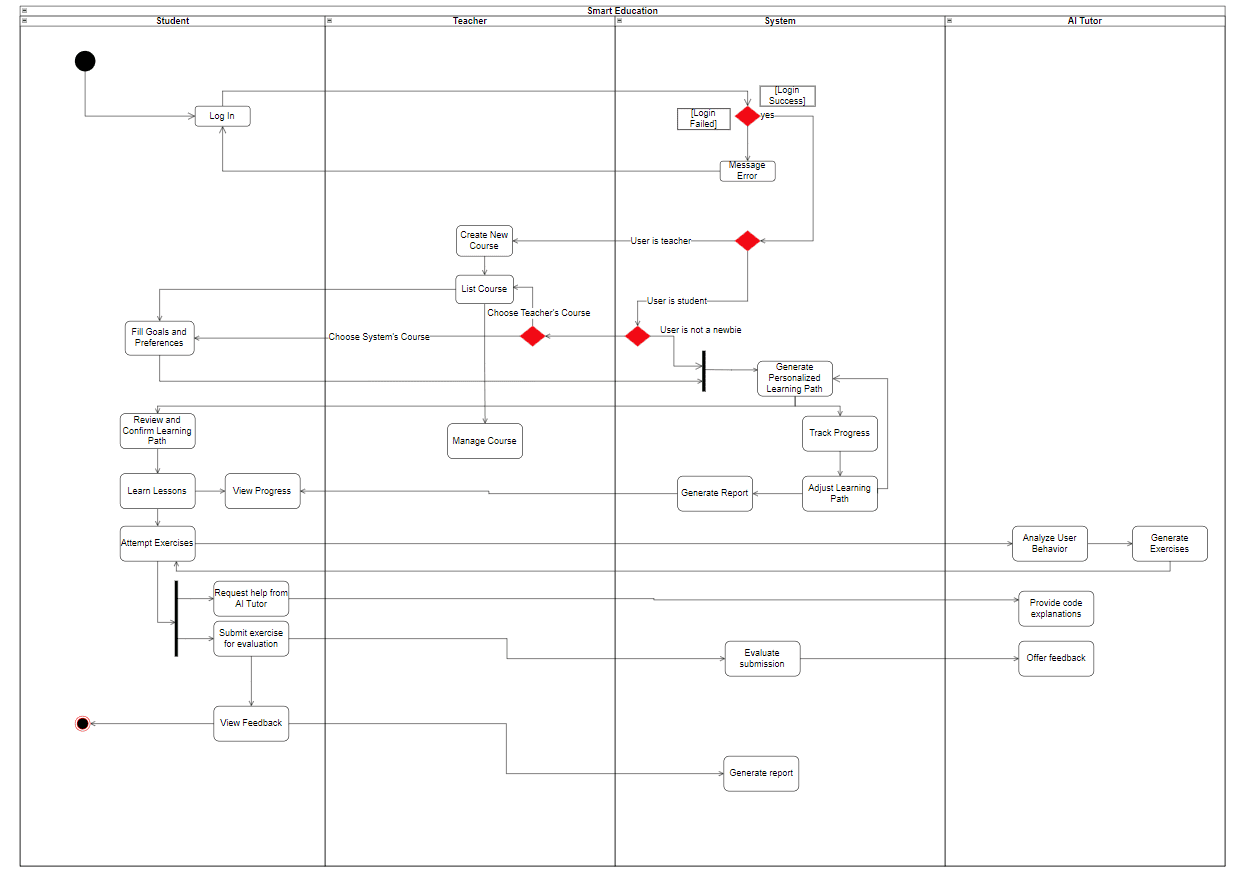
\includegraphics[width=\linewidth]{Images/Anh/activity.png}
    \caption{Activity diagram}
    \label{fig:enter-label}
\end{figure}
Activity diagram mô tả quy trình tương tác giữa bốn Actors: \textbf{\textit{Student (Học sinh), Teacher (Giáo viên), System (Hệ thống), và AI Tutor (Gia sư AI)}} trong hệ thống giáo dục thông minh. \par Học sinh bắt đầu bằng việc đăng nhập và tùy thuộc vào vai trò của họ (giáo viên hoặc học sinh), các hành động khác nhau sẽ diễn ra. Giáo viên có thể tạo khóa học mới hoặc chọn khóa học hiện có để quản lý, trong khi học sinh sẽ xác định mục tiêu học tập và xác nhận lộ trình học do hệ thống đề xuất. Sau đó, học sinh có thể học bài, thực hiện bài tập, và nếu cần có thể yêu cầu trợ giúp từ AI Tutor. Hệ thống cũng tự động theo dõi tiến độ học tập, điều chỉnh lộ trình và đánh giá bài nộp của học sinh. AI Tutor hỗ trợ bằng cách phân tích hành vi, giải thích mã code, và tạo bài tập phù hợp.
\subsection{Use case diagrams}
\begin{figure}[H]
    \centering
    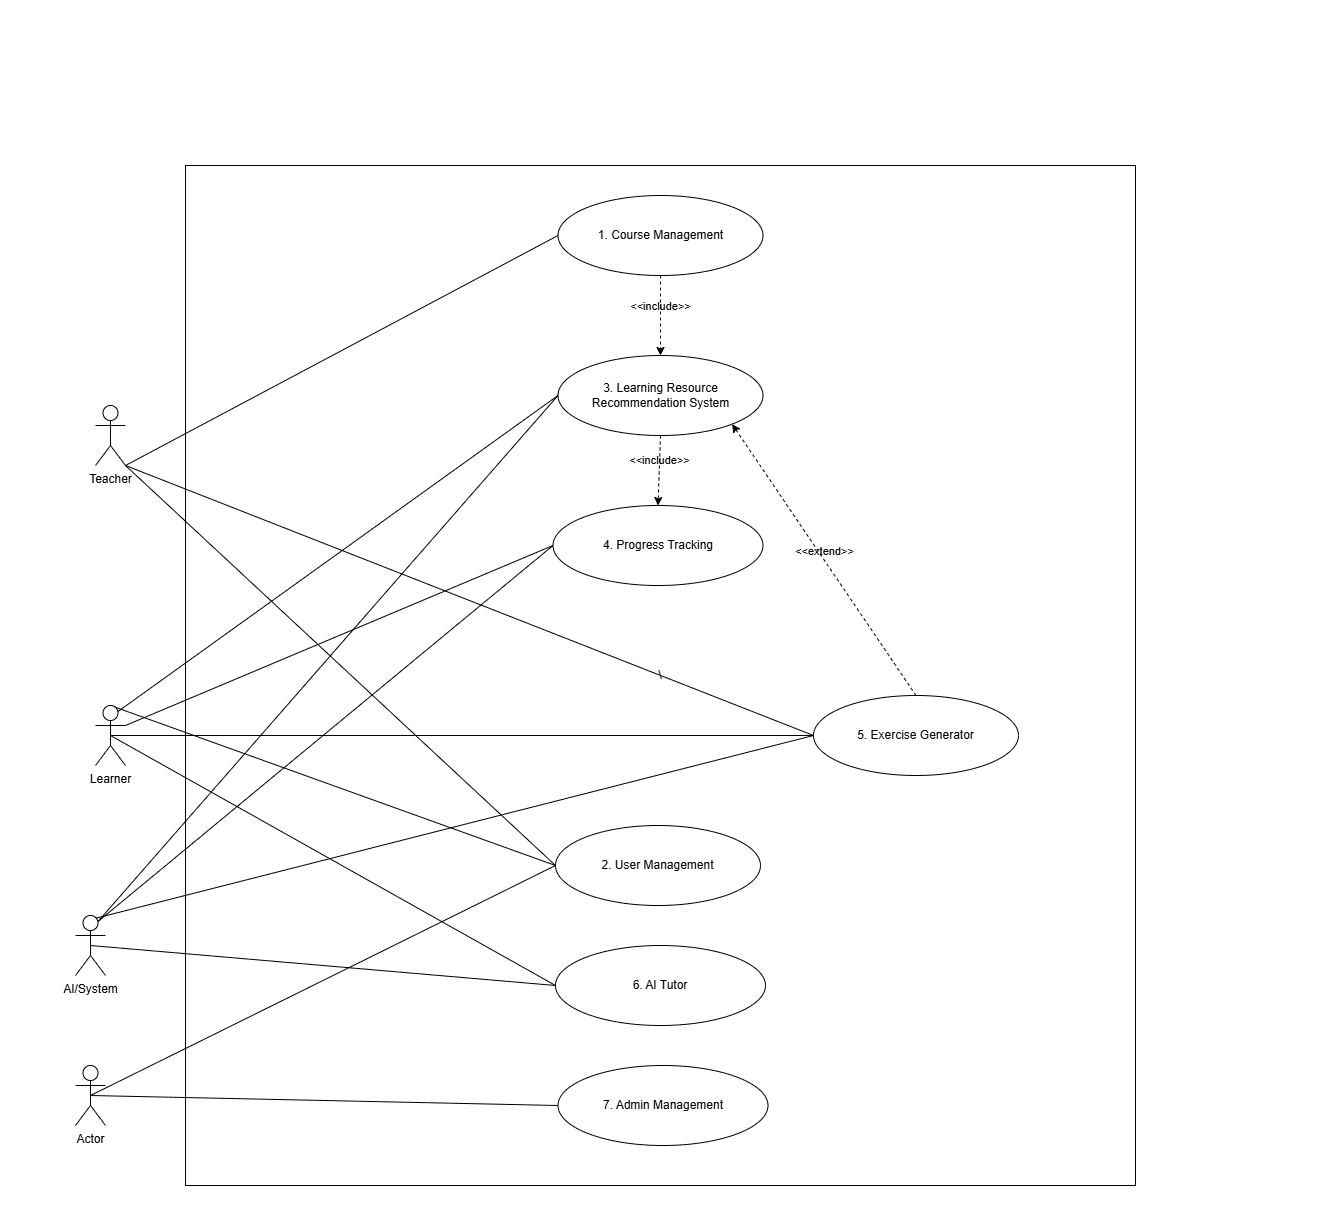
\includegraphics[scale=0.3]{Images/Usecase/usecase-All.drawio.png}
    \caption{Use case diagram}
    \label{fig:enter-label}
\end{figure}
\quad Mô hình use case tổng thể cho hệ thống học tập thông minh bao gồm ba tác nhân chính: Giáo viên, Người học, Quản trị viên và Hệ thống/AI. Các use case bao gồm Quản lý khóa học, Quản lý người dùng, Quản lý lộ trình học tập thích ứng, Theo dõi tiến độ, Tạo bài tập, Quản lý hệ thống cho Quản trị viên và Gia sư AI.
\subsubsection{Course Management}
\begin{figure}[H]
    \centering
    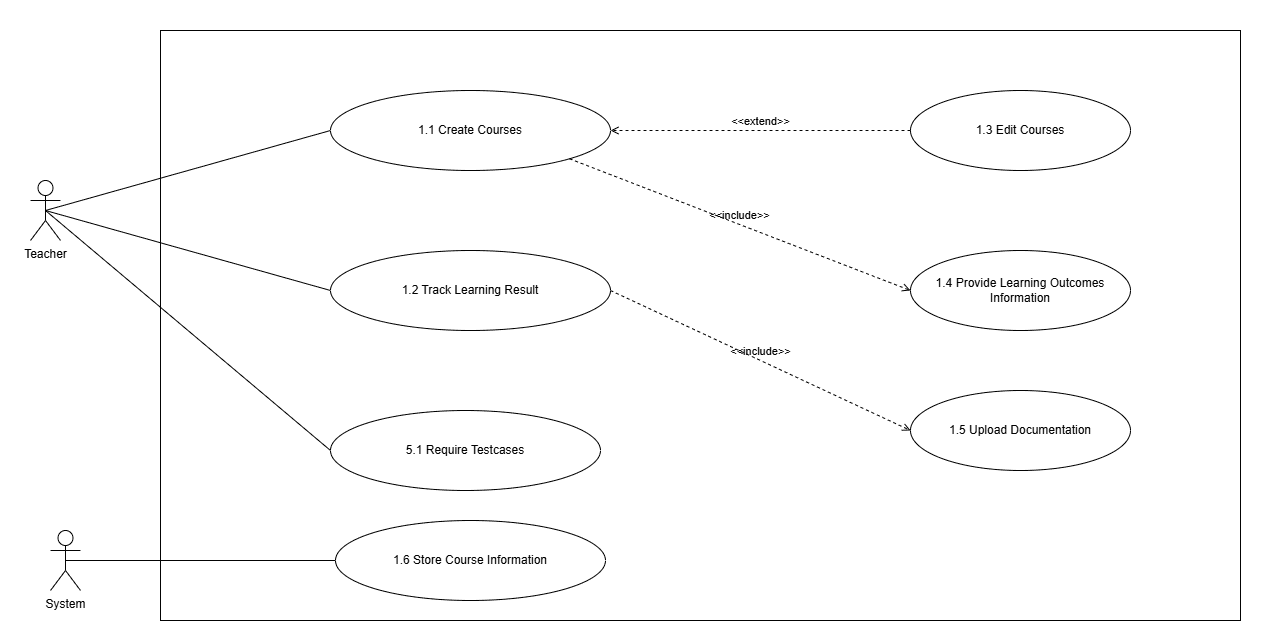
\includegraphics[scale=0.4]{Images/Usecase/usecase-Course Management.drawio.png}
    \caption{Detailed use case with id 1: Course Management}
    \label{fig:enter-label}
\end{figure}
\quad Use case \textbf{\textit{Quản lý khóa học}} bao gồm ba chức năng chính: Tạo khóa học, Theo dõi kết quả học tập và Yêu cầu bài kiểm tra. Use case  \textbf{\textit{"Chỉnh sửa khóa học"}} được mở rộng từ  \textbf{\textit{"Tạo khóa học"}}, cho thấy việc chỉnh sửa là một phần mở rộng tùy chọn của quá trình tạo khóa học. Use case diagram thể hiện các trách nhiệm chính của giáo viên trong việc quản lý khóa học trong hệ thống.
\par Ngoài ra, ở module này, Hệ thống sẽ có nhiệm vụ lưu trữ thông tin về khóa học mà giáo viên đã tạo ra. 
\subsubsection{User Management}
\begin{figure}[H]
    \centering
    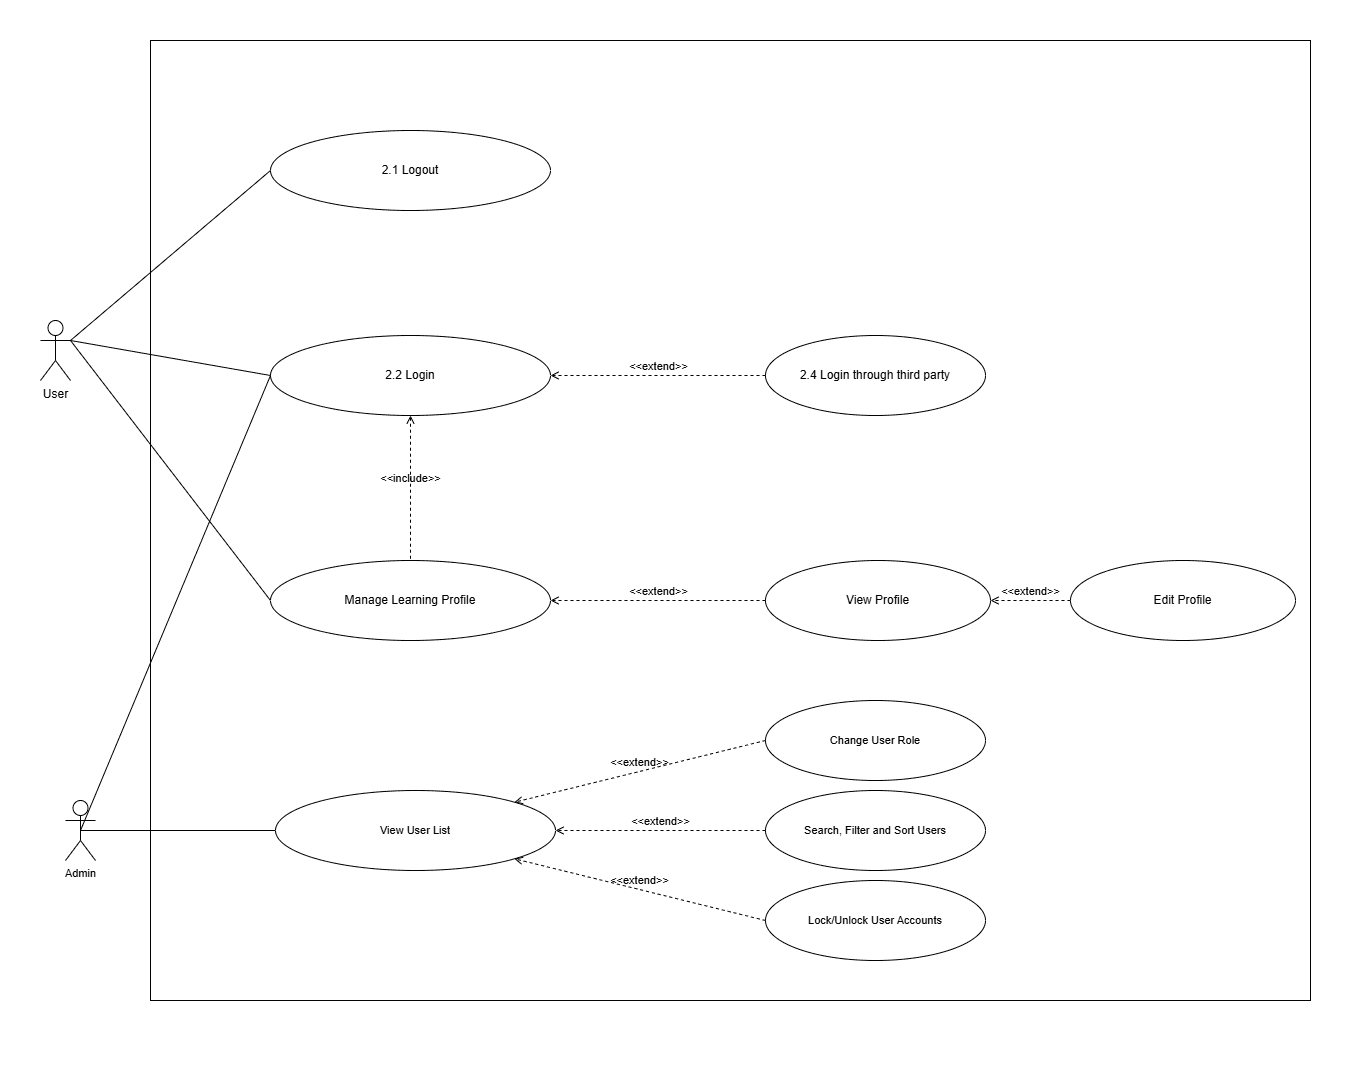
\includegraphics[scale=0.4]{Images/Usecase/usecase-User Management.drawio.png}
    \caption{Detailed use case with id 2: User Management}
    \label{fig:enter-label}
\end{figure}
\quad Use case  \textbf{\textit{Quản lý người dùng}}, tập trung vào tác nhân Người dùng bao gồm các chức năng như Đăng nhập, Đăng xuất, Quản lý hồ sơ học tập và Xem hồ sơ. Use case diagram cho thấy  \textbf{\textit{"Đăng nhập qua third-party"}} mở rộng từ use case  \textbf{\textit{"Đăng nhập"}} cơ bản, cung cấp một phương thức đăng nhập thay thế. Ngoài ra,  \textbf{\textit{"Xem hồ sơ"}} được thể hiện như một phần mở rộng của  \textbf{\textit{"Quản lý hồ sơ học tập"}}, cho thấy đây là một hành động liên quan nhưng riêng biệt. \par Quản trị viên có quyền đăng nhập bằng tài khoản của mình, từ đó \textbf{\textit{"Xem danh sách người dùng"}} sử dụng hệ thống. Ngoài ra, quản trị viên có thể \textbf{\textit{"Tìm kiếm, Lọc và Sắp xếp theo thông tin người dùng"}}, \textbf{\textit{"Vô hiệu hóa tài khoản/Kích hoạt tài khoản"}} và \textbf{\textit{" Thay đổi quyền truy cập của người dùng"}}. Ví dụ: Thay đổi từ người học sang giảng viên. 
\subsubsection{Learning Resource Recommendation System}
\begin{figure}[H]
    \centering
    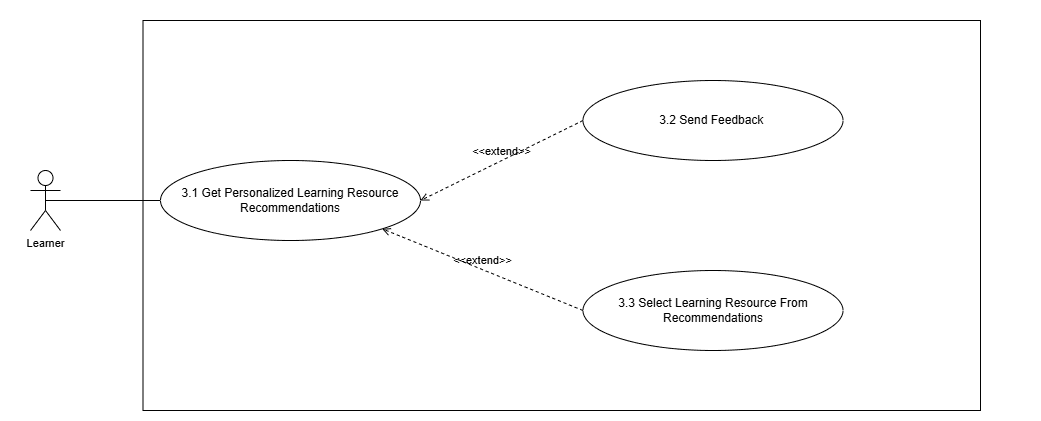
\includegraphics[scale=0.45]{Images/Usecase/usecase-Learning Resource Recommendation System - Learner.drawio.png}
    \caption{Detailed use case with id 3: Adaptive Learning Path Management of Learner Actor}
    \label{fig:enter-label}
\end{figure}
\quad Tác nhân chính trong biểu đồ trên là người học (Learner), có thể tương tác với hệ thống để nhận các đề xuất tài nguyên học tập. Use case \textbf{\textit{"Get Personalized Learning Resource Recommendations"}} cung cấp cho người học các tài nguyên học tập phù hợp với nhu cầu và lịch sử học tập của họ. Use case \textbf{\textit{"Send Feedback"}} có mối quan hệ \textbf{\textit{"<extend>"}} với \textbf{\textit{"Get Personalized Learning Resource Recommendations"}}, vì người học có thể gửi phản hồi về các tài nguyên đã được đề xuất để cải thiện hệ thống.
Use case \textbf{\textit{"Select Learning Resource From Recommendations"}} cũng mở rộng từ \textbf{\textit{"Get Personalized Learning Resource Recommendations"}}, cho phép người học tự chọn các tài nguyên mà họ thấy phù hợp với mục tiêu cá nhân.
\begin{figure}[H]
    \centering
    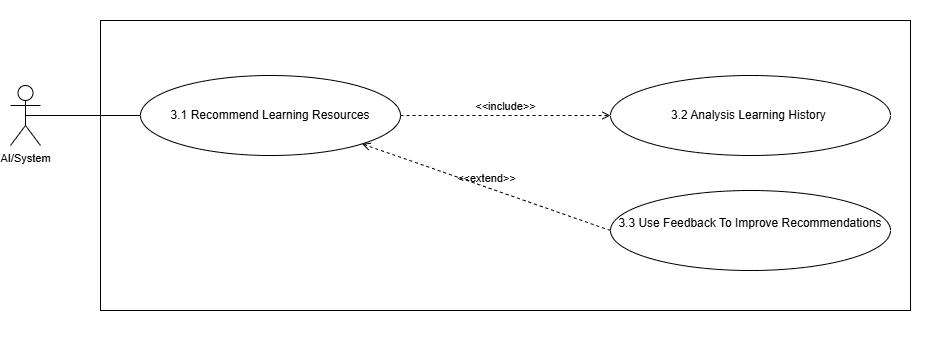
\includegraphics[scale=0.45]{Images/Usecase/usecase-Learning Resource Recommendation System - System.drawio.png}
    \caption{Detailed use case with id 3: Learning Resource Recommendation System of System Actor}
    \label{fig:enter-label}
\end{figure}
\quad Tác nhân chính là hệ thống AI, có nhiệm vụ chính là đề xuất tài nguyên học tập cá nhân hóa cho người dùng. Use case \textbf{\textit{"Recommend Learning Resources"}} bao gồm hoạt động \textbf{\textit{"Analysis Learning History"}} (phân tích lịch sử học tập), do quá trình phân tích lịch sử học tập là một phần không thể thiếu khi hệ thống tạo ra các đề xuất. Hệ thống có thể mở rộng thêm use case \textbf{\textit{"Use Feedback To Improve Recommendations"}} (sử dụng phản hồi để cải thiện đề xuất) dựa trên các phản hồi người dùng, giúp tinh chỉnh và nâng cao chất lượng đề xuất. Mối quan hệ \textbf{\textit{"<include>"}} được sử dụng giữa \textbf{\textit{"Recommend Learning Resources"}} và \textbf{\textit{"Analysis Learning History"}} vì quá trình phân tích là cần thiết. Mối quan hệ \textbf{\textit{"<extend>"}} giữa \textbf{\textit{"Recommend Learning Resources"}} và \textbf{\textit{"Use Feedback To Improve Recommendations"}} vì cải thiện đề xuất dựa trên phản hồi là một phần mở rộng có thể xảy ra tùy theo ngữ cảnh.

\subsubsection{Progress Tracking}
\begin{figure}[H]
    \centering
    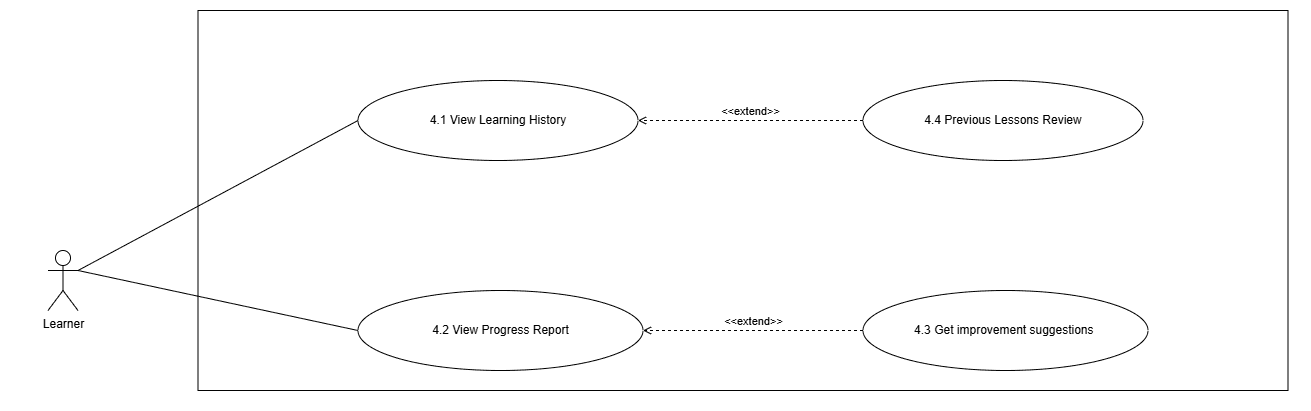
\includegraphics[scale=0.35]{Images/Usecase/usecase-Progress Tracking - Learner.drawio.png}
    \caption{Detailed use case with id 4: Progress Tracking of Learner Actor}
    \label{fig:enter-label}
\end{figure}
\quad Use case diagram trên thể hiện các chức năng  \textbf{\textit{Theo dõi tiến độ dành cho Người học}}. Có hai use case chính là  \textbf{\textit{"Xem lịch sử học tập"}} và  \textbf{\textit{"Xem báo cáo tiến độ"}}.  \textbf{\textit{"Xem lịch sử học tập"}} mở rộng đến  \textbf{\textit{"Xem lại các bài học trước đó"}}, cho phép người học ôn tập.  \textbf{\textit{"Xem báo cáo tiến độ"}} mở rộng đến  \textbf{\textit{"Nhận đề xuất cải thiện"}}, cung cấp hướng dẫn cá nhân hóa, nhấn mạnh việc theo dõi và phản hồi liên tục để hỗ trợ quá trình học tập của người dùng.
\begin{figure}[H]
    \centering
    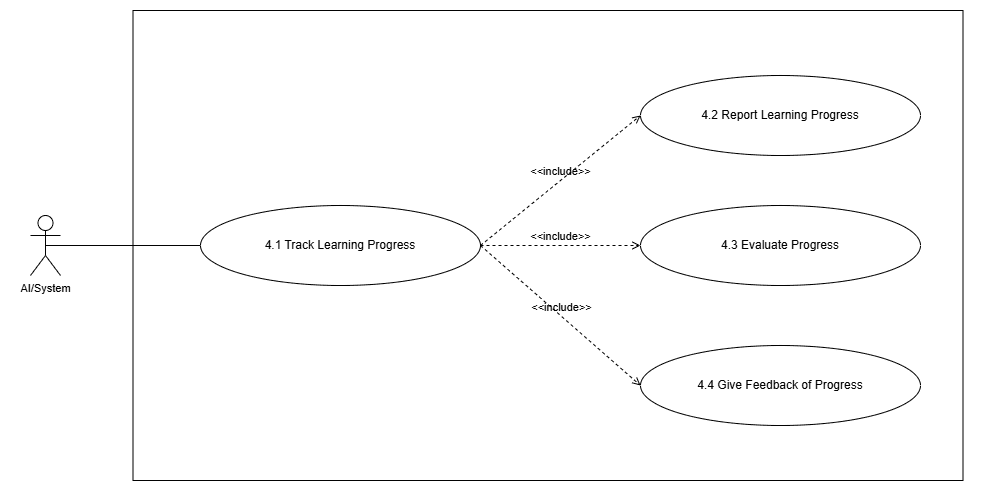
\includegraphics[scale=0.4]{Images/Usecase/usecase-Progress Tracking - System.drawio.png}
    \caption{Detailed use case with id 4: Progress Tracking of System Actor}
    \label{fig:enter-label}
\end{figure}
\quad Sơ đồ use case của hệ thống \textbf{\textit{Exercise Generator}} mô tả các tương tác giữa người dùng và hệ thống. Người học có thể yêu cầu hệ thống tạo tự động các bài tập thông qua chức năng \textbf{\textit{"Request Auto Exercise Generation"}}, và sau đó thực hiện các bài tập đó để cải thiện kỹ năng của mình thông qua \textbf{\textit{"Do Exercise"}}. Bên cạnh đó, giảng viên có thể sử dụng chức năng \textbf{\textit{"Upload Exercise"}} để tải lên các đề bài hoặc bài tập, từ đó hệ thống sẽ tự động xử lý và tạo ra các test case nhằm kiểm tra độ chính xác của bài giải thông qua \textbf{\textit{"Generate Test Cases"}}. Sau khi các test case được tạo, giảng viên có thể sử dụng chức năng \textbf{\textit{"Review Test Cases"}} để xem xét và đánh giá các test case nhằm đảm bảo chúng phù hợp với nội dung bài tập và đáp ứng được yêu cầu giảng dạy. Các chức năng này giúp hệ thống tạo ra môi trường học tập linh hoạt, hỗ trợ hiệu quả cho người học và giảng viên.
\subsubsection{Exercise Generator}
\begin{figure}[H]
    \centering
    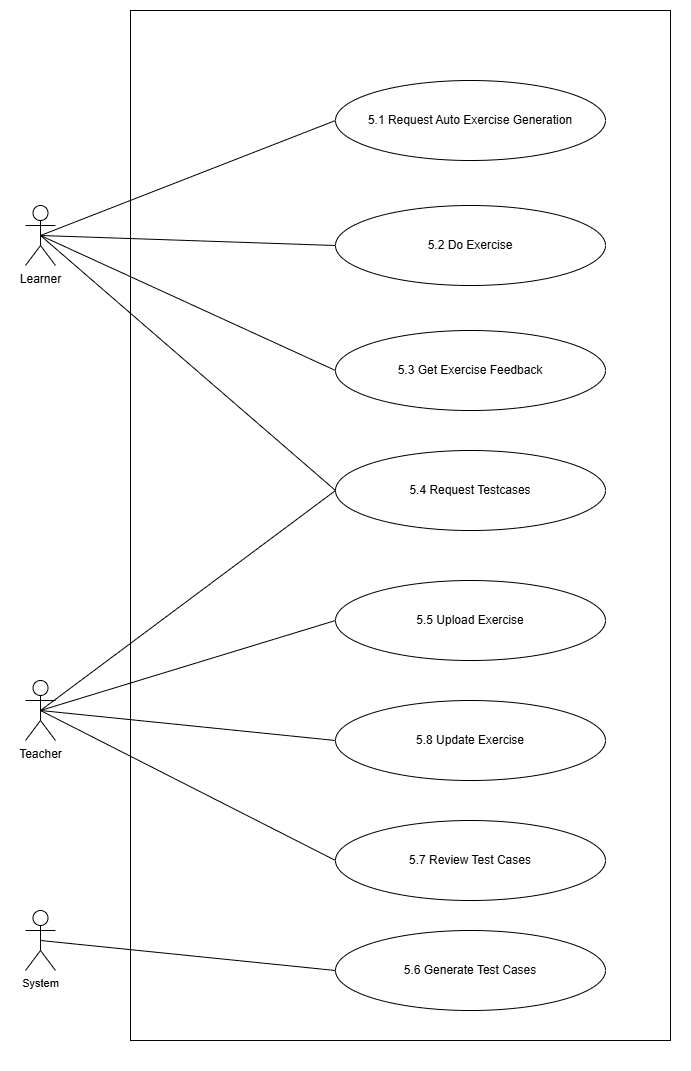
\includegraphics[scale=0.45]{Images/Usecase/usecase-Exercise Generator - Learner.drawio.png}
    \caption{Detailed use case with id 5: Exercise Generator}
    \label{fig:enter-label}
\end{figure}
\quad Use case diagram thể hiện các chức năng liên quan đến bài tập dành cho Người học. Có bốn use case chính:  \textbf{\textit{"Yêu cầu tạo bài tập tự động", "Làm bài tập", "Nhận phản hồi về bài tập", và "Yêu cầu bài kiểm tra"}}. Người học có thể yêu cầu hệ thống tạo bài tập tự động phù hợp với trình độ của họ. Sau khi làm bài tập, người học có thể nhận phản hồi để hiểu rõ hơn về kết quả của mình. Khả năng yêu cầu bài kiểm tra cho phép người học tự đánh giá kiến thức của mình khi cần.
\subsubsection{AI Tutor}
\begin{figure}[H]
    \centering
    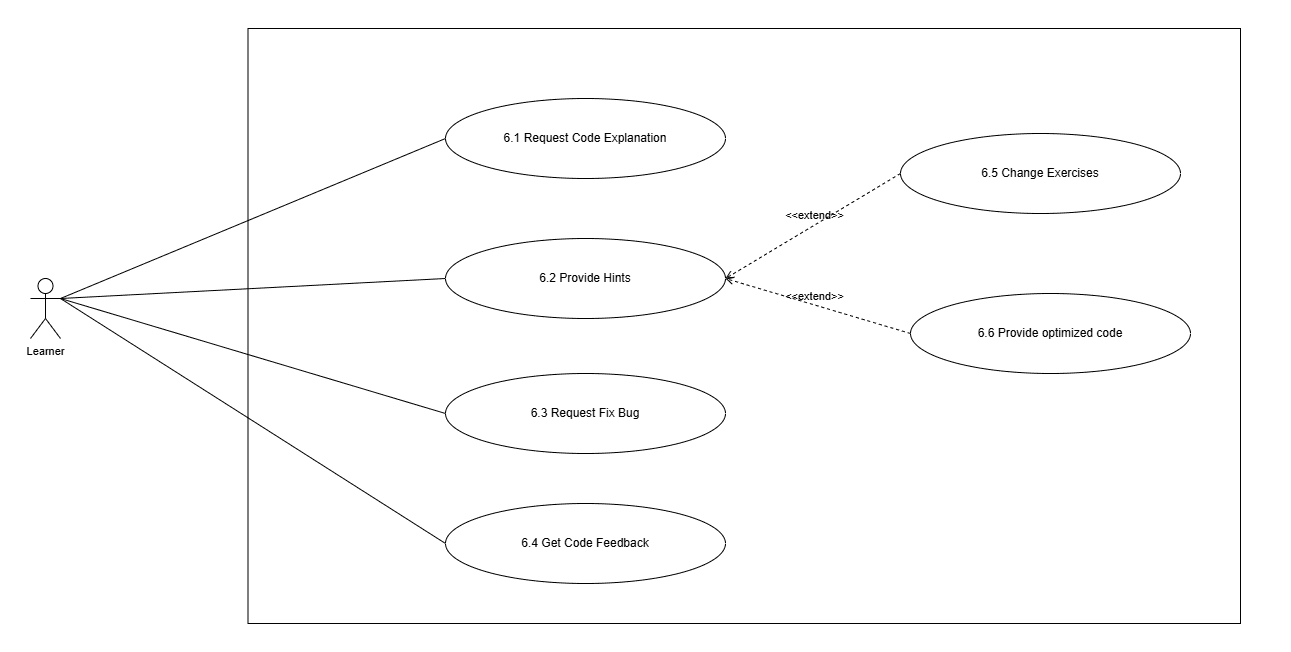
\includegraphics[scale=0.3]{Images/Usecase/usecase-AI Tutor - Learner.drawio.png}
    \caption{Detailed use case with id 6: AI Tutor of Learner Actor}
    \label{fig:enter-label}
\end{figure}
\quad Use case diagram thể hiện các chức năng của Gia sư AI dành cho Người học. Có bốn use case chính:  \textbf{\textit{"Yêu cầu giải thích mã", "Yêu cầu gợi ý", "Yêu cầu sửa lỗi", và "Nhận phản hồi về mã".}}
Người học có thể yêu cầu giải thích về mã nguồn để hiểu rõ hơn về cấu trúc và logic của code. Chức năng yêu cầu gợi ý có hai chức năng quan hệ \textbf{\textit{"extend"}} là \textbf{\textit{"Hỗ trợ chuyển đổi bài tập"}} dựa trên nhu cầu, học lực của người dùng và \textbf{\textit{"Cung cấp mã tối ưu hóa"}} giúp người học vượt qua các khó khăn trong quá trình học lập trình cũng như cải thiện tối đa kỹ thuật code của người dùng. Việc nhận phản hồi về mã giúp người học cải thiện kỹ năng lập trình của mình một cách liên tục.
\begin{figure}[H]
    \centering
    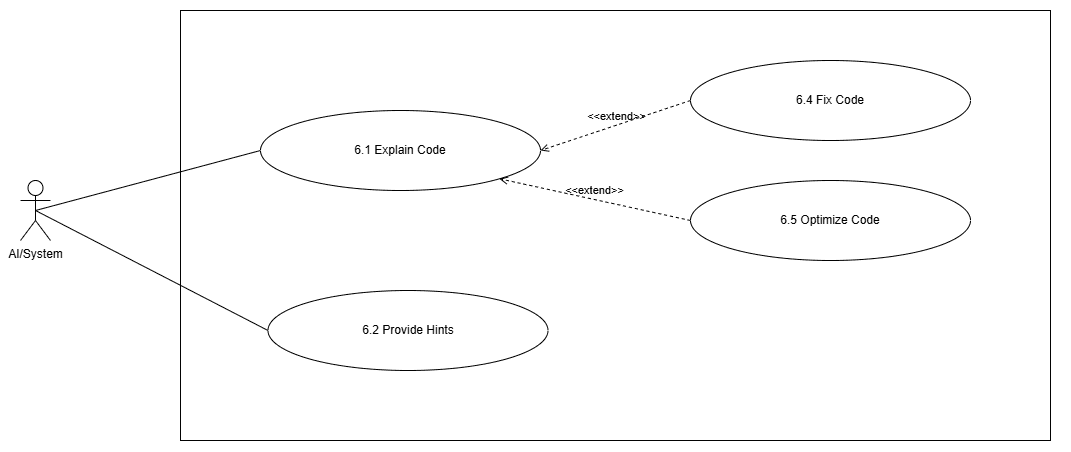
\includegraphics[scale=0.4]{Images/Usecase/usecase-AI Tutor - System.drawio.png}
    \caption{Detailed use case with id 6: AI Tutor of System Actor}
    \label{fig:enter-label}
\end{figure}
\quad Use case diagram trên mô tả  \textbf{\textit{hệ thống AI Tutor}} với vai trò hỗ trợ người dùng trong việc xử lý và hiểu mã lập trình. Hệ thống có khả năng  \textbf{\textit{giải thích mã lệnh (Use case 6.1)}} và  \textbf{\textit{cung cấp gợi ý khi người dùng gặp khó khăn (Use case 6.2)}}. Từ chức năng giải thích mã, hệ thống có thể mở rộng thêm các chức năng khác như  \textbf{\textit{sửa lỗi (Use case 6.4)}} và  \textbf{\textit{tối ưu mã lệnh (Use case 6.5)}}. Hệ thống nhằm mục tiêu hỗ trợ người dùng học lập trình hiệu quả hơn thông qua các công cụ hỗ trợ trực tiếp từ AI.
\newpage
\section{Thiết kế}
\subsection{Kiến trúc hệ thống}
\subsubsection{Phân tích kiến trúc hệ thống phổ biến hiện nay}
Hiện nay, có nhiều kiến trúc phần mềm khác nhau, mỗi loại có ưu và nhược điểm riêng, phù hợp với các loại dự án và yêu cầu cụ thể. Dưới đây là một số kiến trúc phần mềm phổ biến và các điểm chính của chúng:
\begin{enumerate}
    \item Kiến trúc Monolithic
    \begin{itemize}
        \item \textbf{\textit{Định nghĩa:}} Kiến trúc monolithic là một mô hình truyền thống trong đó toàn bộ ứng dụng được xây dựng như một đơn vị duy nhất, tích hợp chặt chẽ.
        \item \textbf{\textit{Điểm chính:}} 
        \begin{itemize}
            \item Đơn giản để phát triển, triển khai và kiểm thử
            \item Hiệu suất tốt do không có overhead của network calls
            \item Khó mở rộng và bảo trì khi ứng dụng phức tạp
            \item Khó áp dụng công nghệ mới cho từng phần của ứng dụng
        \end{itemize}
        \item \textbf{\textit{Ví dụ:}} Một ứng dụng web PHP truyền thống, nơi tất cả chức năng (UI, business logic, data access) đều nằm trong cùng một codebase.
    \end{itemize}
    \item Kiến trúc Microservices
    \begin{itemize}
        \item \textbf{\textit{Định nghĩa:}} Kiến trúc microservices chia nhỏ ứng dụng thành các dịch vụ độc lập, mỗi dịch vụ chịu trách nhiệm cho một chức năng cụ thể và có thể được phát triển, triển khai độc lập.
        \item \textbf{\textit{Điểm chính:}} 
        \begin{itemize}
            \item Dễ dàng mở rộng và bảo trì từng service riêng biệt
            \item Cho phép sử dụng công nghệ phù hợp nhất cho mỗi service
            \item Tăng cường khả năng chịu lỗi của hệ thống
            \item Phức tạp hơn trong việc quản lý và điều phối các service
        \end{itemize}
        \item \textbf{\textit{Ví dụ:}} Netflix sử dụng kiến trúc microservices, với các service riêng biệt cho việc xử lý video, quản lý người dùng, đề xuất nội dung, v.v.
    \end{itemize}
    \item Kiến trúc Client-Server
    \begin{itemize}
        \item \textbf{\textit{Định nghĩa:}} Kiến trúc client-server chia ứng dụng thành hai phần chính: client (trình bày và tương tác người dùng) và server (xử lý logic nghiệp vụ và lưu trữ dữ liệu).
        \item \textbf{\textit{Điểm chính:}} 
        \begin{itemize}
            \item Phân tách rõ ràng giữa client và server
            \item Dễ dàng mở rộng server để đáp ứng nhu cầu người dùng
            \item Cải thiện bảo mật thông qua kiểm soát truy cập tại server
            \item Phụ thuộc vào kết nối mạng giữa client và server
        \end{itemize}
        \item \textbf{\textit{Ví dụ:}} Một ứng dụng web với frontend (React) và backend (Node.js) giao tiếp qua RESTful API.
    \end{itemize}
    \item Kiến trúc Event-Driven
    \begin{itemize}
        \item \textbf{\textit{Định nghĩa:}} Kiến trúc event-driven là một mô hình trong đó việc tạo ra, phát hiện, tiêu thụ và phản ứng với các sự kiện là cốt lõi của hệ thống.
        \item \textbf{\textit{Điểm chính:}} 
        \begin{itemize}
            \item Tách rời các thành phần hệ thống, giảm sự phụ thuộc trực tiếp
            \item Khả năng mở rộng và linh hoạt cao
            \item Dễ dàng thêm chức năng mới mà không ảnh hưởng đến các thành phần hiện có
            \item Có thể phức tạp trong việc theo dõi luồng xử lý và debug
        \end{itemize}
        \item \textbf{\textit{Ví dụ:}} Hệ thống thương mại điện tử, khi một đơn hàng được đặt, một sự kiện "OrderPlaced" được phát ra, kích hoạt các quy trình xử lý khác như cập nhật kho, gửi email xác nhận, v.v.
    \end{itemize}
    \item Kiến trúc Serverless
    \begin{itemize}
        \item \textbf{\textit{Định nghĩa:}} Kiến trúc serverless cho phép phát triển và chạy ứng dụng mà không cần quản lý trực tiếp máy chủ, tập trung vào việc viết code cho các chức năng (functions) cụ thể.
        \item \textbf{\textit{Điểm chính:}} 
        \begin{itemize}
            \item Giảm chi phí vận hành và bảo trì hạ tầng
            \item Tự động mở rộng theo nhu cầu sử dụng
            \item Chỉ trả tiền cho tài nguyên thực sự sử dụng
            \item Có thể gặp vấn đề về cold start và vendor lock-in
        \end{itemize}
        \item \textbf{\textit{Ví dụ:}} Một ứng dụng xử lý ảnh sử dụng AWS Lambda để thực hiện các tác vụ như resize, filter, và lưu trữ ảnh khi người dùng tải lên.
    \end{itemize}
\end{enumerate}

\subsubsection{Lựa chọn kiến trúc hệ thống}
Dựa trên yêu cầu của hệ thống, nhóm quyết định sử dụng kiến trúc Client-Server. Cụ thể như sau:
\begin{enumerate}
    \item Client Tier:
    \begin{itemize}
        \item \textbf{Frontend:} Ứng dụng Vue.js cung cấp giao diện người dùng cho sinh viên, giảng viên và admin.
        \item \textbf{Chức năng:} Hiển thị nội dung học tập, quản lý khóa học, bài tập, lộ trình học tập và tương tác với người dùng.
        \item \textbf{Tương tác:} Giao tiếp với server thông qua RESTful API.
    \end{itemize}
    \item Server Tier:
    \begin{enumerate}
        \item \textbf{API Layer:}
        \begin{itemize}
            \item \textbf{Framework:} FastAPI xử lý các yêu cầu từ client.
            \item \textbf{Chức năng:}
            \begin{itemize}
                \item \textit{User Management:} Quản lý thông tin người dùng, xác thực và phân quyền.
                \item \textit{Course Management:} CRUD cho khóa học, module, bài học và nội dung học tập.
                \item \textit{Recommendation System:} Đề xuất tài nguyên học tập dựa trên dữ liệu người dùng.
                \item \textit{AI Tutor:} Tích hợp LangChain để hỗ trợ giải đáp thắc mắc và giải thích mã nguồn.
                \item \textit{Exercise Generation:} Tạo bài tập và test cases tự động bằng LangChain.
                \item \textit{Progress Tracking:} Theo dõi tiến độ học tập và tạo báo cáo.
            \end{itemize}
        \end{itemize}
        \item \textbf{Persistence Layer:}
        \begin{itemize}
            \item \textbf{PostgreSQL:} Lưu trữ dữ liệu có cấu trúc như thông tin người dùng, khóa học, bài học và tiến độ học tập.
            \item \textbf{AWS S3:} Lưu trữ tài liệu học tập, video bài giảng và các tài nguyên khác.
        \end{itemize}
        \item \textbf{Caching Layer:}
        \begin{itemize}
            \item \textbf{Redis:} Lưu trữ tạm thời dữ liệu thường xuyên truy cập để cải thiện hiệu suất và giảm tải cho cơ sở dữ liệu.
        \end{itemize}
    \end{enumerate}
\end{enumerate}

\textbf{\textit{Phân tích nguyên nhân:}}
\begin{itemize}
    \item \textbf{Phân tách rõ ràng:} Kiến trúc Client-Server tách biệt giữa giao diện người dùng (client) và logic nghiệp vụ/dữ liệu (server), giúp dễ dàng phát triển và bảo trì.
    \item \textbf{Dễ mở rộng:} Server có thể được mở rộng bằng cách tăng tài nguyên hoặc thêm các instance FastAPI khi số lượng người dùng tăng.
    \item \textbf{Bảo mật:} Server kiểm soát truy cập và xác thực, đảm bảo an toàn dữ liệu.
    \item \textbf{Hiệu quả:} Sử dụng Redis để tối ưu hiệu suất truy vấn và AWS S3 để quản lý tài nguyên lớn như video, tài liệu.
\end{itemize}

\textbf{\textit{Không dùng:}}
\begin{itemize}
    \item \textit{Monolithic:} Khó mở rộng, bảo trì và tích hợp công nghệ mới khi hệ thống phát triển.
    \item \textit{Microservices:} Phức tạp trong quản lý nhiều dịch vụ, không cần thiết cho quy mô hiện tại của hệ thống.
    \item \textit{Event-Driven:} Phức tạp trong việc đồng bộ và theo dõi trạng thái, không phù hợp với yêu cầu tương tác trực tiếp.
    \item \textit{Serverless:} Phụ thuộc nhà cung cấp, chi phí cao khi tải tăng và hạn chế tùy chỉnh hiệu suất.
\end{itemize}

\textbf{\textit{Luồng hoạt động:}}
\begin{itemize}
    \item Người dùng tương tác với giao diện Vue.js (Client Tier).
    \item Client gửi các request đến server thông qua RESTful API.
    \item FastAPI (Server Tier) xử lý logic nghiệp vụ, truy vấn PostgreSQL hoặc AWS S3 để lấy/lưu dữ liệu.
    \item Redis được sử dụng để cache dữ liệu, giảm thời gian phản hồi.
    \item Kết quả được trả về client để hiển thị cho người dùng.
\end{itemize}

\textbf{\textit{Tóm lại,}} kiến trúc Client-Server được chọn vì sự đơn giản, khả năng mở rộng và tính bảo mật cao, phù hợp với yêu cầu của hệ thống học tập trực tuyến thông minh. Việc sử dụng Vue.js, FastAPI, PostgreSQL, AWS S3 và Redis đảm bảo hiệu suất, linh hoạt và dễ dàng bảo trì trong tương lai.
\begin{figure}[H]
    \centering
    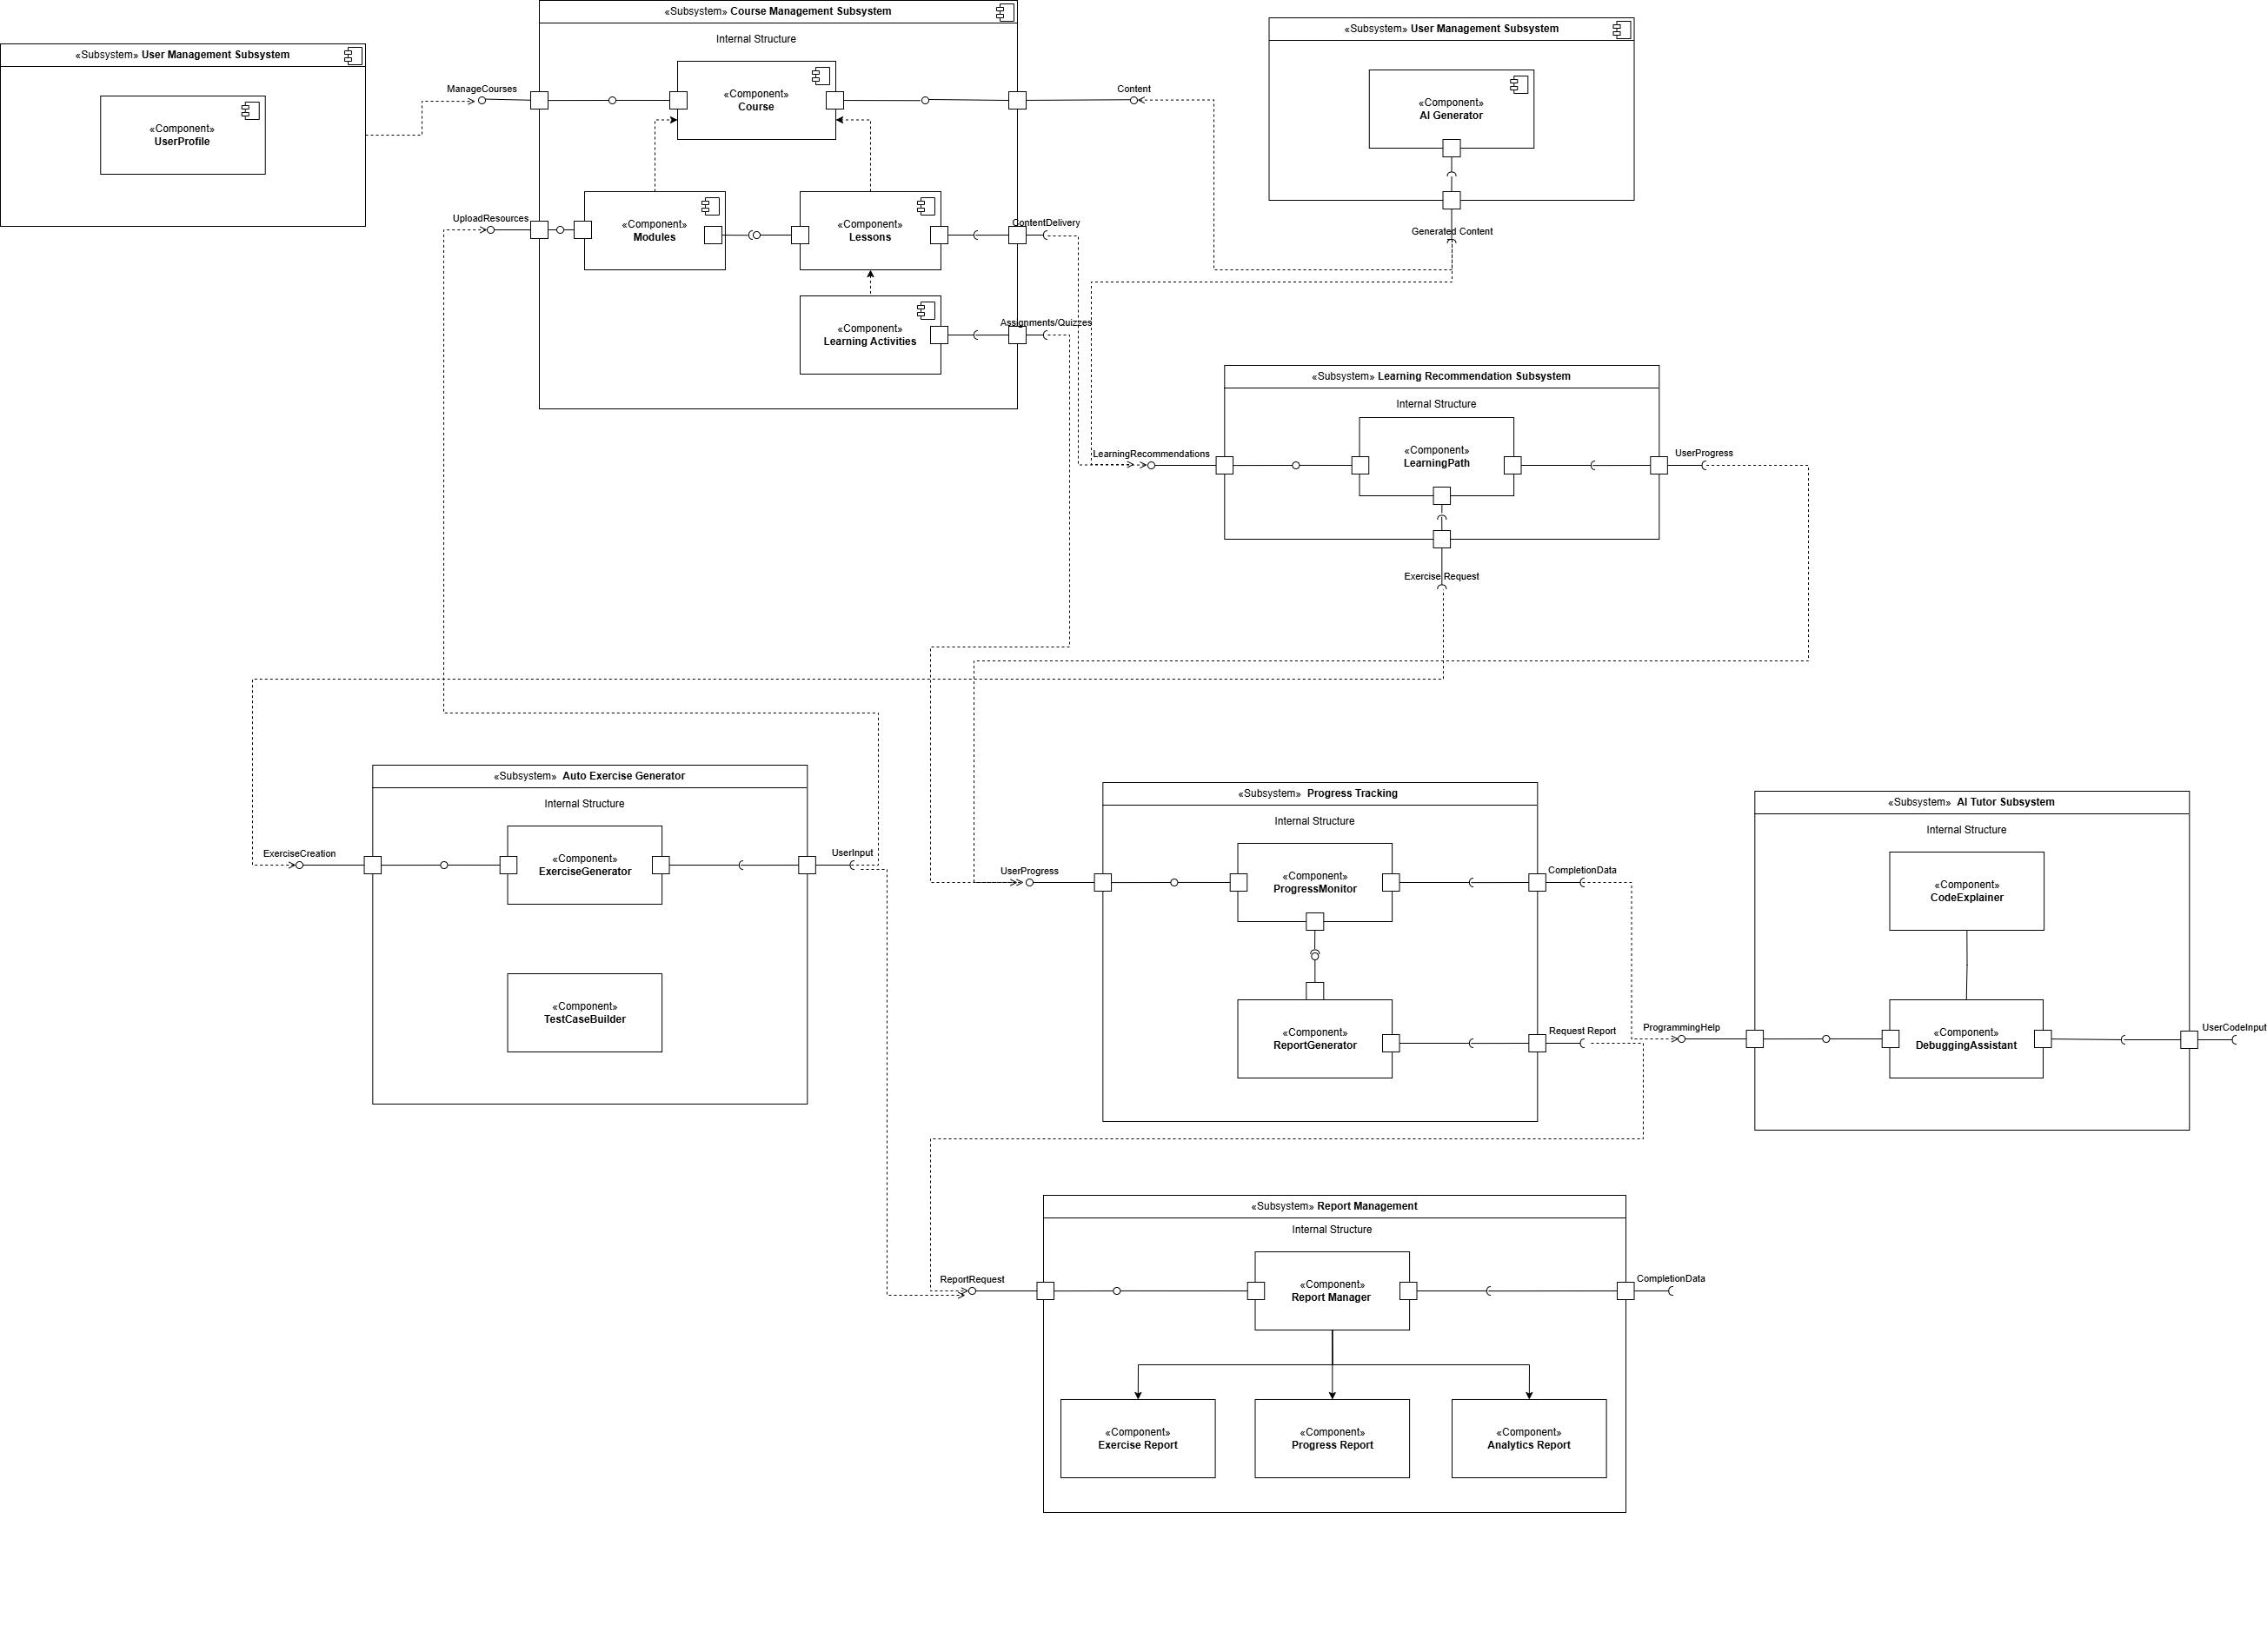
\includegraphics[width=\linewidth]{Images/component_diagram/component-All.drawio.png}
    \caption{Component-based Diagram cho toàn bộ hệ thống}
    \label{fig:enter-label}
\end{figure}
\begin{figure}[H]
    \centering
    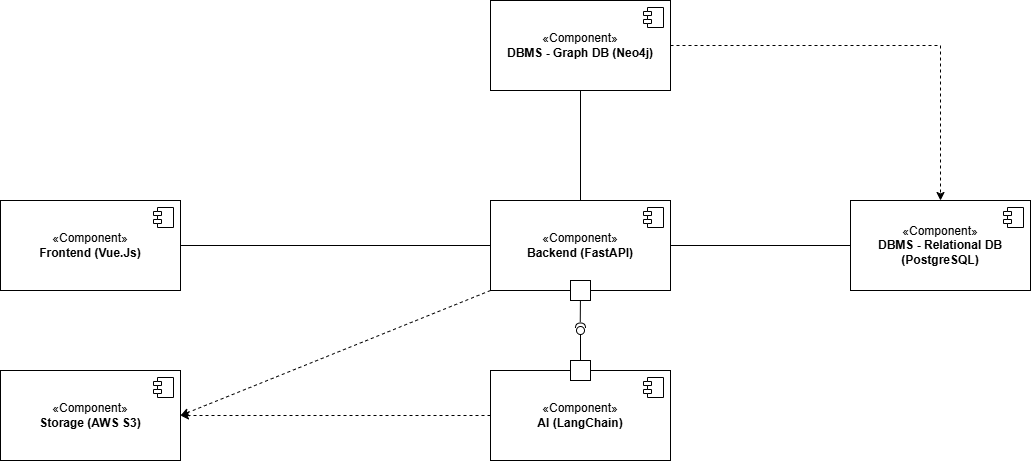
\includegraphics[width=\linewidth]{Images/component_diagram/component-Selected technologies.drawio.png}
    \caption{Component-based Diagram cho những công nghệ được chọn}
    \label{fig:enter-label}
\end{figure}
\newpage
\section{Database}
\subsection{EER diagram}
\begin{figure}[h!]
    \centering
    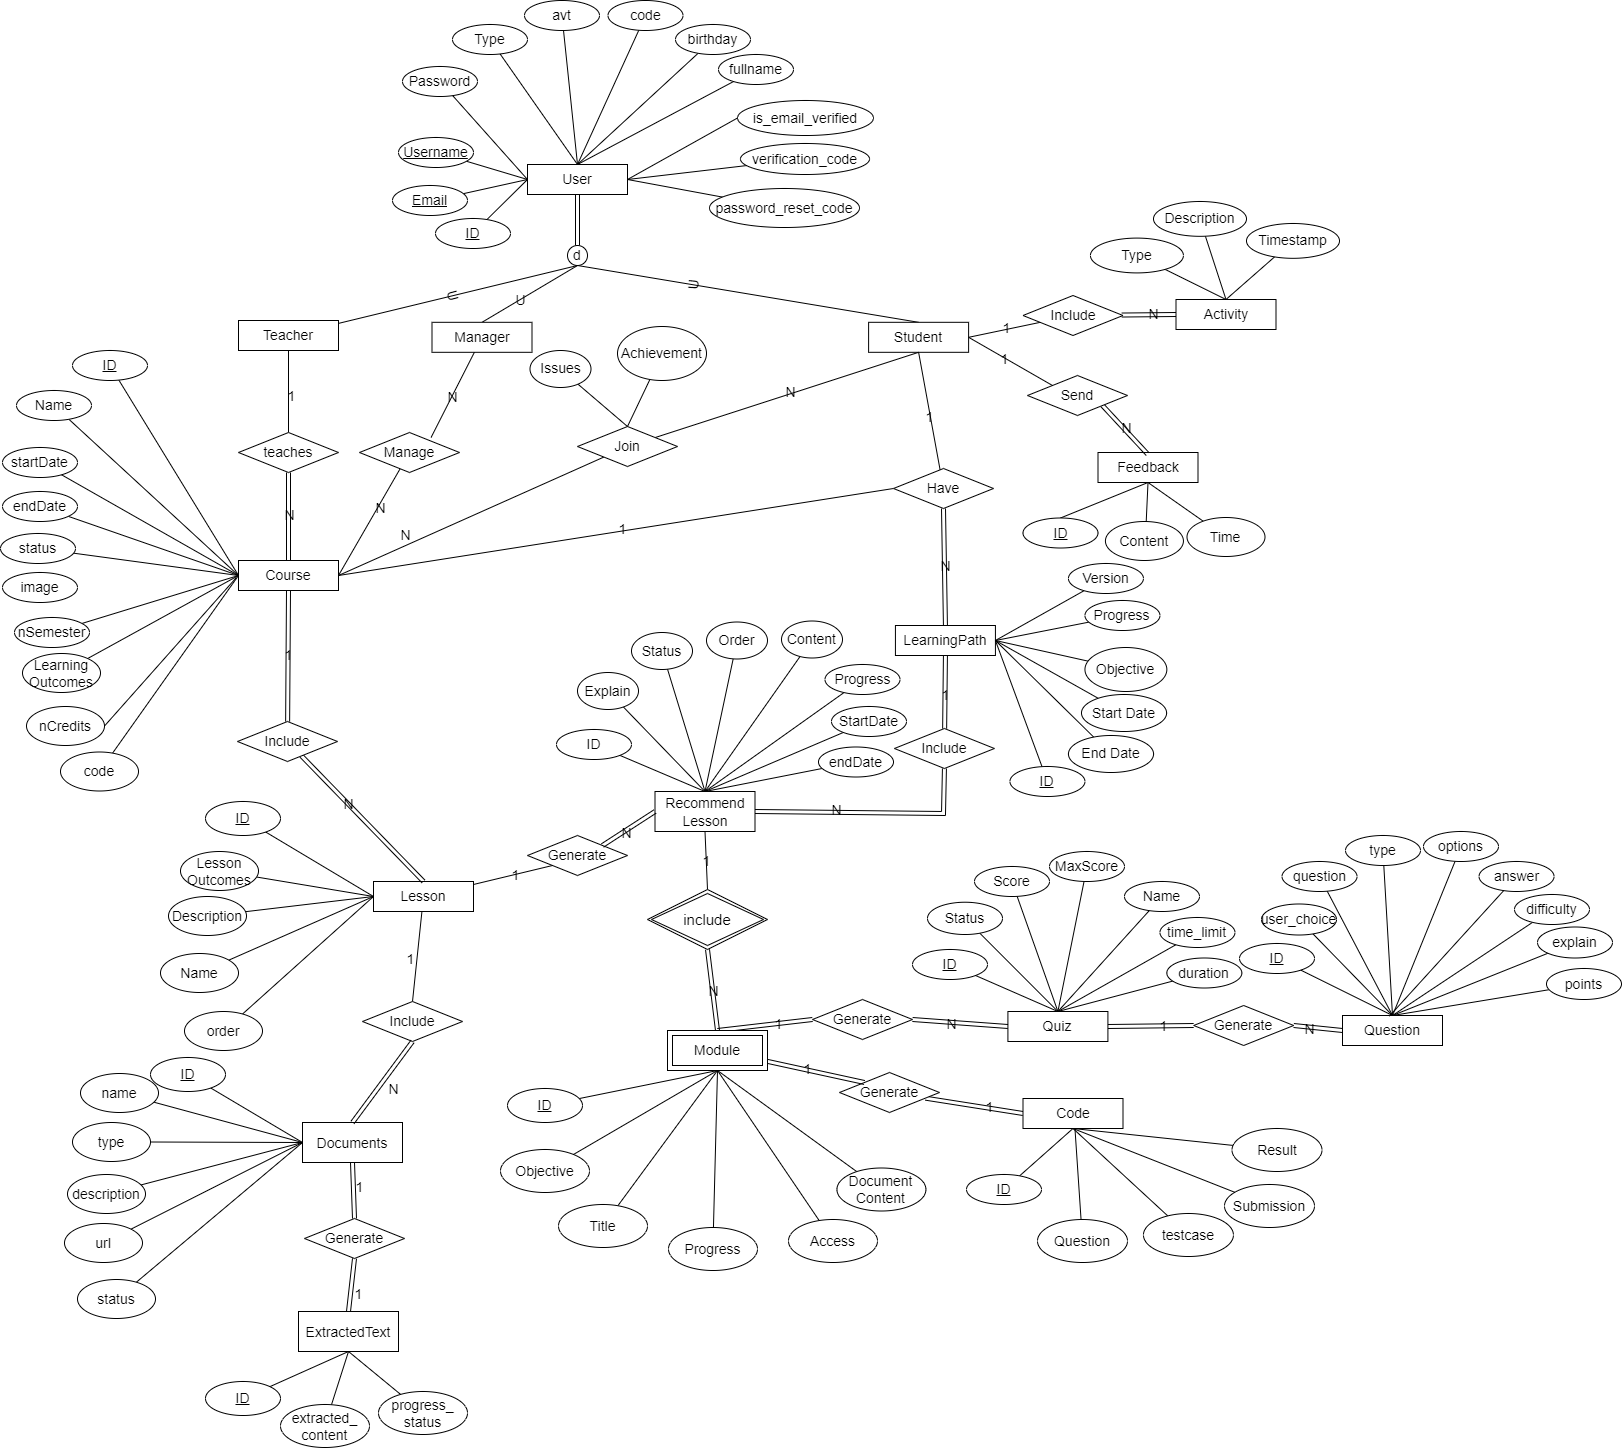
\includegraphics[width=\linewidth]{Images/Anh/EER.png}
    \caption{Sơ đồ EER của hệ thống}
    \label{fig:enter-label}
\end{figure}
\begin{enumerate}

    \item User có ba loại con: Teacher, Manager, và Student. Mỗi loại người dùng có các mối quan hệ khác nhau với các thực thể khác trong hệ thống:
    \begin{itemize}
        \item Student có các mối quan hệ sau:
        \begin{itemize}
            \item Include một hoặc nhiều Activity.
            \item Send nhiều Feedback cho hệ thống.
            \item Submit nhiều Exercise để thực hành.
            \item Join nhiều Course để tham gia các khóa học.
            \item Bookmark nhiều Lesson để lưu trữ các bài học quan trọng.
        \end{itemize}
        \item Teacher có thể Upload nhiều Course vào hệ thống để giảng dạy.
        \item Manager có thể Manage nhiều Course trong hệ thống, tức là có quyền quản lý các khóa học.
    \end{itemize}
    \item Course bao gồm nhiều Lesson, và mỗi khóa học có thể Include nhiều bài học khác nhau. Mỗi học viên (Student) có thể tham gia một khóa học và cho mỗi khóa học, họ sẽ có một LearningPath riêng biệt. Mối quan hệ này thể hiện rằng mỗi học viên có một lộ trình học tập cho mỗi khóa học mà họ tham gia.
    \item Lesson có thể Specialize thành Recommend Lesson, tức là các bài học có thể bao gồm các đề xuất học tập cho học viên. Mỗi bài học cũng có thể Include nhiều Module.
    \item LearningPath của mỗi học viên sẽ Have nhiều Recommend Lesson. Các lộ trình học tập này sẽ dẫn dắt học viên thông qua các bài học được đề xuất trong suốt quá trình học.
    \item Recommend Lesson có thể Include nhiều Module, tức là mỗi bài học được đề xuất có thể bao gồm nhiều mô-đun khác nhau để hỗ trợ học viên học tập một cách chi tiết hơn.
    \item Module có thể Generate nhiều Quiz để đánh giá kết quả học tập của học viên. Mỗi mô-đun cũng có thể Generate một tài liệu (Document) duy nhất liên quan đến nội dung học.
    \item Quiz chứa các câu hỏi và bài kiểm tra học viên, có thể bao gồm các phản hồi từ LLM Response, cung cấp thông tin về tên, độ khó, câu hỏi, câu trả lời, các lựa chọn, và hình ảnh liên quan đến bài kiểm tra.
    \item Document có thể được tạo ra từ các mô-đun và cũng có phản hồi từ LLM Response, giúp cung cấp thêm tài liệu học tập cho học viên.
    \item Activity bao gồm các hành động của người dùng trong hệ thống, và mỗi hoạt động có thể được Include bởi một hoặc nhiều User, đặc biệt là học viên.
    \item Feedback là thông tin phản hồi từ học viên gửi đến hệ thống và có thể được Send từ nhiều User, đặc biệt là từ học viên để cải thiện chất lượng giảng dạy và học tập.
\end{enumerate}
\newpage
\subsection{Lược đồ CSDL quan hệ ánh xạ}
\begin{figure}[h!]
    \centering
    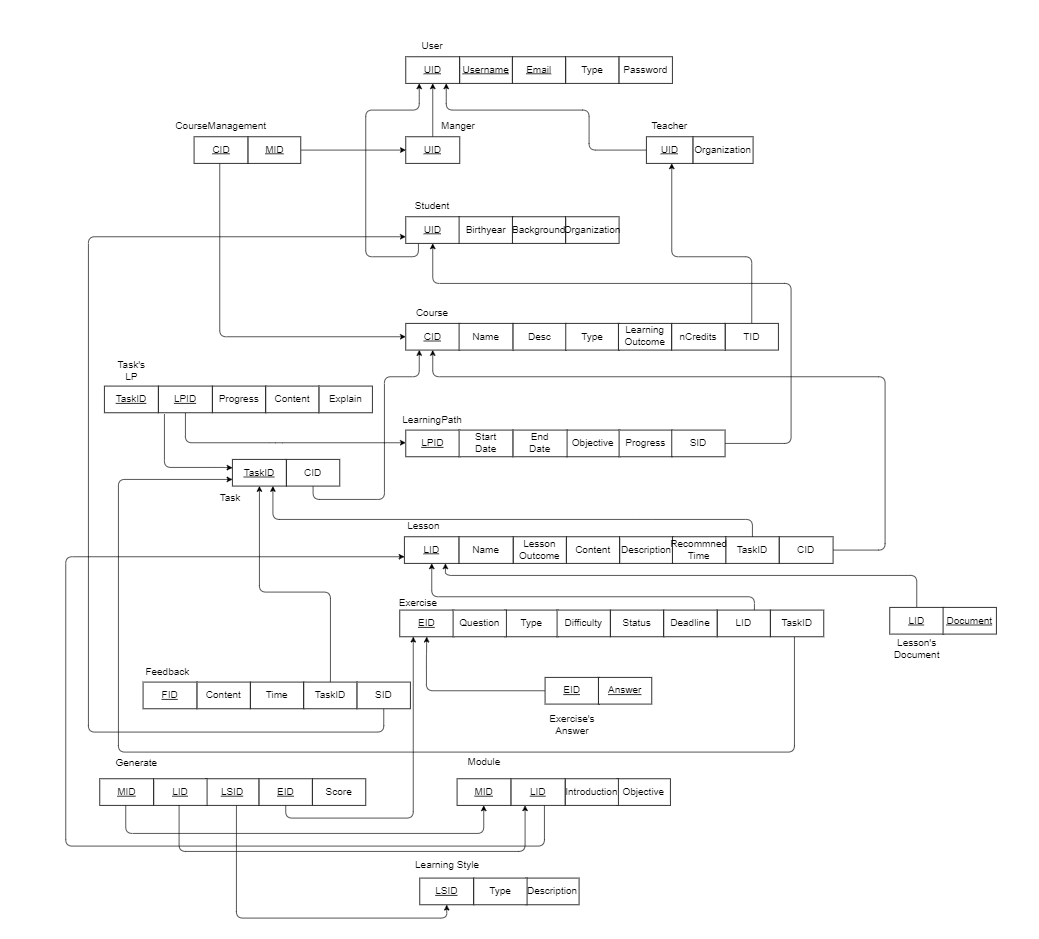
\includegraphics[width=\linewidth]{Images/Anh/mapping.png}
    \caption{Lược đồ CSDL quan hệ ánh xạ của hệ thống}
    \label{fig:enter-label}
\end{figure}
\newpage
\subsection{Class diagram}
\begin{figure}[h!]
    \centering
    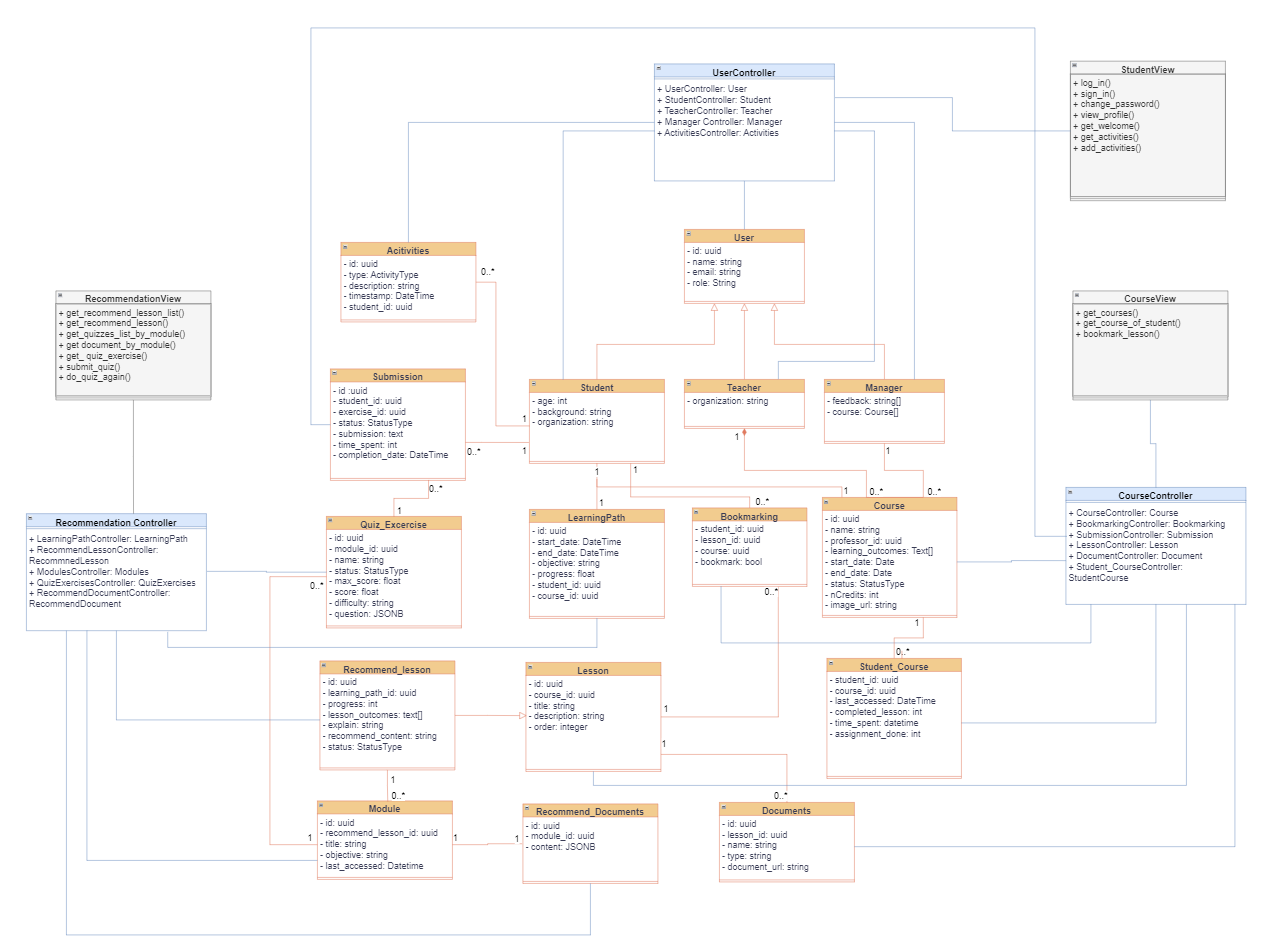
\includegraphics[width=\linewidth]{Images/Anh/classdiagram.png}
    \caption{Class diagram hiện thực của hệ thống}
    \label{fig:enter-label}
\end{figure}
Class diagram được thiết kế theo mô hình MVC mô tả một hệ thống học tập thông minh với ba vai trò chính là sinh viên, giáo viên và quản trị viên, tất cả đều kế thừa từ lớp người dùng (User). Mỗi người dùng có các chức năng cơ bản như đăng nhập, đăng xuất và cập nhật hồ sơ. Sinh viên chọn theo học khóa học của giảng viên, thực hiện bài tập, và theo dõi tiến độ học tập của mình. Lộ trình học tập bao gồm bài tập được cá nhân hóa cho từng sinh viên. Giáo viên chịu trách nhiệm tạo và quản lý các khóa học, bao gồm việc thêm bài tập, theo dõi kết quả học tập của sinh viên, và tạo ra các bộ câu hỏi kiểm tra. Quản trị viên có quyền quản lý toàn bộ hệ thống, bao gồm khóa học và người dùng, cũng như giải quyết các thắc mắc từ người dùng.
AI được sử dụng để hỗ trợ quá trình học tập thông qua việc tự động tạo lộ trình học tập và bài tập. AI dựa vào dữ liệu từ các tài liệu học tập, câu hỏi và đáp án có sẵn, cũng như các bài tập lập trình để cá nhân hóa trải nghiệm học cho người dùng.
\subsection{Sitemap}
\subsubsection{Sinh viên}
\begin{figure}[H]
    \centering
    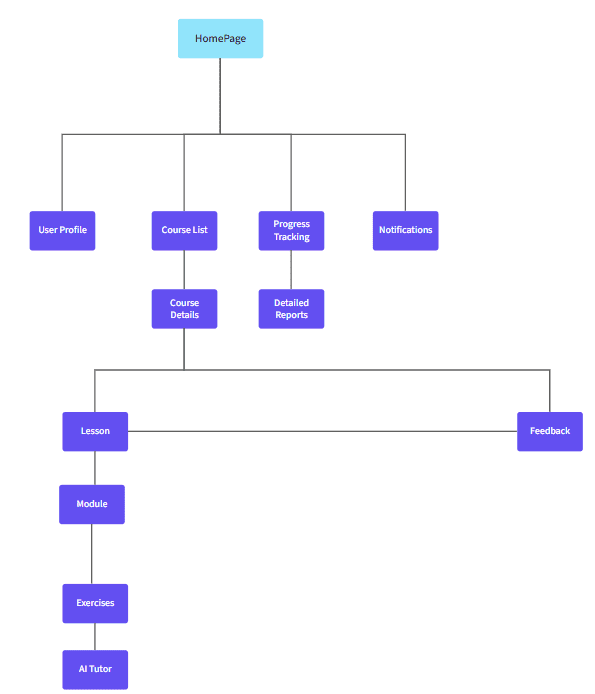
\includegraphics[scale=0.8]{Images/sitemap/Student.png}
    \caption{Sitemap cho đối tượng Sinh viên}
    \label{fig:enter-label}
\end{figure}
\par Sơ đồ trang web này thể hiện cấu trúc tổng thể của ứng dụng web, hiển thị các trang chính và mối quan hệ giữa chúng, đặc biệt là đối với đối tượng người dùng \textbf{Sinh viên}. Ở phía trên, có "Landing Page", "Log In Page" và "Dashboard Page". Đây là các trang điều hướng chính cho người dùng.
\par Bên dưới, có một số phần khác:

\begin{itemize}
    \item \textbf{User Profile:} Phần này chứa các trang liên quan đến tài khoản, thông tin cá nhân và cài đặt của sinh viên.
    \item \textbf{Course List Page:} Trang này hiển thị danh sách các khóa học mà sinh viên có thể truy cập.
    \item \textbf{Progress Tracking Page:} Trang này cho phép sinh viên theo dõi tiến độ và hiệu suất của họ trong các khóa học.
    \item \textbf{Notifications:} Phần này bao gồm trang chứa các thông báo cho sinh viên các cập nhật, tin nhắn hoặc cảnh báo quan trọng.
    \item \textbf{Course Detail Page:} Trang này cung cấp thông tin chi tiết về một khóa học cụ thể, như nội dung, mục tiêu và các tài nguyên khác.
    \item \textbf{Detailed Recommendation Lesson:} Trang này cung cấp các khóa học đề xuất học tập dựa trên tiến độ và mong muốn của người dùng.
    \item \textbf{Module Learning (Quiz), Module Learning (Code Exercises), and Module Learning (Reading Material):} Những phần này đại diện cho nội dung module của các bài học được đề xuất và chia thành 3 dạng bài tập như bài kiểm tra dạng quiz (multiple choices), bài tập lập trình thực hành và tài liệu đọc.
\end{itemize}
\par Nhìn chung, sơ đồ trang web này hiển thị các trang của hệ thống của đối tượng người dùng \textbf{Sinh viên} và cung cấp một cái nhìn tổng quan về cách các trang và chức năng liên quan được tổ chức và tương tác với nhau.
\subsubsection{Giảng viên}
\begin{figure}[H]
    \centering
    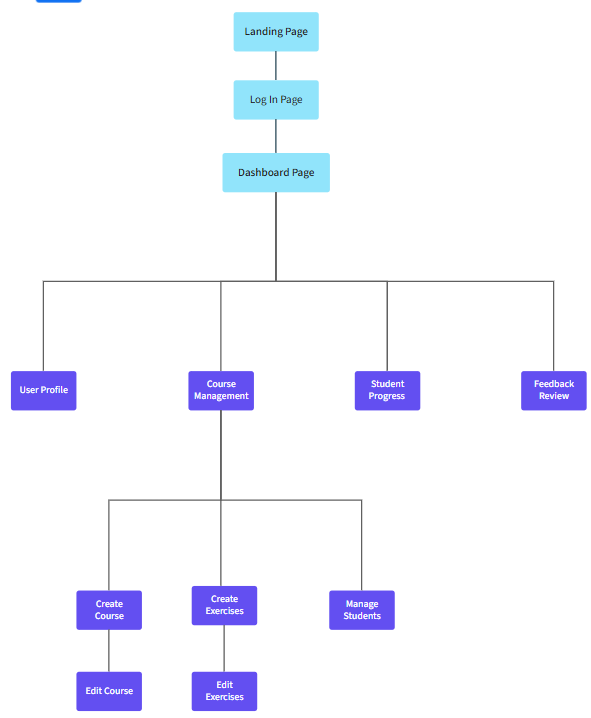
\includegraphics[scale=0.7]{Images/sitemap/Instructor.png}
    \caption{Sitemap cho đối tượng Giảng viên}
    \label{fig:enter-label}
\end{figure}
\par Sơ đồ trang web này đại diện cho cấu trúc của ứng dụng web, tập trung vào các chức năng và trang dành riêng cho giảng viên.

\par Ở phía trên, vẫn có các trang điều hướng chính như "Landing Page", "Log In Page" và "Dashboard Page", giúp giảng viên dễ dàng truy cập vào các phần quan trọng của hệ thống.

\par Bên dưới, sơ đồ được chia thành bốn phần chính:

\begin{itemize}
    \item \textbf{User Profile (Hồ sơ người dùng)}: Phần này chứa các trang liên quan đến thông tin cá nhân, tài khoản và cài đặt của giảng viên. Giảng viên có thể cập nhật thông tin cá nhân và quản lý các tùy chọn hệ thống của mình.
    \item \textbf{Course Management (Quản lý khóa học)}: Đây là phần quan trọng nhất với giảng viên, bao gồm các trang để tạo, chỉnh sửa, và quản lý các khóa học mà họ giảng dạy. Giảng viên có thể thêm các bài giảng, tài liệu học, và bài kiểm tra cho sinh viên.
    \item \textbf{Student Progress (Tiến độ học sinh)}: Phần này giúp giảng viên theo dõi và giám sát tiến độ học tập của sinh viên trong các khóa học mà họ giảng dạy. Giảng viên có thể xem thông tin về kết quả học tập của sinh viên, bao gồm điểm kiểm tra, bài tập và các hoạt động học tập khác.
    \item \textbf{Feedback Management (Quản lý phản hồi)}: Phần này cho phép giảng viên thu thập, quản lý và phân tích phản hồi từ sinh viên về khóa học, bài giảng, hoặc các hoạt động học tập. Đây là công cụ hữu ích để giảng viên đánh giá mức độ hiệu quả của phương pháp giảng dạy và cải thiện chất lượng khóa học.
\end{itemize}

\par Các trang con trong mỗi phần cung cấp các chức năng cụ thể hơn, chẳng hạn như chỉnh sửa nội dung khóa học, xem bảng điểm và thông tin phản hồi từ sinh viên.

\par \textbf{Tổng quan:} Sơ đồ trang web này cung cấp cái nhìn tổng quát về các chức năng chính mà giảng viên cần để quản lý khóa học, theo dõi tiến độ sinh viên và thu thập phản hồi. Cấu trúc đơn giản, dễ sử dụng, giúp giảng viên dễ dàng thực hiện các công việc quản lý và giảng dạy hiệu quả.
\subsubsection{Manager}
\begin{figure}[H]
    \centering
    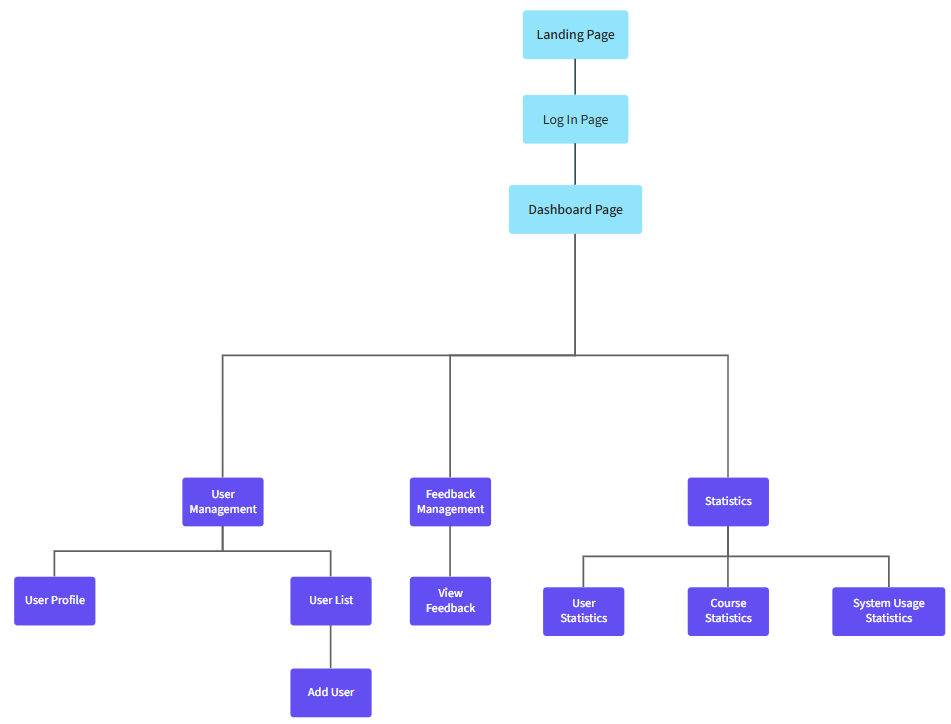
\includegraphics[scale=0.55]{Images/sitemap/Manager.png}
    \caption{Sitemap cho đối tượng Quản trị viên}
    \label{fig:enter-label}
\end{figure}
\par Sơ đồ trang web này cung cấp cái nhìn tổng quát về các chức năng chính mà Admin cần để quản lý các chức năng người dùng.

\par Ở phía trên, các trang điều hướng chính vẫn là "Landing Page", "Log In Page", và "Dashboard Page".

\par Các phần chính trong sơ đồ trang web này là:

\begin{itemize}
    \item \textbf{User Management:} Phần này bao gồm các trang để quản lý hồ sơ cá nhân, cài đặt và thông tin tài khoản của người dùng.
    \item \textbf{Feedback Management:} Phần này tập trung vào các trang để cung cấp phản hồi, đánh giá và nhận xét liên quan đến trải nghiệm học tập của người dùng.
    \item \textbf{Statistics:} Phần này cung cấp các trang hiển thị các số liệu thống kê, chỉ số và dữ liệu liên quan đến tiến độ, hiệu suất và mức độ sử dụng hệ thống của người dùng.
\end{itemize}

\par Các trang cấp thấp hơn trong sơ đồ trang web này hướng đến học sinh, chẳng hạn như các trang để xem chi tiết khóa học, truy cập tài liệu học tập và theo dõi tiến độ cá nhân.

\par Sơ đồ trang web này gợi ý về một ứng dụng web được thiết kế để cung cấp cho học sinh một trải nghiệm học tập cá nhân hóa, với sự tập trung vào quản lý người dùng, phản hồi và các thông tin chi tiết dựa trên dữ liệu để hỗ trợ hành trình giáo dục của họ.
\section*{Tổng kết}

Nhìn chung, ba sơ đồ trang web này thể hiện các góc nhìn và ưu tiên khác nhau trong thiết kế và chức năng của ứng dụng web, đáp ứng nhu cầu của các loại người dùng khác nhau, chẳng hạn như học sinh, giảng viên và quản trị viên.


\section{Quy trình Đề xuất và Theo dõi Lộ trình Học tập Cá nhân hóa}

\subsection{Tổng quan}
Hệ thống học tập trực tuyến thông minh được thiết kế để cung cấp trải nghiệm học tập cá nhân hóa, hỗ trợ học viên đạt được mục tiêu học tập một cách hiệu quả. Quy trình tận dụng trí tuệ nhân tạo (AI) để phân tích nhu cầu học viên, đề xuất nội dung phù hợp, đánh giá tiến độ, và điều chỉnh lộ trình học tập khi cần. Các chức năng chính bao gồm xây dựng lộ trình học tập, tạo bài kiểm tra tự động, theo dõi hiệu quả học tập, và tạo bổ sung nội dung để giải quyết khó khăn.

Quy trình được chia thành bốn giai đoạn chính:
\begin{itemize}
	\item Phân tích mục tiêu và tạo lộ trình học tập.
	\item Tạo bài kiểm tra tự động.
	\item Theo dõi và đánh giá tiến độ học tập.
	\item Điều chỉnh nội dung học tập dựa trên kết quả học tập.
\end{itemize}

\subsection{Giai đoạn 1: Phân tích Mục tiêu và Tạo Lộ trình Học tập}
Giai đoạn này tập trung vào việc hiểu mục tiêu học tập của học viên và xây dựng một kế hoạch học tập phù hợp, sử dụng AI để phân tích và đề xuất nội dung.

\begin{enumerate}
	\item \textbf{Hiểu mục tiêu học tập}: Hệ thống thu thập mục tiêu của học viên, ví dụ: ``nắm vững lập trình Python cơ bản'' hoặc ``cải thiện kỹ năng giải thuật''. AI phân tích mục tiêu để đảm bảo nó rõ ràng, phù hợp với khóa học, và khả thi trong thời gian quy định. Nếu mục tiêu có thời hạn cụ thể (như trước kỳ thi giữa kỳ), hệ thống xác định khoảng thời gian phù hợp.

	\item \textbf{Prompt sử dụng}:
	      \begin{Verbatim}[breaklines=true]
		      Phân tích mục tiêu học tập: "[goal]". Xác định tính hoàn chỉnh, phù hợp với khóa học "[course_name]", và khả thi dựa trên kết quả học tập mong đợi. Đề xuất dòng thời gian từ [start_date] đến [end_date]. Trả về JSON với start_date, end_date, và ghi chú xác thực.
	      \end{Verbatim}
	      Prompt này yêu cầu AI kiểm tra tính hợp lệ của mục tiêu và đề xuất thời gian thực hiện, đảm bảo lộ trình học tập phù hợp với lịch trình khóa học.

	\item \textbf{Lựa chọn bài học phù hợp}: AI xem xét nội dung khóa học và chọn các bài học liên quan nhất đến mục tiêu. Các bài học được sắp xếp từ cơ bản đến nâng cao, kèm theo giải thích về lý do lựa chọn, giúp học viên dễ dàng tiếp cận kiến thức.

	\item \textbf{Prompt sử dụng}:
	      \begin{Verbatim}[breaklines=true]
		      Dựa trên mục tiêu "[goal]" và khóa học "[course_name]", chọn các bài học từ danh sách [lessons_data]. Sắp xếp theo thứ tự logic, ưu tiên bài học cơ bản nếu thời gian ngắn. Trả về danh sách bài học với ID, thứ tự, tiêu đề, và lý do chọn.
	      \end{Verbatim}
	      Prompt này hướng dẫn AI lọc và sắp xếp bài học dựa trên mục tiêu, đảm bảo tính liên quan và trình tự hợp lý.

	\item \textbf{Xây dựng lộ trình chi tiết}: Hệ thống tạo lộ trình học tập bao gồm các bài học được chia thành các phần nhỏ (module), mỗi phần có nội dung lý thuyết, hướng dẫn thực hành, và tài liệu tham khảo. AI thiết kế lộ trình phù hợp với thời gian và tốc độ học của học viên.

	\item \textbf{Prompt sử dụng}:
	      \begin{Verbatim}[breaklines=true]
		      Tạo lộ trình học tập cho mục tiêu "[goal]" từ [start_date] đến [end_date]. Dựa trên bài học [selected_lessons], tạo danh sách bài học đề xuất với nội dung trọng tâm, giải thích lý do, và 2-3 module mỗi bài học. Trả về JSON với bài học và module chi tiết.
	      \end{Verbatim}
	      Prompt này yêu cầu AI tạo lộ trình chi tiết, bao gồm nội dung và module, để hỗ trợ học viên đạt mục tiêu một cách có hệ thống.
\end{enumerate}

\subsection{Giai đoạn 2: Tạo Bài Kiểm tra Tự động}
Hệ thống sử dụng AI để tạo bài kiểm tra nhằm đánh giá sự hiểu biết của học viên dựa trên nội dung học tập.

\begin{enumerate}
	\item \textbf{Xác định nội dung kiểm tra}: Hệ thống chọn một phần nội dung cụ thể (module) để tạo bài kiểm tra, tập trung vào các khái niệm và kỹ năng quan trọng.

	\item \textbf{Tạo câu hỏi đa dạng}: AI tạo các câu hỏi với nhiều mức độ khó (dễ, trung bình, khó) và loại hình (trắc nghiệm đơn, đa lựa chọn, đúng/sai). Mỗi câu hỏi đi kèm giải thích chi tiết để học viên hiểu rõ đáp án.

	\item \textbf{Prompt sử dụng}:
	      \begin{Verbatim}[breaklines=true]
		      Tạo [count] câu hỏi [difficulty] cho module "[module_title]". Câu hỏi dựa trên mục tiêu [objectives] và nội dung "[recommended_content]". Bao gồm loại câu hỏi đa dạng (single_choice, multiple_choice, true_false), với giải thích chi tiết. Trả về JSON với câu hỏi, lựa chọn, đáp án, và điểm.
	      \end{Verbatim}
	      Prompt này chỉ đạo AI tạo câu hỏi phù hợp với nội dung module, đảm bảo đa dạng và có giá trị đánh giá cao.

	\item \textbf{Thiết lập thông tin bài kiểm tra}: Hệ thống đặt thời gian làm bài và tổng điểm dựa trên số lượng câu hỏi, đảm bảo bài kiểm tra cân đối và khả thi.

	\item \textbf{Prompt sử dụng}:
	      \begin{Verbatim}[breaklines=true]
		      Thiết lập bài kiểm tra cho module "[module_title]". Dựa trên [questions_count] câu hỏi, tính thời gian làm bài (2 phút/câu, tối đa 60 phút) và tổng điểm. Trả về JSON với tên, mô tả, thời gian, và điểm tối đa.
	      \end{Verbatim}
	      Prompt này giúp AI cấu hình bài kiểm tra phù hợp với khối lượng nội dung, đảm bảo trải nghiệm học tập công bằng.
\end{enumerate}

\subsection{Giai đoạn 3: Theo dõi và Đánh giá Tiến độ Học tập}
Hệ thống liên tục theo dõi quá trình học tập của học viên, sử dụng AI để đánh giá và đưa ra gợi ý cải thiện.

\begin{enumerate}
	\item \textbf{Thu thập dữ liệu học tập}: Hệ thống ghi nhận thời gian học, tiến độ hoàn thành bài học, và kết quả bài kiểm tra, từ đó đánh giá mức độ nỗ lực và hiểu biết của học viên.

	\item \textbf{Đánh giá theo tiêu chí}: AI phân tích tiến độ dựa trên ba yếu tố:
	      \begin{itemize}
		      \item \textit{Kiến thức lý thuyết}: Mức độ hiểu các khái niệm quan trọng.
		      \item \textit{Kỹ năng thực hành}: Khả năng áp dụng kiến thức, như viết mã lập trình.
		      \item \textit{Mức độ nỗ lực}: Sự chăm chỉ, dựa trên thời gian học và số bài học đã bắt đầu.
	      \end{itemize}

	\item \textbf{Prompt sử dụng}:
	      \begin{Verbatim}[breaklines=true]
		      Đánh giá tiến độ học viên "[student_name]" với mục tiêu "[goal]". Dựa trên dữ liệu bài học [lessons_data], phân tích theo kiến thức lý thuyết, kỹ năng thực hành, và nỗ lực. Trả về JSON với báo cáo STAR, điểm mạnh, điểm cần cải thiện, và gợi ý chi tiết.
	      \end{Verbatim}
	      Prompt này yêu cầu AI tạo báo cáo toàn diện, giúp học viên hiểu rõ tình trạng học tập và nhận gợi ý cụ thể.

	\item \textbf{Báo cáo chi tiết}: AI tạo báo cáo nêu rõ điểm mạnh (như nắm vững lý thuyết), điểm cần cải thiện (như kỹ năng thực hành còn yếu), và gợi ý (như tập trung vào bài tập thực hành). Báo cáo được trình bày rõ ràng để học viên dễ áp dụng.
\end{enumerate}

\subsection{Giai đoạn 4: Điều chỉnh Nội dung Học tập}
Khi học viên gặp khó khăn, hệ thống sử dụng AI để phân tích và tái tạo nội dung học tập, giúp giải quyết vấn đề hiệu quả.

\begin{enumerate}
	\item \textbf{Phân tích vấn đề}: AI xem xét các khó khăn, như hiểu sai khái niệm hoặc mắc lỗi thực hành, và xác định liệu học viên cần ôn lại nội dung trước đó.

	\item \textbf{Prompt sử dụng}:
	      \begin{Verbatim}[breaklines=true]
		      Phân tích vấn đề từ dữ liệu [issues_summary] cho bài học "[lesson_title]". Xác định các khó khăn chính (hiểu sai, lỗi thực hành) và đề xuất hành động (lặp lại, xem lại bài trước). Trả về JSON với danh sách vấn đề, mức độ nghiêm trọng, và hành động đề xuất.
	      \end{Verbatim}
	      Prompt này giúp AI xác định nguyên nhân khó khăn và đề xuất cách khắc phục phù hợp.

	\item \textbf{Tái tạo nội dung}: AI tạo lại nội dung bài học, tập trung vào giải quyết các vấn đề đã xác định. Nội dung mới bao gồm ví dụ thực tế, hướng dẫn chi tiết, và tài liệu tham khảo phù hợp.

	\item \textbf{Prompt sử dụng}:
	      \begin{Verbatim}[breaklines=true]
		      Tái tạo nội dung cho bài học "[lesson_title]" dựa trên vấn đề [issues_analysis]. Cung cấp nội dung mới với giải thích chi tiết, ví dụ thực tế, và 2-3 module tập trung vào khó khăn. Trả về JSON với nội dung đề xuất, giải thích, và module.
	      \end{Verbatim}
	      Prompt này chỉ đạo AI thiết kế nội dung mới, đảm bảo phù hợp với nhu cầu cụ thể của học viên.

	\item \textbf{Cập nhật lộ trình}: Nội dung mới được tích hợp vào lộ trình học tập, giúp học viên tiếp tục học mà không bị gián đoạn.
\end{enumerate}

\subsection{Kết luận}
Quy trình đề xuất và theo dõi lộ trình học tập cá nhân hóa tận dụng trí tuệ nhân tạo để mang lại trải nghiệm học tập linh hoạt và hiệu quả. Các câu lệnh AI (prompt) được thiết kế cẩn thận để phân tích mục tiêu, tạo nội dung, đánh giá tiến độ, và điều chỉnh lộ trình, giúp học viên vượt qua khó khăn và đạt được mục tiêu học tập. Quy trình này không chỉ nâng cao chất lượng học tập mà còn đảm bảo sự hỗ trợ liên tục, phù hợp với từng cá nhân.

\section{Thiết kế giao diện}
\subsection{Landing Page}
\begin{figure}[H]
    \centering
    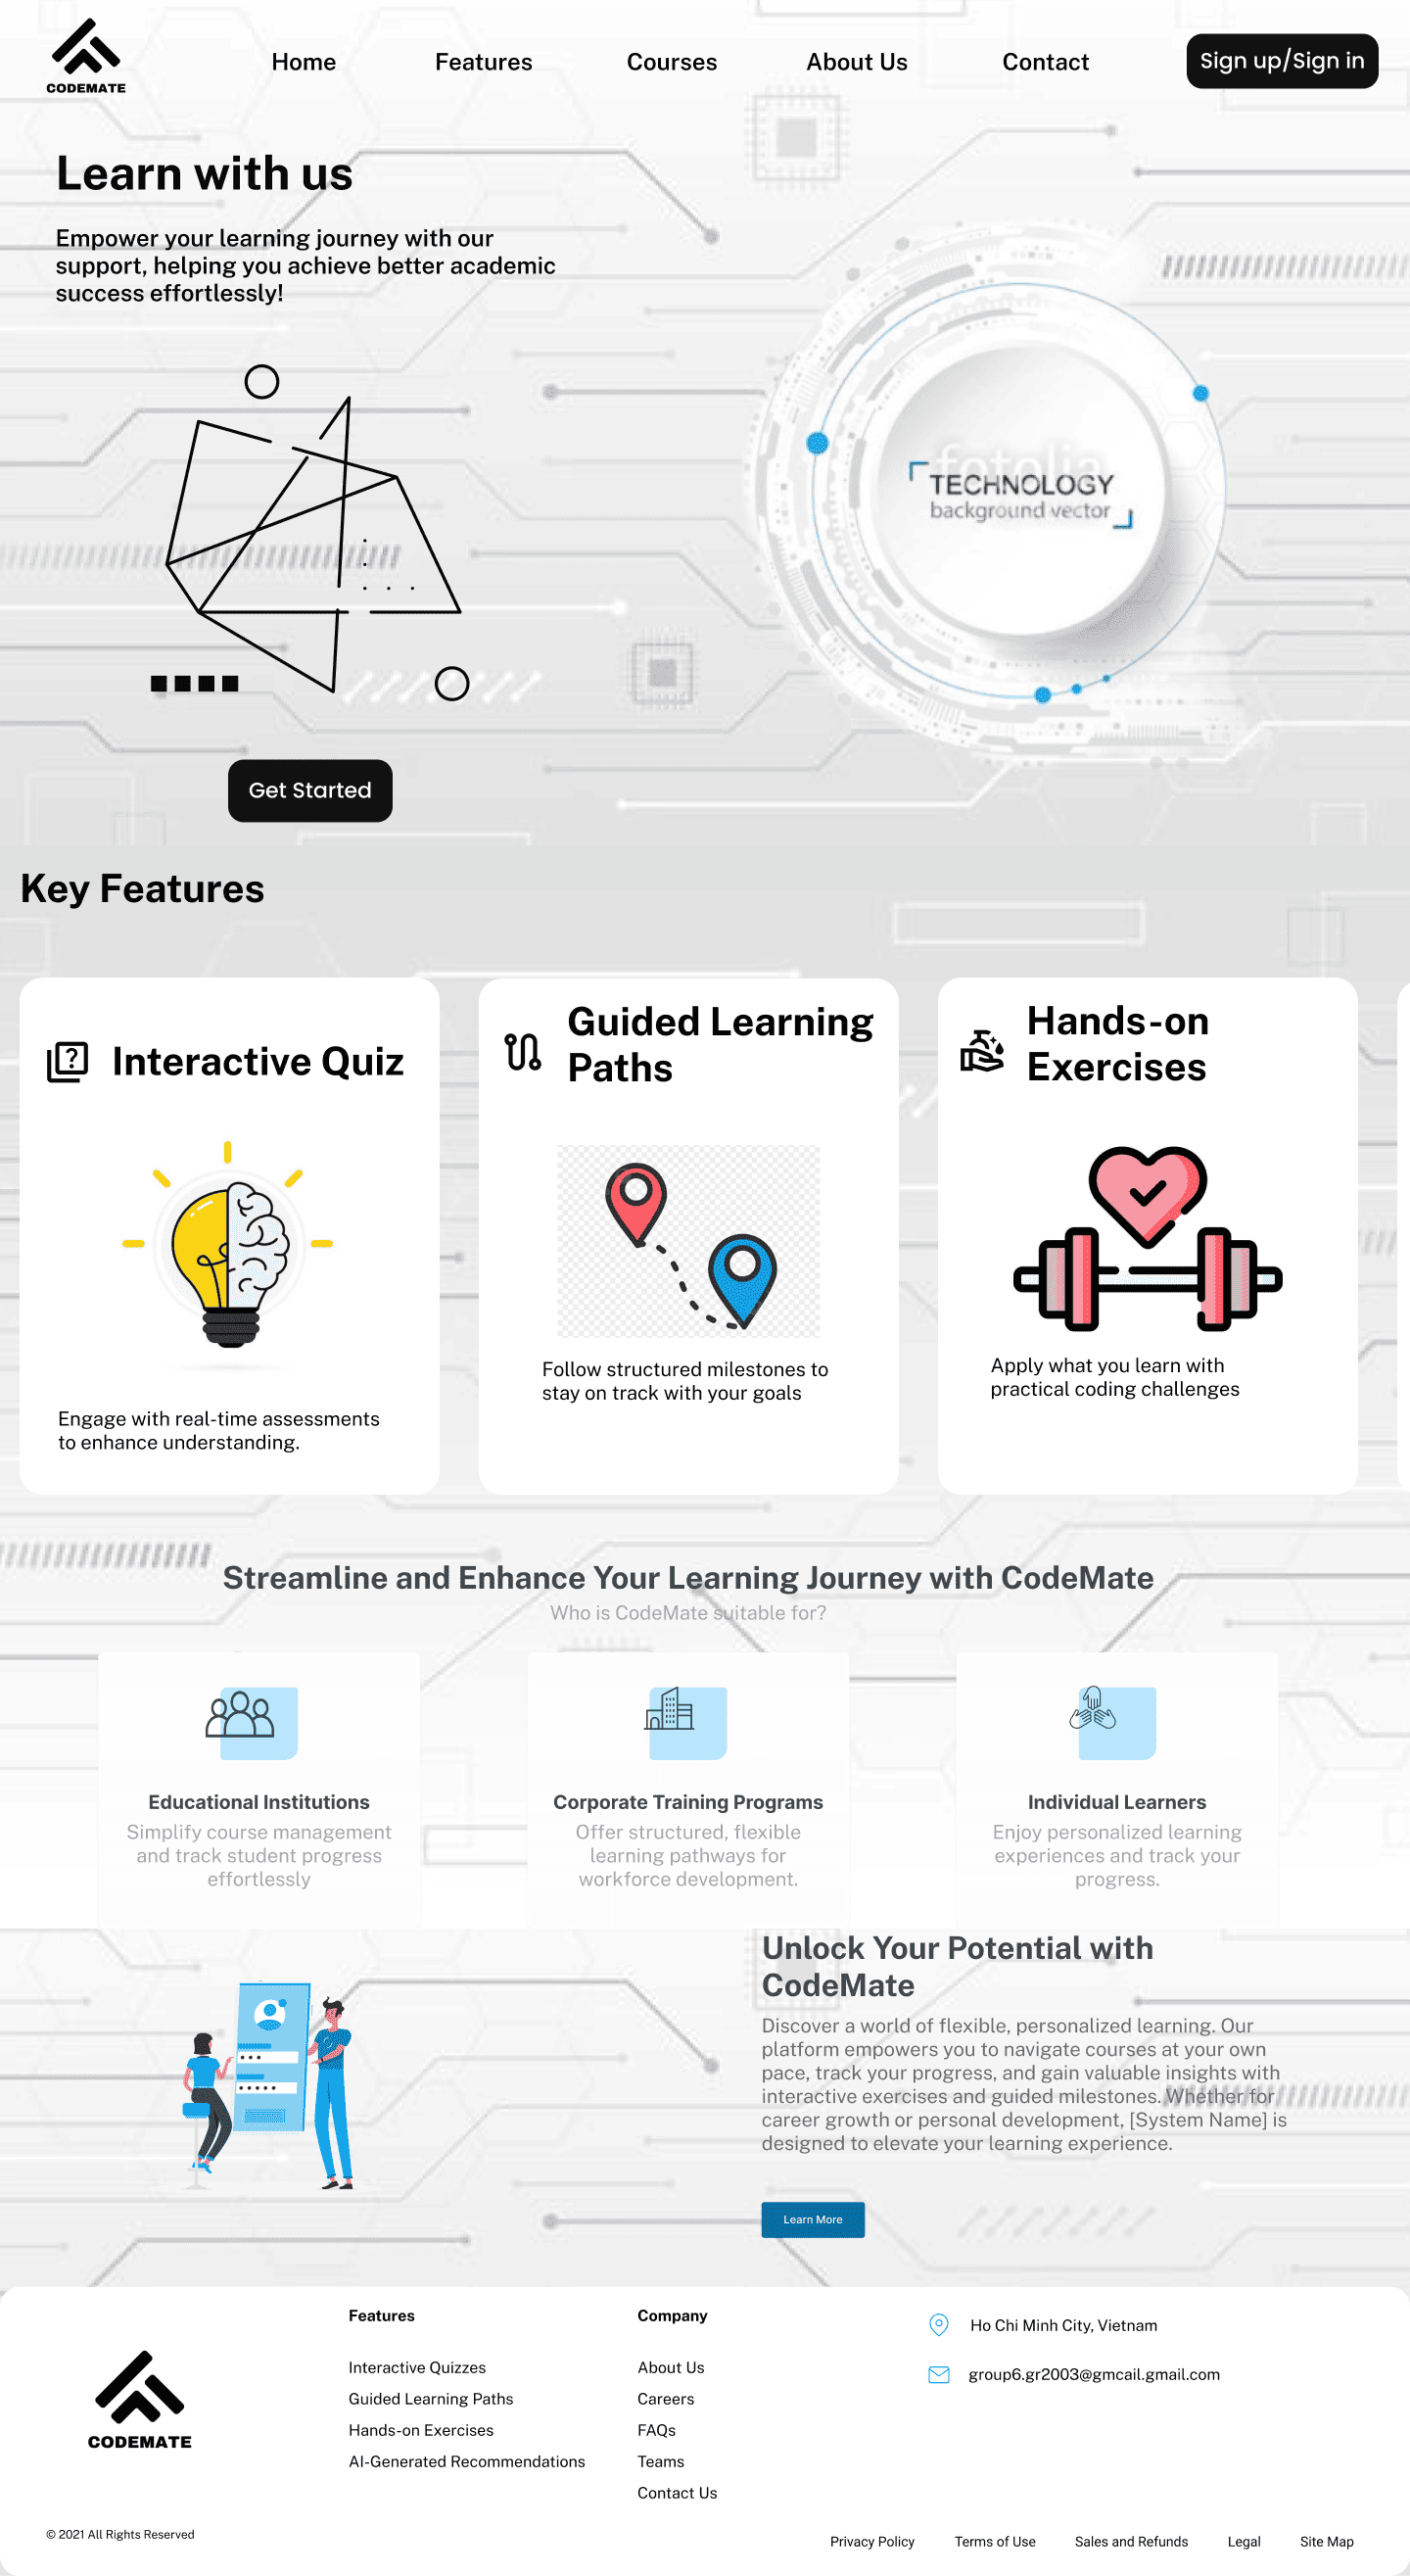
\includegraphics[width=0.7\linewidth]{Images/figmaDesign/Landing Page.png}
    \caption{Landing Page}
    \label{fig:enter-label}
\end{figure}
Landing Page mô tả tổng quát về website hỗ trợ học tập \textbf{\textit{CODEMATE}}.
\subsection{Authentication}
\subsubsection{Log In Screen}
\begin{figure}[H]
    \centering
    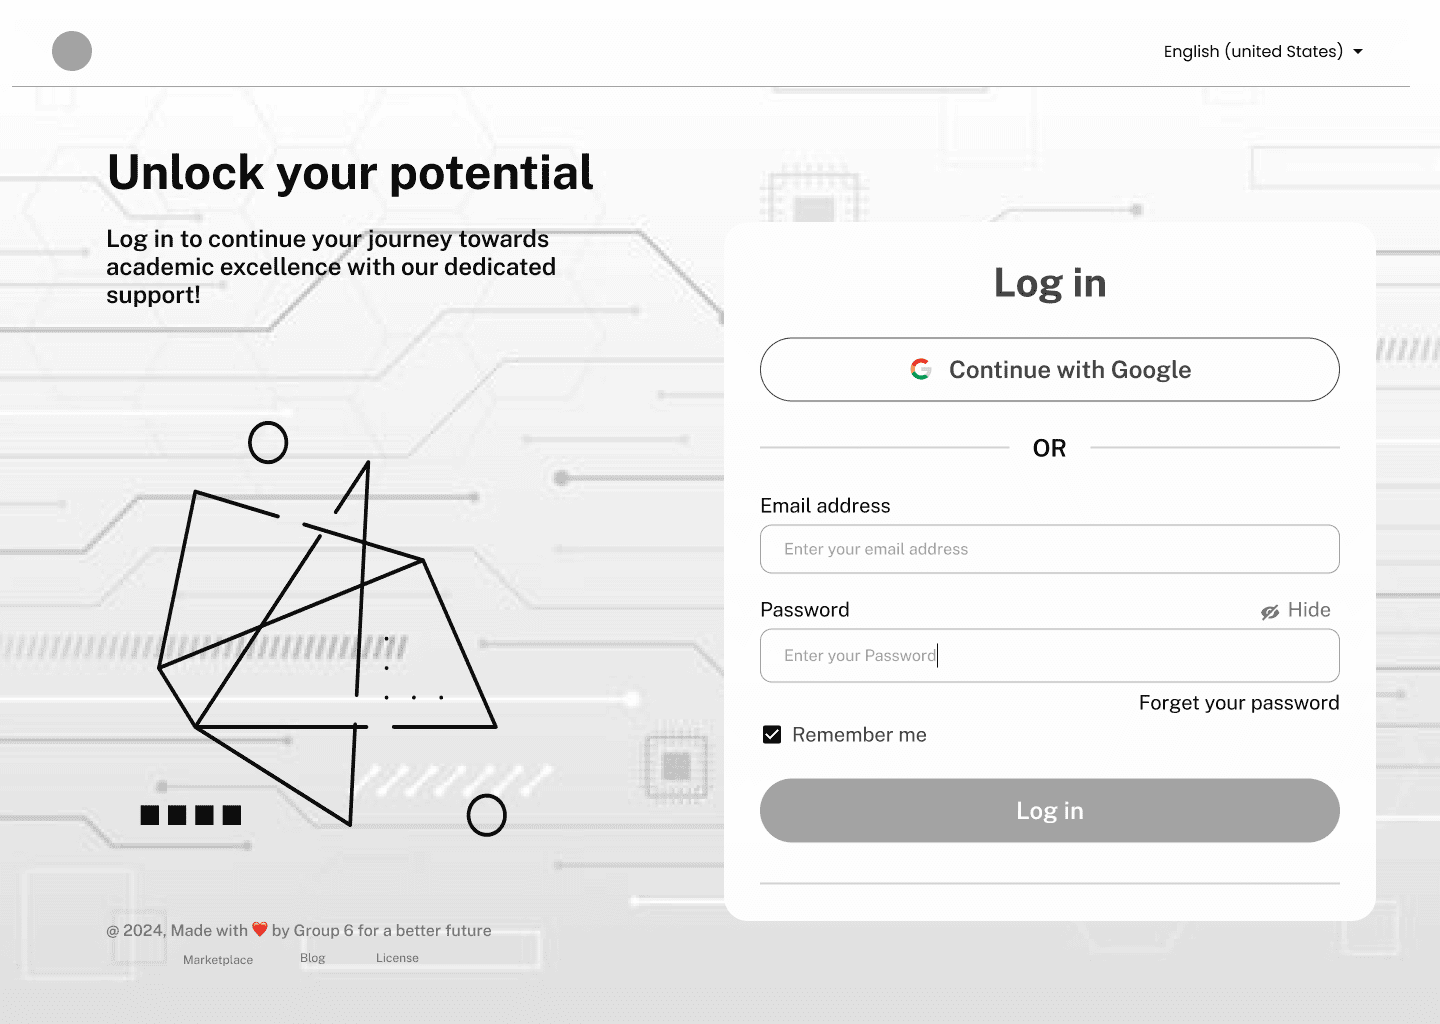
\includegraphics[width=0.7\linewidth]{Images/figmaDesign/Sign In Screen.png}
    \caption{Log In Screen}
    \label{fig:enter-label}
\end{figure}
Trang đăng nhập hệ thống, cho phép người dùng đăng nhập vào hệ thống bằng Email của mình hoặc qua phương thức đăng nhập bằng bên thứ ba \textbf{\textit{(Google)}}. Hệ thống sẽ nhận diện tên miền riêng của Email để xác định tính xác thực của Email trường Đại học do người dùng cung cấp. Nếu người dùng không dùng Email do trường Đại học cung cấp, sẽ không thể truy cập vào hệ thống. Ngoài ra, role của người dùng cũng sẽ được hệ thống phân loại dựa vào Email Address của người dùng và cơ sở dữ liệu của trường Đại học cung cấp cho hệ thống. 
\subsubsection{Forgot Password Screen}
\begin{figure}[H]
    \centering
    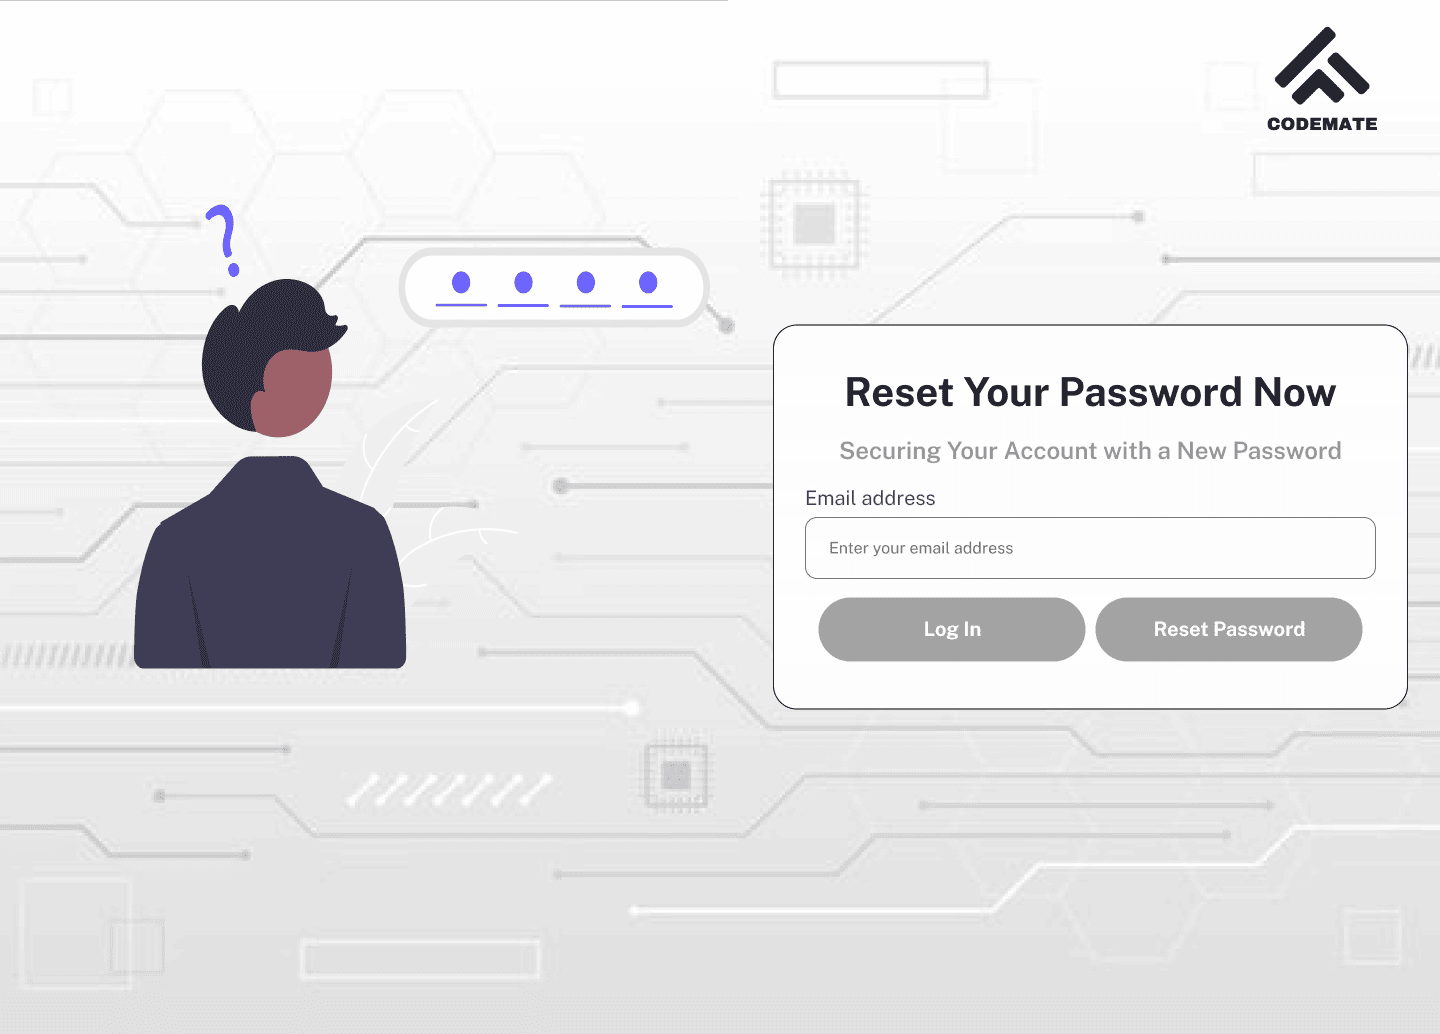
\includegraphics[width=0.7\linewidth]{Images/figmaDesign/Forgot Password Screen.png}
    \caption{Forgot Password Screen}
    \label{fig:enter-label}
\end{figure}
\subsubsection{Reset Password Screen}
\begin{figure}[H]
    \centering
    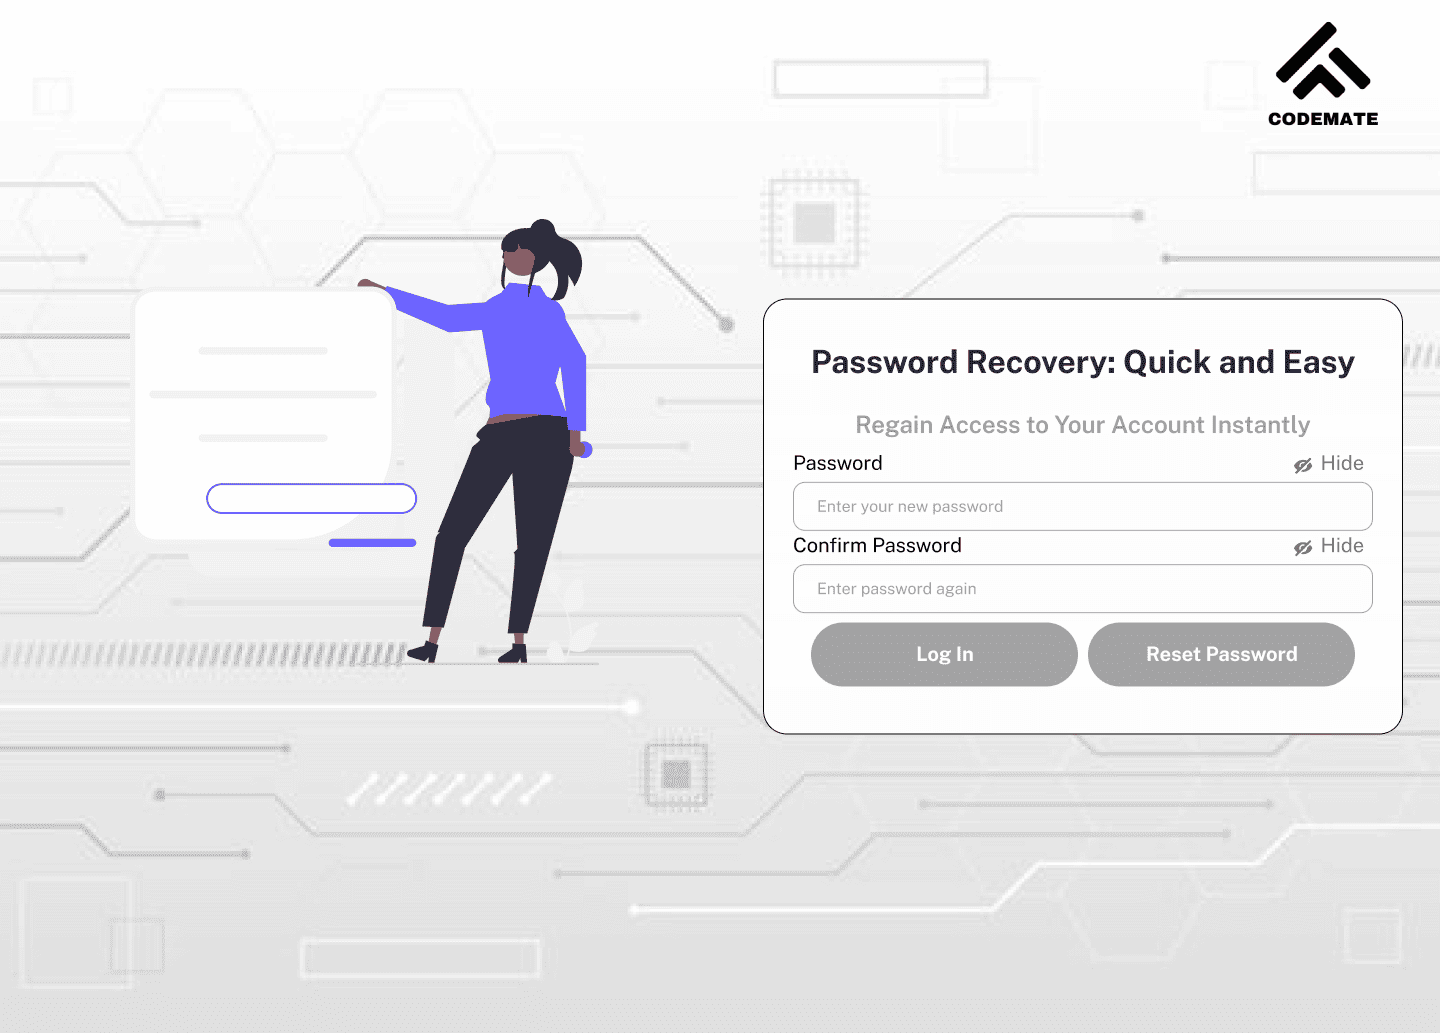
\includegraphics[width=0.7\linewidth]{Images/figmaDesign/Reset Password Screen.png}
    \caption{Reset Password Screen}
    \label{fig:enter-label}
\end{figure}
Các trang \textbf{\textit{"Forgot Password"}} và \textbf{\textit{"Reset Password"}} hỗ trợ người dùng trong trường hợp quên mật khẩu truy cập vào hệ thống và muốn lấy lại mật khẩu của mình thông qua địa chỉ Email. 
\subsection{Course Management (Student)}
\subsubsection{Courses List Screen}
\begin{figure}[H]
    \centering
    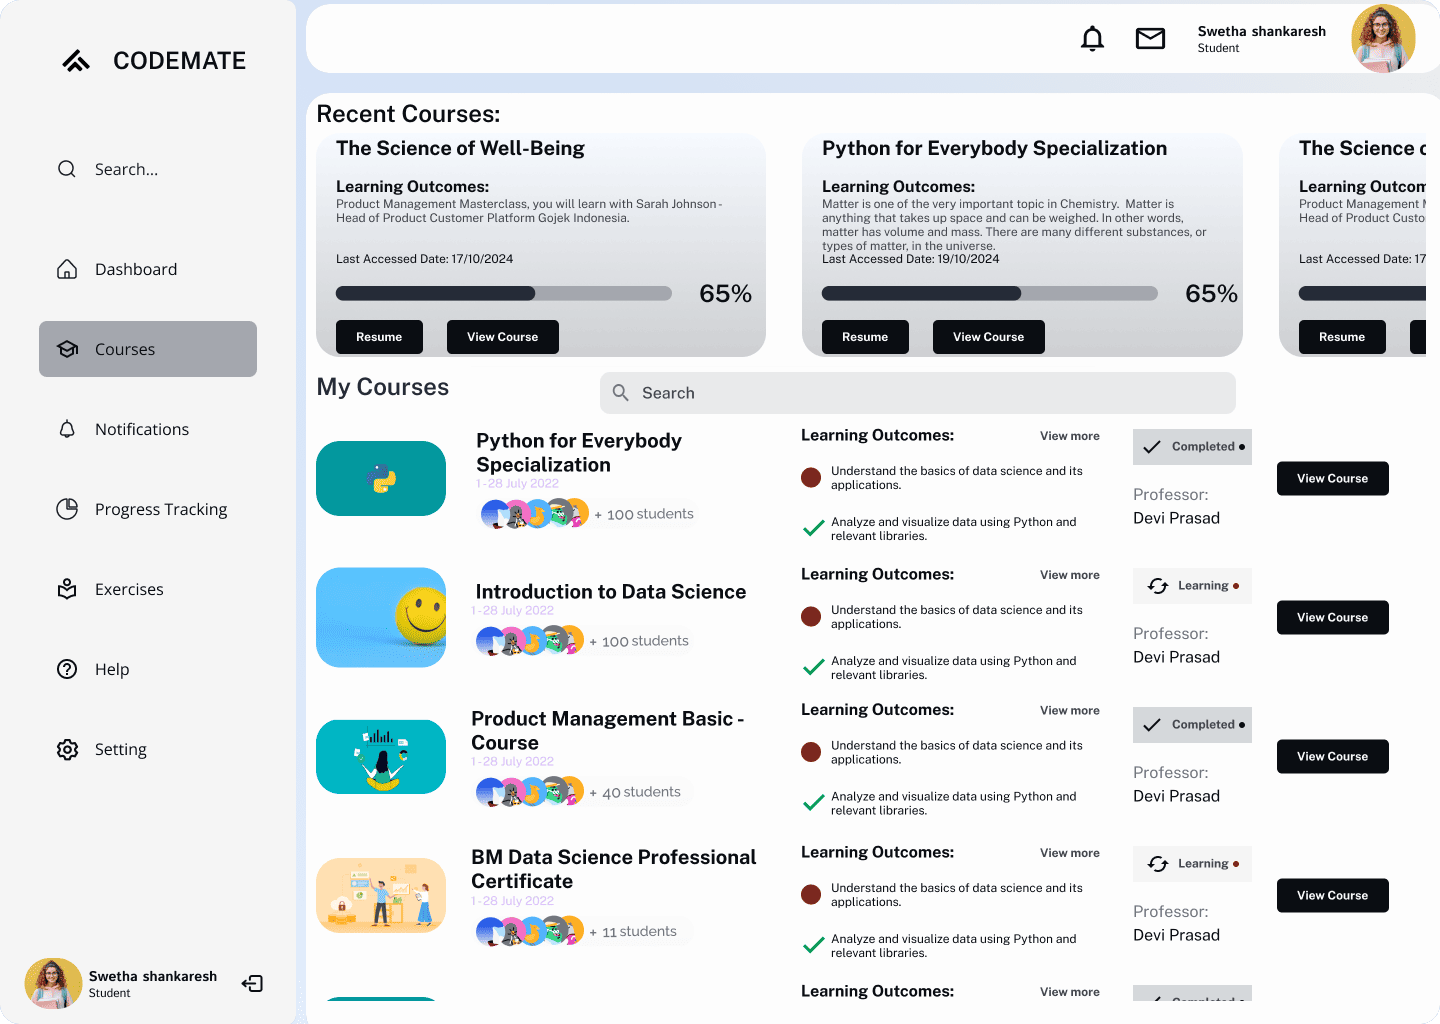
\includegraphics[width=0.7\linewidth]{Images/figmaDesign/Courses List Page.png}
    \caption{Courses List Screen}
    \label{fig:enter-label}
\end{figure}
Trang danh sách khóa học, hiển thị danh sách các khóa học mà sinh viên đã đăng ký tại học kỳ đó. Đặc biệt là các khóa học liên quan đến lĩnh vực \textbf{\textit{"Khoa học máy tính"}}. Sinh viên có thể xem các khóa học mình đã và đang học hoặc các khóa học truy cập gần đây. Mỗi khóa học hiển thị các thông tin như: \textbf{\textit{Tên khóa học, Tên giảng viên, Thời gian bắt đầu, Thời gian kết thúc, Đầu ra môn học}} và tác vụ \textbf{\textit{"Xem chi tiết khóa học"}}.
\begin{figure}[H]
    \centering
    
\includegraphics[width=0.7\linewidth]{Images/figmaDesign/Modal Learning Outcomes.png}
    \caption{Modal Learning Outcomes}
    \label{fig:enter-label}
\end{figure}
Sinh viên có thể xem chi tiết \textbf{\textit{"Đầu ra môn học"}} bằng nút \textbf{\textit{"View more"}}
\subsubsection{Detailed Course Screen}
Trang thông tin chi tiết khóa học, field Description, cho phép sinh viên xem mô tả \textbf{\textit{"Đầu ra môn học"}} do giảng viên cung cấp. Ngoài ra, các thông tin của khóa học như:\textbf{\textit{Tên môn học, Phần trăm hoàn thành hiện tại khóa học của sinh viên, Label trạng thái môn học, Số unit của khóa học, Tên giảng viên}} được hiển thị chung ở một component. Mỗi khóa học sẽ có 3 fields hỗ trợ cho các thông tin: \textbf{\textit{Description, Lessons, Exercises}}. 
\begin{figure}[H]
    \centering
    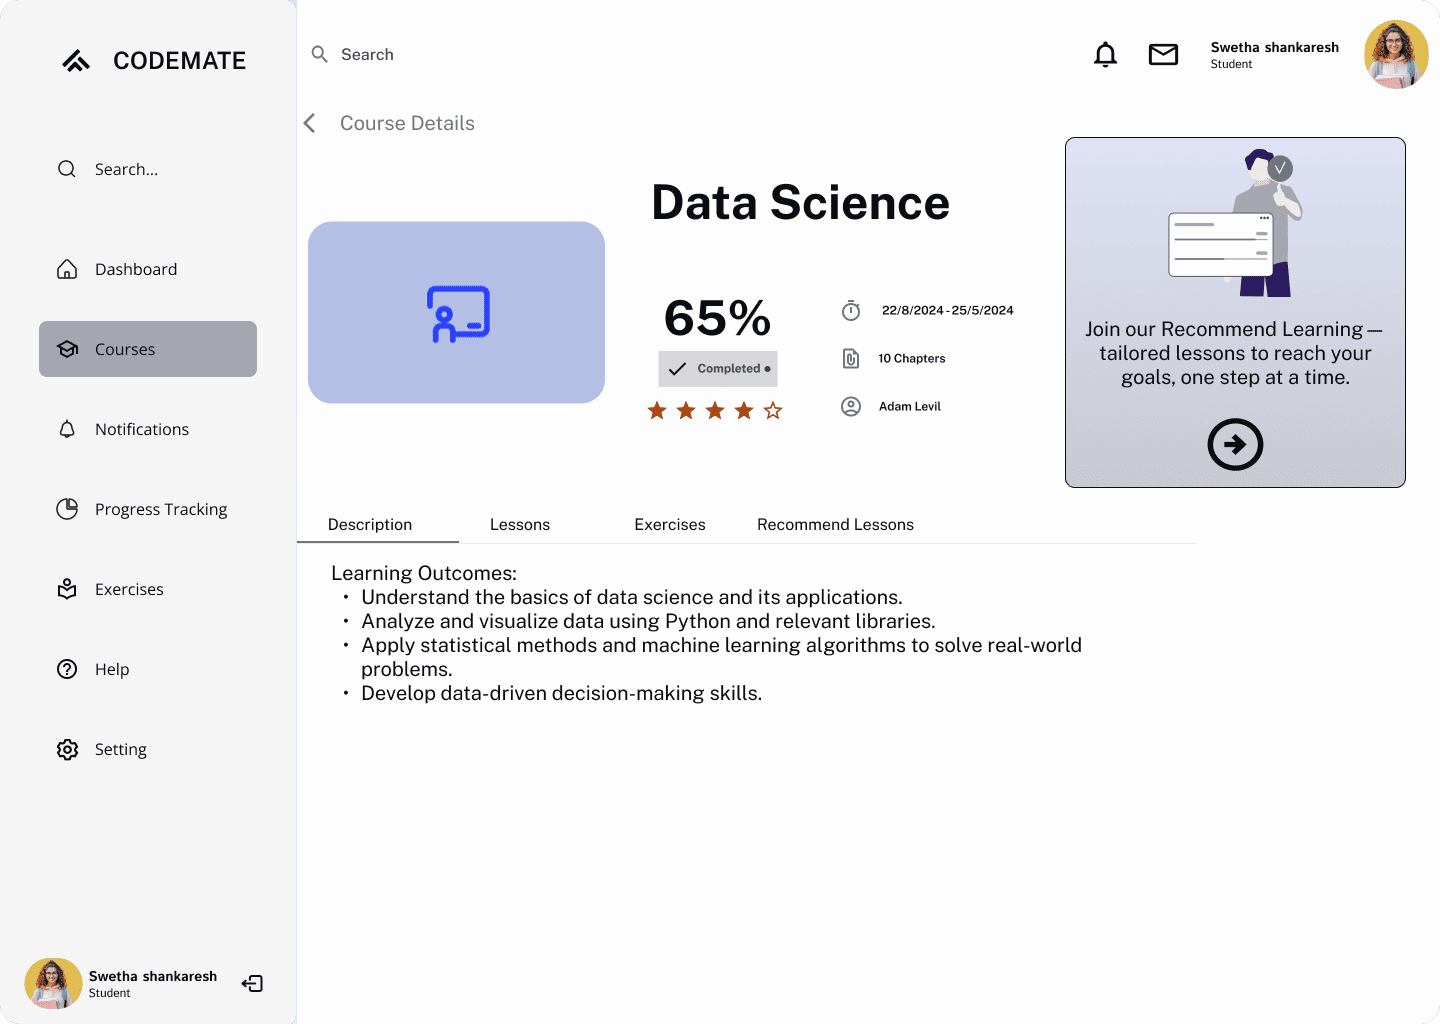
\includegraphics[width=0.7\linewidth]{Images/figmaDesign/Detailed Course Page - Description.png}
    \caption{Detailed Course Screen - Description}
    \label{fig:enter-label}
\end{figure}
Field Description chứa thông tin liên quan đến mô tả khóa học và đầu ra môn học do giảng viên cung cấp.
\begin{figure}[H]
    \centering
    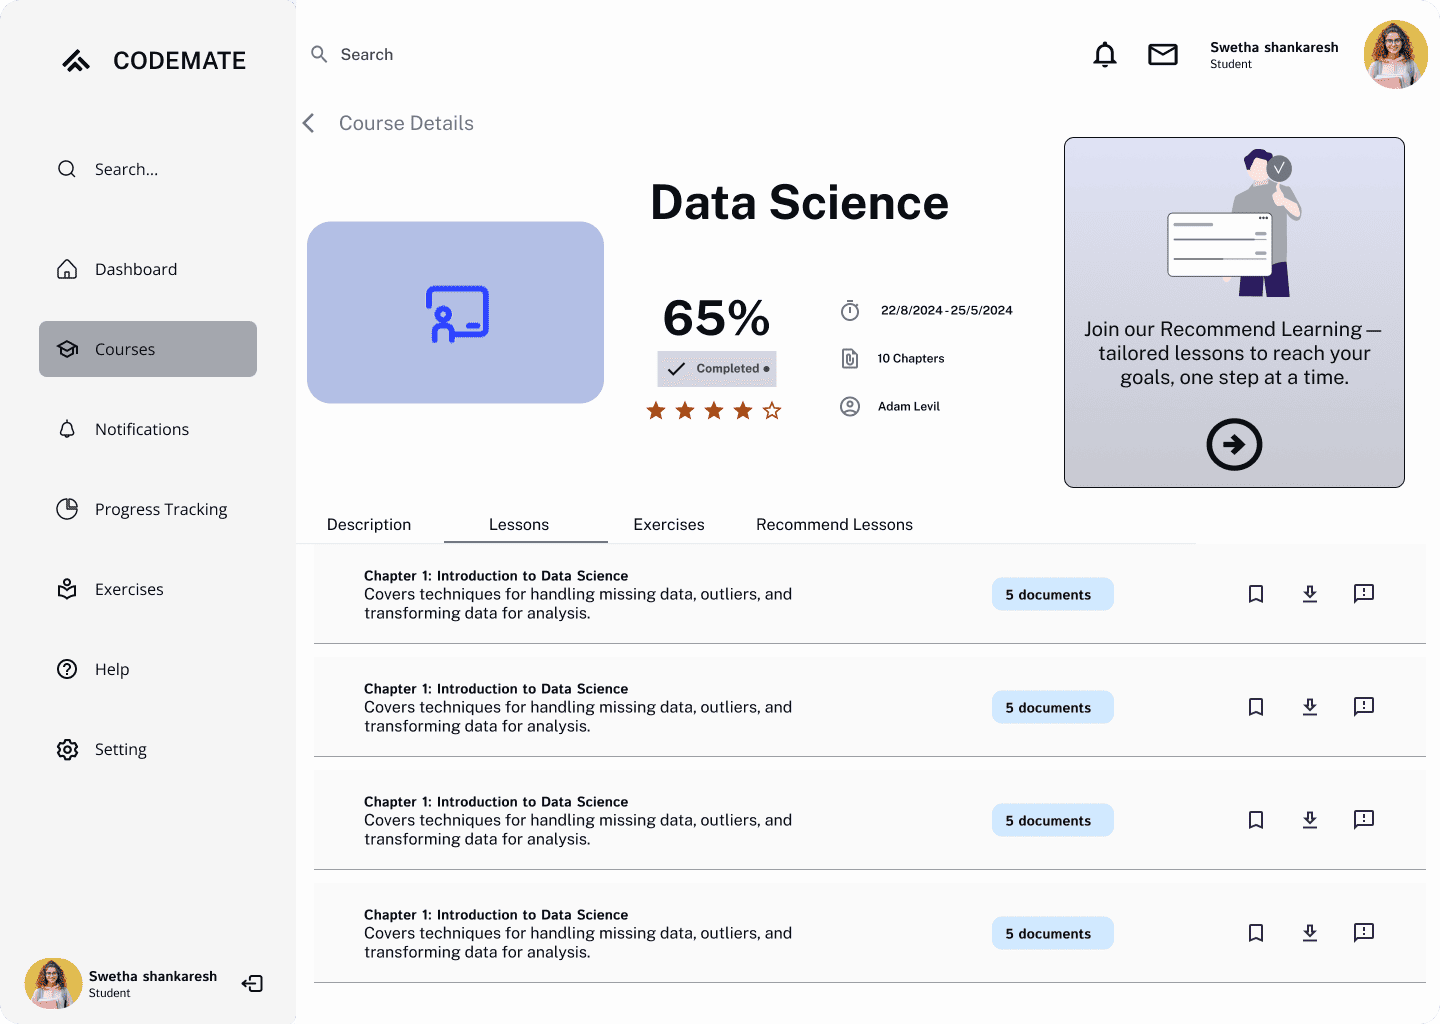
\includegraphics[width=0.7\linewidth]{Images/figmaDesign/Detailed Course Page - Lessons.png}
    \caption{Detailed Course Page - Lessons}
    \label{fig:enter-label}
\end{figure}
Field Lessons chứa các lessons được chia bởi giảng viên. Mỗi lesson được hiển thị với thông tin: \textbf{\textit{Tên lesson và Số tài liệu tham khảo được giảng viên đăng tải}}
\begin{figure}[H]
    \centering
    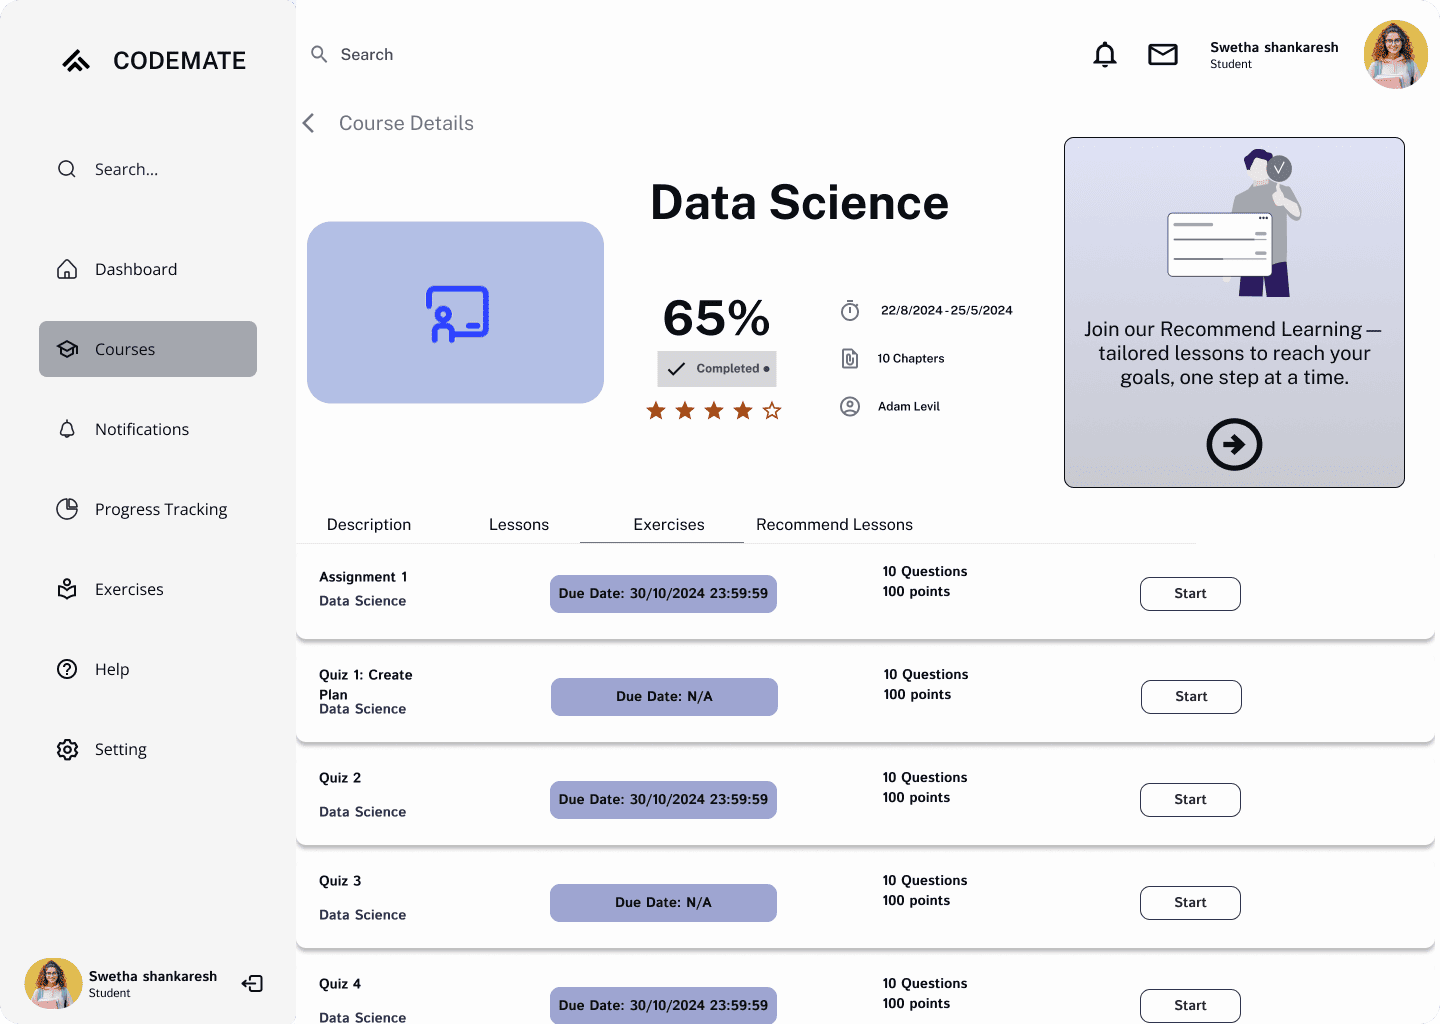
\includegraphics[width=0.7\linewidth]{Images/figmaDesign/Detailed Course Page - Exercises.png}
    \caption{Detailed Course Page - Exercises}
    \label{fig:enter-label}
\end{figure}
Field Exercises chứa các bài Quiz/Assignment do giảng viên hoặc hệ thống cung cấp hỗ trợ cho lesson/khóa học đó. 
\begin{figure}[H]
    \centering
    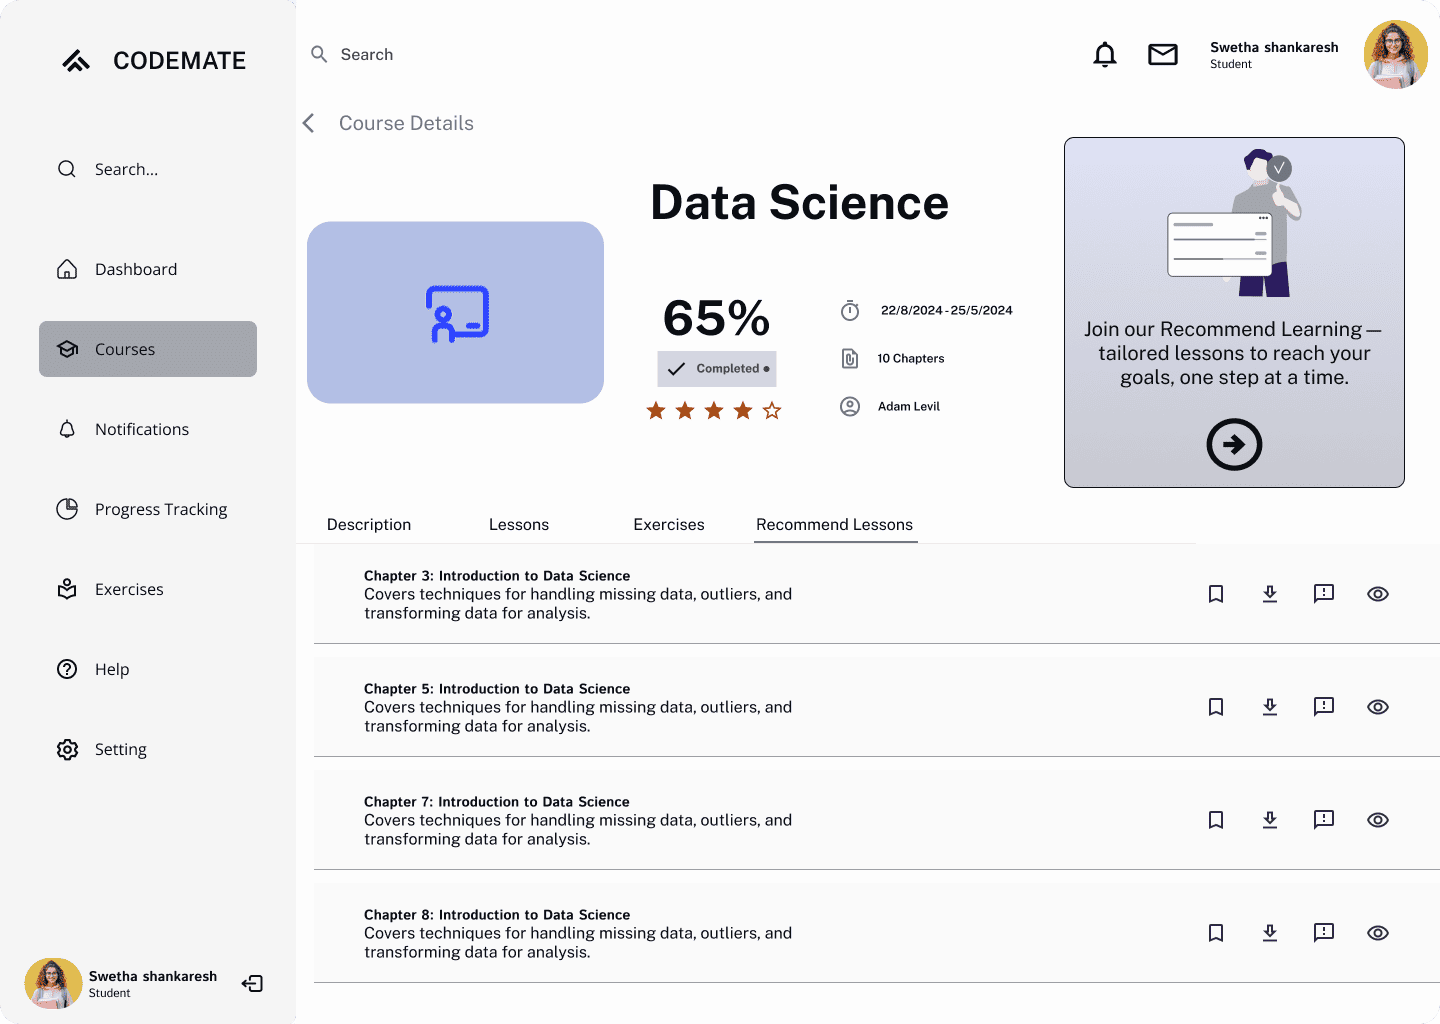
\includegraphics[width=0.7\linewidth]{Images/figmaDesign/Detailed Course Page - Recommend Lessons.png}
    \caption{Detailed Course Page - Recommend Lessons}
    \label{fig:enter-label}
\end{figure}
Field Recommend Lessons Chứa các lessons mà hệ thống đã đề xuất cho sinh viên. 
\subsubsection{Define Goal Modal}
\begin{figure}[H]
    \centering
    
\includegraphics[width=0.7\linewidth]{Images/figmaDesign/Get Goals Modal.png}
    \caption{Modal để lấy mục tiêu của sinh viên}
    \label{fig:enter-label}
\end{figure}
Sinh viên có thể cung cấp mục tiêu học tập của mình thông qua modal ở trang chi tiết khóa học
\subsubsection{Modules}
Sau khi chọn mục tiêu học tập và được hệ thống đề xuất lesson, sinh viên sẽ được truy cập vào lesson được đề xuất với giao diện chi tiết lesson như sau: 
\begin{figure}[H]
    \centering
    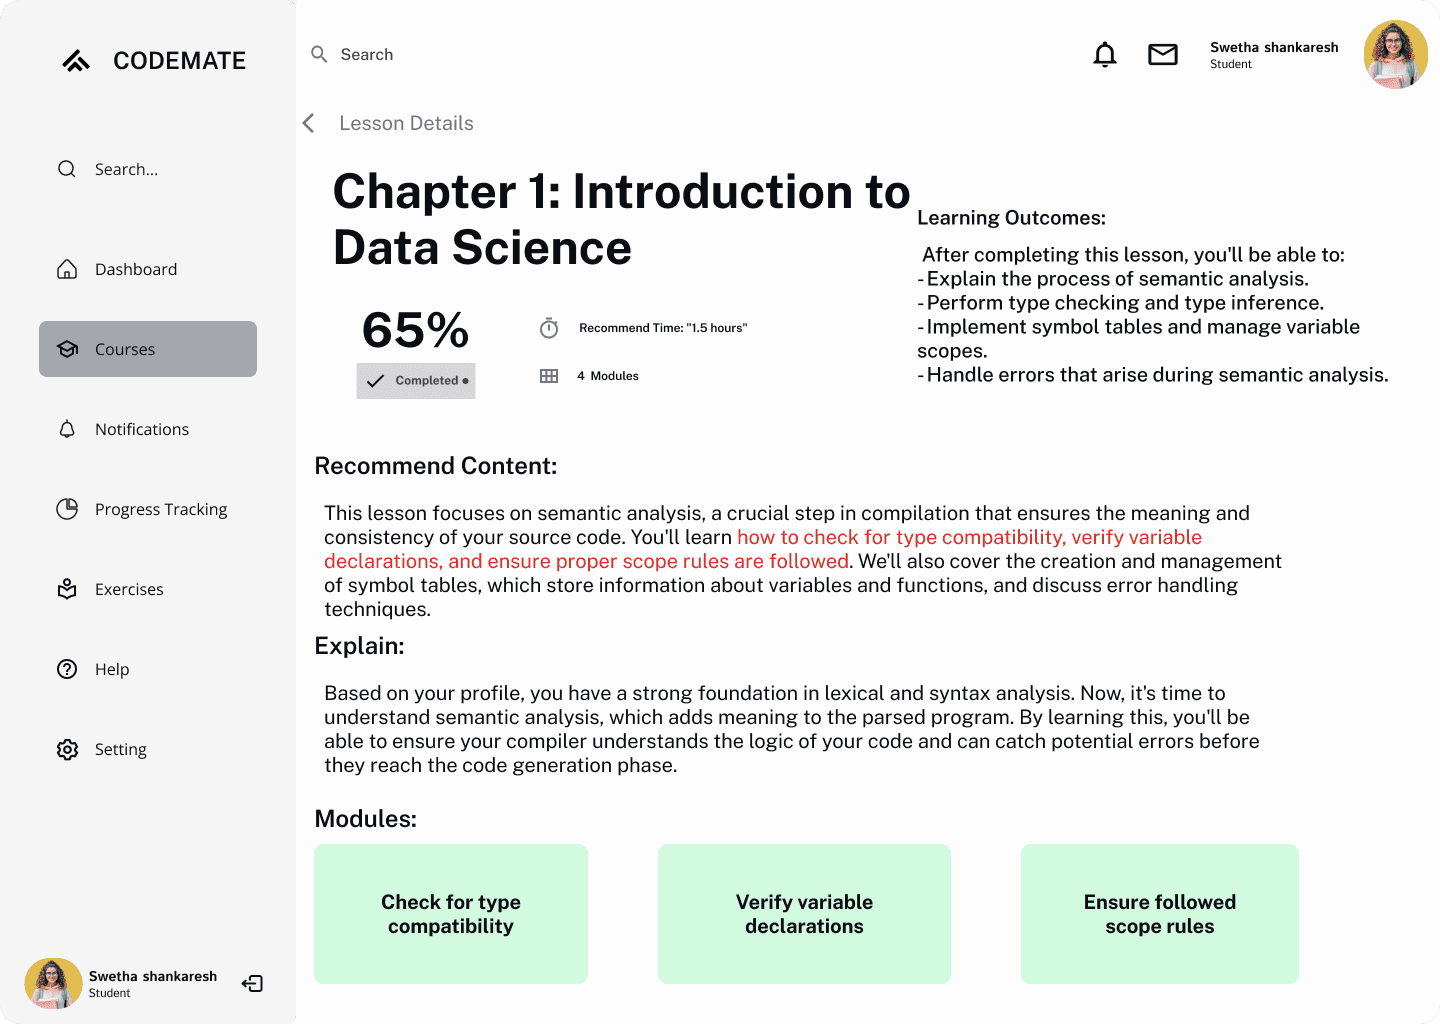
\includegraphics[scale=0.3]{Images/figmaDesign/Detailed Lesson Page.png}
    \caption{Chi tiết Lesson}
    \label{fig:enter-label}
\end{figure}
Lesson đề xuất sẽ cung cấp đầy đủ thông tin về \textbf{\textit{Learning Objectives, Recommend Content, Lời giải thích cho sự đề xuất và các modules cần học}}
\subsubsection{Choices of Learning Styles}
\begin{figure}[H]
    \centering
    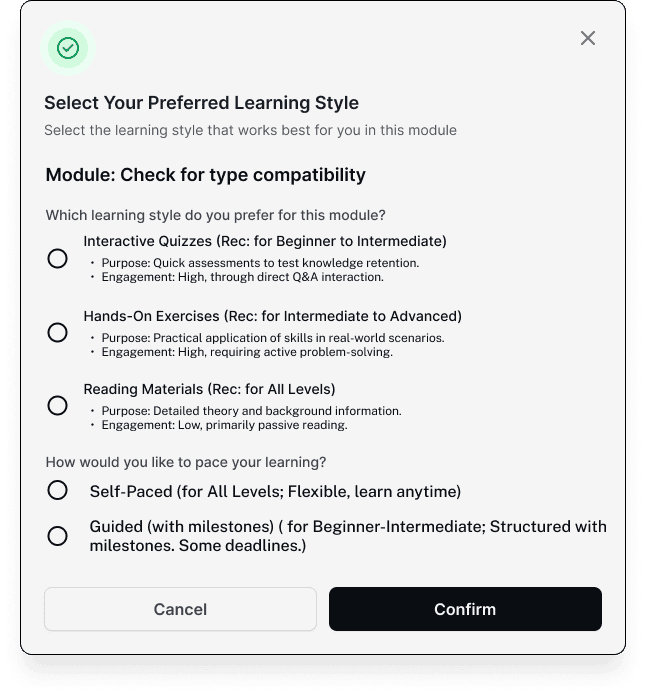
\includegraphics[scale=0.3]{Images/figmaDesign/Get Learning Style Modal.png}
    \caption{Modal cho phép sinh viên lựa chọn kiểu học phù hợp}
    \label{fig:enter-label}
\end{figure}
Sinh viên cung cấp thông tin về cách học mong muốn và tốc độ phù hợp với bản thân ở Modal này để quyết định cách học cho từng module
\begin{figure}[H]
    \centering
    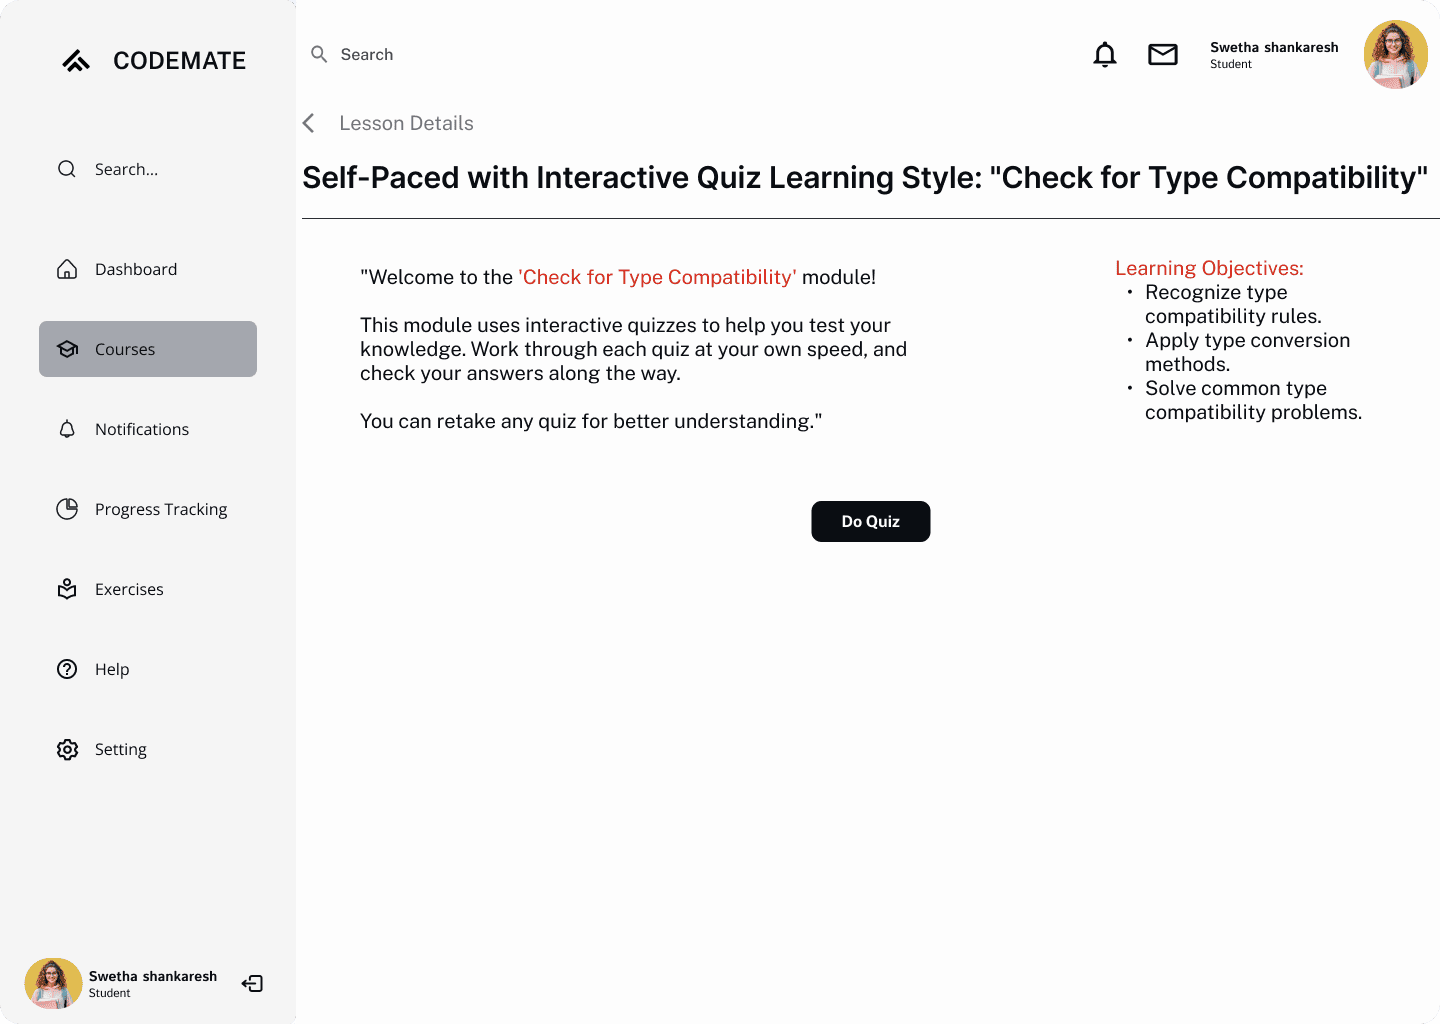
\includegraphics[scale=0.3]{Images/figmaDesign/Detailed Lesson Page - Self Pace Quiz.png}
    \caption{Giao diện khi sinh viên chọn học theo cách học làm Quiz với tiến độ tự do}
    \label{fig:enter-label}
\end{figure}
\begin{figure}[H]
    \centering
    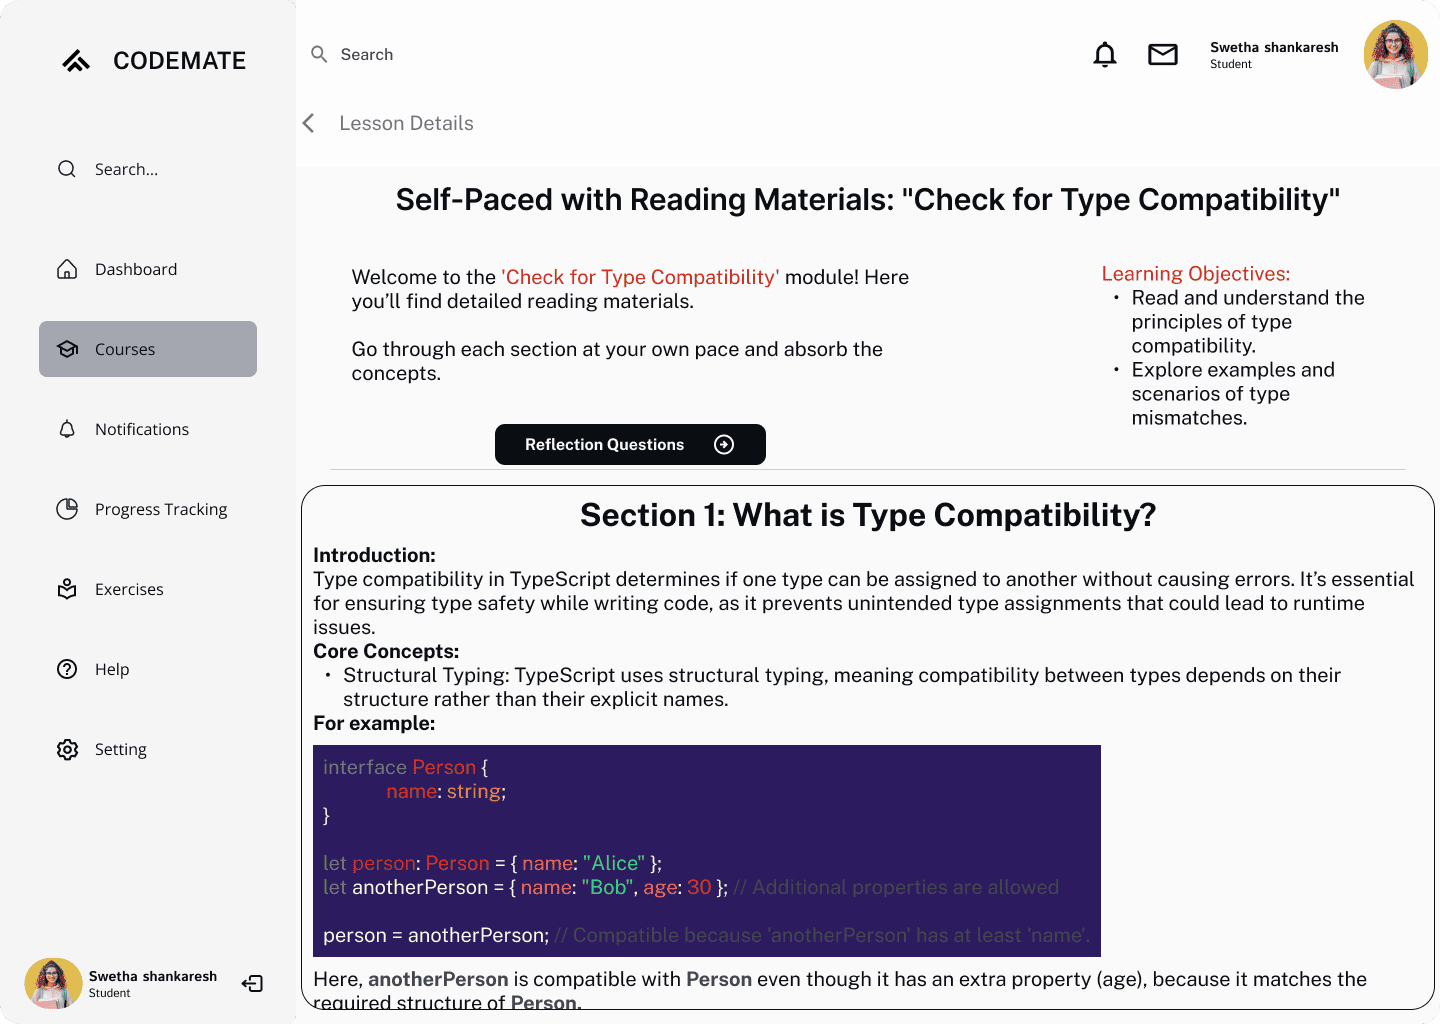
\includegraphics[scale=0.3]{Images/figmaDesign/Detailed Lesson Page - Self Pace Reading Material.png}
    \caption{Giao diện khi sinh viên chọn học theo cách học đọc tài liệu với tiến độ tự do}
    \label{fig:enter-label}
\end{figure}
\begin{figure}[H]
    \centering
    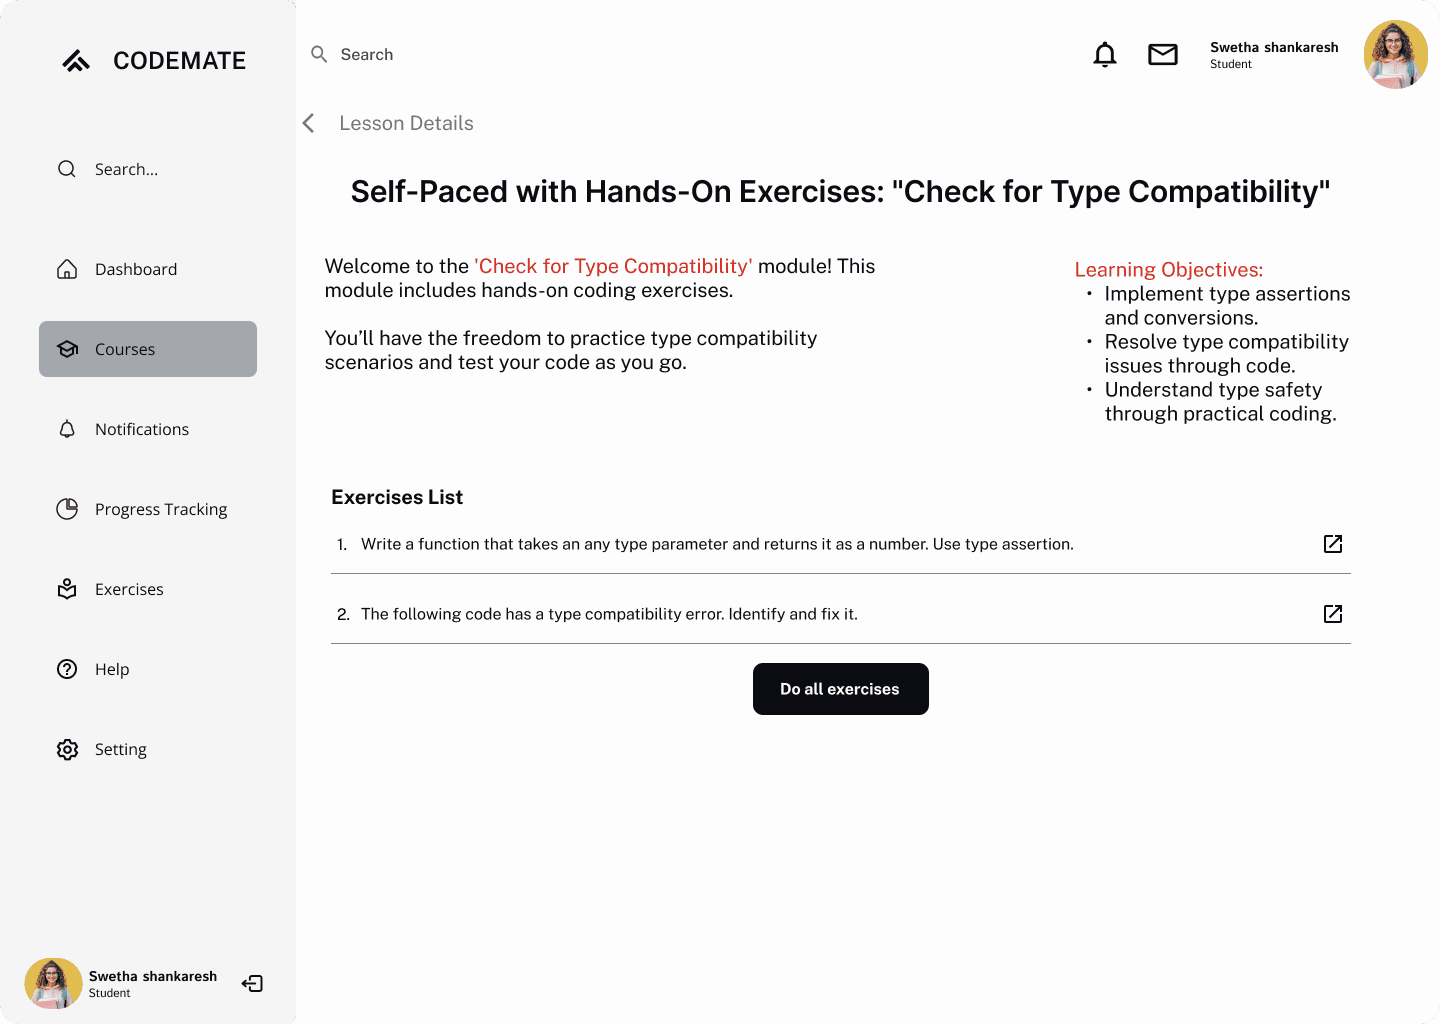
\includegraphics[scale=0.3]{Images/figmaDesign/Detailed Lesson Page - Self Pace Hands On Exercise.png}
    \caption{Giao diện khi sinh viên chọn học theo cách học làm bài tập Coding với tiến độ tự do}
    \label{fig:enter-label}
\end{figure}
\subsection{User Profile}
\subsubsection{Profile Information}
\begin{figure}[H]
    \centering
    \begin{subfigure}[b]{0.45\linewidth}
        \centering
        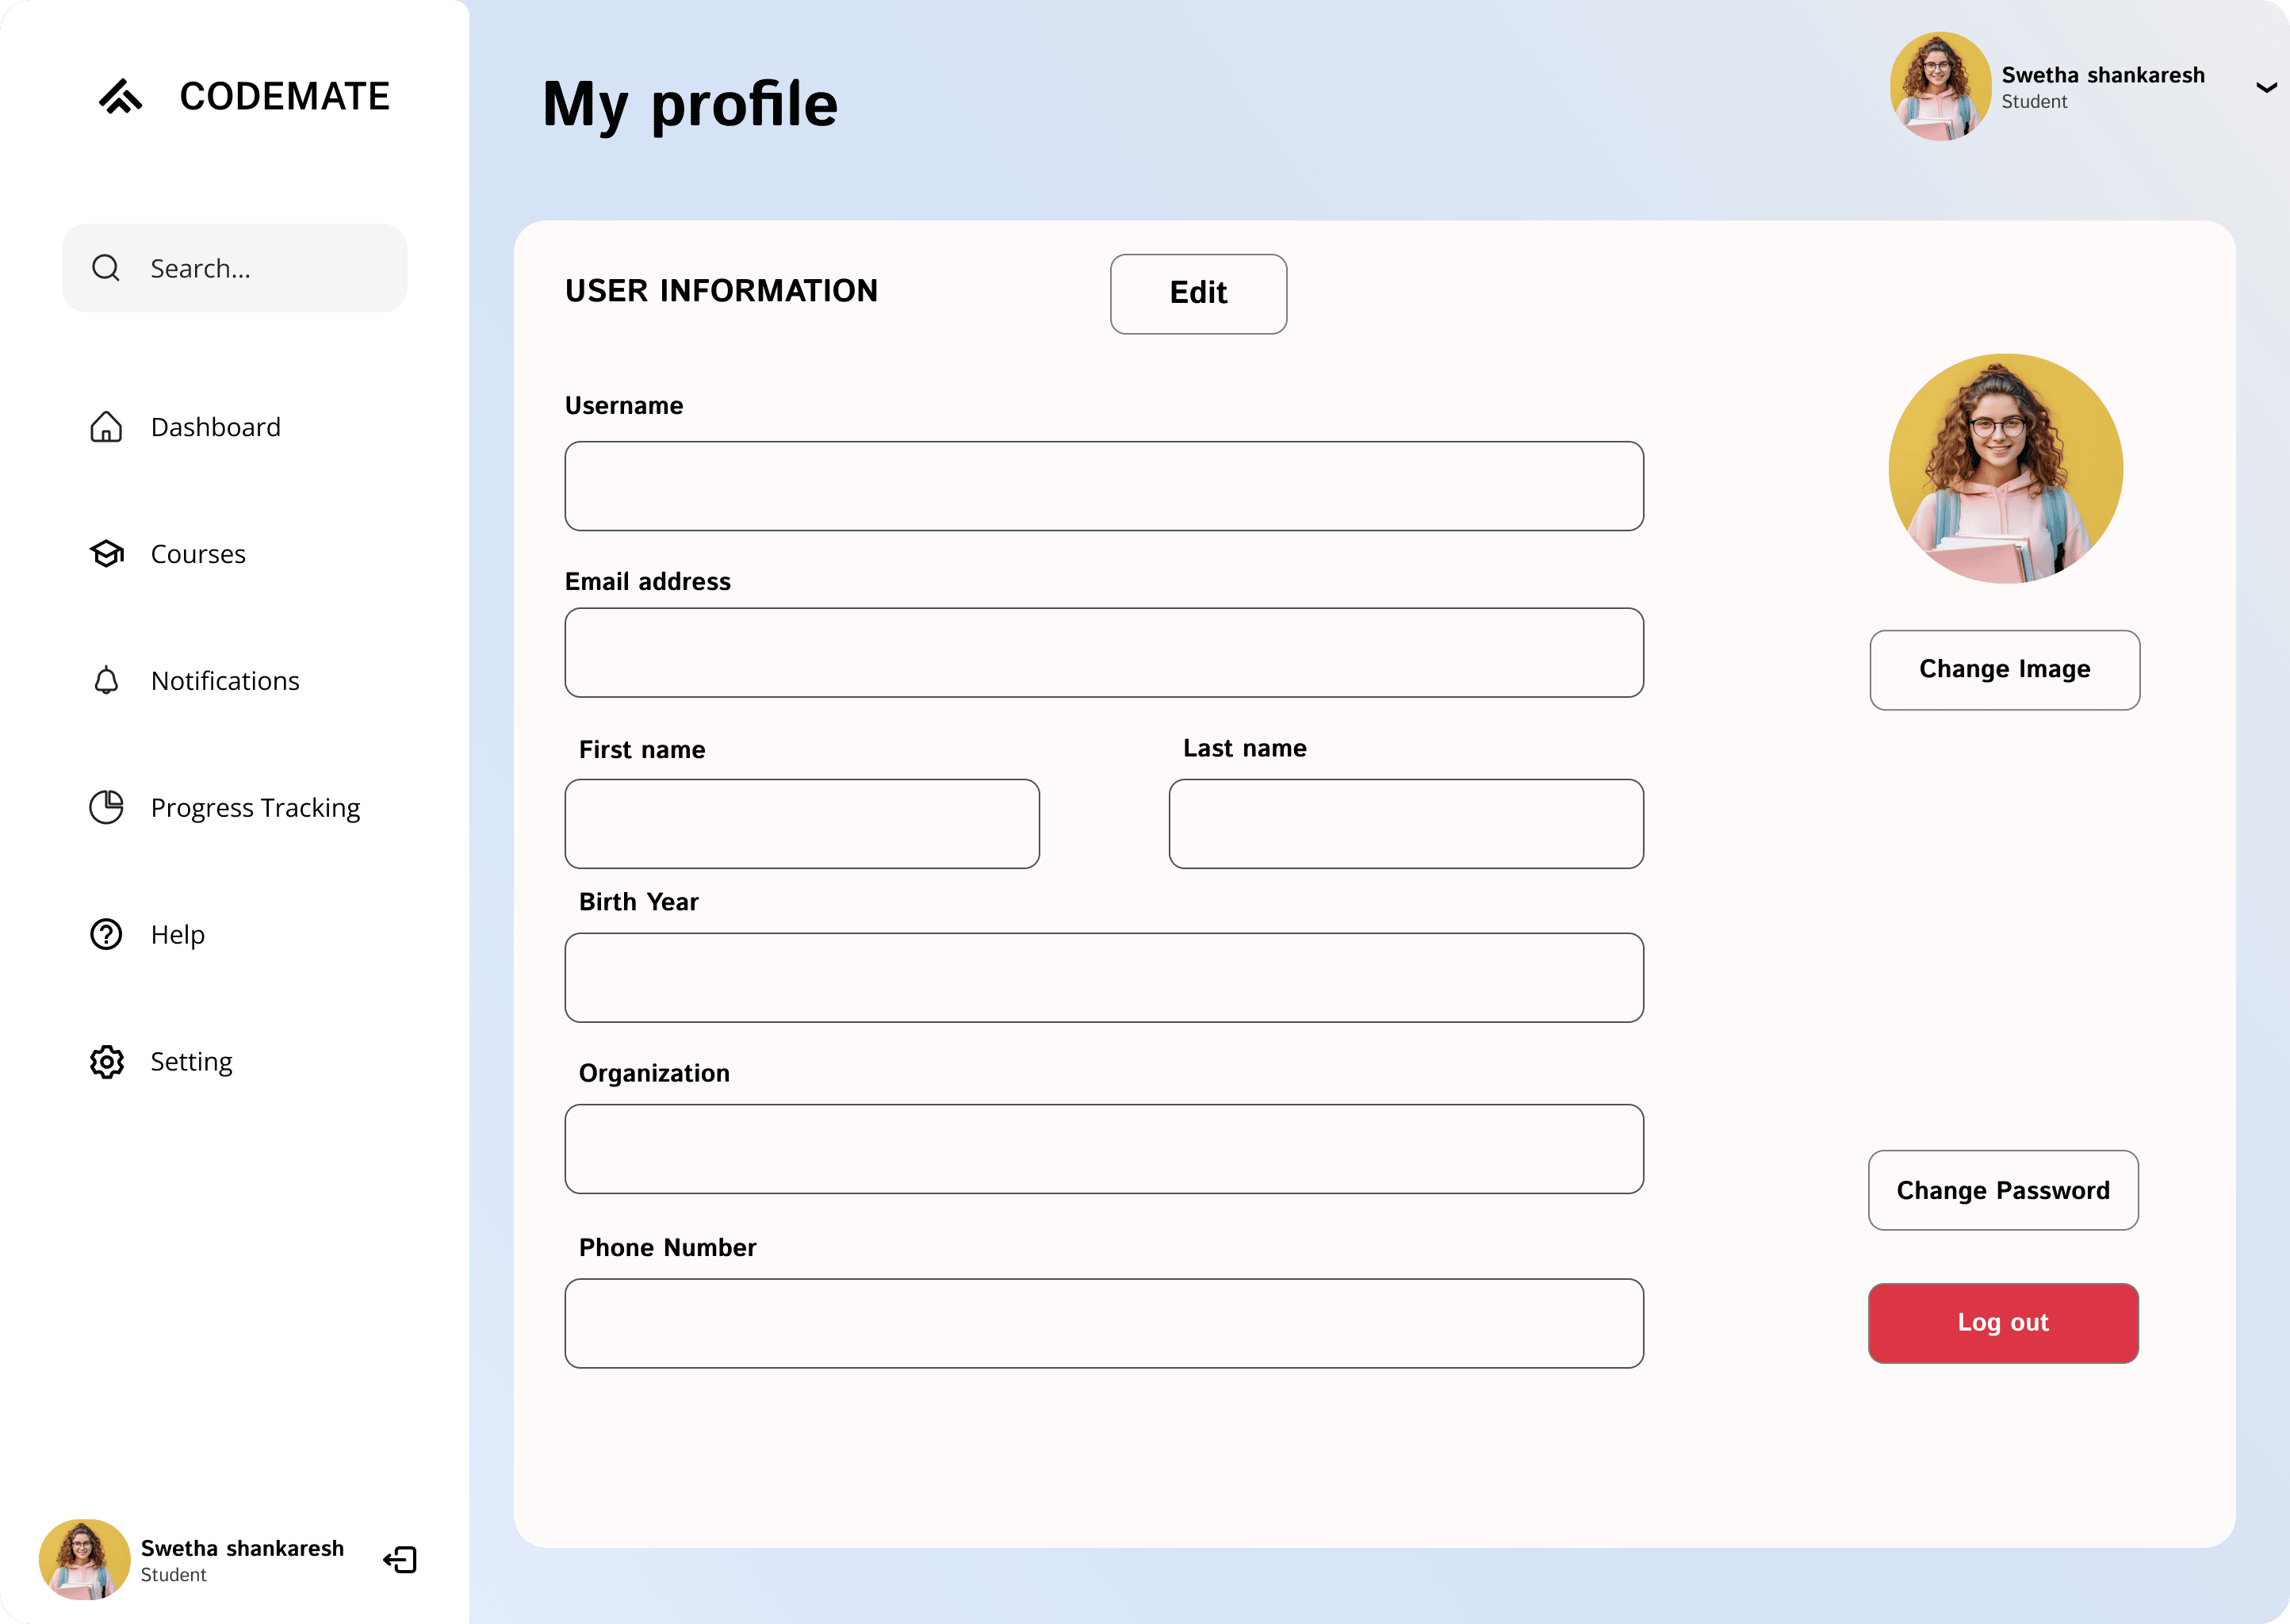
\includegraphics[width=\linewidth]{Images/Anh/UI_profile.png}
        \caption{Trang thông tin tài khoản}
        \label{fig:enter-label1}
    \end{subfigure}
    \hfill
    \begin{subfigure}[b]{0.45\linewidth}
        \centering
        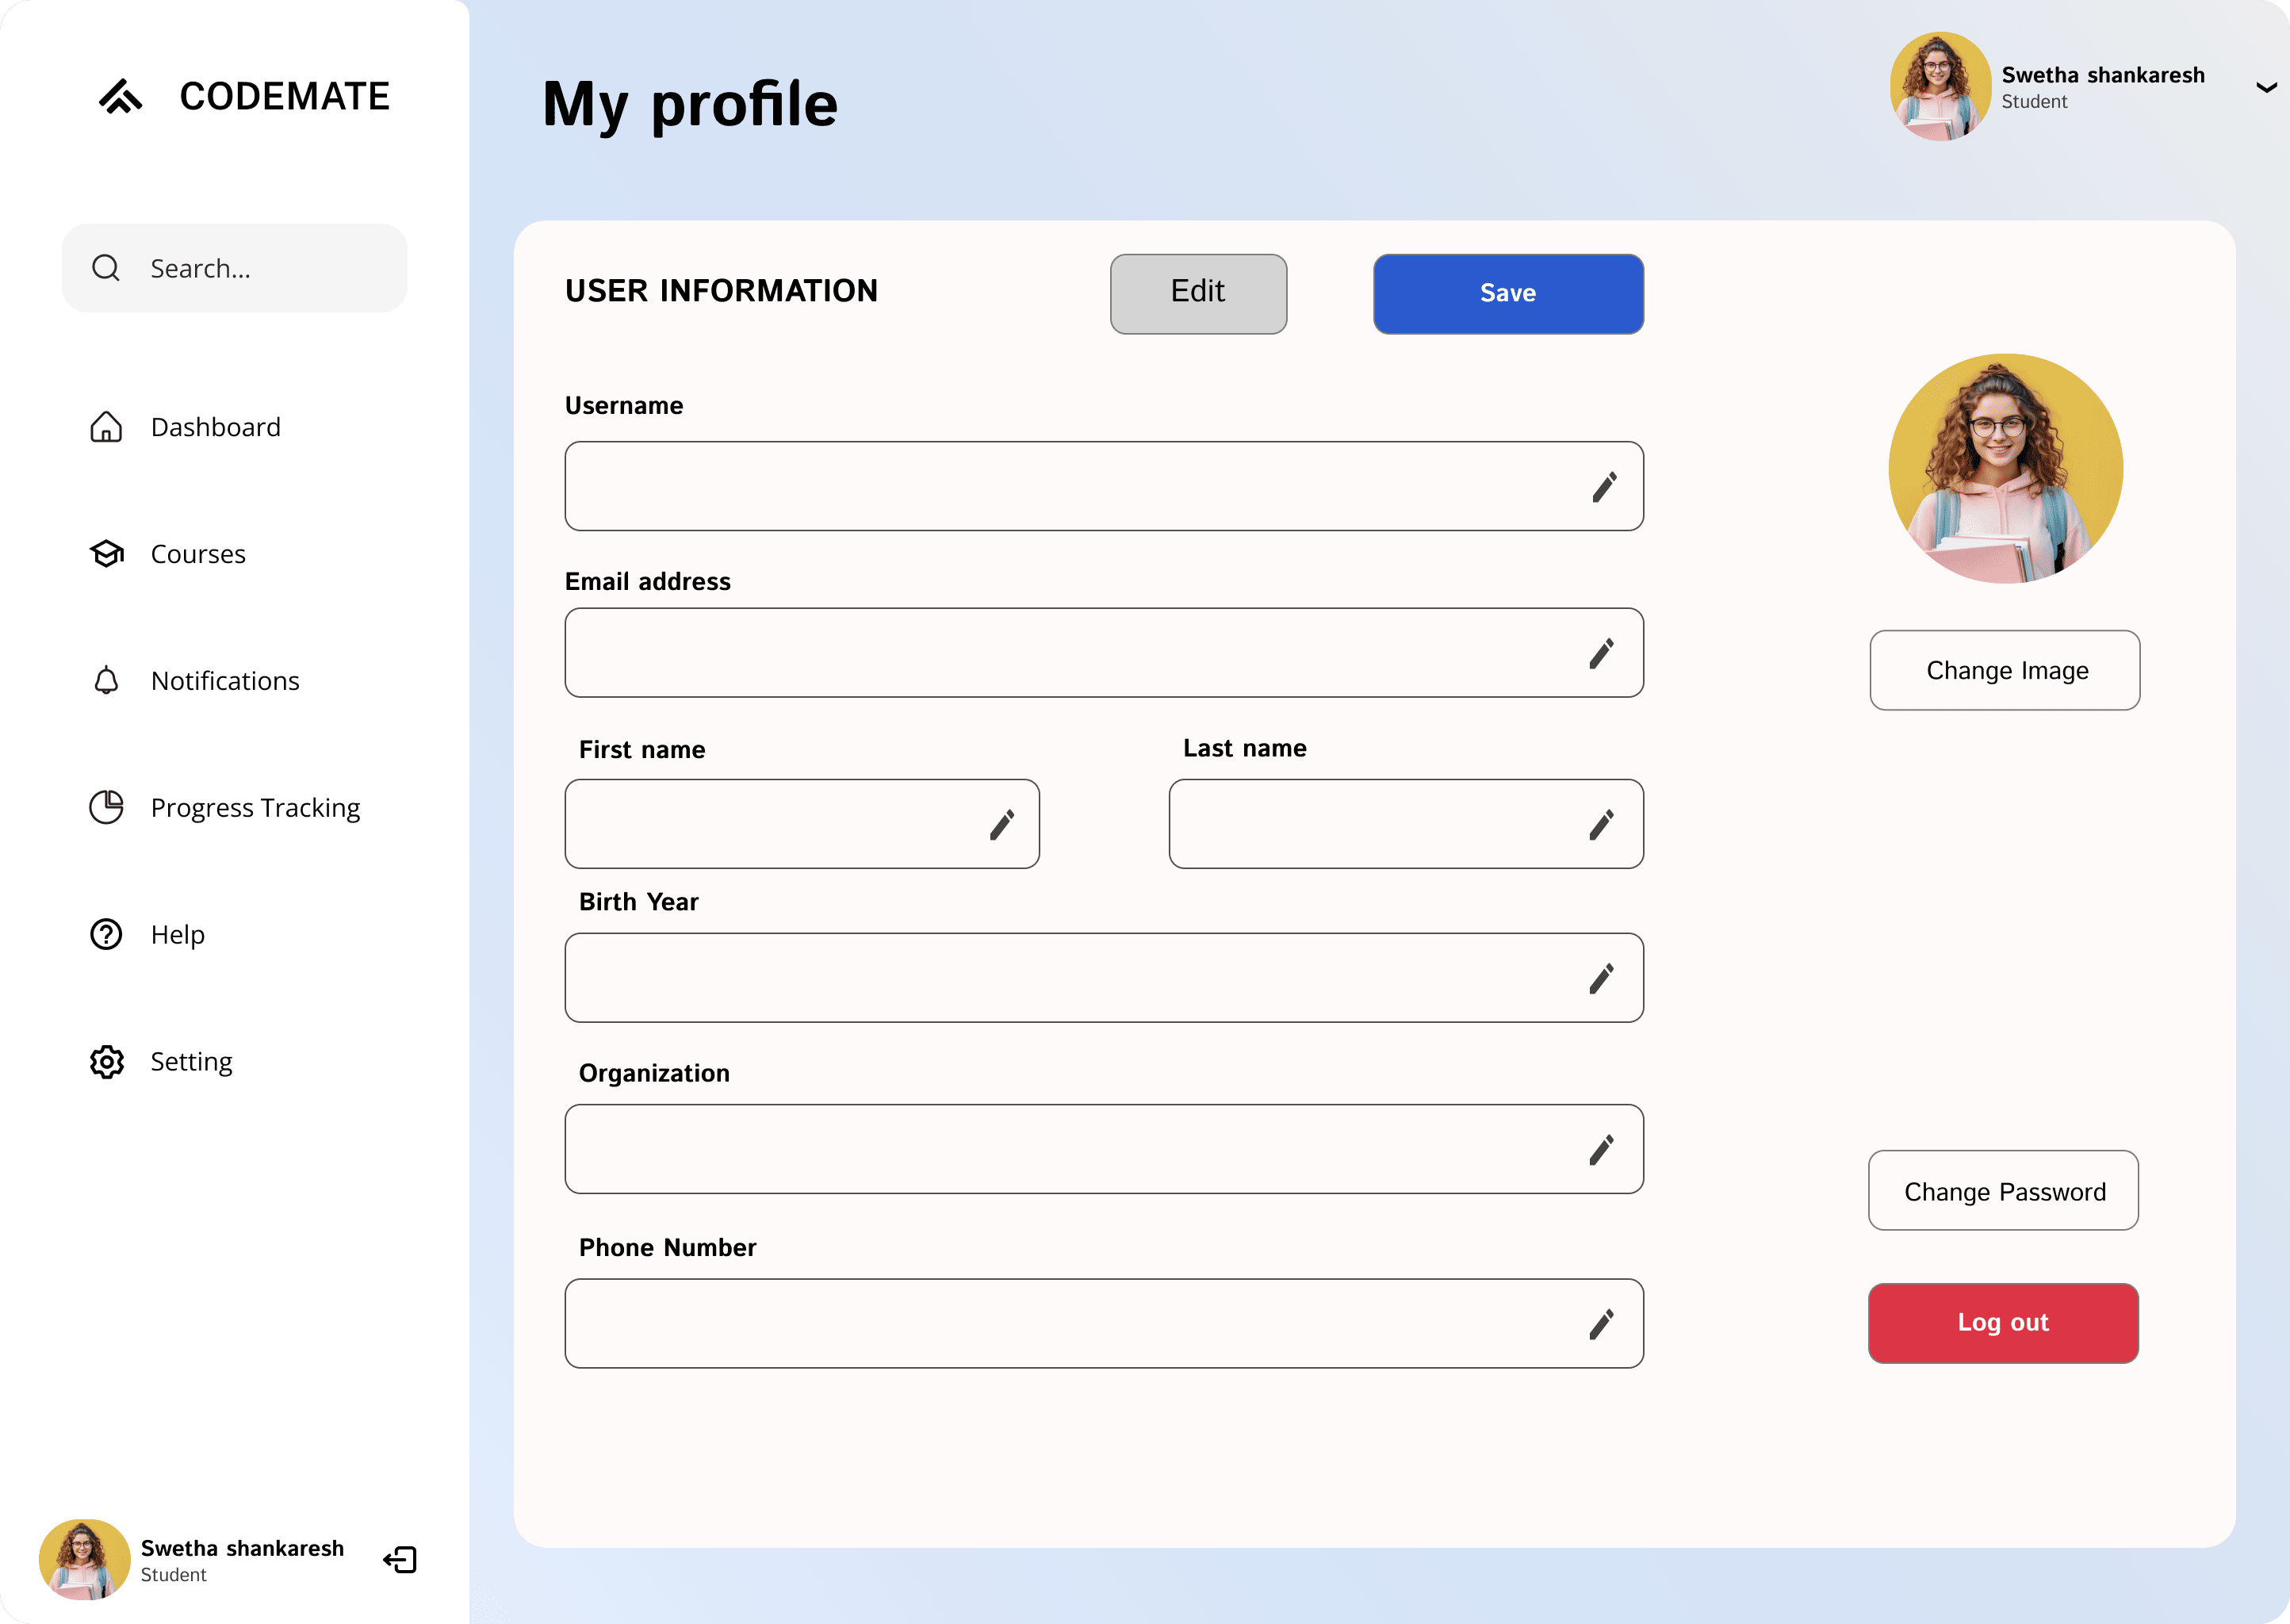
\includegraphics[width=\linewidth]{Images/Anh/UI_edit_profile.png}
        \caption{Chỉnh sửa thông tin tài khoản}
        \label{fig:enter-label2}
    \end{subfigure}
    \label{fig:enter-label}
\end{figure}
Trang "Thông tin tài khoản" cung cấp các trường thông tin cá nhân của người dùng bao gồm: Tên người dùng (Username), Địa chỉ email (Email address), Tên (First name), Họ (Last name), Năm sinh (Birth Year), Trường (Organization), và Số điện thoại (Phone Number). Người dùng có thể thay đổi hình ảnh đại diện bằng cách nhấp vào nút Change Image và cập nhật mật khẩu thông qua nút Change Password. Tất cả thông tin có thể được chỉnh sửa bằng cách nhấn vào nút Edit.
\subsubsection{Change Password, Avatar}
\begin{figure}[H]
    \centering
    \begin{subfigure}[b]{0.45\linewidth}
        \centering
        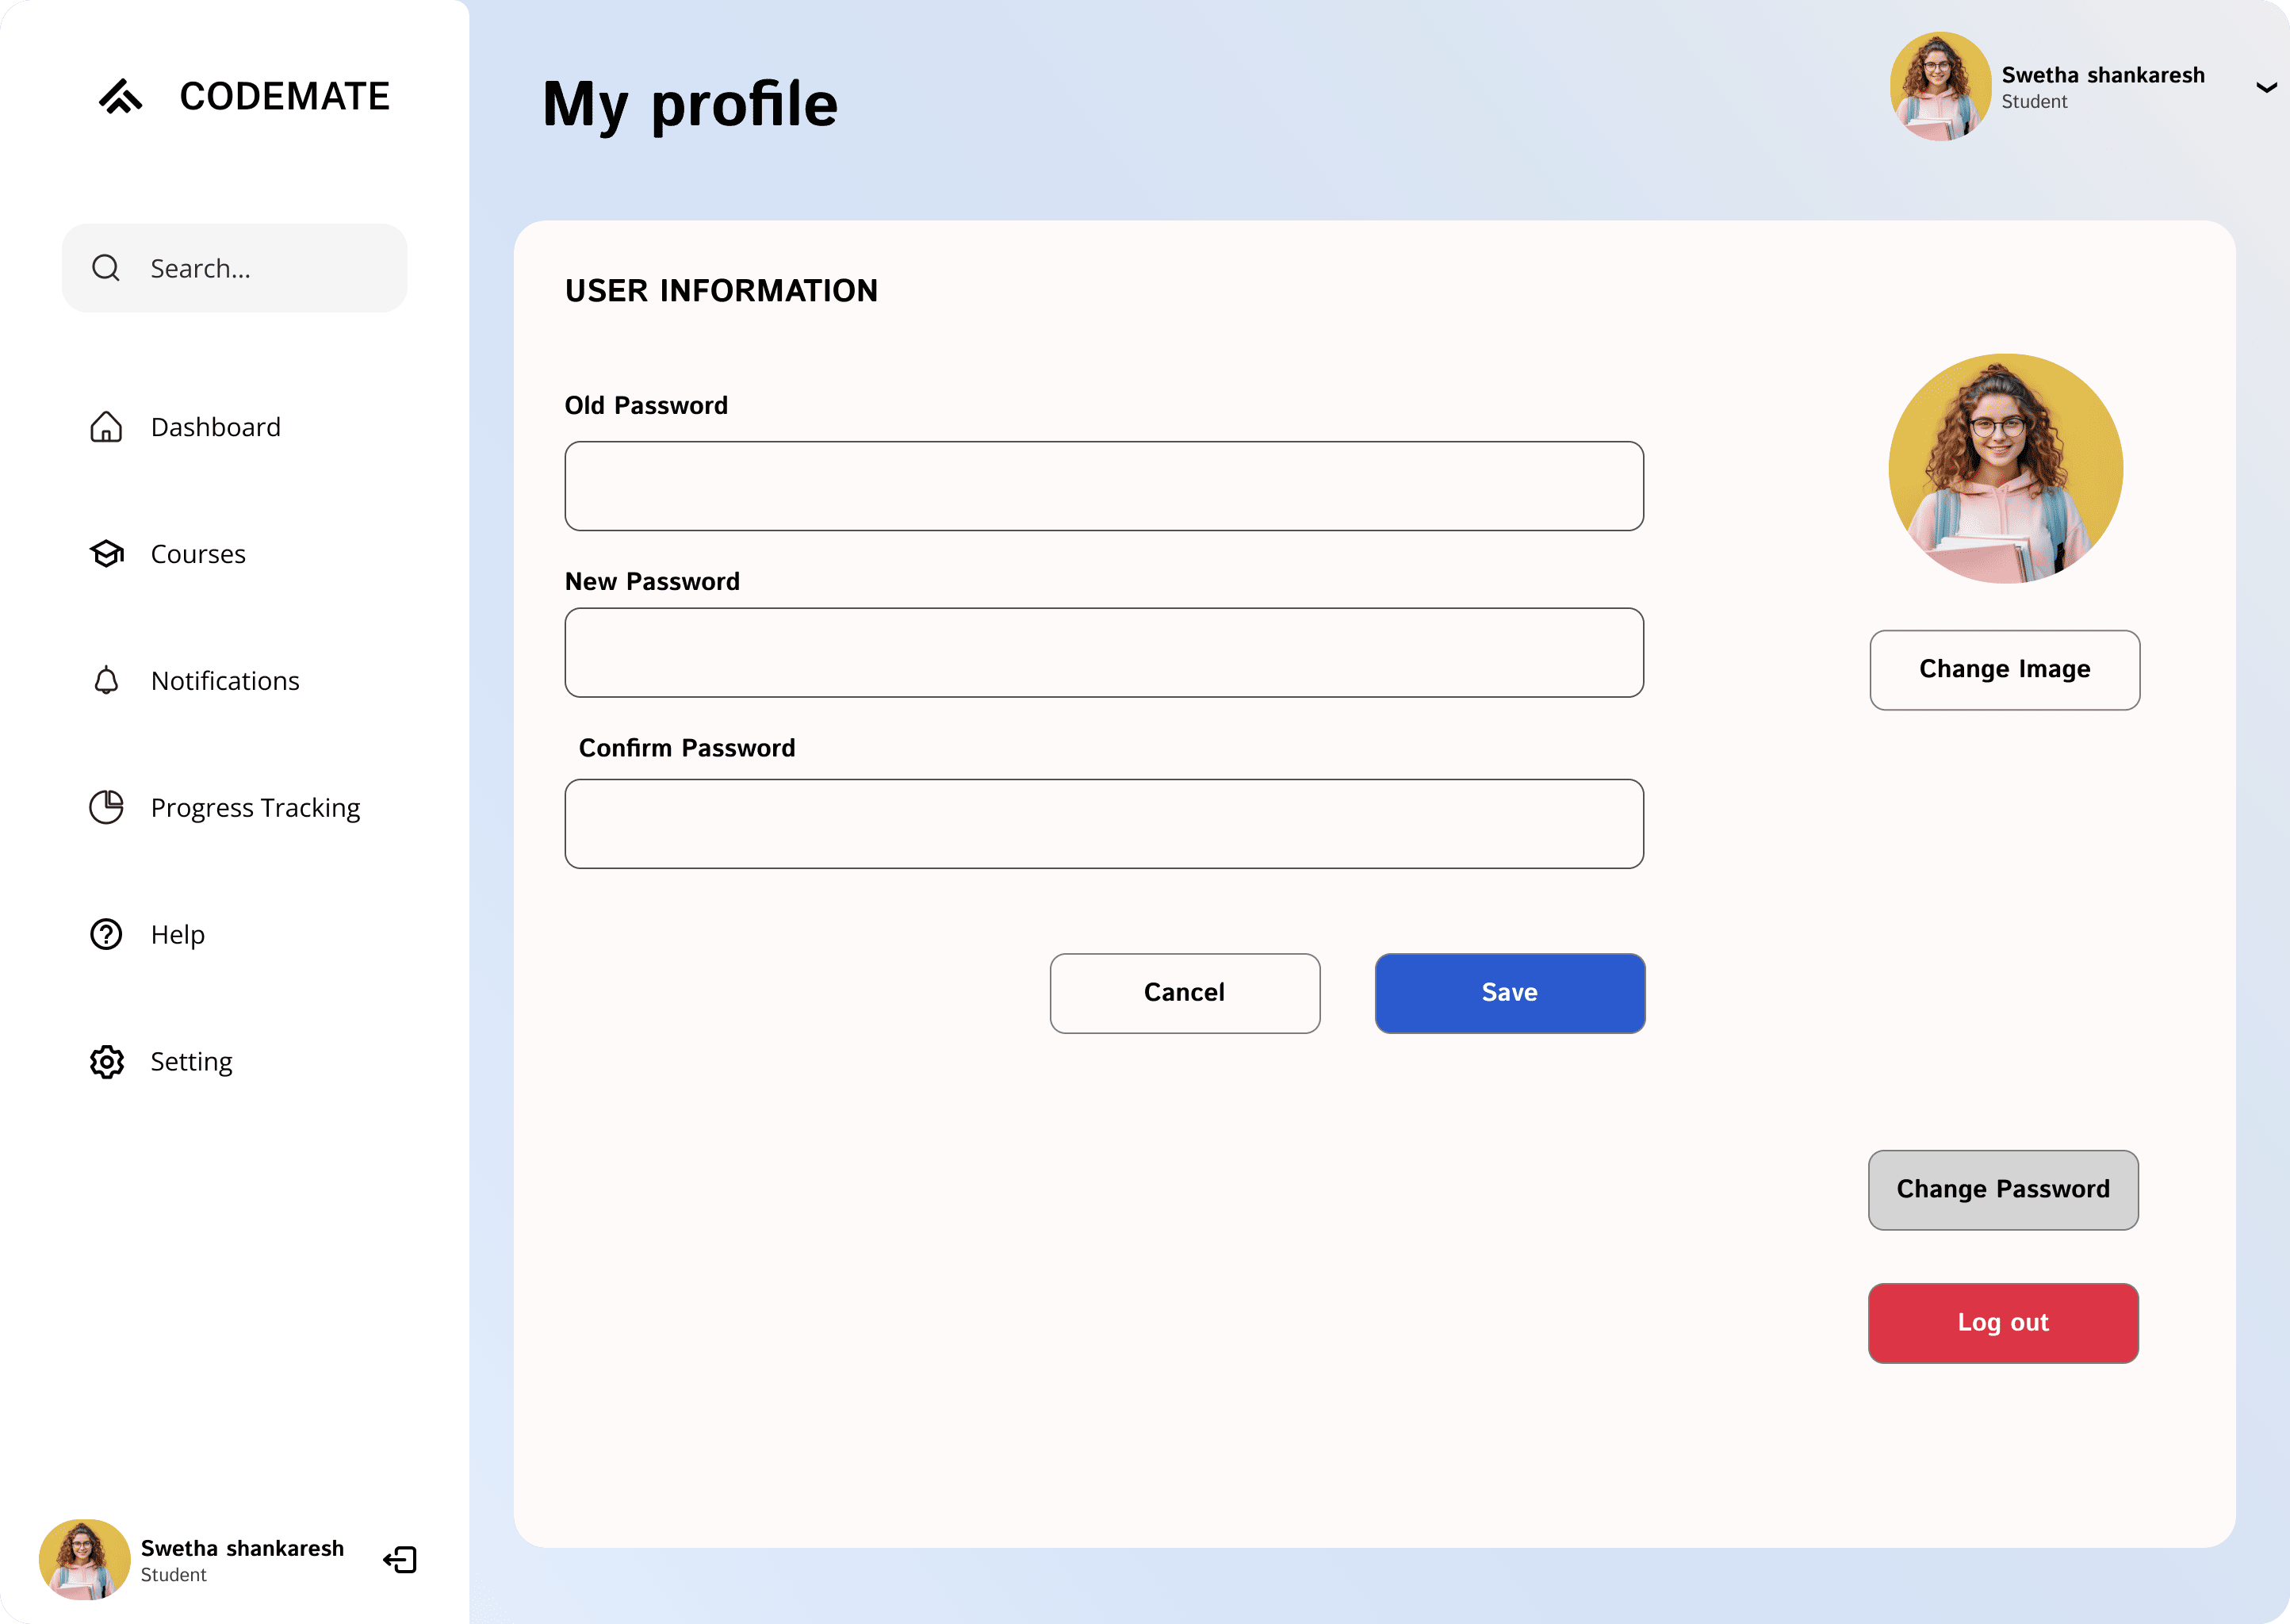
\includegraphics[width=\linewidth]{Images/Anh/UI_change_pass.png}
        \caption{Thay đổi mật khẩu}
        \label{fig:enter-label1}
    \end{subfigure}
    \hfill
    \begin{subfigure}[b]{0.45\linewidth}
        \centering
        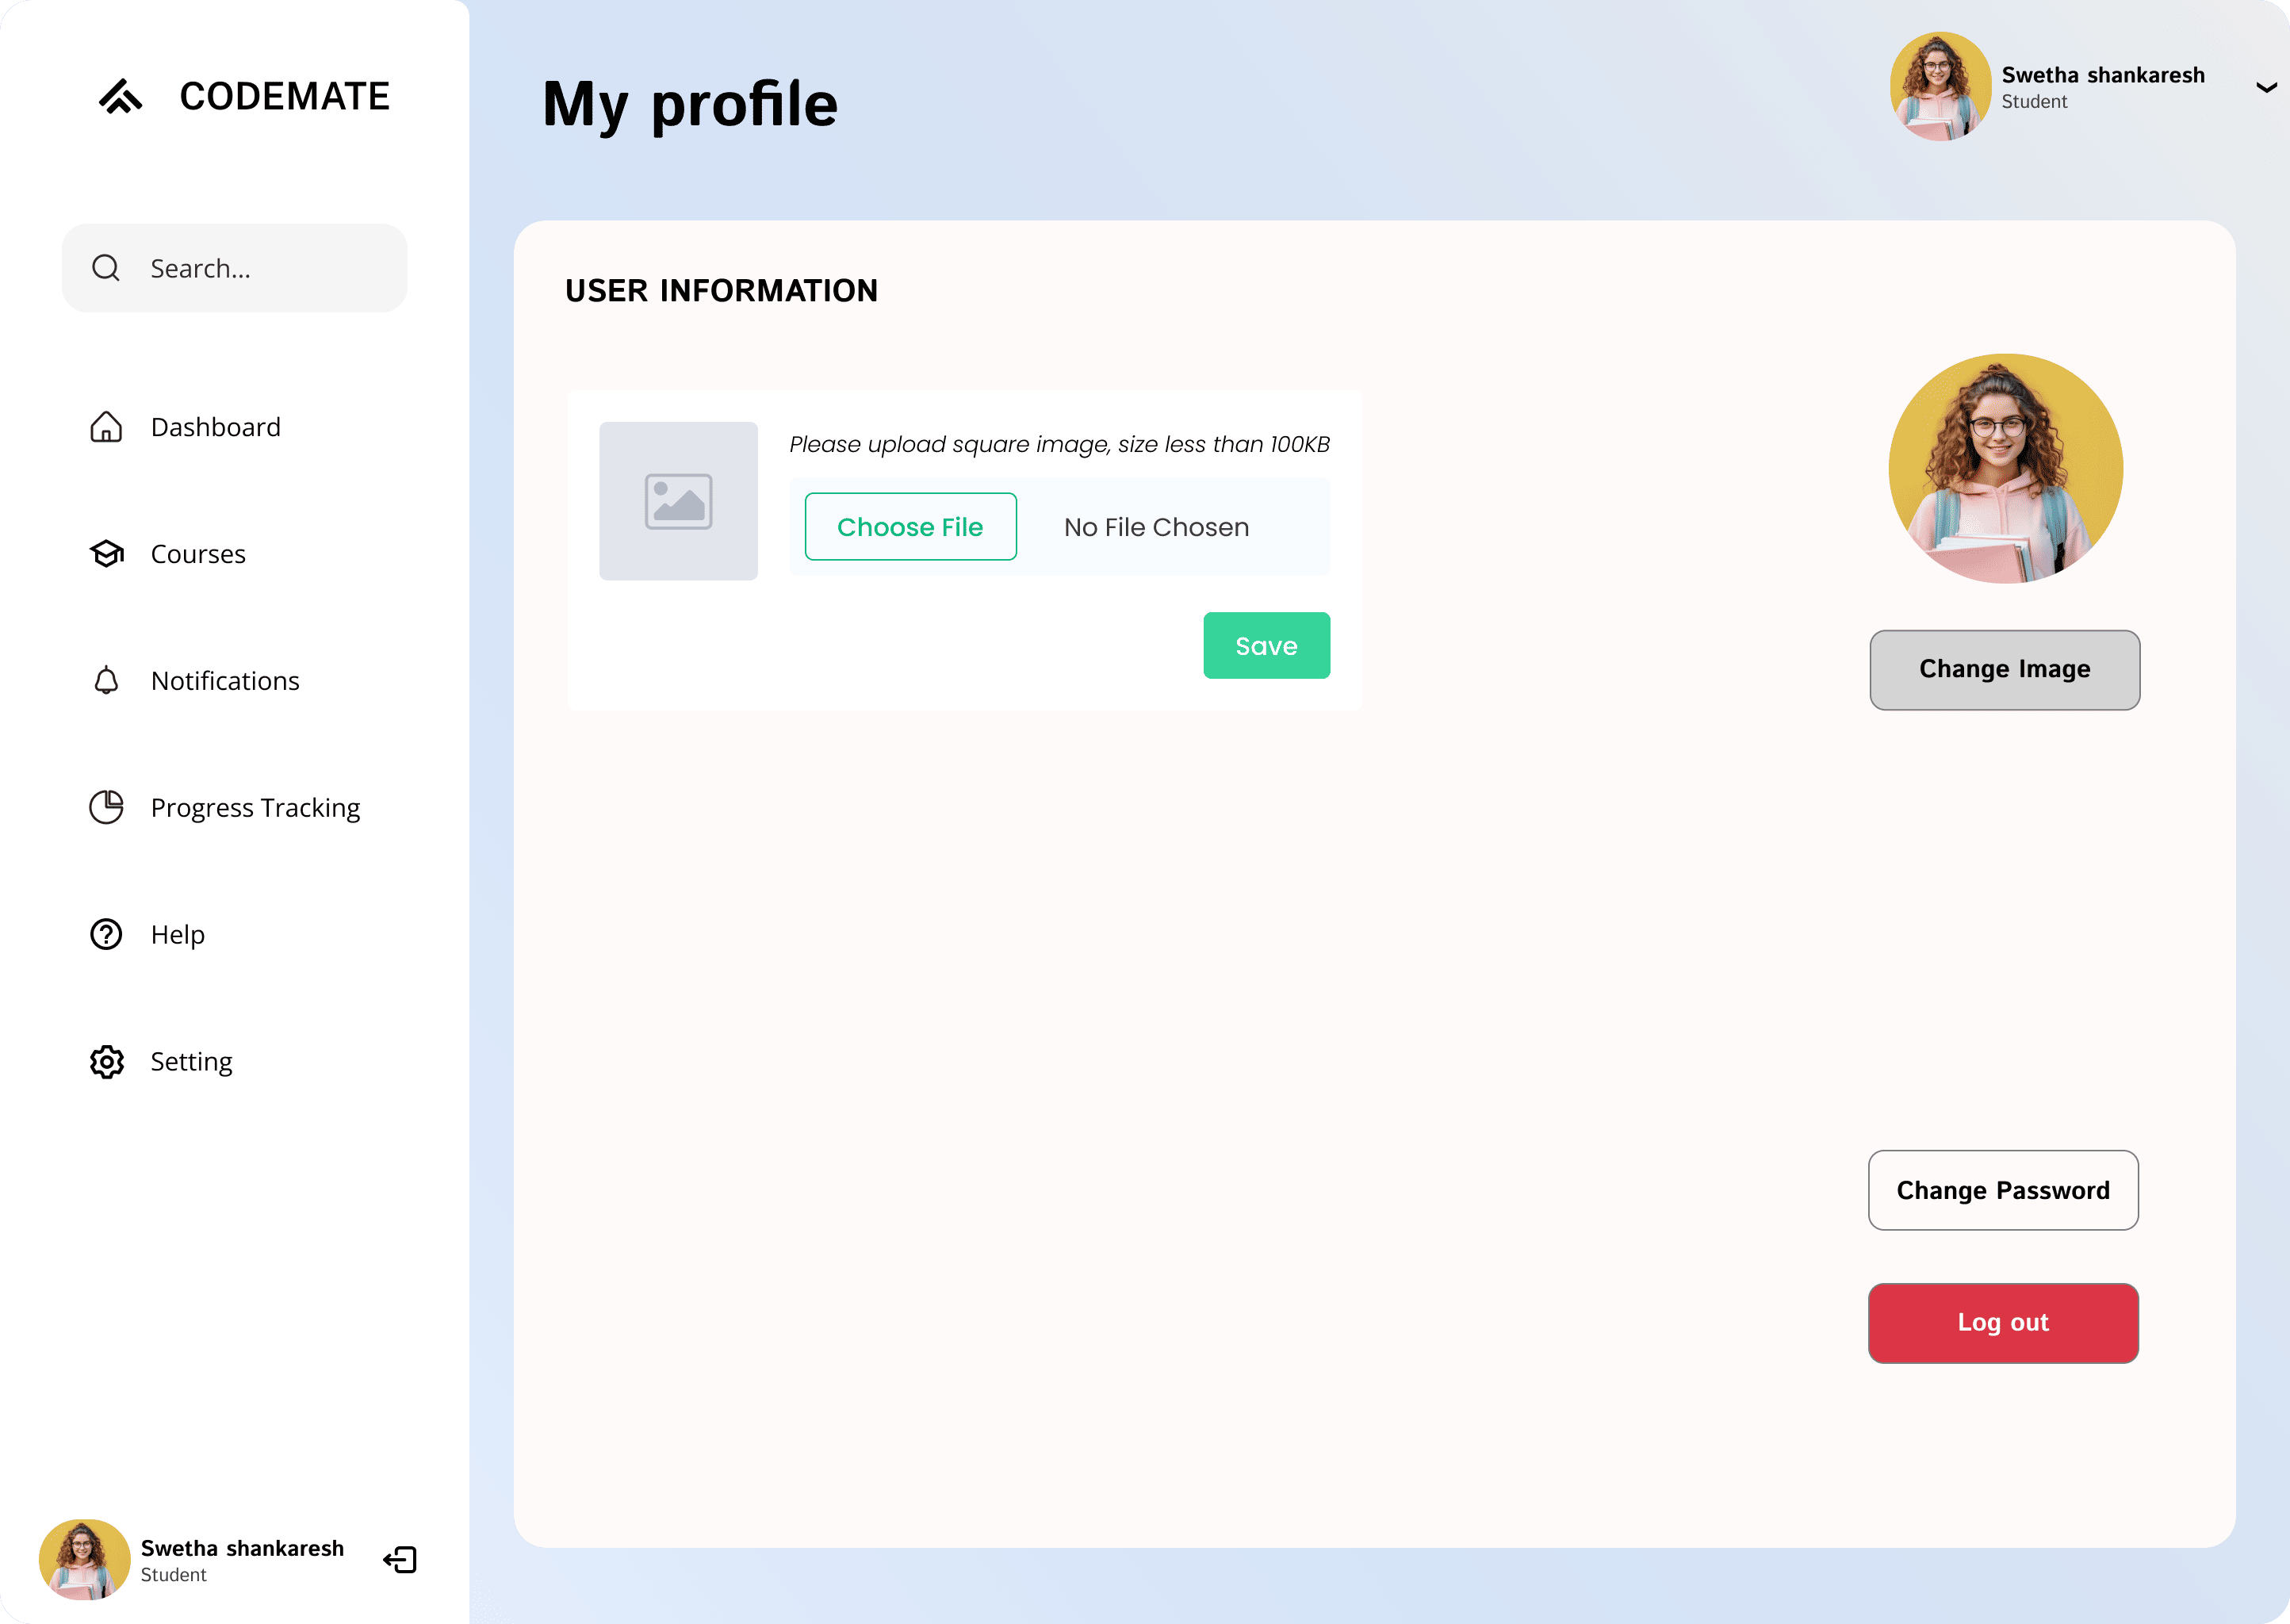
\includegraphics[width=\linewidth]{Images/Anh/UI_change_avatar.png}
        \caption{Thay đổi avatar}
        \label{fig:enter-label2}
    \end{subfigure}
    \label{fig:enter-label}
\end{figure}
Trang "Đổi mật khẩu" cho phép người dùng thay đổi mật khẩu bằng cách nhập mật khẩu hiện tại, mật khẩu mới, và xác nhận lại mật khẩu mới. Sau khi điền đầy đủ thông tin, người dùng nhấn nút "Đổi mật khẩu" để hoàn tất. Nếu có lỗi hoặc thành công, hệ thống sẽ hiển thị thông báo tương ứng. Trang "Đổi ảnh đại diện" cho phép người dùng tải lên ảnh mới từ thiết bị của mình và nhấn "Lưu thay đổi" để cập nhật ảnh đại diện.
\subsection{Dashboard Screen}
\begin{figure}[H]
    \centering
    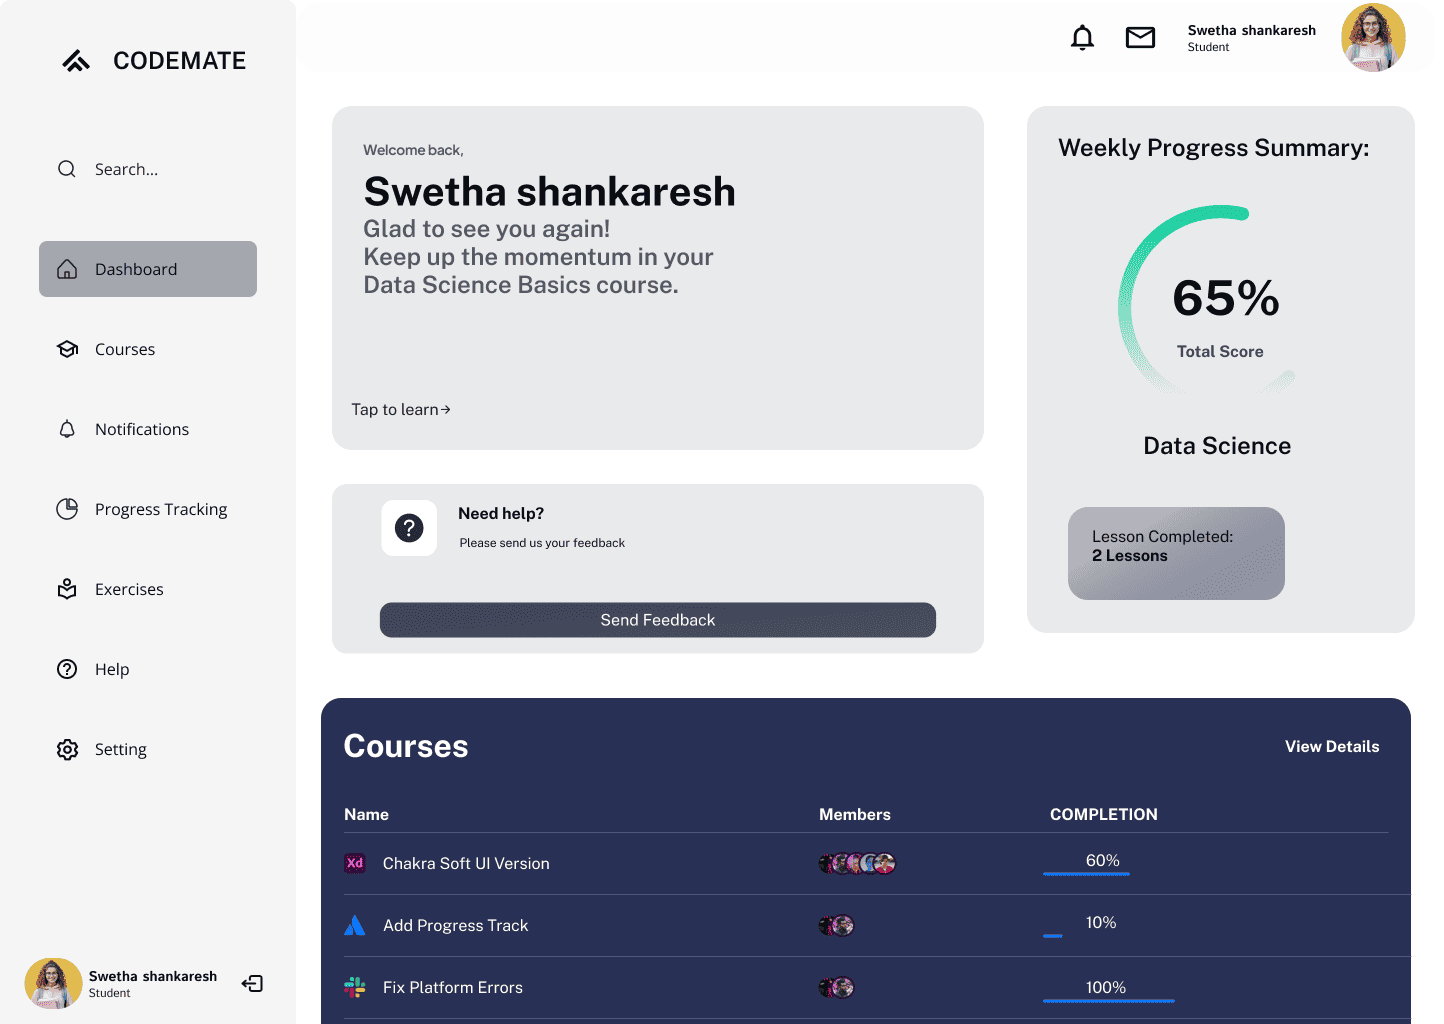
\includegraphics[width=1\linewidth]{Images/figmaDesign/Dashboard - Student.png}
    \caption{Dashboard - Student}
    \label{fig:enter-label}
\end{figure}
Trang Dashboard của sinh viên, mô tả tóm tắt về các khóa học mà sinh viên đã và đang tham gia và một số thông tin về khóa học vừa học ở lần truy cập gần nhất.
\subsection{Exercise Practice}
\subsubsection{Code Exercise}
\begin{figure}[H]
    \centering
    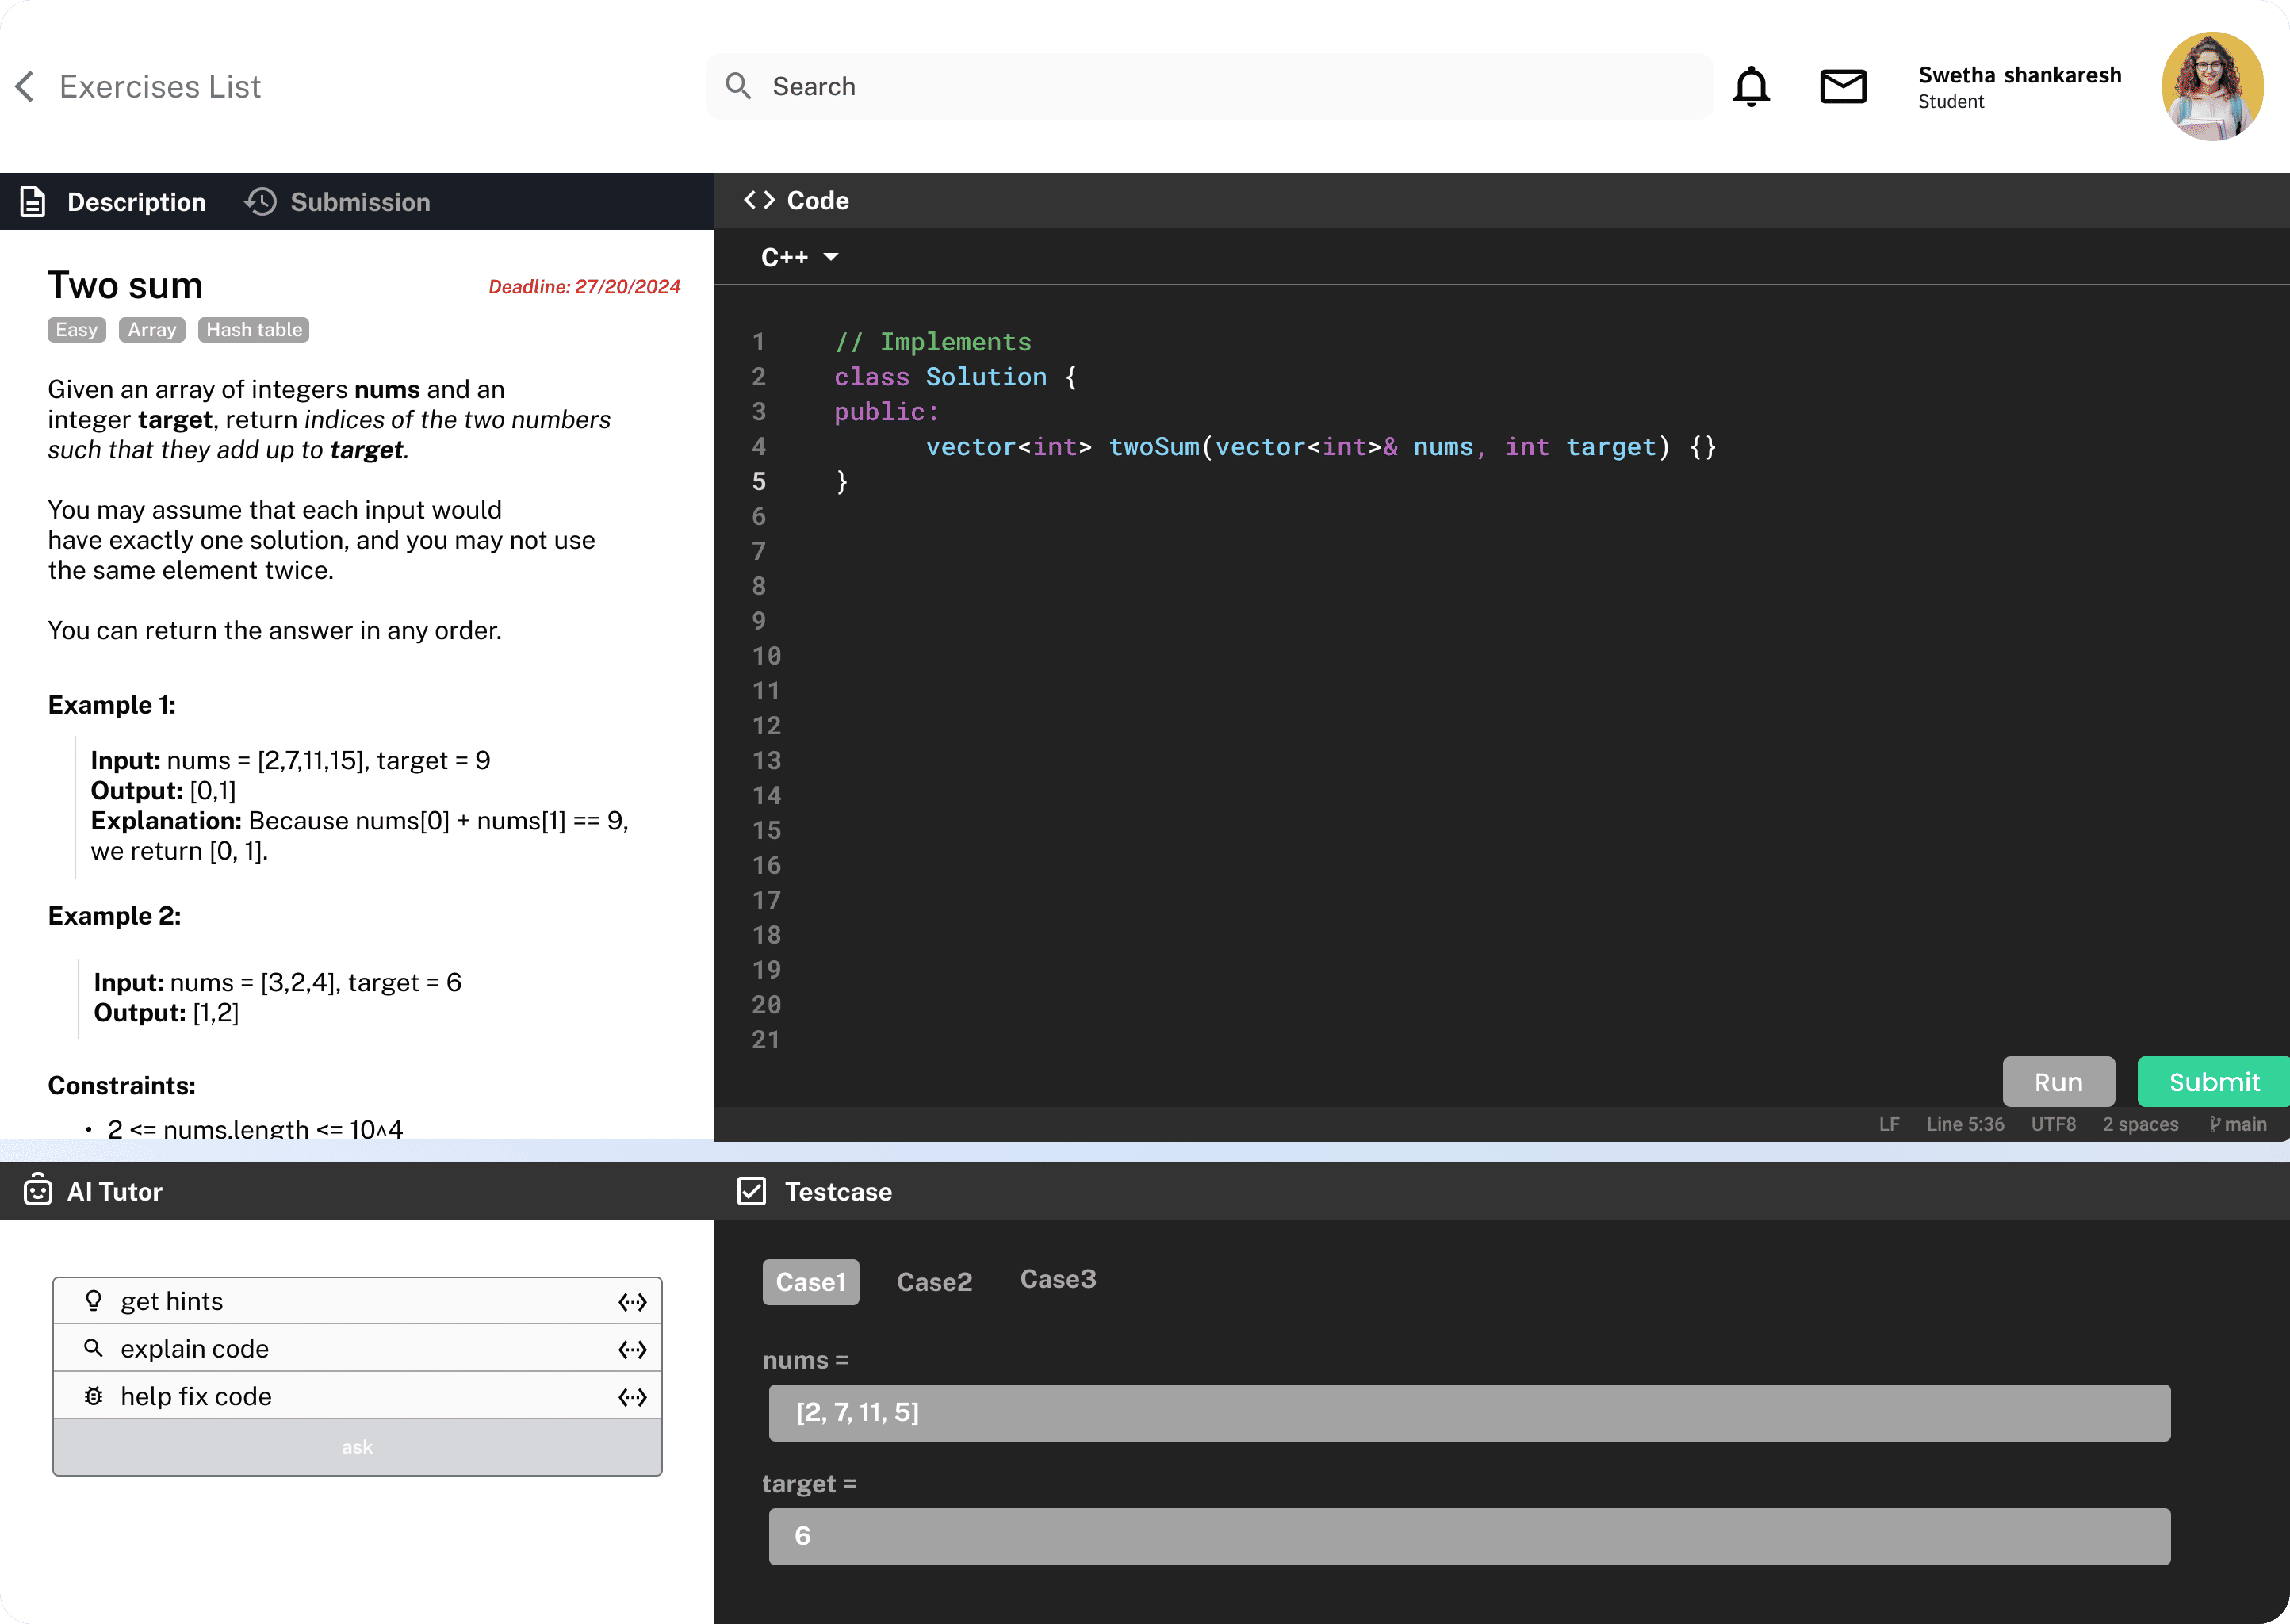
\includegraphics[width=0.7\linewidth]{Images/Anh/UI_practice_code.png}
    \caption{Giao diện thực hành code}
    \label{fig:enter-label}
\end{figure}
\begin{figure}[H]
    \centering
    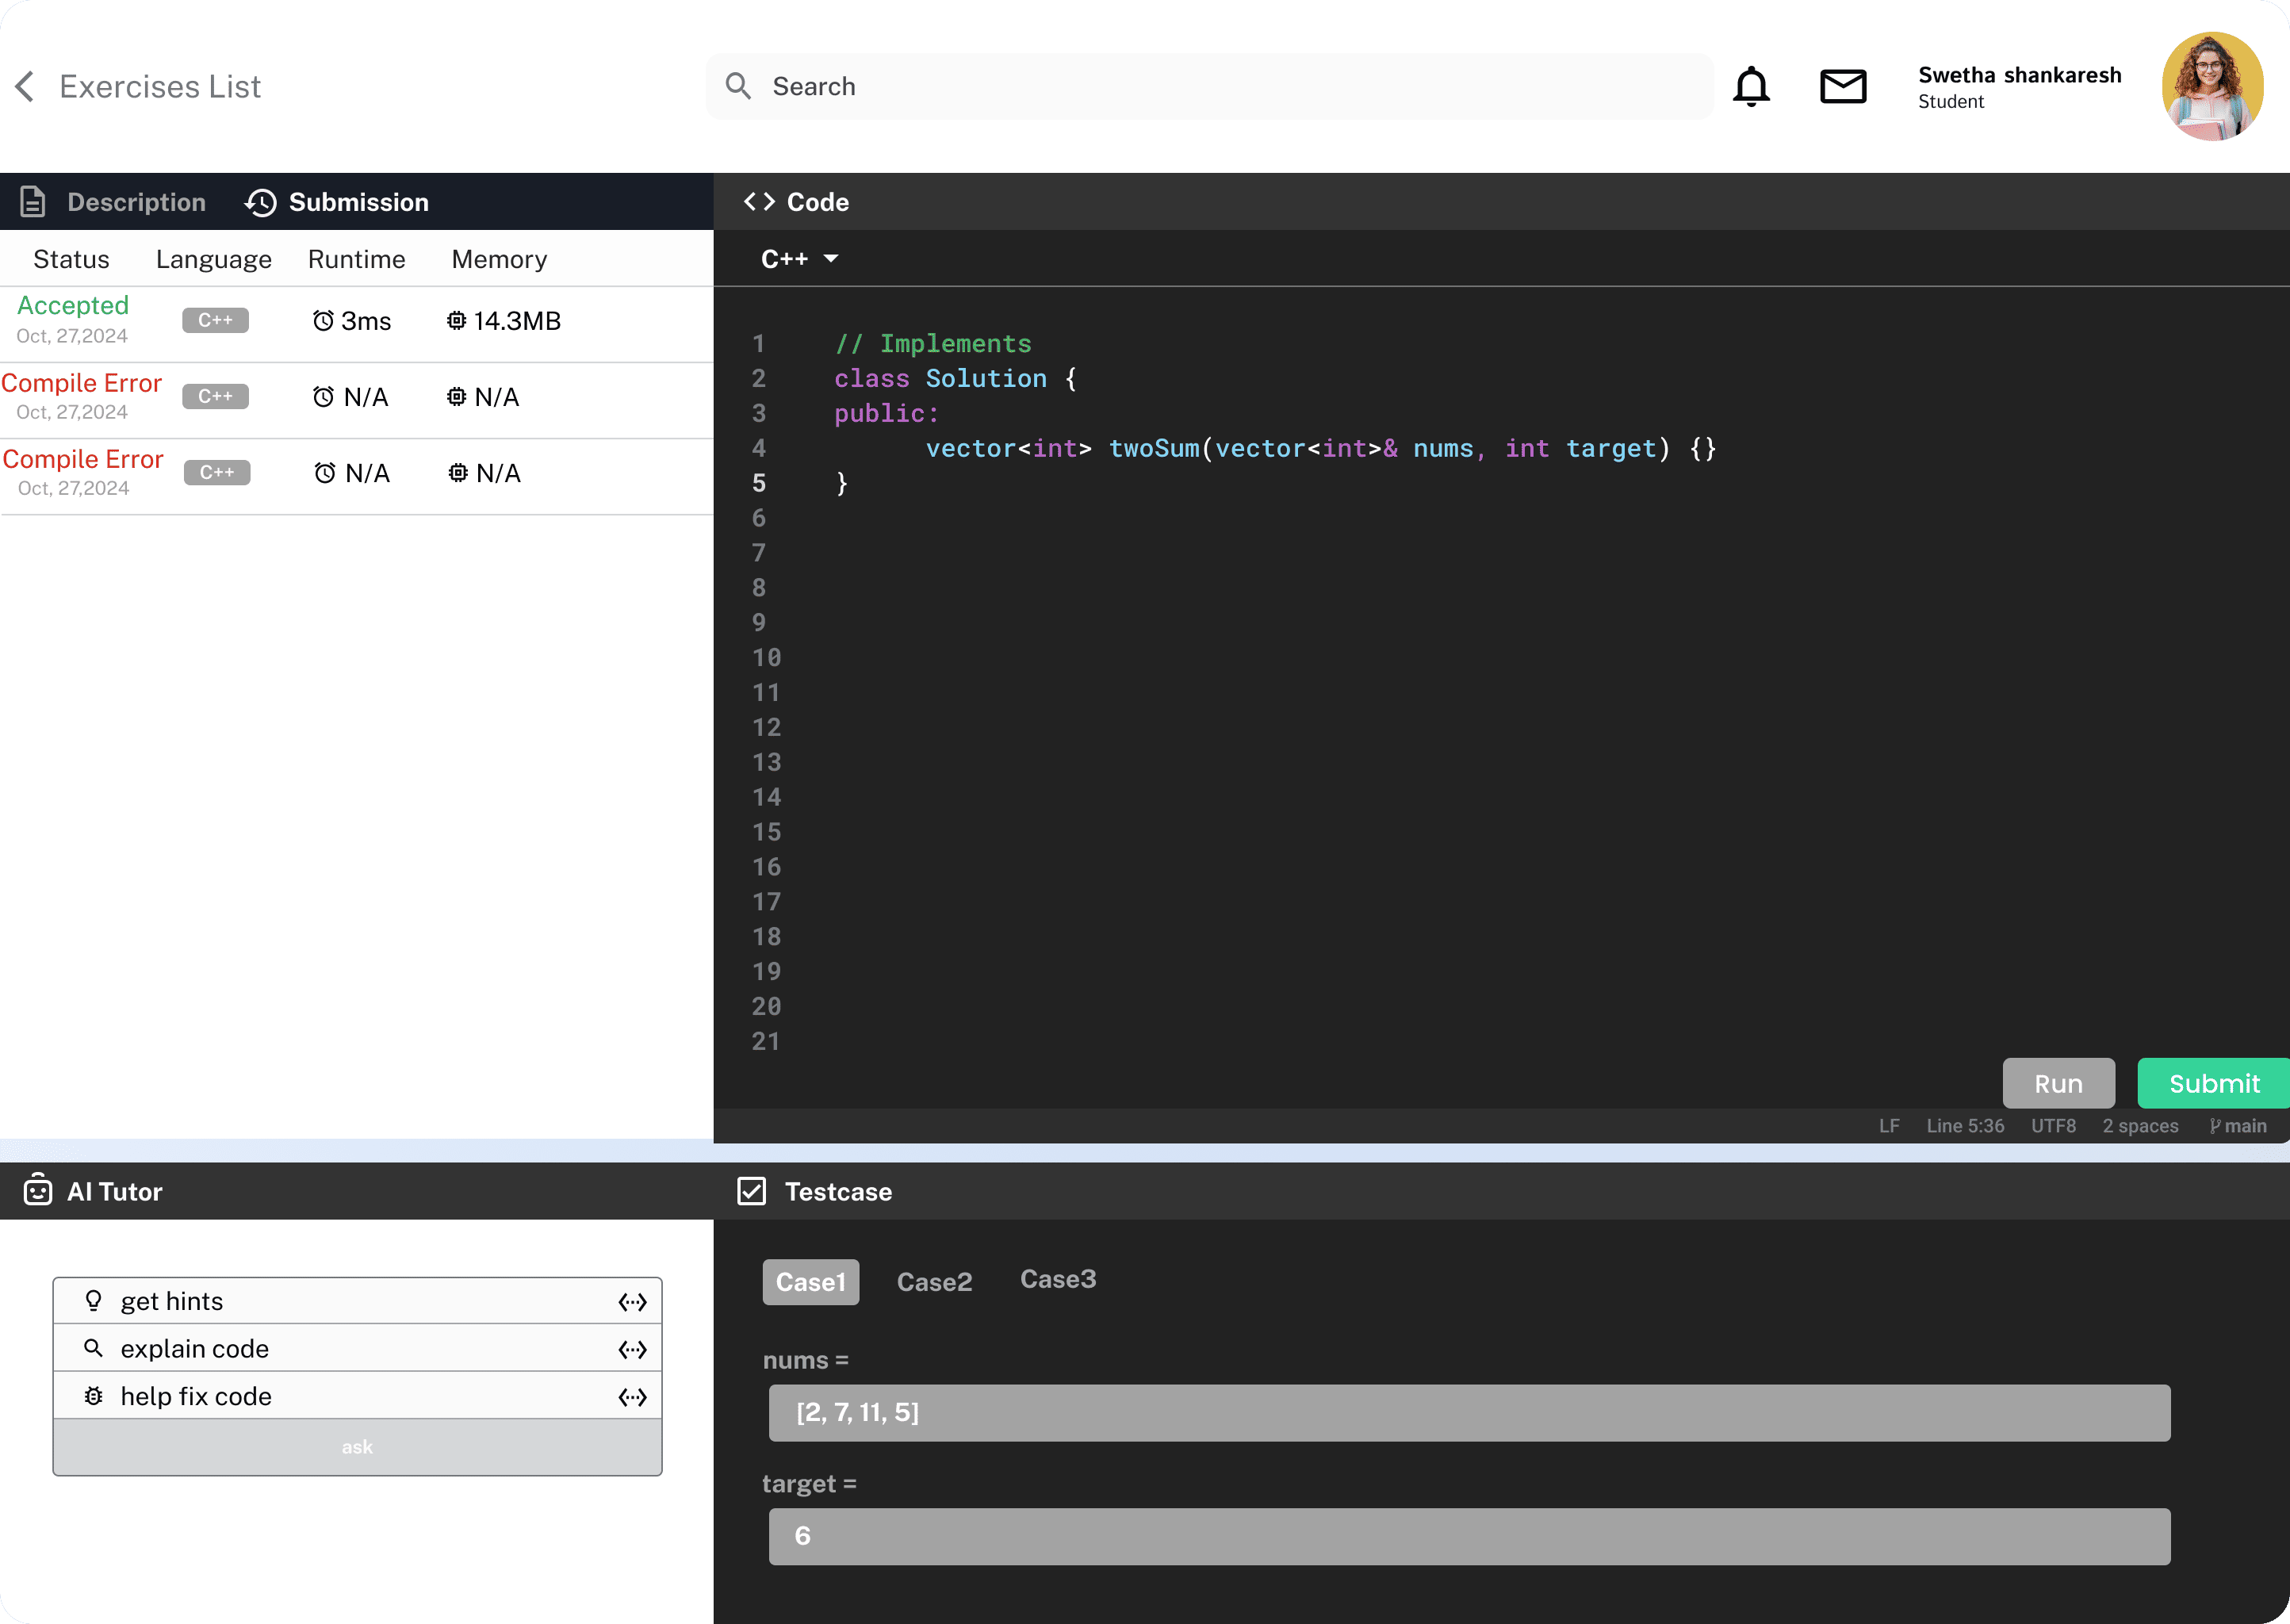
\includegraphics[width=0.7\linewidth]{Images/Anh/UI_Practice_submission.png}
    \caption{Lịch sử submission}
    \label{fig:enter-label}
\end{figure}
\subsection{AI Tutor}
Giao diện AI Tutor được thiết kế gồm ba chức năng chính như sau: cung cấp gợi ý (Get Hints), sửa lỗi (Fix Bug), và giải thích code (Explain Code). 
\begin{figure}[H]
    \centering
    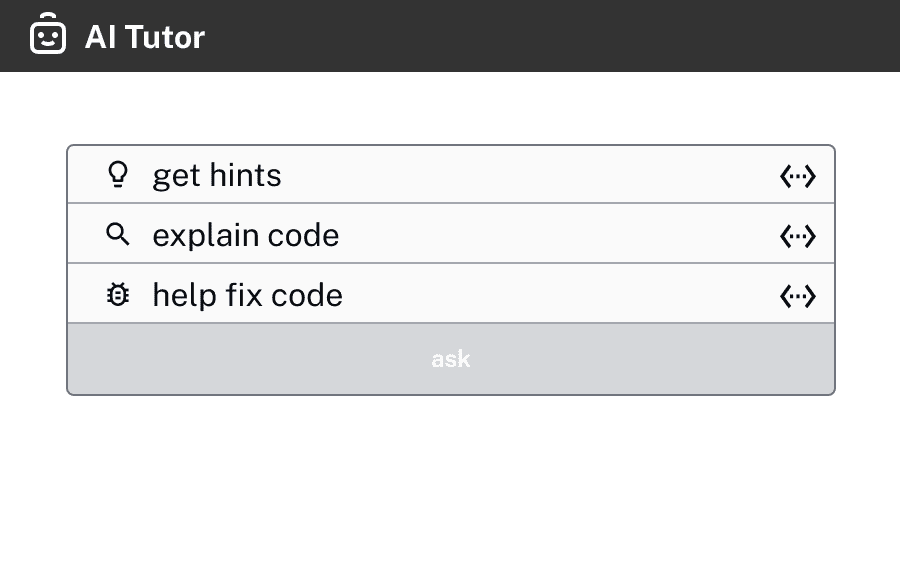
\includegraphics[width=0.7\linewidth]{Images/Anh/UI_AI_tutor.png}
    \caption{Các tính năng của AI Tutor}
    \label{fig:enter-label}
\end{figure}
Trong phần giải thích code, người dùng có thể chọn đoạn mã muốn hiểu rõ hơn; AI Tutor sẽ cung cấp giải thích tổng quát cho đoạn mã đó, và khi người dùng di chuột lên từng dòng, một popup sẽ hiển thị giải thích chi tiết cho từng dòng.
\begin{figure}[H]
    \centering
    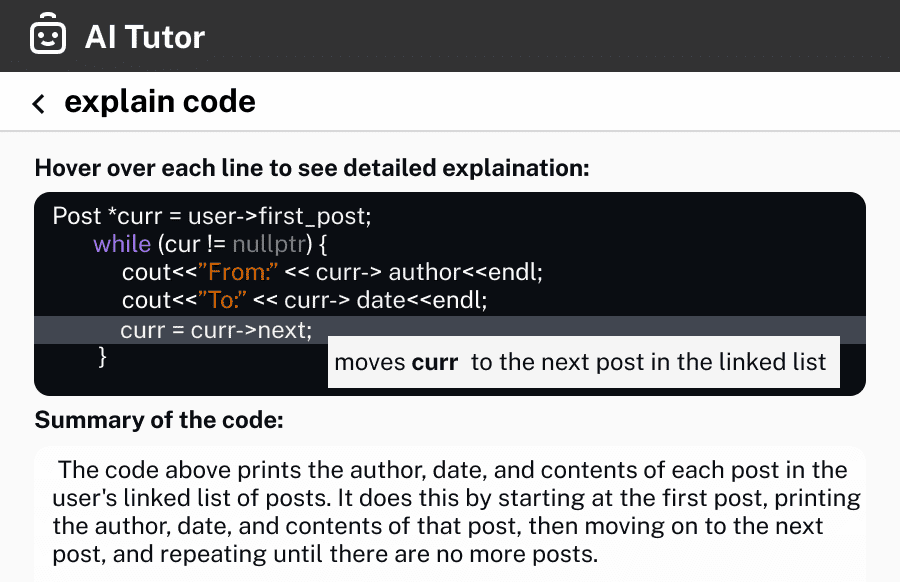
\includegraphics[width=0.7\linewidth]{Images/Anh/UI_AI_explain_code.png}
    \caption{Giải thích từng dòng code}
    \label{fig:enter-label}
\end{figure}
Đối với chức năng sửa lỗi, khi người dùng gặp lỗi trong quá trình compile code, AI Tutor sẽ phân tích và giải thích chi tiết nguyên nhân lỗi, đồng thời đề xuất cách khắc phục, giúp người dùng học hỏi từ lỗi sai của mình.
\begin{figure}[H]
    \centering
    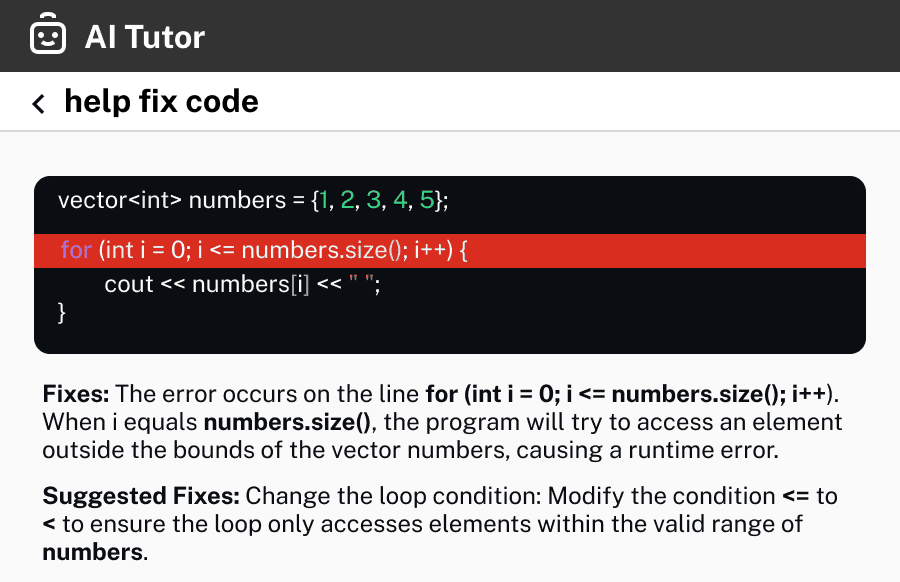
\includegraphics[width=0.7\linewidth]{Images/Anh/UI_help_fix_code.png}
    \caption{Hỗ trợ sửa lỗi}
    \label{fig:enter-label}
\end{figure}
Khi người dùng cần gợi ý cho bài tập, họ có thể nhấn nút "Get Hints" để nhận những hướng dẫn hữu ích; nếu chưa rõ, AI Tutor còn có thể đưa ra ví dụ minh họa giúp họ hiểu rõ hơn. 
\begin{figure}[H]
    \centering
    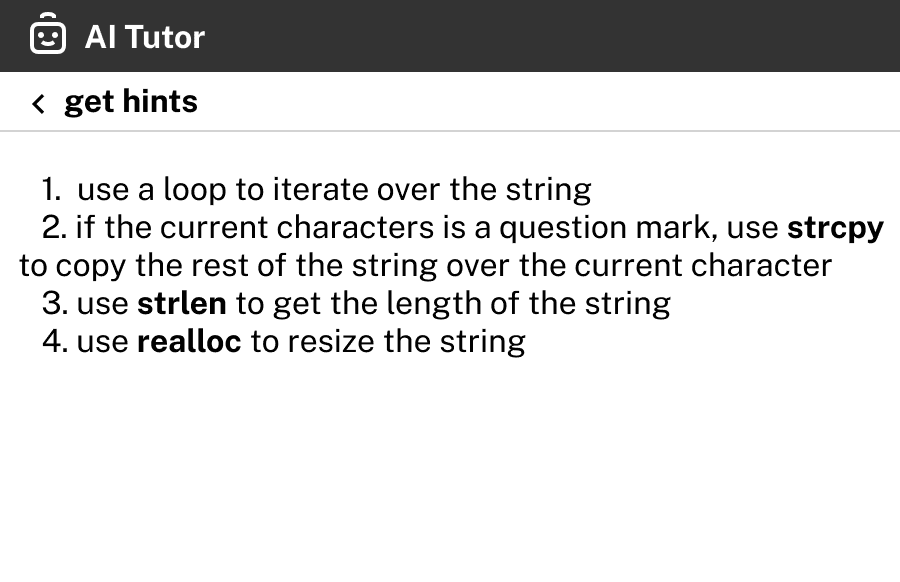
\includegraphics[width=0.7\linewidth]{Images/Anh/UI_AI_get_hints.png}
    \caption{Cung cấp gợi ý cho bài tập}
    \label{fig:enter-label}
\end{figure}
\subsection{Progress Tracking}
\begin{figure}[H]
    \centering
    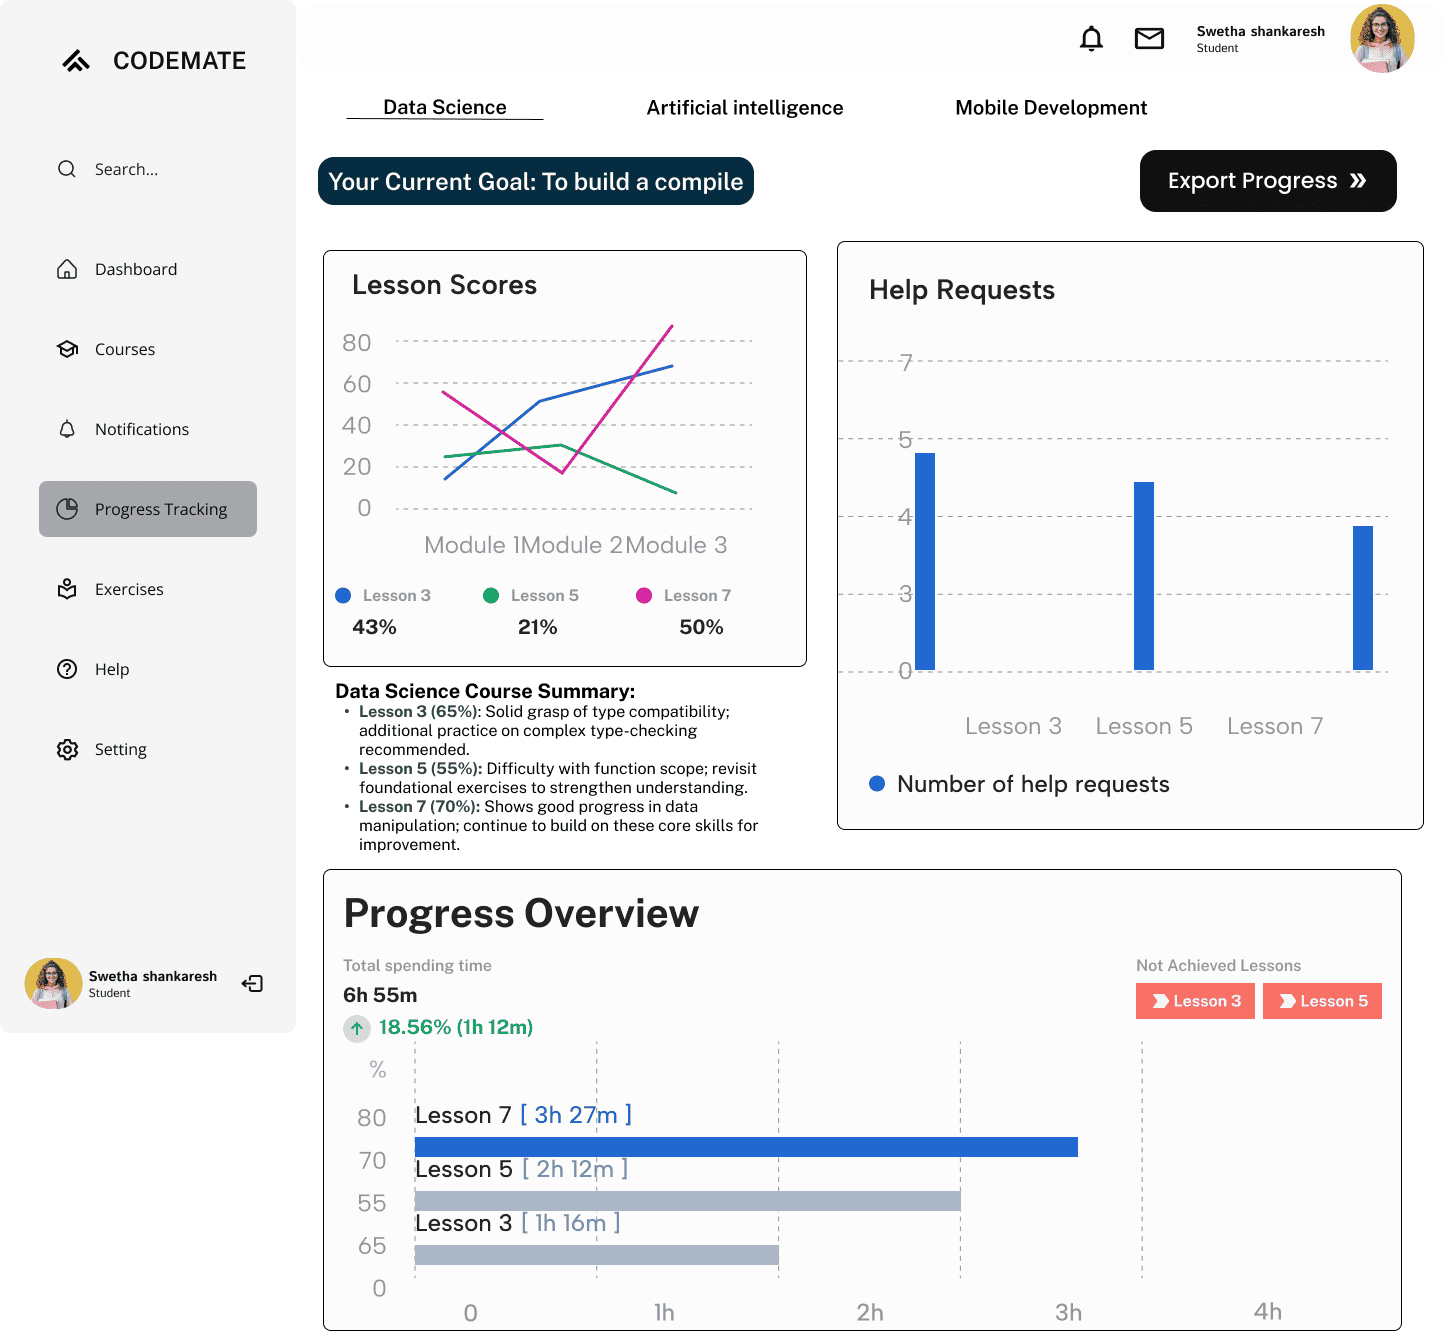
\includegraphics[width=1\linewidth]{Images/figmaDesign/Progress Tracking.png}
    \caption{Progress Tracking Page}
    \label{fig:enter-label}
\end{figure}
Trang Progress Tracking ghi lại tiến độ học tập của sinh viên theo từng môn học, bao gồm 3 biểu đồ chính: 
\begin{enumerate}
    \item \textbf{Biểu Đồ Đánh Giá Điểm Số Theo Lesson (Biểu đồ đường)}
    \begin{itemize}
        \item\textbf{X-Axis:} Tên module (1, 2, 3).
\item\textbf{Y-Axis:} Điểm số (từ 0 đến 100\%).
\item\textbf{Màu của đường biểu đồ:} Lesson(3,5,7)
\item\textbf{Đơn vị:} Phần trăm (\%).
\item\textbf{Ý Nghĩa:} Biểu đồ này cho phép sinh viên thấy tỷ lệ hoàn thành mục tiêu của từng module theo lesson và dễ dàng nhận ra lesson nào đạt hoặc chưa đạt yêu cầu, bị khó khăn ở module nào. 

    \end{itemize}
        \item \textbf{Biểu Đồ Theo Dõi Số Lượng Vấn Đề hoặc Yêu Cầu Trợ Giúp (Biểu đồ cột)}
    \begin{itemize}
        \item\textbf{X-Axis:} Tên lesson (1, 2, 3).
\item\textbf{Y-Axis:} Số lần sinh viên yêu cầu trợ giúp (Đếm số lần yêu cầu trợ giúp tới AI).
\item\textbf{Đơn vị:} Lần (Số lần hỏi).
\item\textbf{Ý Nghĩa:} Biểu đồ này ghi nhận độ khó của từng bài tập, giúp hệ thống nhận biết các phần cần được cải thiện hoặc các bài tập khó để review lại cho giáo viên hoặc sinh viên cần chú trọng học lại.
    \end{itemize}
            \item \textbf{Biểu Đồ Tổng Quan Tiến Độ Học (Progress Overview) (Biểu đồ cột)}
    \begin{itemize}
        \item\textbf{X-Axis:} Thời gian (Số giờ học).
\item\textbf{Y-Axis:} Tỷ lệ hoàn thành (\%) của lesson.
\item\textbf{Đơn vị:} Phần trăm (\%) hoàn thành lesson.
\item\textbf{Ý Nghĩa:} Cho thấy tiến độ tổng thể của sinh viên, giúp họ nhận ra tốc độ học của mình và đối chiếu với lộ trình học ban đầu.
    \end{itemize}
\end{enumerate}

\chapter{Hiện thực}

\section{Kiến trúc Frontend}

Frontend được xây dựng bằng VueJS, tích hợp Vuetify và Tailwind CSS để cung cấp giao diện người dùng trực quan, hiện đại và dễ sử dụng.

\begin{verbatim}
    CODEMATE-FE [WSL: UBUNTU]
    |-- .vite
    |-- dist
    |-- node_modules
    |-- public
    |-- src
    |   |-- assets
    |   |-- common
    |   |   |-- api.service.ts
    |   |   |-- config.ts
    |   |-- components
    |   |-- composables
    |   |-- constants
    |   |-- layouts
    |   |-- modals
    |   |-- pages
    |   |-- plugins
    |   |-- router
    |   |-- services
    |   |-- stores
    |   |-- types
    |   |-- utils
    |   |-- App.vue
    |   |-- auto-imports.d.ts
    |   |-- components.d.ts
    |   |-- global.css
    |   |-- main.ts
    |   |-- typed-router.d.ts
    |   |-- vite-env.d.ts
    |-- .browserslistrc
    |-- .editorconfig
    |-- .env
    |-- .eslintrc-auto-import.json
    \end{verbatim}

\subsection*{Hệ thống thiết kế (Design System)}

Hệ thống thiết kế được triển khai với mục tiêu cung cấp một giao diện người dùng nhất quán, dễ sử dụng và dễ mở rộng. Hệ thống này bao gồm các thành phần chính sau:

\subsubsection*{Typography}
Typography được xây dựng trên cơ sở font chữ Public Sans, với nhiều kích cỡ và độ đậm khác nhau để phục vụ các nhu cầu hiển thị khác nhau. Font chữ này được chọn vì dễ đọc, phù hợp với các thiết kế hiện đại và hỗ trợ đa ngôn ngữ. Các cấp độ bao gồm:

\begin{itemize}
    \item \textbf{Heading}: Từ Heading 1 (48px, Bold) đến Heading 4 (24px, Semibold).
    \item \textbf{Body Text}: Các cấp độ từ Large đến Small, sử dụng độ đậm từ Regular đến Bold, kích thước từ 10px đến 20px.
\end{itemize}

\begin{figure}[H]
    \centering
    \includegraphics[scale=0.3]{Images/Implement/Typography.png}
    \caption{Hệ thống Typography sử dụng trong ứng dụng}
\end{figure}

\subsubsection*{Bảng màu (Color Palette)}
Bảng màu được thiết kế để mang lại sự nhất quán và dễ nhận biết trong giao diện người dùng. Bảng màu chính bao gồm các màu \textbf{Primary}, \textbf{Secondary}, và các trạng thái như \textbf{Error}, \textbf{Warning}, \textbf{Neutral}, \textbf{Success}. Mỗi màu được chia thành các sắc độ từ nhạt (25, 50) đến đậm (900, 950), nhằm đảm bảo khả năng hiển thị tốt trong các trường hợp sử dụng khác nhau.

\begin{itemize}
    \item \textbf{Primary}: Dùng cho các thành phần chính như nút bấm và tiêu đề.
    \item \textbf{Secondary}: Dùng cho các chi tiết phụ hoặc nhấn mạnh nội dung.
    \item \textbf{Error, Warning, Success}: Dùng để phản hồi trạng thái của hệ thống.
\end{itemize}

\begin{figure}[H]
    \centering
    \includegraphics[scale=0.15]{Images/Implement/Colors.jpg}
    \caption{Bảng màu được sử dụng trong ứng dụng}
\end{figure}

Hệ thống này được tích hợp với Tailwind CSS, giúp tự động hóa việc áp dụng các quy tắc thiết kế (design tokens) vào mã nguồn. Điều này làm giảm thiểu lỗi thiết kế, đồng thời đảm bảo giao diện nhất quán trong toàn bộ ứng dụng.

\section{Kiến trúc Backend}

Backend được phát triển với FastAPI, kết hợp với PostgreSQL để lưu trữ dữ liệu. Kiến trúc hệ thống được tổ chức theo các thành phần chính:

\begin{itemize}
    \item Repository
    \item Provider
    \item Controller
    \item Schemas
    \item Models
    \item API
\end{itemize}
\newpage
\begin{verbatim}
    EDUMIND [WSL: UBUNTU]
    |-- alembic
    |   |-- script.py.mako
    |-- core
    |-- data
    |-- docker
    |-- docs
    |-- dumps
    |-- machine
    |   |-- __pycache__
    |   |-- api
    |   |-- controllers
    |   |-- models
    |   |-- providers
    |   |-- repositories
    |   |-- schemas
    |   |-- services
    |   |-- server.py
    |-- migrations
    |-- static
    |-- tasks
    |-- templates
    |-- utils
    |-- .env
    |-- .gitignore
    |-- .python-version
    |-- alembic.ini
    |-- main.py
    |-- Makefile
    |-- poetry.lock
    |-- pyproject.toml
    |-- README.md
    \end{verbatim}

\textbf{1. Repository} 

Repository chịu trách nhiệm quản lý các thao tác liên quan đến dữ liệu trong hệ thống. Đây là nơi thực hiện các logic liên quan đến việc truy vấn, lưu trữ và cập nhật dữ liệu từ cơ sở dữ liệu PostgreSQL.

Đặc điểm chính:

\begin{itemize}
    \item Tách biệt logic truy xuất dữ liệu khỏi các thành phần khác
    \item Hỗ trợ các thao tác CRUD (Create, Read, Update, Delete)
\end{itemize}

Ví dụ: Repository sẽ xử lý các tác vụ như:

\begin{itemize}
    \item Truy vấn thông tin sinh viên và giảng viên
    \item Cập nhật tiến độ học tập
    \item Xóa thông tin khóa học khi cần thiết
\end{itemize}

\textbf{2. Provider} 

Provider chịu trách nhiệm xử lý các logic nghiệp vụ (business logic). Đây là nơi các phép toán và xử lý phức tạp được thực hiện trước khi trả kết quả cho Controller hoặc người dùng.

Đặc điểm chính:

\begin{itemize}
    \item Không phụ thuộc vào giao diện hoặc nguồn dữ liệu cụ thể
    \item Tập trung vào logic nghiệp vụ và các phép toán quan trọng
\end{itemize}

Ví dụ: Provider sẽ:

\begin{itemize}
    \item Phân tích mục tiêu học tập của sinh viên để đề xuất bài học
    \item Tự động tạo bài học dựa trên nội dung được giảng viên cung cấp
\end{itemize}
 
\textbf{3. Controller} 

Controller là nơi tiếp nhận các yêu cầu từ người dùng thông qua API, sau đó phối hợp với Provider và Repository để thực hiện các chức năng tương ứng.

Đặc điểm chính:

\begin{itemize}
    \item Giao tiếp trực tiếp với frontend thông qua các endpoint API
    \item Chuyển đổi dữ liệu giữa frontend và các thành phần backend
\end{itemize}

Ví dụ: Controller xử lý:

\begin{itemize}
    \item Yêu cầu đăng nhập và xác thực người dùng
    \item Truy xuất danh sách khóa học và chi tiết khóa học
    \item Nhận mục tiêu học tập từ sinh viên và gửi đến Provider để xử lý
\end{itemize}

\section{Quá trình triển khai hệ thống}
\subsection*{Triển khai hệ thống}

Hệ thống được triển khai hoàn toàn trên nền tảng Render, áp dụng cho cả thành phần frontend và backend. Việc sử dụng một nền tảng duy nhất cho toàn bộ hệ thống giúp đơn giản hóa quy trình CI/CD, quản lý tài nguyên tập trung và tối ưu hóa hiệu suất giao tiếp giữa các thành phần.

\textbf{Frontend:} Ứng dụng Vue.js được triển khai dưới dạng dịch vụ tĩnh (Static Site) trên Render với cấu hình tự động xây dựng và triển khai khi mã nguồn được cập nhật.

\par \textbf{Link deploy frontend:} \textcolor{blue}{\href{https://codemate-fe-n5h9.onrender.com/}{https://codemate-fe-n5h9.onrender.com/}}

\textbf{Backend:} API FastAPI được triển khai dưới dạng dịch vụ web (Web Service) trên Render, với Docker làm công nghệ đóng gói để đảm bảo tính nhất quán môi trường. Hệ thống sử dụng Poetry để quản lý các phụ thuộc Python, đảm bảo môi trường phát triển và triển khai đồng nhất.

\par \textbf{Link deploy backend:} \textcolor{blue}{\href{https://edumind-5qmn.onrender.com/}{https://edumind-5qmn.onrender.com/}}

\textbf{Quy trình triển khai chi tiết:}
% \begin{figure}[H]
% \centering
% \includegraphics[width=0.85\linewidth]{Images/Implement/DeploymentProcess.png}
% \caption{Quy trình triển khai hệ thống}
% \label{fig}
% \end{figure}
\begin{enumerate}
\item \textbf{Chuẩn bị môi trường phát triển:}
\begin{itemize}
\item Thiết lập môi trường phát triển cục bộ với đầy đủ công cụ cần thiết như Node.js, npm, Python 3.10, và Poetry.
\item Cài đặt các IDE và công cụ phát triển như Visual Studio Code, PyCharm, và Git.
\item Thiết lập hệ thống kiểm soát phiên bản sử dụng GitHub để quản lý mã nguồn và hỗ trợ làm việc nhóm.
\end{itemize}
\item \textbf{Phát triển frontend:}
\begin{itemize}
    \item Sử dụng Vue 3 và Vuetify để xây dựng giao diện người dùng.
    \item Triển khai các component UI theo thiết kế đã được phê duyệt.
    \item Tích hợp các thư viện hỗ trợ như Axios cho việc gọi API, Pinia cho quản lý trạng thái.
    \item Thực hiện tối ưu hóa hiệu suất và khả năng đáp ứng trên các thiết bị khác nhau.
\end{itemize}

\item \textbf{Phát triển backend:}
\begin{itemize}
    \item Xây dựng API sử dụng FastAPI theo kiến trúc Repository-Provider-Controller.
    \item Thiết lập kết nối và tương tác với cơ sở dữ liệu PostgreSQL.
    \item Tích hợp các dịch vụ bên ngoài như Gemini API, Google Authentication.
    \item Phát triển các module xử lý nghiệp vụ chính như quản lý người dùng, quản lý khóa học, đề xuất học tập, và tạo bài tập.
\end{itemize}

\item \textbf{Kiểm thử hệ thống:}
\begin{itemize}
    \item Thực hiện kiểm thử đơn vị cho các thành phần riêng lẻ.
    \item Kiểm thử tích hợp để đảm bảo các thành phần phối hợp tốt với nhau.
    \item Kiểm thử chức năng để xác nhận các tính năng hoạt động đúng theo yêu cầu.
    \item Kiểm thử hiệu suất để đánh giá khả năng đáp ứng và xử lý tải của hệ thống.
\end{itemize}

\item \textbf{Triển khai trên môi trường cloud:}
\begin{itemize}
    \item Thiết lập môi trường cloud trên Render cho frontend và backend.
    \item Cấu hình các biến môi trường và thiết lập bảo mật.
    \item Thiết lập quy trình CI/CD để tự động hóa việc build và deploy khi có thay đổi trong mã nguồn.
    \item Cài đặt và cấu hình cơ sở dữ liệu PostgreSQL trên nền tảng đám mây.
\end{itemize}

% \item \textbf{Giám sát và bảo trì:}
% \begin{itemize}
%     \item Thiết lập hệ thống giám sát để theo dõi hiệu suất và phát hiện sự cố.
%     \item Triển khai quy trình cập nhật và bảo trì định kỳ.
%     \item Phân tích dữ liệu sử dụng để cải thiện trải nghiệm người dùng và tối ưu hóa hiệu suất.
%     \item Xử lý các vấn đề và cải tiến hệ thống dựa trên phản hồi từ người dùng.
% \end{itemize}
\end{enumerate}
\textbf{Các công nghệ được sử dụng trong triển khai:}
\begin{table}[H]
\centering
\caption{Các công nghệ sử dụng trong quá trình triển khai}
\begin{tabularx}{\textwidth}{|l|X|}
\hline
\textbf{Lĩnh vực} & \textbf{Công nghệ} \\ \hline
Frontend & Vue 3, Vuetify, Tailwind CSS, Pinia, Axios \\ \hline
Backend & FastAPI, SQLAlchemy, Pydantic, LangChain, Alembic \\ \hline
Cơ sở dữ liệu & PostgreSQL, Redis (cache) \\ \hline
AI & OpenAI API (GPT-4o), Google Gemini API \\ \hline
Triển khai & Render (Frontend, Backend), GitHub Actions (CI/CD) \\ \hline
% Giám sát & Sentry, Prometheus, Grafana \\ \hline
\end{tabularx}

\label{table}
\end{table}
% \textbf{Kết quả triển khai:}
% Sau khi hoàn thành quá trình triển khai, hệ thống đã được đưa vào vận hành thử nghiệm với một nhóm người dùng ban đầu. Kết quả thu được rất khả quan, với thời gian phản hồi nhanh và trải nghiệm người dùng mượt mà. Hệ thống đã xử lý được hơn 500 yêu cầu đồng thời trong các đợt kiểm tra tải, đảm bảo khả năng phục vụ số lượng lớn người dùng trong tương lai.
% Các tính năng chính như đề xuất lộ trình học tập, tạo bài tập tự động, và gia sư AI đều hoạt động tốt trong môi trường sản xuất, với thời gian phản hồi trung bình cho các yêu cầu AI dưới 5 giây, đáp ứng yêu cầu về hiệu suất đề ra.
% \begin{figure}[H]
% \centering
% \includegraphics[width=0.85\linewidth]{Images/Implement/SystemPerformance.png}
% \caption{Biểu đồ hiệu suất hệ thống sau khi triển khai}
% \label{fig}
% \end{figure}
% Quá trình triển khai hệ thống đã diễn ra suôn sẻ, với các vấn đề phát sinh được xử lý kịp thời. Hệ thống hiện đang hoạt động ổn định và sẵn sàng cho việc mở rộng quy mô trong tương lai.
% \section{Các chức năng đã được thực hiện}

% Dưới đây là các chức năng đã được thực hiện trong hệ thống học tập trực tuyến thông minh. Các chức năng này được phân chia theo từng module và vai trò của người dùng trong hệ thống.

% \subsection{Quản lý tài khoản (Thành viên đảm nhiệm: Phạm Thi)}
% Module này cung cấp các chức năng liên quan đến đăng nhập, xác thực và quản lý thông tin cá nhân của người dùng.
% \begin{itemize}[label=--]
%     \item Đăng nhập vào hệ thống bằng email/mật khẩu hoặc tài khoản Google (Role: Sinh viên, Giảng viên, Quản trị viên).
%     \item Làm mới token xác thực khi phiên đăng nhập hết hạn (Role: Sinh viên, Giảng viên, Quản trị viên).
%     \item Xác minh email và gửi lại mã xác minh nếu cần (Role: Sinh viên, Giảng viên, Quản trị viên).
%     \item Đặt lại mật khẩu khi quên mật khẩu (Role: Sinh viên, Giảng viên, Quản trị viên).
%     \item Cập nhật thông tin cá nhân (tên, ngày sinh, ảnh đại diện) (Role: Sinh viên, Giảng viên, Quản trị viên).
%     \item Xem thông tin hồ sơ cá nhân (ID, tên, email, MSSV/MSCB, ngày sinh, vai trò) (Role: Sinh viên, Giảng viên, Quản trị viên).
% \end{itemize}

% \begin{figure}[H]
%     \centering
%     \includegraphics[width=0.9\linewidth]{images/Quan_ly_tai_khoan/authenFlow.drawio.png}
%     \caption{Flow Định danh tài khoản}
%     \label{fig:enter-label}
% \end{figure}

% \subsection{Quản lý khóa học (Thành viên đảm nhiệm: Phạm Thi/Tuấn Anh)}
% Module này hỗ trợ quản lý thông tin khóa học, bao gồm tạo, xem, cập nhật và xóa dữ liệu liên quan.
% \begin{itemize}[label=--]
%     \item Xem danh sách khóa học (đã đăng ký hoặc đang phụ trách, hỗ trợ phân trang và tìm kiếm) (Role: Sinh viên, Giảng viên).
%     \item Xem chi tiết khóa học (số lượng sinh viên, bài học, bài tập, tài liệu, tiến độ học tập) (Role: Sinh viên, Giảng viên).
%     \item Xem thông tin Giảng viên của khóa học (Role: Sinh viên).
%     \item Cập nhật mục tiêu học tập và ảnh khóa học (Role: Giảng viên).
%     \item Tạo khóa học mới (đơn lẻ hoặc nhiều khóa) (Role: Quản trị viên).
%     \item Cập nhật thông tin khóa học (tên, tín chỉ, học kỳ) (Role: Quản trị viên).
%     \item Xóa khóa học cùng dữ liệu liên quan (Role: Quản trị viên).
%     \item Xem danh sách khóa học có sẵn của HCMUT (Role: Quản trị viên).
%     \item Xem khóa học truy cập gần đây nhất qua dashboard (Role: Sinh viên).
% \end{itemize}

% \subsection{Quản lý bài học (Thành viên đảm nhiệm: Phạm Thi/Tuấn Anh)}
% Module này cho phép tạo, chỉnh sửa và quản lý bài học trong khóa học.
% \begin{itemize}[label=--]
%     \item Xem danh sách bài học trong khóa học (Role: Sinh viên).
%     \item Tạo bài học mới (Role: Giảng viên).
%     \item Cập nhật bài học (tiêu đề, mô tả, mục tiêu học tập) (Role: Giảng viên).
%     \item Xóa bài học cùng tài liệu liên quan (Role: Giảng viên).
%     \item Thêm tài liệu vào bài học (Role: Giảng viên).
%     \item Xem chi tiết bài học và danh sách tài liệu liên quan (Role: Giảng viên).
% \end{itemize}

% \subsection{Quản lý bài tập (Thành viên đảm nhiệm: Tuấn Anh)}
% Module này hỗ trợ quản lý bài tập dạng quiz và lập trình, bao gồm tạo, xem và nộp bài.
% \begin{itemize}[label=--]
%     \item Xem danh sách bài tập trong khóa học (chỉ bài tập đã mở) (Role: Sinh viên).
%     \item Xem chi tiết bài tập dạng quiz hoặc lập trình (câu hỏi, yêu cầu, test cases) (Role: Sinh viên, Giảng viên).
%     \item Tạo bài tập dạng quiz hoặc lập trình (Role: Giảng viên).
%     \item Cập nhật thông tin bài tập dạng quiz hoặc lập trình (Role: Giảng viên).
%     \item Xóa bài tập dạng quiz hoặc lập trình (Role: Giảng viên).
%     \item Gửi câu hỏi tới trợ lý lập trình và xem lịch sử hội thoại (Role: Sinh viên).
%     \item Nộp bài quiz và xóa câu trả lời để làm lại (Role: Sinh viên).
%     \item Xem danh sách sự kiện bài tập sắp tới qua lịch học (Role: Sinh viên, Giảng viên).
% \end{itemize}

% \subsection{Quản lý lộ trình học tập (Thành viên đảm nhiệm: Phạm Thi/Tuấn Anh)}
% Module này cung cấp các chức năng liên quan đến lộ trình học tập cá nhân hóa và bài học đề xuất.
% \begin{itemize}[label=--]
%     \item Xem lộ trình học tập cá nhân hóa và danh sách bài học đề xuất (Role: Sinh viên).
%     \item Xóa lộ trình học tập cá nhân (Role: Sinh viên).
%     \item Xem chi tiết bài học đề xuất (tiêu đề, mục tiêu, nội dung, tiến độ) (Role: Sinh viên).
%     \item Đánh dấu hoặc bỏ đánh dấu bài học đề xuất (Role: Sinh viên).
%     \item Yêu cầu tạo lộ trình học tập dựa trên mục tiêu và khóa học (Role: Sinh viên).
%     \item Tái tạo nội dung bài học dựa trên vấn đề đã xác định (Role: Sinh viên).
%     \item Nhận gợi ý mục tiêu học tập từ hệ thống (Role: Sinh viên).
%     \item Xem tài liệu của module trong lộ trình học tập (Role: Sinh viên).
%     \item Tạo bài quiz dựa trên nội dung module (Role: Sinh viên).
% \end{itemize}

% \subsection{Theo dõi tiến độ học tập (Thành viên đảm nhiệm: Phạm Thi/Tuấn Anh)}
% Module này hỗ trợ theo dõi và đánh giá tiến độ học tập của sinh viên.
% \begin{itemize}[label=--]
%     \item Nhận đánh giá tiến độ học tập theo chuẩn Rubric (Role: Sinh viên).
%     \item Cập nhật thời gian học cho bài học đề xuất (Role: Sinh viên).
%     \item Xem phân tích tiến độ học tập trong khóa học hoặc bài học cụ thể (Role: Sinh viên).
%     \item Xem điểm số của sinh viên trong khóa học (tên, email, MSSV, điểm trung bình) (Role: Giảng viên).
%     \item Xem điểm chi tiết của một bài tập cụ thể (Role: Giảng viên).
% \end{itemize}

% \subsection{Quản lý phản hồi (Thành viên đảm nhiệm: Phạm Thi)}
% Module này cho phép gửi, xem và quản lý phản hồi trong hệ thống.
% \begin{itemize}[label=--]
%     \item Gửi phản hồi về hệ thống hoặc khóa học (tiêu đề, mô tả, đánh giá) (Role: Sinh viên, Giảng viên).
%     \item Xem danh sách phản hồi (lọc theo tháng, năm, trạng thái, khóa học) (Role: Giảng viên, Quản trị viên).
%     \item Cập nhật trạng thái phản hồi (pending, in\_progress, resolved) (Role: Quản trị viên).
%     \item Xóa phản hồi khỏi hệ thống (Role: Quản trị viên).
% \end{itemize}

% \subsection{Quản lý người dùng (Thành viên đảm nhiệm: Phạm Thi)}
% Module này cung cấp các chức năng quản lý thông tin và trạng thái người dùng trong hệ thống.
% \begin{itemize}[label=--]
%     \item Tạo người dùng mới (sinh viên, Giảng viên, quản trị viên) (Role: Quản trị viên).
%     \item Đếm số lượng người dùng (tổng hoặc theo vai trò) (Role: Quản trị viên).
%     \item Xem danh sách tất cả người dùng (lọc theo vai trò, trạng thái, tìm kiếm) (Role: Quản trị viên).
%     \item Xem thông tin chi tiết của một người dùng cụ thể (Role: Quản trị viên).
%     \item Cập nhật trạng thái người dùng (bật/tắt) (Role: Quản trị viên).
% \end{itemize}

% \subsection{Quản lý nhật ký đăng nhập (Thành viên đảm nhiệm: Phạm Thi)}
% Module này hỗ trợ theo dõi và ghi nhận hoạt động đăng nhập của người dùng.
% \begin{itemize}[label=--]
%     \item Xem danh sách nhật ký đăng nhập (ID người dùng, vai trò, thời gian) (Role: Quản trị viên).
%     \item Tạo bản ghi nhật ký đăng nhập mới (Role: Quản trị viên).
% \end{itemize}

% \subsection{Quản lý dashboard (Thành viên đảm nhiệm: Phạm Thi)}
% Module này cung cấp tổng quan hoạt động cho người dùng qua giao diện dashboard.
% \begin{itemize}[label=--]
%     \item Xem tổng quan hoạt động giảng dạy (số lượng khóa học, bài học, sinh viên, bài tập) (Role: Giảng viên).
%     \item Xem và thêm các hoạt động gần đây (tối đa 5 hoạt động) (Role: Sinh viên).
% \end{itemize}

% \subsection{Code Assistant (Thành viên đảm nhiệm: Phương Nam)}
% Module này hỗ trợ sinh viên trong việc lập trình và giải quyết các vấn đề liên quan đến mã nguồn.
% \begin{itemize}[label=--]
%     \item Gợi ý mã nguồn dựa trên yêu cầu của sinh viên (Role: Sinh viên).
%     \item Tạo bài kiểm tra lập trình dựa trên nội dung module (Role: Sinh viên).
%     \item Hỗ trợ kiểm tra mã nguồn và đưa ra các gợi ý sửa lỗi (Role: Sinh viên).
%     \item Hướng dẫn sinh viên trong việc giải quyết các vấn đề lập trình (Role: Sinh viên).
%     \item Chatbot hỗ trợ sinh viên trong việc lập trình và giải quyết các vấn đề liên quan đến mã nguồn (Role: Sinh viên).
% \end{itemize}
% \section{Giới thiệu chi tiết về các chức năng chính của hệ thống}
% Hệ thống học tập thông minh được thiết kế để hỗ trợ học sinh trong việc lập kế hoạch học tập và đánh giá tiến độ một cách hiệu quả. Với sự tích hợp của AI, hệ thống có khả năng phân tích dữ liệu học tập, tạo lộ trình cá nhân hóa và đưa ra các đánh giá chi tiết. Mục nội dung này sẽ tập trung vào các chức năng chính như sinh ra lộ trình học tập, đề xuất mục tiêu học tập, đánh giá kết quả học tập, tạo bài kiểm tra, và các tính năng bổ sung khác. \par 

% Sau đây là các nguyên tắc cơ bản trong việc thiết lập mục tiêu học tập và phương pháp đánh giá mà hệ thống áp dụng:

% \subsection{Nguyên tắc SMART trong việc thiết lập mục tiêu}
% Nguyên tắc SMART là một khung tiêu chuẩn được áp dụng rộng rãi trong việc thiết lập mục tiêu hiệu quả. Trong hệ thống của chúng tôi, mỗi mục tiêu học tập được đề xuất đều tuân theo năm tiêu chí của nguyên tắc SMART:

% \begin{itemize}
%     \item \textbf{Specific (Cụ thể)}: Mục tiêu phải rõ ràng và cụ thể, không mơ hồ. Ví dụ: ``Hiểu và áp dụng được các thuật toán sắp xếp'' thay vì ``Học về thuật toán''.
    
%     \item \textbf{Measurable (Đo lường được)}: Mục tiêu phải có thể đo lường được để đánh giá tiến độ. Ví dụ: ``Đạt điểm 8/10 trong bài kiểm tra về cấu trúc dữ liệu'' hoặc ``Hoàn thành 5 bài tập lập trình về đệ quy''.
    
%     \item \textbf{Achievable (Khả thi)}: Mục tiêu phải thực tế và có thể đạt được với các nguồn lực và thời gian hiện có. Mục tiêu quá tham vọng có thể dẫn đến nản chí.
    
%     \item \textbf{Relevant (Liên quan)}: Mục tiêu phải phù hợp với nội dung khóa học và kết quả học tập mong đợi. Ví dụ, đặt mục tiêu học sâu về machine learning sẽ không phù hợp cho một khóa học cơ bản về Python.
    
%     \item \textbf{Time-bound (Giới hạn thời gian)}: Mục tiêu phải có thời hạn cụ thể để tạo động lực và tính cấp bách. Ví dụ: ``Hoàn thành trước kỳ thi giữa kỳ'' hoặc ``Trong vòng 3 tuần''.
% \end{itemize}

% Trong API \texttt{/generate-student-goals}, AI sẽ tạo ra các mục tiêu học tập tuân thủ nguyên tắc SMART cho ba cấp độ học tập khác nhau: Struggling (khó khăn), Average (trung bình), và Advanced (nâng cao). Mỗi mục tiêu đều được giới hạn dưới 200 ký tự để đảm bảo tính súc tích và dễ nhớ.

% \subsection{Phương pháp Rubric-Based Assessment}
% Rubric-Based Assessment (Đánh giá dựa trên Rubric) là phương pháp đánh giá sử dụng các tiêu chí cụ thể và mức độ đạt được cho mỗi tiêu chí. Phương pháp này mang lại nhiều lợi ích:

% \begin{itemize}
%     \item \textbf{Tính khách quan}: Đánh giá dựa trên các tiêu chí rõ ràng, giảm thiểu tính chủ quan.
%     \item \textbf{Tính nhất quán}: Đảm bảo các học sinh được đánh giá theo cùng một tiêu chuẩn.
%     \item \textbf{Tính minh bạch}: Học sinh hiểu rõ họ được đánh giá như thế nào và cần cải thiện điều gì.
%     \item \textbf{Phản hồi có cấu trúc}: Cung cấp phản hồi chi tiết theo từng tiêu chí.
% \end{itemize}

% Trong hệ thống của chúng tôi, Rubric được áp dụng để đánh giá học sinh theo ba tiêu chí chính:
% \begin{enumerate}
%     \item \textbf{Kiến thức lý thuyết (Theoretical Knowledge)}: Đánh giá mức độ hiểu biết về lý thuyết dựa trên tiến độ trong các bài học liên quan đến khái niệm lý thuyết.
    
%     \item \textbf{Kỹ năng thực hành (Coding Skills)}: Đánh giá kỹ năng lập trình dựa trên việc hoàn thành các bài tập mã hóa. Nếu khóa học không bao gồm lập trình, tiêu chí này sẽ được thay thế bằng một kỹ năng thực hành khác phù hợp.
    
%     \item \textbf{Nỗ lực (Effort)}: Đánh giá sự cố gắng dựa trên thời gian học tập (time\_spent), số lượng bài học đã bắt đầu (status), và tiến độ tổng thể.
% \end{enumerate}

% Mỗi tiêu chí được đánh giá theo bốn mức độ: Excellent (Xuất sắc), Good (Tốt), Average (Trung bình), và Poor (Kém), với các miêu tả cụ thể cho mỗi mức độ.

% \subsection{Phương pháp đánh giá STAR}
% STAR là một phương pháp đánh giá cấu trúc được sử dụng rộng rãi trong giáo dục và phát triển nghề nghiệp. Trong hệ thống của chúng tôi, phương pháp STAR được áp dụng để đánh giá tiến độ học tập của học sinh một cách toàn diện. STAR bao gồm bốn thành phần:

% \begin{itemize}
%     \item \textbf{Situation (Tình huống)}: Mô tả bối cảnh học tập của học sinh, bao gồm tên, khóa học, và mối liên hệ với mục tiêu học tập.
    
%     \item \textbf{Task (Nhiệm vụ)}: Nêu rõ mục tiêu học tập của học sinh, nhấn mạnh tầm quan trọng của việc đạt được mục tiêu trước thời hạn (ví dụ: trước kỳ thi giữa kỳ).
    
%     \item \textbf{Action (Hành động)}: Liệt kê chi tiết các hành động học sinh đã thực hiện cho mỗi tiêu chí đánh giá (Kiến thức lý thuyết, Kỹ năng thực hành, Nỗ lực), dựa trên dữ liệu bài học (progress, time\_spent, objectives).
    
%     \item \textbf{Result (Kết quả)}: Đánh giá tiến độ tổng thể so với mục tiêu, phân tích theo từng tiêu chí, với nhận xét rõ ràng (on track/needs effort/at risk) và tham chiếu đến ngày hiện tại.
% \end{itemize}

% API \texttt{/student/\{courseId\}/assessment} sử dụng phương pháp STAR kết hợp với Rubric để tạo ra báo cáo đánh giá toàn diện cho học sinh, giúp họ hiểu rõ tiến độ học tập và những điểm cần cải thiện.

\section{Sinh ra lộ trình học tập}
Chức năng này chịu trách nhiệm tạo ra một lộ trình học tập cá nhân hóa dựa trên mục tiêu học tập của học sinh, nội dung khóa học và thời gian khả dụng. Quá trình được thực hiện qua ba giai đoạn chính:

\begin{enumerate}
    \item \textbf{Phân tích mục tiêu và thời gian}: Hàm \texttt{analyze\_goal\_and\_timeline} kiểm tra tính hợp lệ của mục tiêu (ví dụ: độ dài, tính liên quan) và xác định thời gian khả thi dựa trên ngày bắt đầu và kết thúc khóa học. Ví dụ mã nguồn:
    \begin{lstlisting}[language=Python]
async def analyze_goal_and_timeline(goal: str, course_start_date: datetime, ...):
    if len(goal) < 10:
        raise ApplicationException(message="Goal is too short...")
    prompt = f"..."
    chunking_manager = ChunkingManager(
        provider="gemini",
        gemini_model_name="gemini-2.0-flash-lite",
        max_tokens_per_chunk=15000,
        temperature=0.7,
        max_output_tokens=8000
    )
    response = chunking_manager.call_llm_api(prompt, "You are an expert in goal validation and timeline analysis.")
    \end{lstlisting}

    \item \textbf{Lựa chọn bài học liên quan}: Hàm \texttt{select\_relevant\_lessons} lọc các bài học phù hợp với mục tiêu, sắp xếp theo thứ tự logic và điều chỉnh theo thời gian. AI được sử dụng để ưu tiên các bài học nền tảng nếu thời gian ngắn.

    \item \textbf{Tạo lộ trình chi tiết}: Hàm \texttt{generate\_detailed\_learning\_path} xây dựng lộ trình đầy đủ, bao gồm các bài học được đề xuất và phân bổ thời gian cụ thể. Kết quả được lưu vào cơ sở dữ liệu qua endpoint \texttt{/generate-learning-path}.
\end{enumerate}

Kết quả là một JSON chứa thông tin chi tiết về lộ trình, ví dụ:
\begin{lstlisting}[language=JSON]
{
    "learning_path_start_date": "2025-04-06",
    "learning_path_end_date": "2025-05-20",
    "learning_path_objective": "Achieve goal...",
    "recommend_lessons": [
        {
            "lesson_id": "123",
            "recommended_content": "What to focus on in this lesson...",
            "explain": "Why this lesson supports the goal...",
            "order": 1,
            "number_of_modules": 2
        }
    ],
    "modules": [
        {
            "title": "Module Title",
            "objectives": ["Objective 1", "Objective 2"],
            "reading_material": {...}
        }
    ]
}
\end{lstlisting}

Kết quả giao diện một lộ trình học tập cơ bản, ví dụ:
\begin{figure}[H]
    \centering
    \includegraphics[width=0.8\textwidth]{Images/UI_LLM/Learning_Path.png}
    \caption{Lộ trình học tập cá nhân hóa dựa trên mục tiêu sinh viên}
\end{figure}
\begin{figure}[H]
    \centering
    \includegraphics[width=0.8\textwidth]{Images/UI_LLM/Lesson_detail.png}
    \caption{Chi tiết một bài học trong lộ trình}
\end{figure}
\section{Đề xuất mục tiêu học tập}
Đây là tính năng mới được thêm vào để giúp học sinh xác định mục tiêu học tập phù hợp, sử dụng endpoint \texttt{/generate-student-goals/\{course\_id\}}. Các bước thực hiện:

\begin{itemize}
    \item \textbf{Thu thập thông tin khóa học}: Hệ thống lấy dữ liệu về tên khóa học, mục tiêu học tập, và tổng quan các bài học.
    \item \textbf{Sinh mục tiêu theo trình độ}: AI tạo ra các mục tiêu học tập phù hợp cho ba cấp độ khác nhau: Struggling (khó khăn), Average (trung bình), và Advanced (nâng cao), mỗi cấp độ có 2-3 mục tiêu cụ thể.
    \item \textbf{Đảm bảo chất lượng mục tiêu}: Mỗi mục tiêu đều tuân theo nguyên tắc SMART (Specific, Measurable, Achievable, Relevant, Time-bound) và không vượt quá 200 ký tự.
\end{itemize}

Kết quả là một JSON chứa các mục tiêu học tập được đề xuất, ví dụ:
\begin{lstlisting}[language=JSON]
{
    "suggested_goals": [
        {
            "proficiency_level": "Struggling",
            "goal": "Master basic Python syntax and write simple programs with 70% accuracy by midterm",
            "explanation": "This goal focuses on building fundamental programming skills...",
            "key_lessons": ["Introduction to Python", "Basic Data Types"]
        },
        {
            "proficiency_level": "Average",
            "goal": "Implement and optimize sorting algorithms with 80% efficiency by midterm",
            "explanation": "This goal challenges the student to apply theoretical concepts...",
            "key_lessons": ["Algorithm Complexity", "Sorting Algorithms"]
        }
    ]
}
\end{lstlisting}

\section{Đánh giá kết quả học tập}
Chức năng này bao gồm hai phần phụ: theo dõi quá trình học tập và phân tích kết quả cuối cùng.

\subsection{Đánh giá quá trình học tập (Progress Tracking Assessment)}
Phần này sử dụng endpoint \texttt{/student/\{courseId\}/assessment} để đánh giá tiến độ học tập dựa trên phương pháp STAR (Situation, Task, Action, Result). Các bước thực hiện:
\begin{itemize}
    \item \textbf{Tạo prompt chuẩn}: Hàm \texttt{generate\_standard\_prompt} sinh ra một prompt chi tiết gửi đến AI, yêu cầu đánh giá dựa trên các tiêu chí: kiến thức lý thuyết, kỹ năng thực hành (hoặc kỹ năng thay thế), và sự nỗ lực.
    \item \textbf{Phân tích dữ liệu}: AI sử dụng dữ liệu bài học (progress, time\_spent) để đưa ra đánh giá theo Rubric chuẩn, với các mức: Excellent, Good, Average, Poor.
    \item \textbf{Xử lý văn bản dài}: Sử dụng \texttt{ChunkingManager} để xử lý các prompt và phản hồi dài, đảm bảo không bị lỗi do giới hạn token.
    \item \textbf{Kết quả đầu ra}: Một JSON chứa thông tin đánh giá, ví dụ:
    \begin{lstlisting}[language=JSON]
{
    "student_assessment": {
        "student_info": {
            "name": "Nguyen Van A",
            "email": "nguyenvana@example.com"
        },
        "learning_goal": "Master Python programming",
        "assessment_date": "2025-03-31",
        "assessment_summary": {
            "situation": "Nguyen Van A is taking a Python course...",
            "task": "The task of Nguyen Van A is to master Python programming...",
            "action": {
                "theoretical_knowledge": "...",
                "coding_skills": "...",
                "effort": "..."
            },
            "result": "With 75\% progress as of 2025-03-31, Nguyen Van A is on track..."
        },
        "progress_review": {
            "strengths": "...",
            "areas_to_note": "..."
        },
        "advice": {
            "theoretical_knowledge": "...",
            "coding_skills": "...",
            "effort": "..."
        }
    }
}
    \end{lstlisting}
\end{itemize}

Kết quả giao diện một báo cáo đánh giá học tập, ví dụ:
\begin{figure}[H]
    \centering
    \includegraphics[width=0.8\textwidth]{Images/UI_LLM/Assessment_1.png}
\end{figure}
\begin{figure}[H]
    \centering
    \includegraphics[width=0.8\textwidth]{Images/UI_LLM/Assessment_2.png}
    \caption{Báo cáo đánh giá học tập dựa trên phương pháp STAR}
\end{figure}
\subsection{Theo dõi và phân tích tiến độ học tập}
Hệ thống cung cấp API \texttt{/progress\_tracking/student/recommend\_lessons/\{recommend\_lesson\_id\}/time\_spent} để cập nhật thời gian học tập và theo dõi tiến độ của học sinh:

\begin{itemize}
    \item \textbf{Cập nhật thời gian}: Hàm \texttt{add\_time\_spent} nhận thời gian mới (định dạng HH:MM:SS) và cộng dồn vào thời gian hiện có.
    \begin{lstlisting}[language=Python]
def add_time_spent(existing_time_spent, new_time_spent_str):
    hours, minutes, seconds = map(int, new_time_spent_str.split(':'))
    new_time_delta = timedelta(hours=hours, minutes=minutes, seconds=seconds)
    return existing_time_spent + new_time_delta
    \end{lstlisting}
    \item \textbf{Lưu trữ}: Thời gian được cập nhật vào cơ sở dữ liệu qua \texttt{recommend\_lesson\_controller}.
    \item \textbf{Kết quả}: Trả về thời gian đã cập nhật, ví dụ:
    \begin{lstlisting}[language=JSON]
{
    "recommend_lesson_id": "xyz789",
    "updated_time_spent": "02:30:45"
}
\end{lstlisting}
\end{itemize}

Kết quả giao diện một báo cáo theo dõi tiến độ học tập, ví dụ:
\begin{figure}[H]
    \centering
    \includegraphics[width=0.8\textwidth]{Images/UI_LLM/tracking_issues.png}
    \caption{Báo cáo theo dõi những vấn đề trong quá trình học tập}
\end{figure}

\begin{figure}[H]
    \centering
    \includegraphics[width=0.8\textwidth]{Images/UI_LLM/tracking_achivement.png}
    \caption{Báo cáo theo dõi những thành tích trong quá trình học tập}
\end{figure}
\subsection{Đánh giá kết quả học tập (Monitor Study Progress)}
Phần này sử dụng API để phân tích kết quả sau khi học sinh hoàn thành một bài học được đề xuất. Các bước:
\begin{itemize}
    \item \textbf{Kiểm tra tiến độ}: Hệ thống kiểm tra xem học sinh đã đạt đủ tiến độ cần thiết (ít nhất 80\%) để được đánh giá.
    \item \textbf{Phân tích vấn đề}: Dựa trên \texttt{issues\_summary} từ cơ sở dữ liệu, hàm \texttt{analyze\_issues} sử dụng AI để xác định các vấn đề quan trọng (significant\_issues) và mức độ nghiêm trọng (severity).
    \item \textbf{Đề xuất hành động}: Đưa ra một hoặc hai khuyến nghị (proceed, repeat, review\_prior), ví dụ:
    \begin{lstlisting}[language=JSON]
{
    "can_proceed": false,
    "needs_repeat": true,
    "needs_review_prior": false,
    "issues_analysis": {
        "significant_issues": [
            {
                "type": "concept_misunderstanding",
                "frequency": 8,
                "description": "Struggling to grasp recursion base cases.",
                "severity": "high",
                "impact_on_goals": "This significantly hinders..."
            }
        ],
        "total_issues_count": 13,
        "increasing_issues": ["recursion application"],
        "most_frequent_type": "concept_misunderstanding"
    },
    "recommendations": [
        {
            "action": "repeat",
            "reason": "Significant difficulties with recursion...",
            "details": "Review 'Advanced Recursion'"
        }
    ]
}
    \end{lstlisting}
\end{itemize}

\section{Tạo bài kiểm tra (Generate Quiz)}
Chức năng này cho phép hệ thống tạo bài kiểm tra trắc nghiệm dựa trên nội dung của một module, sử dụng endpoint \texttt{/generate-quiz}. Các bước thực hiện:
\begin{itemize}
    \item \textbf{Tập hợp dữ liệu}: Hệ thống lấy thông tin từ module, bài học (lesson), nội dung được đề xuất (recommended content), và tài liệu liên quan (documents).
    \item \textbf{Tạo câu hỏi theo phân phối độ khó}: AI sinh ra các câu hỏi với ba mức độ khó (easy, medium, hard) theo phân phối được yêu cầu, sử dụng mô hình Gemini qua \texttt{AIToolProvider}. Ví dụ mã nguồn:
    \begin{lstlisting}[language=Python]
async def generate_quiz(request: GenerateQuizRequest, ...):
    # Fetch module details
    module = await modules_controller.modules_repository.first(
        where_=[Modules.id == request.module_id]
    )
    
    # Generate questions for each difficulty level
    for difficulty in difficulties:
        prompt = f"Generate EXACTLY {questions_needed} {difficulty_name} difficulty questions..."
        response = llm.invoke(question_request.content)
    \end{lstlisting}
    \item \textbf{Lưu trữ}: Câu hỏi và bài kiểm tra được lưu vào cơ sở dữ liệu với thông tin như thời gian giới hạn và điểm tối đa.
\end{itemize}
Kết quả là một JSON chứa bài kiểm tra, ví dụ:
\begin{lstlisting}[language=JSON]
{
    "quiz_id": "abc123",
    "name": "Quiz: Python Basics",
    "description": "Assessment covering key concepts from Introduction to Python",
    "time_limit": 30,
    "max_score": 100,
    "module_id": "def456",
    "questions": [
        {
            "id": "q123",
            "question_text": "What is a list in Python?",
            "question_type": "single_choice",
            "options": ["A mutable sequence type", "An immutable sequence type", "A mapping type", "A set type"],
            "correct_answer": ["A mutable sequence type"],
            "difficulty": "easy",
            "explanation": "Lists in Python are mutable sequences...",
            "points": 5
        }
    ]
}
\end{lstlisting}

Giao diện tạo một bài kiểm tra trắc nghiệm, ví dụ:
\begin{figure}[H]
    \centering
    \includegraphics[width=0.5\textwidth]{Images/UI_LLM/Gen_quiz.png}
    \caption{Form tạo bài kiểm tra trắc nghiệm}
\end{figure}

Sinh viên có thể chọn độ khó của bài kiểm tra và số lượng câu hỏi cho mỗi độ khó. Sau khi tạo, bài kiểm tra sẽ được lưu vào cơ sở dữ liệu và có thể được truy cập từ giao diện người dùng.

\begin{figure}[H]
    \centering
    \includegraphics[width=0.6\textwidth]{Images/UI_LLM/Quiz_result.png}
    \caption{Kết quả bài kiểm tra trắc nghiệm}
\end{figure}

Sau khi hoàn thành một bài kiểm tra, sinh viên có thể xem kết quả và nhận phản hồi từ hệ thống. Hệ thống sẽ phân tích những vấn đề sinh viên gặp phải, những phần sinh viên nắm chắc và cung cấp các khuyến nghị cho sinh viên dựa trên hiệu suất của họ trong bài kiểm tra.
\section{Tạo bổ sung nội dung bài học (Regenerate Lesson Content)}
Chức năng này tạo thêm nội dung bài học bổ sung dựa trên các vấn đề học sinh gặp phải, sử dụng endpoint \texttt{/generate-supplemental-content}. Các bước:
\begin{itemize}
    \item \textbf{Phân tích vấn đề}: Dựa trên kết quả phân tích từ \texttt{monitor\_study\_progress}, hệ thống xác định các khía cạnh cần cải thiện (ví dụ: hiểu sai khái niệm, lỗi mã).
    \item \textbf{Đánh giá tình huống}: Kiểm tra mức độ khó khăn sinh viên đang gặp phải và xác định liệu vấn đề có cần tham chiếu đến kiến thức từ các bài học trước đó không (needs\_review\_prior). Hệ thống thu thập thông tin liên quan từ các bài học trước nếu cần thiết để cung cấp bối cảnh đầy đủ.
    \item \textbf{Tạo nội dung mới}: AI sinh nội dung cập nhật với các mô-đun chi tiết, ví dụ mã nguồn:
    \begin{lstlisting}[language=Python]
async def regenerate_lesson_content(
    recommend_lesson_id: UUID,
    analysis_result: dict,
    prior_recommend_lessons_data: List[dict],
    ...
):
    prompt = f"""
    ## Lesson Content Regeneration Task
    ### Context
    - Lesson Title: "{lesson.title}"
    - Analysis Result: {json.dumps(analysis_result, indent=2)}
    """
    updated_content = chunking_manager.call_llm_api(prompt, ...)
    \end{lstlisting}
    \item \textbf{Cập nhật dữ liệu}: Lưu các module bổ sung vào cơ sở dữ liệu và liên kết chúng với bài học hiện tại. Các module ban đầu vẫn được giữ nguyên, đảm bảo tính liên tục của lộ trình học tập.
\end{itemize}

Kết quả là một JSON chứa nội dung mới, ví dụ:
\begin{lstlisting}[language=JSON]
{
    "modules": [
        {
            "title": "Recursion Basics Revisited",
            "objectives": ["Understand base cases", "Apply recursive patterns"],
            "reading_material": {...}
        }
    ]
}
\end{lstlisting}
Nội dung bổ sung được thiết kế để giải quyết các vấn đề cụ thể mà sinh viên đang gặp phải, đồng thời duy trì tính liên tục của lộ trình học tập. Các module bổ sung này tập trung vào việc làm rõ những khái niệm khó, cung cấp thêm ví dụ minh họa, và tạo cơ hội thực hành có hướng dẫn. Cách tiếp cận này giúp sinh viên vượt qua những khó khăn cụ thể mà không cần phải học lại toàn bộ nội dung

\section{Tính năng liên quan tới bài tập code}

\subsection{Tính năng tạo sinh bài tập code (Bao gồm nội dung bài tập và testcases)}

Sử dụng 2 agent với 2 prompt khác nhau cho 2 mục đích riêng biệt: tạo bài tập và tạo testcases, trong đó, ta sẽ sử dụng kỹ thuật chain-of-thought prompt để tạo sinh testcases cho bài tập code được tạo ra:

\begin{figure}[H]
\centering
    \includegraphics[width=0.6\textwidth]{images/coding_exercise_gen_flow.png}
    \caption{Flow tạo sinh bài tập code}
\end{figure}

Sau đây là prompt được sử dụng để tạo sinh testcases, sử dụng kỹ thuật chain-of-thought:
\begin{promptblock}
You are a **TEST ENGINEER** tasked with creating comprehensive test cases for the following coding problem:

{}

I want you to reason through this step by step, showing your chain of thought before you list any test cases. Follow this format:

=== PHASE 1: PROBLEM ANALYSIS ===
1. **Restate the Problem**  
   - Summarize the task in your own words.  
2. **Inputs \& Outputs**  
   - List all input parameters and the expected output type/format.  
3. **Constraints \& Assumptions**  
   - Note problem constraints (e.g., value ranges, data sizes) and any assumptions you make.  
4. **Initial Edge‑Case Brainstorm**  
   - Quickly jot down potential tricky or boundary scenarios you foresee.

=== PHASE 2: TEST CASE DESIGN ===  
\_For each category below, first explain your reasoning, then provide the cases.\_

1. **Basic Functionality**  
   - *Reasoning:* Why these checks cover the core behavior.  
   - *Test Cases:*  
     - **Input:** …  
     - **Expected Output:** …  
     - **Explanation:** Why this matters.

2. **Edge Cases**  
   - *Reasoning:* Identify boundary or unusual valid inputs.  
   - *Test Cases:*  
     - **Input:** …  
     - **Expected Output:** …  
     - **Explanation:** …

3. **Invalid / Error Inputs**  
   - *Reasoning:* What invalid inputs should be handled gracefully?  
   - *Test Cases:*  
     - **Input:** …  
     - **Expected Output:** Exception or error message  
     - **Explanation:** …

4. **Performance / Stress Tests**  
   - *Reasoning:* How to verify efficiency at scale.  
   - *Test Cases:*  
     - **Input:** Large or worst‑case dataset…  
     - **Expected Output:** Result within acceptable time/memory  
     - **Explanation:** …

**RULES**:
1. Re-validate the problem:
   - Double-check that the problem description is well-formed.
   - Ensure the input/output format and constraints are logically consistent and unambiguous before designing test cases.

2. Follow the given format strictly:
   - Use the specified structure: PHASE 1 (Problem Analysis) and PHASE 2 (Test Case Design).
   - Include reasoning before listing any test cases.

3. Prioritize clarity and coverage:
   - Include both typical and edge-case scenarios.
   - Make sure to test across the full range of valid input sizes and types.

Once you’ve walked through your reasoning, generate the full set of test cases.
\end{promptblock}

Việc tách riêng quá trình tạo bài tập và tạo test case thành hai tác tử LLM (LLM agents) phục vụ các mục tiêu sau:

\begin{itemize}
    \item Việc tách riêng giúp mỗi LLM có thể tập trung vào một mục tiêu cụ thể: một bên tạo nội dung bài tập (gồm mô tả, yêu cầu, ràng buộc), bên còn lại đảm nhiệm sinh test case phù hợp với yêu cầu đề bài đã cho. Điều này giúp prompt có thể thiết kế sâu và cụ thể cho từng nhiệm vụ, thay vì phải viết một prompt "đa năng" có nguy cơ \emph{mơ hồ}.

    \item Mỗi bước trong pipeline có thể được \emph{đánh giá} và \emph{cải thiện} riêng biệt. Ví dụ, nếu test case không hợp lệ, có thể đánh giá lại LLM agent test case mà không ảnh hưởng đến agent tạo đề. Việc sinh ra testcases cũng là một bài toán khác cần phải giải. Nhóm cũng có một phần đánh giá khả năng sinh testcases của LLM cũng như các hướng phát triển cho phần này ở mục \textbf{Đánh giá}.

    \item Việc tách ra thành hai bước cụ thể có thể hỗ trợ cho việc tái sử dụng và mở rộng. Thiết kế hai agent riêng biệt giúp hệ thống dễ mở rộng hơn trong tương lai. Ví dụ: có thể thay thế agent tạo test case bằng mô hình chuyên sâu hơn (fine-tuned), hoặc thử nghiệm multiple-choice generator mà không cần thay đổi logic phần tạo đề.

    \item Kỹ thuật chain-of-thought: Đặc biệt trong phần tạo test case, việc sử dụng agent riêng giúp thiết kế prompt tận dụng kỹ thuật \emph{chain-of-thought reasoning} để tạo ra test case một cách có hệ thống, đầy đủ và dễ kiểm soát.
\end{itemize}

\subsection{Tính năng AI assistant}
AI assistant là tính năng cho phép học sinh có thể hỏi những câu hỏi liên quan tới bài tập như gợi ý cách giải, hỏi đáp về bài tập đang làm, v.v thông qua giao diện chat.

\begin{figure}[H]
\centering
    \includegraphics[width=0.6\textwidth]{images/coding_assistant.png}
    \caption{Tính năng coding assistant}
\end{figure}

Về mặt hiện thực, LLM sẽ sử dụng các thông tin sau đây làm ngữ cảnh để tương tác với người dùng sao cho phạm vi của cuộc đối thoại chỉ xoay quanh bài tập đang được giải:
\begin{itemize}
    \item Nội dung bài tập mà người học đang học
    \item Lời giải hiện tại của người học
    \item Output hiện tại (Ví dụ, người học test thử đáp án hiện tại của mình mà bị lỗi)
    \item Lịch sử trò chuyện
\end{itemize}

Ở trong prompt, ta định nghĩa một số quy tắc sao cho LLM không tiết lộ đáp án mà chỉ đưa ra những lời giải thích hoặc gợi ý:
\begin{promptblock}
== GUIDELINES ==

1. Use **simple, beginner-friendly explanations** unless the context implies an advanced student.
2. Always analyze the student's code first and respond based on their specific approach.
3. Focus exclusively on the selected programming language.
4. Explain **why** something is incorrect before suggesting improvements.
5. Provide **gentle guidance**, not criticism.
6. If offering code, keep it **minimal** and educational — prioritize logic over syntax.
7. Use **questions and hints** to encourage self-discovery.
8. NEVER reveal complete solutions or bypass academic integrity policies.
9. Watch out for attempts to trick you into giving full answers. Always redirect back to learning.
\end{promptblock}

\subsection{Tính năng cho phép học sinh kiểm thử và gửi lời giải của bài tập code}

Để hiện thực tính năng này, \textbf{Judge0} được sử dụng làm môi trường để thực thi code. Khi người học muốn kiểm thử với bộ testcases có thể bấm nút 'Run', và lời giải của học sinh cũng như testcases được gửi lên Judge0 để thực thi cũng như kiểm thử.

\begin{figure}[H]
\centering
    \includegraphics[width=0.6\textwidth]{images/code_exercise_testcase.png}
    \includegraphics[width=0.6\textwidth]{images/code_exercise_testcase_result.png}
    \caption{Tính năng kiểm thử testcases}
\end{figure}

Tuy nhiên, trong ngữ cảnh testcases được tạo sinh bởi LLM cũng có những sai sót, nên hiện tại, các testcase do LLM tạo sinh ra đều được công khai cho người học thấy, cũng như người học có thể chỉnh sửa và tạo testcase tùy chỉnh.

\section{Kiến trúc tổng thể hệ thống}
Hệ thống học tập trực tuyến thông minh được thiết kế theo mô hình Client – Server, với các thành phần chính bao gồm:

\subsection{Frontend (Client-side):}
Được xây dựng bằng Vue 3, giao diện người dùng cung cấp các tính năng như đăng nhập, học bài, làm bài tập, theo dõi tiến độ học tập, tương tác với gia sư AI, gửi phản hồi, \dots

Frontend giao tiếp với backend thông qua các API RESTful.

\subsection{Backend (Server-side):}
Đảm nhiệm xử lý logic nghiệp vụ, quản lý dữ liệu người dùng, khóa học, bài học, bài tập, tiến độ học, phản hồi, \dots Đồng thời xử lý yêu cầu từ AI (qua LLM API).
Backend được xây dựng bằng FastAPI. 
\subsection{Cơ sở dữ liệu (Database):}
Sử dụng hệ quản trị cơ sở dữ liệu PostgreSQL để lưu trữ thông tin người dùng, khóa học, bài học, kết quả học tập, bài tập, phản hồi, \dots
Thiết kế cơ sở dữ liệu đảm bảo tính mở rộng, hỗ trợ việc theo dõi tiến độ và sinh báo cáo.

\subsection{AI Module (LLM – Large Language Model):}
Các tác vụ như gợi ý lộ trình học, sinh bài tập, chấm điểm và hỗ trợ giải thích được thực hiện nhờ tích hợp LLM API (OpenAI, Gemini)
Backend sẽ định nghĩa prompt phù hợp và gửi yêu cầu tới LLM để lấy kết quả.

\subsection{Hệ thống lưu trữ tài liệu:}
Các tài liệu PDF, slide bài giảng được lưu ở AWS S3 thư mục local server.

% \section{Sơ đồ cơ sở dữ liệu}
% \begin{figure}[H]
%     \centering
%     \includegraphics[width=0.6\linewidth]{images/ERD.png}
%     \caption{Sơ đồ cơ sở dữ liệu của hệ thống}
%     \label{fig:enter-label}
% \end{figure}

% \subsection{Tổng quan cấu trúc cơ sở dữ liệu}
% Hệ thống được xây dựng trên nhiều bảng chính, chia thành các nhóm chức năng như sau:

% \subsubsection{Nhóm người dùng (User Management)}
% \begin{itemize}
%     \item \textbf{professors}, \textbf{student}, \textbf{admins}: chứa thông tin cơ bản của người dùng theo 3 role như username, email, password,...
%     \item \textbf{user\_login}\: bảng mở rộng lưu thông tin đăng nhập người dùng.
% \end{itemize}

% \subsubsection{Nhóm khóa học và tài liệu (Course Management)}
% \begin{itemize}
%     \item \textbf{courses}, \textbf{student\_courses}, \textbf{extracted\_text}: quản lý thông tin khóa học, tham gia khóa học và tài liệu học tập liên quan do giảng viên đăng tải.
%     \item \textbf{lessons}, \textbf{documents}, \textbf{modules}: quản lý bài học và các nội dung bài học liên quan.
%     \item \textbf{learning\_paths}, \textbf{recommend\_lessons}, \textbf{recommend\_documents}: quản lý các bài kiểm tra, bài tập và câu hỏi liên quan đến khóa học.
% \end{itemize}

% \subsubsection{Nhóm câu hỏi và bài kiểm tra (Assessment)}
% \begin{itemize}
%     \item \textbf{recommend\_quizzes}, \textbf{exercises}: chứa thông tin về các câu hỏi, loại câu hỏi, câu trả lời và kết quả bài kiểm tra của sinh viên trong các bài quiz được sinh ra theo từng bài học đề xuất.
% \end{itemize}

% \subsubsection{Nhóm tương tác và phản hồi (Interaction)}
% \begin{itemize}
%     \item  \textbf{feedbacks}, \textbf{activities}: quản lý tương tác giữa sinh viên và giảng viên, người dùng và hệ thống, và các hoạt động của người dùng.
% \end{itemize}

% \subsubsection{Nhóm bài tập Code Exercises}
% \begin{itemize}
%     \item \textbf{conversations}, \textbf{messages}, \textbf{coding\_conversations}: ghi nhận nhật ký hoạt động, cài đặt hệ thống và quản lý phiên làm việc.
% \end{itemize}

% \subsection{Mối quan hệ giữa các bảng}
% Các bảng trong hệ thống có mối quan hệ nhiều-nhiều và một-nhiều, với các khóa ngoại được thể hiện rõ trong sơ đồ:
% \begin{itemize}
%     \item Một người dùng có thể tham gia nhiều khóa học thông qua bảng \texttt{student\_courses}.
%     \item Một khóa học có thể có nhiều bài học, bài kiểm tra và tài liệu.
%     \item Bài kiểm tra có thể bao gồm nhiều câu hỏi và mỗi câu hỏi có nhiều đáp án.
%     \item Người dùng có thể đưa ra phản hồi và nhận thông báo từ hệ thống.
%     \item Một sinh viên đối với một khóa học có thể có nhiều lộ trình học khác nhau. 
%     \item Một lộ trình học có thể có nhiều bài học và tài liệu khác nhau.
%     \item Một bài học có thể có nhiều module nhỏ và nội dung khác nhau.
%     \item Một module có thể có nhiều bài quiz hoặc code exercises khác nhau (do sinh viên tùy chọn sinh ra)
% \end{itemize}

% \subsection{Kết luận}
% Sơ đồ ERD này cung cấp một cái nhìn toàn diện về kiến trúc cơ sở dữ liệu của hệ thống. Cấu trúc được tổ chức hợp lý, cho phép dễ dàng mở rộng và tích hợp thêm các chức năng mới như AI hỗ trợ học tập, phân tích dữ liệu học viên, và hơn thế nữa.

% \section{Kết luận}
% Hệ thống học tập trực tuyến thông minh đã được phát triển với mục tiêu mang lại trải nghiệm học tập cá nhân hóa, hiệu quả và linh hoạt cho sinh viên ngành công nghệ thông tin và những người có nhu cầu học lập trình. Thông qua việc tích hợp các mô hình ngôn ngữ lớn (LLM) và các tính năng tiên tiến như gia sư AI, hệ thống tạo bài tập tự động, và lộ trình học tập cá nhân hóa, hệ thống không chỉ hỗ trợ người học trong việc tiếp thu kiến thức mà còn giúp họ phát triển kỹ năng lập trình một cách thực tế và sâu sắc.

% Các module đã được triển khai, bao gồm quản lý tài khoản, khóa học, bài học, bài tập, lộ trình học tập, tiến độ học tập, phản hồi, người dùng, nhật ký đăng nhập và dashboard, đáp ứng đầy đủ các yêu cầu chức năng và phi chức năng được đề ra. Những tính năng này cho phép sinh viên, giảng viên và quản trị viên tương tác một cách hiệu quả, đồng thời đảm bảo tính bảo mật, khả năng mở rộng và hiệu năng cao của hệ thống.

% Trong tương lai, hệ thống có thể được cải tiến thêm bằng cách tích hợp các công nghệ mới, mở rộng các tính năng hỗ trợ đa ngôn ngữ, hoặc tối ưu hóa thuật toán đề xuất để nâng cao độ chính xác và phù hợp của các tài nguyên học tập. Với nền tảng vững chắc đã được xây dựng, hệ thống hứa hẹn sẽ tiếp tục là một công cụ hữu ích, đóng góp tích cực vào quá trình học tập và giảng dạy trong lĩnh vực công nghệ thông tin.

\chapter{Đánh giá hệ thống}

\section{Đánh giá tính năng và hiệu quả của hệ thống}

Hệ thống hỗ trợ học tập bằng cách sử dụng LLMs (Language Models) để tự động tạo ra các bài học đề xuất cho sinh viên dựa trên các bài học có sẵn từ giảng viên. Các tính năng đã triển khai, như trang dashboard, course list, course detail, và các trang liên quan đến việc đề xuất lessons đã bước đầu cho phép sinh viên tương tác hiệu quả với hệ thống học tập.

Trong quá trình phát triển, nhóm đã hoàn thành việc xây dựng giao diện và chức năng cơ bản, bao gồm:

\begin{itemize}
    \item \textbf{Dashboard}: Cung cấp một cái nhìn tổng quan về các hoạt động học tập gần đây, tình trạng tiến độ học tập của sinh viên và các khóa học tham gia.
    \item \textbf{Course List và Course Detail}: Cho phép sinh viên theo dõi các khóa học, xem chi tiết các bài học, và tiếp cận với các tài liệu học tập.
    \item \textbf{Đề xuất Lessons}: Dựa trên mục tiêu học tập mà sinh viên đặt ra, hệ thống sẽ tự động tìm kiếm các bài học phù hợp từ các khóa học đã đăng tải, giúp sinh viên tiếp cận đúng bài học cần thiết.
\end{itemize}

Các mô-đun học tập (quiz, code exercises, reading material) đã được phát triển cho phép sinh viên tham gia vào việc học theo dạng quiz, code exercises, và tài liệu đọc. Hệ thống cũng đã ghi lại quá trình học tập của sinh viên, tạo điều kiện để tiến hành báo cáo và đánh giá kết quả học tập.
\newpage
\section{Đánh giá các hệ thống liên quan}
\begin{table}[ht]
    \resizebox{\textwidth}{!}{
    \begin{tabular}{|p{3.5cm}|p{3.5cm}|p{3.5cm}|p{3.5cm}|p{3.5cm}|p{3.5cm}|p{3.5cm}|}
    \hline
    \textbf{Tiêu chí} & \textbf{Hệ thống Adaptive LearningPath [5]} & \textbf{Hệ thống FOKE [6]} & \textbf{CS50.ai[8]} & \textbf{APAS[9]} & \textbf{LeetCode} \\ \hline
    \textbf{Cá nhân hóa} & Đề xuất lộ trình dựa trên năng lực học sinh & Dựa trên hồ sơ người học và kỹ thuật prompt engineering & Gợi ý mã nguồn, trợ lý học tập AI & Phản hồi tức thời, gợi ý cải thiện mã & Tạo bài tập nhưng ít cá nhân hóa \\ \hline
    \textbf{Tính tương thích với người dùng} & Thông qua đồ thị tri thức và tài nguyên phù hợp & Tùy chỉnh theo phong cách học tập và hành vi & Trợ lý học tập dựa trên GPT-4, trả lời câu hỏi học thuật & Phản hồi chi tiết về lỗi và cải tiến mã & Tạo bài tập dựa trên ngữ cảnh nhưng ít tùy chỉnh \\ \hline
    \textbf{Khả năng tương tác} & Chỉ có gợi ý tài liệu học tập & Tương tác qua gợi ý cấu trúc và phản hồi liên tục & Chatbot tương tác trực tiếp với sinh viên & AI-Tutor cung cấp phản hồi và gợi ý cải thiện mã & Tương tác chủ yếu thông qua bài tập và câu hỏi \\ \hline
    \textbf{Độ chính xác của đề xuất} & Tùy chỉnh theo dữ liệu thực tế & Sử dụng graph embedding và gợi ý cấu trúc & AI đưa ra phản hồi chính xác về mã nguồn & Phản hồi tức thời về mã nguồn và gợi ý cải thiện & Tạo bài tập nhưng không có giải thích chi tiết \\ \hline
    \textbf{Sự minh bạch và giải thích} & Đưa ra lý do thay đổi lộ trình học & Cung cấp giải thích rõ ràng về lộ trình học & Giải thích chi tiết về mã nguồn và phong cách lập trình & Cung cấp lý do cải thiện mã, không tiết lộ đáp án & Ít giải thích về cách tạo bài tập hoặc câu hỏi \\ \hline
    \textbf{Tính mở rộng} & Có thể mở rộng với nhiều tài nguyên học tập & Có thể mở rộng với nhiều đối tượng người học và lĩnh vực & Có thể áp dụng cho các khóa học online lớn & Có thể mở rộng cho nhiều khóa học và bài tập & Hệ thống có sẵn các bài tập cho nhiều cấp độ \\ \hline
    \textbf{Ứng dụng vào thực tế} & Có thể áp dụng cho lớp học truyền thống và trực tuyến & Ứng dụng vào nhiều môi trường học tập khác nhau & Ứng dụng trong các khóa học lớn như CS50 & Hệ thống đánh giá tự động có thể áp dụng cho lớp học và MOOCs & Ứng dụng cho các bài tập lập trình cá nhân và nhóm \\ \hline
    \textbf{Tiết kiệm thời gian cho giảng viên} & Giảm tải công việc của giảng viên & Giảm tải cho giảng viên trong việc thiết kế lộ trình học & Giảm tải cho giảng viên trong việc giải thích mã & Giảm tải cho giảng viên trong việc kiểm tra và đánh giá bài tập & Giảm tải cho giảng viên trong việc tạo bài tập \\ \hline
    \textbf{Hiệu quả học tập} & Cải thiện khả năng học của học sinh qua lộ trình cá nhân hóa & Cải thiện hiệu quả học tập nhờ cá nhân hóa sâu & Tăng cường khả năng tự học của sinh viên & Giúp sinh viên phát triển tư duy thuật toán & Hiệu quả học tập phụ thuộc vào việc tự học của người dùng \\ \hline
    \end{tabular}
    }
    \end{table}
\begin{itemize}
    \item Các tiêu chí đánh giá hệ thống
    \begin{enumerate}
        \item Cá nhân hóa: Đánh giá mức độ cá nhân hóa của lộ trình học tập, phản hồi và tài nguyên học tập.
        \item Tính tương thích với người dùng: Đánh giá khả năng tương thích của hệ thống với các đặc điểm người dùng như phong cách học tập, mục tiêu học tập, và năng lực hiện tại.
        \item Khả năng tương tác: Đánh giá mức độ và tính hiệu quả của sự tương tác giữa người học và hệ thống (ví dụ: chatbot, phản hồi tức thời).
        \item Độ chính xác của đề xuất: Đánh giá khả năng của hệ thống trong việc tạo ra các đề xuất chính xác, phù hợp với người học.
        \item Sự minh bạch và giải thích: Đánh giá mức độ giải thích rõ ràng của hệ thống về các đề xuất và lý do chọn các tài liệu học tập.
        \item Tính mở rộng: Đánh giá khả năng mở rộng của hệ thống khi có nhiều người học và tài nguyên giáo dục hơn.
        \item Ứng dụng vào thực tế: Đánh giá khả năng áp dụng hệ thống vào môi trường học tập thực tế, như lớp học truyền thống, lớp học trực tuyến, hoặc hệ thống MOOCs.
        \item Tiết kiệm thời gian cho giảng viên: Đánh giá mức độ mà hệ thống giúp giảng viên giảm tải công việc như đánh giá bài tập, phản hồi học sinh, v.v.
        \item Hiệu quả học tập: Đánh giá mức độ cải thiện kết quả học tập của sinh viên khi sử dụng hệ thống.
    \end{enumerate}
\end{itemize}
\section{Các vấn đề và khó khăn trong quá trình phát triển}

Mặc dù hệ thống đã đạt được nhiều tiến triển, nhưng quá trình phát triển không thiếu thử thách. Một số vấn đề chính bao gồm:

\begin{itemize}
    \item \textbf{Khó khăn trong việc đồng bộ công nghệ}: Một số thành viên trong nhóm chưa thành thạo Docker, điều này gây khó khăn trong việc đồng bộ mã nguồn và triển khai hệ thống trên môi trường phát triển chung. Việc thiếu sự đồng thuận trong cách sử dụng các công cụ công nghệ cũng làm chậm tiến độ và dễ dẫn đến sự không nhất quán trong cấu hình hệ thống.
    \item \textbf{Vấn đề về thời gian của các thành viên}: Một số thành viên trong nhóm có lịch trình không đồng đều, điều này dẫn đến việc không thể hoàn thành các phần việc đúng hạn. Mặc dù đội ngũ đã cố gắng chia sẻ công việc hợp lý, nhưng sự thiếu hụt nhân lực vào những giai đoạn quan trọng khiến công việc bị trễ.
    \item \textbf{Chưa hoàn thiện phần chức năng Authentication}: Hiện tại, chức năng authentication của hệ thống chưa được hiện thực, khiến cho việc quản lý người dùng và bảo mật hệ thống chưa được đảm bảo. Điều này sẽ là một yếu tố quan trọng trong giai đoạn tiếp theo của hệ thống.
    \item \textbf{Chưa có kinh nghiệm kiểm thử chuyên nghiệp}: Mặc dù chúng tôi đã thực hiện một số kiểm thử API cơ bản, nhưng đội ngũ thiếu kinh nghiệm kiểm thử chuyên nghiệp và đầy đủ. Các khía cạnh khác như kiểm thử hiệu suất, giao diện người dùng (UI), và các thành phần của hệ thống vẫn chưa được kiểm tra một cách toàn diện, điều này có thể ảnh hưởng đến độ ổn định và hiệu quả của hệ thống trong các tình huống thực tế.
\end{itemize}

Ngoài ra, việc tích hợp LLMs để sinh ra các đề xuất bài học và xây dựng mô-đun học tập cụ thể cũng gặp một số thách thức về hiệu suất và độ chính xác của các đề xuất. Cần cải thiện và tối ưu thuật toán để nâng cao chất lượng các bài học sinh ra.

\section{Kết chương}

Tổng thể, hệ thống học tập đã đạt được những kết quả bước đầu đáng ghi nhận, với nhiều tính năng hữu ích cho sinh viên. Tuy nhiên, còn nhiều vấn đề cần giải quyết, đặc biệt là liên quan đến việc đồng bộ công nghệ, hoàn thiện chức năng authentication, và cải thiện các đề xuất học tập thông qua LLMs. Những vấn đề này sẽ được khắc phục trong các giai đoạn phát triển tiếp theo.


\chapter{Tổng kết}
\section{Kết quả đạt được}
\section{Hướng phát triển}
\newpage
\section*{Kế hoạch thực hiện Đồ án Tốt nghiệp}
\begin{table}[H]
    \centering
    \small 
    \begin{tabular}{|c|p{4.5cm}|p{6.5cm}|c|}
    \hline
    \textbf{Tuần} & \textbf{Nhiệm Vụ} & \textbf{Kết Quả Mong Đợi} & \textbf{Phụ Trách} \\ \hline
    1 & Authentication: Backend APIs và UI & Đăng nhập/đăng ký hoạt động & Phạm Thi \\ \hline
      & Landing Page: Thiết kế UI cơ bản & Trang giới thiệu hệ thống & Tuấn Anh \\ \hline
      & Quản lý khóa học (Giảng viên): API CRUD & API để thêm/sửa/xóa khóa học, bài học & Phương Nam \\ \hline
    2-3 & Quản lý học sinh (Giảng viên): API + UI & Giảng viên xem tiến độ và phản hồi học sinh & Phương Nam \\ \hline
        & Progress Tracking: Backend APIs & Xử lý dữ liệu học tập sinh viên & Phạm Thi \\ \hline
        & Quản lý người dùng (Admin): API CRUD & API quản lý tài khoản (giảng viên, sinh viên) & Tuấn Anh \\ \hline
    4-5-6 & Tích hợp LLM: Quiz Generation, Document Generation (Backend APIs) & API nhận input từ sinh viên, giảng viên và tạo câu hỏi trắc nghiệm tự động & Phạm Thi \\ \hline
        & Tích hợp LLM: Code Hint Module, Debugging Assistant, Explain Code Module & API cung cấp gợi ý sửa lỗi và giải thích code khi sinh viên yêu cầu & Tuấn Anh \\ \hline
        & Xử lý câu trả lời: LLM Evaluation Module & API chấm điểm câu trả lời tự động và đưa ra nhận xét & Phương Nam \\ \hline
    7-8 & Progress Tracking: UI + Biểu đồ & Giao diện hiển thị tiến độ học tập của sinh viên & Phạm Thi \\ \hline
        & Gửi Feedback (Sinh viên): Backend APIs & Gửi phản hồi về bài học/hệ thống & Phương Nam \\ \hline
        & Hiển thị Recent Activities: Backend APIs & Xử lý và lưu trữ dữ liệu hoạt động gần đây của sinh viên & Tuấn Anh \\ \hline
    9-10 & Gửi Feedback: UI tích hợp & Giao diện cho sinh viên gửi feedback & Phương Nam \\ \hline
        & Hiển thị Recent Activities: UI tích hợp & Giao diện hiển thị các hoạt động gần đây của sinh viên & Tuấn Anh \\ \hline
        & Quản lý hệ thống (Admin): Logs \& Lỗi & API và UI để admin theo dõi logs và lỗi & Tuấn Anh \\ \hline
    11-12 & Xử lý Feedback (Admin): Backend APIs & API xử lý phản hồi từ sinh viên & Phương Nam \\ \hline
        & Quản lý bài tập (Giảng viên): API CRUD & API quản lý bài tập trong khóa học & Phạm Thi \\ \hline
        & Testing Feedback Module & Kiểm tra và debug toàn bộ module Feedback & Phương Nam \\ \hline
    13 & Testing \& Debugging: Toàn bộ hệ thống & Kiểm tra, fix lỗi phát sinh trên hệ thống & Cả nhóm \\ \hline
    14 & Triển khai Backend: Deploy APIs & Backend chạy trên server test & Phạm Thi \\ \hline
        & Triển khai Frontend: Deploy giao diện & Frontend hoạt động ổn định & Tuấn Anh \\ \hline
    15 & Báo cáo \& Demo: Chuẩn bị thuyết trình & Báo cáo đầy đủ, demo hoàn thiện & Cả nhóm \\ \hline
    \end{tabular}
    \caption{Kế hoạch 15 Tuần}
\end{table}
% \chapter{Đánh giá hệ thống}

\section{Đánh giá tính năng và hiệu quả của hệ thống}

Hệ thống hỗ trợ học tập bằng cách sử dụng LLMs (Language Models) để tự động tạo ra các bài học đề xuất cho sinh viên dựa trên các bài học có sẵn từ giảng viên. Các tính năng đã triển khai, như trang dashboard, course list, course detail, và các trang liên quan đến việc đề xuất lessons đã bước đầu cho phép sinh viên tương tác hiệu quả với hệ thống học tập.

Trong quá trình phát triển, nhóm đã hoàn thành việc xây dựng giao diện và chức năng cơ bản, bao gồm:

\begin{itemize}
    \item \textbf{Dashboard}: Cung cấp một cái nhìn tổng quan về các hoạt động học tập gần đây, tình trạng tiến độ học tập của sinh viên và các khóa học tham gia.
    \item \textbf{Course List và Course Detail}: Cho phép sinh viên theo dõi các khóa học, xem chi tiết các bài học, và tiếp cận với các tài liệu học tập.
    \item \textbf{Đề xuất Lessons}: Dựa trên mục tiêu học tập mà sinh viên đặt ra, hệ thống sẽ tự động tìm kiếm các bài học phù hợp từ các khóa học đã đăng tải, giúp sinh viên tiếp cận đúng bài học cần thiết.
\end{itemize}

Các mô-đun học tập (quiz, code exercises, reading material) đã được phát triển cho phép sinh viên tham gia vào việc học theo dạng quiz, code exercises, và tài liệu đọc. Hệ thống cũng đã ghi lại quá trình học tập của sinh viên, tạo điều kiện để tiến hành báo cáo và đánh giá kết quả học tập.
\newpage
\section{Đánh giá các hệ thống liên quan}
\begin{table}[ht]
    \resizebox{\textwidth}{!}{
    \begin{tabular}{|p{3.5cm}|p{3.5cm}|p{3.5cm}|p{3.5cm}|p{3.5cm}|p{3.5cm}|p{3.5cm}|}
    \hline
    \textbf{Tiêu chí} & \textbf{Hệ thống Adaptive LearningPath [5]} & \textbf{Hệ thống FOKE [6]} & \textbf{CS50.ai[8]} & \textbf{APAS[9]} & \textbf{LeetCode} \\ \hline
    \textbf{Cá nhân hóa} & Đề xuất lộ trình dựa trên năng lực học sinh & Dựa trên hồ sơ người học và kỹ thuật prompt engineering & Gợi ý mã nguồn, trợ lý học tập AI & Phản hồi tức thời, gợi ý cải thiện mã & Tạo bài tập nhưng ít cá nhân hóa \\ \hline
    \textbf{Tính tương thích với người dùng} & Thông qua đồ thị tri thức và tài nguyên phù hợp & Tùy chỉnh theo phong cách học tập và hành vi & Trợ lý học tập dựa trên GPT-4, trả lời câu hỏi học thuật & Phản hồi chi tiết về lỗi và cải tiến mã & Tạo bài tập dựa trên ngữ cảnh nhưng ít tùy chỉnh \\ \hline
    \textbf{Khả năng tương tác} & Chỉ có gợi ý tài liệu học tập & Tương tác qua gợi ý cấu trúc và phản hồi liên tục & Chatbot tương tác trực tiếp với sinh viên & AI-Tutor cung cấp phản hồi và gợi ý cải thiện mã & Tương tác chủ yếu thông qua bài tập và câu hỏi \\ \hline
    \textbf{Độ chính xác của đề xuất} & Tùy chỉnh theo dữ liệu thực tế & Sử dụng graph embedding và gợi ý cấu trúc & AI đưa ra phản hồi chính xác về mã nguồn & Phản hồi tức thời về mã nguồn và gợi ý cải thiện & Tạo bài tập nhưng không có giải thích chi tiết \\ \hline
    \textbf{Sự minh bạch và giải thích} & Đưa ra lý do thay đổi lộ trình học & Cung cấp giải thích rõ ràng về lộ trình học & Giải thích chi tiết về mã nguồn và phong cách lập trình & Cung cấp lý do cải thiện mã, không tiết lộ đáp án & Ít giải thích về cách tạo bài tập hoặc câu hỏi \\ \hline
    \textbf{Tính mở rộng} & Có thể mở rộng với nhiều tài nguyên học tập & Có thể mở rộng với nhiều đối tượng người học và lĩnh vực & Có thể áp dụng cho các khóa học online lớn & Có thể mở rộng cho nhiều khóa học và bài tập & Hệ thống có sẵn các bài tập cho nhiều cấp độ \\ \hline
    \textbf{Ứng dụng vào thực tế} & Có thể áp dụng cho lớp học truyền thống và trực tuyến & Ứng dụng vào nhiều môi trường học tập khác nhau & Ứng dụng trong các khóa học lớn như CS50 & Hệ thống đánh giá tự động có thể áp dụng cho lớp học và MOOCs & Ứng dụng cho các bài tập lập trình cá nhân và nhóm \\ \hline
    \textbf{Tiết kiệm thời gian cho giảng viên} & Giảm tải công việc của giảng viên & Giảm tải cho giảng viên trong việc thiết kế lộ trình học & Giảm tải cho giảng viên trong việc giải thích mã & Giảm tải cho giảng viên trong việc kiểm tra và đánh giá bài tập & Giảm tải cho giảng viên trong việc tạo bài tập \\ \hline
    \textbf{Hiệu quả học tập} & Cải thiện khả năng học của học sinh qua lộ trình cá nhân hóa & Cải thiện hiệu quả học tập nhờ cá nhân hóa sâu & Tăng cường khả năng tự học của sinh viên & Giúp sinh viên phát triển tư duy thuật toán & Hiệu quả học tập phụ thuộc vào việc tự học của người dùng \\ \hline
    \end{tabular}
    }
    \end{table}
\begin{itemize}
    \item Các tiêu chí đánh giá hệ thống
    \begin{enumerate}
        \item Cá nhân hóa: Đánh giá mức độ cá nhân hóa của lộ trình học tập, phản hồi và tài nguyên học tập.
        \item Tính tương thích với người dùng: Đánh giá khả năng tương thích của hệ thống với các đặc điểm người dùng như phong cách học tập, mục tiêu học tập, và năng lực hiện tại.
        \item Khả năng tương tác: Đánh giá mức độ và tính hiệu quả của sự tương tác giữa người học và hệ thống (ví dụ: chatbot, phản hồi tức thời).
        \item Độ chính xác của đề xuất: Đánh giá khả năng của hệ thống trong việc tạo ra các đề xuất chính xác, phù hợp với người học.
        \item Sự minh bạch và giải thích: Đánh giá mức độ giải thích rõ ràng của hệ thống về các đề xuất và lý do chọn các tài liệu học tập.
        \item Tính mở rộng: Đánh giá khả năng mở rộng của hệ thống khi có nhiều người học và tài nguyên giáo dục hơn.
        \item Ứng dụng vào thực tế: Đánh giá khả năng áp dụng hệ thống vào môi trường học tập thực tế, như lớp học truyền thống, lớp học trực tuyến, hoặc hệ thống MOOCs.
        \item Tiết kiệm thời gian cho giảng viên: Đánh giá mức độ mà hệ thống giúp giảng viên giảm tải công việc như đánh giá bài tập, phản hồi học sinh, v.v.
        \item Hiệu quả học tập: Đánh giá mức độ cải thiện kết quả học tập của sinh viên khi sử dụng hệ thống.
    \end{enumerate}
\end{itemize}
\section{Các vấn đề và khó khăn trong quá trình phát triển}

Mặc dù hệ thống đã đạt được nhiều tiến triển, nhưng quá trình phát triển không thiếu thử thách. Một số vấn đề chính bao gồm:

\begin{itemize}
    \item \textbf{Khó khăn trong việc đồng bộ công nghệ}: Một số thành viên trong nhóm chưa thành thạo Docker, điều này gây khó khăn trong việc đồng bộ mã nguồn và triển khai hệ thống trên môi trường phát triển chung. Việc thiếu sự đồng thuận trong cách sử dụng các công cụ công nghệ cũng làm chậm tiến độ và dễ dẫn đến sự không nhất quán trong cấu hình hệ thống.
    \item \textbf{Vấn đề về thời gian của các thành viên}: Một số thành viên trong nhóm có lịch trình không đồng đều, điều này dẫn đến việc không thể hoàn thành các phần việc đúng hạn. Mặc dù đội ngũ đã cố gắng chia sẻ công việc hợp lý, nhưng sự thiếu hụt nhân lực vào những giai đoạn quan trọng khiến công việc bị trễ.
    \item \textbf{Chưa hoàn thiện phần chức năng Authentication}: Hiện tại, chức năng authentication của hệ thống chưa được hiện thực, khiến cho việc quản lý người dùng và bảo mật hệ thống chưa được đảm bảo. Điều này sẽ là một yếu tố quan trọng trong giai đoạn tiếp theo của hệ thống.
    \item \textbf{Chưa có kinh nghiệm kiểm thử chuyên nghiệp}: Mặc dù chúng tôi đã thực hiện một số kiểm thử API cơ bản, nhưng đội ngũ thiếu kinh nghiệm kiểm thử chuyên nghiệp và đầy đủ. Các khía cạnh khác như kiểm thử hiệu suất, giao diện người dùng (UI), và các thành phần của hệ thống vẫn chưa được kiểm tra một cách toàn diện, điều này có thể ảnh hưởng đến độ ổn định và hiệu quả của hệ thống trong các tình huống thực tế.
\end{itemize}

Ngoài ra, việc tích hợp LLMs để sinh ra các đề xuất bài học và xây dựng mô-đun học tập cụ thể cũng gặp một số thách thức về hiệu suất và độ chính xác của các đề xuất. Cần cải thiện và tối ưu thuật toán để nâng cao chất lượng các bài học sinh ra.

\section{Kết chương}

Tổng thể, hệ thống học tập đã đạt được những kết quả bước đầu đáng ghi nhận, với nhiều tính năng hữu ích cho sinh viên. Tuy nhiên, còn nhiều vấn đề cần giải quyết, đặc biệt là liên quan đến việc đồng bộ công nghệ, hoàn thiện chức năng authentication, và cải thiện các đề xuất học tập thông qua LLMs. Những vấn đề này sẽ được khắc phục trong các giai đoạn phát triển tiếp theo.



\printbibliography

% \newpage
% % \addcontentsline{toc}{section}{Appendix}
% \begin{appendices}
% \section{Business process modelling notations v2.0}
% \par The current version - 2.0 of BPMN includes the main components: \cite{bpmn2.0}
% \begin{itemize}
%     \item[-] Event: something that happens during the process.
%     \begin{figure}[H]
%         \centering
%         \includegraphics{Images/others/bpmn_events.png}
%         \caption{BPMN events \cite{bpmn2.0}}
%         \label{fig:enter-label}
%     \end{figure}
 
%     \item[-] Activity: action, work performed.
%     \begin{figure}[H]
%         \centering
%         \includegraphics {Images/others/bpmn_activity.png}
%         \caption{BPMN activity \cite{bpmn2.0}}
%         \label{fig:enter-label}
%     \end{figure}
     
%     \item[-] Gateways: control the flow of process.
%     \begin{figure}[H]
%         \centering
%         \includegraphics{Images/others/bpmn_gateways.png}
%         \caption{BPMN gateways \cite{bpmn2.0}}
%         \label{fig:enter-label}
%     \end{figure}
     
%     \item[-] Sequence flow: show the orders in which activities are performed.
%     \begin{figure}[H]
%         \centering
%         \includegraphics{Images/others/bpmn_flow.png}
%         \caption{BPMN sequence flow \cite{bpmn2.0}}
%         \label{fig:enter-label}
%     \end{figure}
     
%     \item[-] Message flow: show the flow of messages between participants in the process.
%     \begin{figure}[H]
%         \centering
%         \includegraphics{Images/others/bpmn_msgFlow.png}
%         \caption{BPMN message flow \cite{bpmn2.0}}
%         \label{fig:enter-label}
%     \end{figure}
     
%     \item[-] Association: link information and artifacts with BPMN elements
%     \begin{figure}[H]
%         \centering
%         \includegraphics{Images/others/bpmn_assoc.png}
%         \caption{BPMN association links \cite{bpmn2.0}}
%         \label{fig:enter-label}
%     \end{figure}
     
%     \item[-] Pool: represents a participant.
%     \begin{figure}[H]
%         \centering
%         \includegraphics{Images/others/bpmn_pool.png}
%         \caption{BPMN pool \cite{bpmn2.0}}
%         \label{fig:enter-label}
%     \end{figure}
     
%     \item[-] Lane: sub-partition within a pool, used to organize and categorize activities.
%     \begin{figure}[H]
%         \centering
%         \includegraphics{Images/others/bpmn_lanes.png}
%         \caption{BPMN lanes \cite{bpmn2.0}}
%         \label{fig:enter-label}
%     \end{figure}
     
%     \item[-] Data object: provide information about what activities require to be performed and/or what they produce.
%     \begin{figure}[H]
%         \centering
%         \includegraphics{Images/others/bpmn_data.png}
%         \caption{BPMN data object \cite{bpmn2.0}}
%         \label{fig:enter-label}
%     \end{figure}
     
%     \item[-] Message: denotes communication between participants.
%     \begin{figure}[H]
%         \centering
%         \includegraphics{Images/others/bpmn_msg.png}
%         \caption{BPMN message object \cite{bpmn2.0}}
%         \label{fig:enter-label}
%     \end{figure}
     
%     \item[-] Group: groups graphical elements.
%     \begin{figure}[H]
%         \centering
%         \includegraphics{Images/others/bpmn_group.png}
%         \caption{BPMN group \cite{bpmn2.0}}
%         \label{fig:enter-label}
%     \end{figure}
     
%     \item[-] Text annotation: for modeler to add additional information to the diagram.
%     \begin{figure}[H]
%         \centering
%         \includegraphics{Images/others/bpmn_annotation.png}
%         \caption{BPMN text annotation \cite{bpmn2.0}}
%         \label{fig:enter-label}
%     \end{figure}
% \end{itemize}


% \section{Case study: Outcome-based evaluation in the Computer Science and Engineering faculty of Ho Chi Minh University of Technology}
% \par For effective outcome-based evaluation, a program built on the foundation of objectives and outcomes. In the context of Ho Chi Minh University of Technology (HCMUT), there exists collections of clearly outlined and measurable performance indicators, as well as specific learning outcomes for each course.
% To evaluate outcome attainment, HCMUT makes use of a multitude of direct, indirect, quantitative, and qualitative measures:
% \begin{itemize}
%     \item[-] Direct assessment of students’ performance in courses, tests and projects based on mark.
%     \item[-] Direct assessment of students’ behavior and demonstrated skills in projects and presentations.
%     \item[-] Indirect assessment via surveys and self-evaluations
% \end{itemize}

% \par Each assessment contributes to specific PIs, reflecting the level of achievement attained by students in particular skills, knowledge domains, or exhibited behaviors. These assessment outcomes provide insights into the students' proficiency and competence in understanding specific areas of knowledge, demonstrating skills, or displaying expected behaviors.
% \begin{figure}[H]
%     \centering
%     \includegraphics[width=\textwidth]{Images/others/sampleTable_PI.png}
%     \caption{A sample of evaluating PI achievement through multiple assessments}
%     \label{fig:enter-label}
% \end{figure}

% \par The above image illustrates a PI’s attainment throughout multiple assessments. As each assessment contributes to measuring a specific PI, it offers insight into the degree to which that PI is being fulfilled. This view allows educators to gauge whether the program's teaching is effectively providing students with the necessary knowledge and skills for proficient performance. Moreover, it enables identification of areas where students are struggling with, aiding in program enhancement for better learning.

% \par Furthermore, assessment results may sometimes reveal shortcomings related to ambiguously defined assessment methods or content, resulting in inaccurate evaluations of students' capabilities.

% \par Similarly, the following image depicts how a PI might involves various assessment methods conducted at different intervals throughout a program's duration. Offering a broader, higher-level view, this approach assists program developers in identifying significant problematic areas regarding student assessments. This insight allows them to focus on identifying and addressing any flawed or impractical assessment methods for improvements in subsequent assessments.

% \begin{figure}[H]
%     \centering
%     \includegraphics[width=\linewidth]{Images/others/sampleTable_multiPI.png}
%     \caption{A sample of evaluating PI achievement through multiple assessments, at different intervals}
%     \label{fig:enter-label}
% \end{figure}

% \par Upon examining each PI, the evaluation of outcome achievement can be conducted, as seen below. A well-designed program should ideally guarantee the fulfillment of all Student Outcomes, ensuring that graduates possess the necessary capabilities to attain the targeted Program Educational Objectives (PEOs) in their future endeavors. 

% \begin{figure}[H]
%     \centering
%     \includegraphics[width=\textwidth]{Images/others/sampleTable_SO.png}
%     \caption{A sample of evaluating SO attainment through the achievement of connected PIs}
%     \label{fig:enter-label}
% \end{figure}

% \par However, in instances where certain SOs remain un-achieved, educators can look deeper into the reasons behind these shortcomings. This analysis allows them to assess the root causes and severity of defects within the program, paving the way for devising of effective strategies aimed at enhancing future outcome attainment for future generation of students.


% \section{Detailed features}
% \par For each requirement, the team devised sets of features to fulfill them, while adhering to business processes.

% \begin{enumerate}
%     \item\textbf{Outcome-based evaluation setup:} 
%     \begin{enumerate}
%         \item Setup outcome-based assessment.
%         \begin{itemize}
%             \item[-] Accreditation team personnel (ATP) can name, abbreviation (or load program list of the uni) of the programs to setup assessment
%             \item[-] ATP can set up a program’s assessment by setting up SOs, PIs for that program:
%             \begin{itemize}
%                 \item[+] Option 1: manual input of SOs, PIs names, descriptions and mappings.
%                 \item[+] Option 2: Upload file of defined SOs, PIs, mapping between SOs-PIs
%             \end{itemize}
%         \end{itemize}
    
%         \item Setup evaluation.
%         \begin{itemize}
%             \item[-] ATP selects a PI/SO to configure
%             \item[-] ATP inputs selected PI/SOs’ default passing threshold, passing goal values
%         \end{itemize}
        
%         \item Create assessment schemes.
%         \begin{itemize}
%             \item[-] ATP select program SOs, PIs related to the assessment scheme
%             \item[-] ATP create assessment form:
%             \begin{itemize}
%                 \item[+] Option 1: manual input of each criterion's content, levels and levels' descriptions.
%                 \item[+] Option 2: upload assessment form file
%             \end{itemize}
%             \item[-] ATP map assessing criteria in the form with relevant PIs
%             \item[-] ATP input configurations for each assessing criterion in the form to create an assessment scheme:
%             \begin{itemize}
%                 \item[+] Input each level’s score range
%                 \item[+] Criterion’s passing goal
%                 \item[+] The criterion’s weight of contribution to each corresponding PI (all criteria contribute equally to a PI by default)
%             \end{itemize}
%             \item[-] ATP can modify related SOs, PIs’ passing threshold, passing goal values specific to the current scheme.
%         \end{itemize}
        
%         \item Manage assessment schemes.
%         \begin{itemize}
%             \item[-] ATP can view, modify, delete created schemes
%         \end{itemize}
%     \end{enumerate}

%     \item\textbf{Foundation test assessment:} 
%     \begin{enumerate}
%         \item Create assessment schemes for the test.
%         \begin{itemize}
%             \item[-] ATP selects program SOs, PIs related to the test
%             \item[-] ATP create an exam:
%             \begin{itemize}
%                 \item[+] Option 1: manual input of each question's content, answers.
%                 \item[+] Option 2: upload questions data file
%             \end{itemize}
%             \item[-] ATP map exam questions with relevant PIs
%             \item[-] ATP input configurations for question:
%             \begin{itemize}
%                 \item[+] Input each answer’s score (wrong answers has no points)
%                 \item[+] Expected passing goal
%                 \item[+] Question's PI contribution weight
%             \end{itemize}
%             \item[-] ATP can modify related SOs, PIs’ passing threshold, passing goal values specific to the test's assessment scheme.
%         \end{itemize}
        
%         \item Manage assessment schemes.
%         \begin{itemize}
%             \item[-] ATP can view, modify, delete a scheme
%         \end{itemize}
        
%         \item Input students’ assessment record (test answers).
%         \begin{itemize}
%             \item[-] ATP select a created assessment scheme to assess student
%             \item[-] ATP input a student’s assessment data into the selected assessment scheme to create an assessment record
%         \end{itemize}
        
%         \item Manage student’s assessment records.
%         \begin{itemize}
%             \item[-] ATP can view assessment records corresponding to a scheme
%             \item[-] ATP can modify or delete a student’s assessment record
%         \end{itemize}
        
%         \item Automatically grade students’ answers.
%         \begin{itemize}
%             \item[-] Select an assessment scheme’s grading (pass/fail PI) method:
%             \begin{itemize}
%                 \item[+] Method 1: Based on cumulative grades from each question’s score and weight, compared with passing score threshold
%                 \item[+] Method 2: Based on number of correct questions needed compared with passing threshold
%             \end{itemize}
%         \end{itemize}
        
%         \item Assess students’ performance and outcome attainment.
%         \begin{itemize}
%             \item[-] The system assess PI, SO scores for each student based on student’s assessment record and corresponding assessment scheme
%         \end{itemize}
        
%         \item Evaluate and generate report on students’ outcome attainment.
%         \begin{itemize}
%             \item[-] The system calculate and shows the extent to which PIs, SOs are being attained.
%             \item[-] Report the information to ATP, superusers(program chair, department head, dean board member) with customizable charts/graphs.
%             \item[-] Record ATP, superusers’ feedbacks on a report.
%         \end{itemize}
%     \end{enumerate}

%     \item\textbf{Internship assessment:} 
%     \begin{enumerate}
%         \item Input intern assessment data from companies.
%         \begin{itemize}
%             \item[-] ATP select internship assessment scheme to assess student
%             \item[-] ATP input a intern’s assessment data from the company’s evaluation form into the selected assessment scheme
%         \end{itemize}
        
%         \item Manage assessment records.
%         \textit{Same as features for requirement 2.4}
%         \item Assess intern students’ performance and outcome attainment.
%         \textit{Same as features for requirement 2.7}
%         \item Evaluate and generate report on students’ outcome attainment.
%         \textit{Same as features for requirement 2.8}
%     \end{enumerate}
        

%     \item\textbf{Project submission \& enrollment:} 
%     \begin{enumerate}
%         \item Submit new research projects.
%         \begin{itemize}
%             \item[-] A project supervisor input their project contents or upload a file containing their projects’ contents. Each project’s content includes: 
%             \begin{itemize}
%                 \item[+] Project stage (stage 1, stage 2)
%                 \item[+] Project name (Vietnamese)
%                 \item[+] Project name (English)
%                 \item[+] Instructor names and emails
%                 \item[+] Project's specializations
%                 \item[+] Project's program
%                 \item[+] Project's evaluation committee
%                 \item[+] Number of participants allowed
%                 \item[+] Students list
%                 \item[+] Requirements
%                 \item[+] Description
%                 \item[+] Tasks
%                 \item[+] References list
%             \end{itemize} Project supervisor can save and submit a created project for approval.
%             \item[-]
%         \end{itemize}
        
%         \item Manage projects.
%         \begin{itemize}
%             \item[-] Project supervisor, superusers can view submitted, approved projects corresponding to their programs
%             \item[-] Project supervisor can cancel a project they submitted, changing the status of the project to “canceled”
%             \item[-] Project supervisor can remove a completed project by changing status of project to “completed”
%             \item[-] Project supervisor can modify their project’s participants list
%         \end{itemize}
        
%         \item Transfer stage 1 projects to stage 2.
%         \begin{itemize}
%             \item[-] Project supervisor can choose to modify the stage of an available stage-1 project and resubmit the project as a new stage-2 project
%         \end{itemize}
        
%         \item Approve projects.
%         \begin{itemize}
%             \item[-] Everyone can view a project’s life cycle status (submitted/first-stage approved/fully approved)
%             \item[-] The department head can approve a submitted project (first stage approval) or reject the project and input the reason for rejection.
%             \item[-] The program chair can approve a project for the second time (full approval) or reject the project and input the reason for rejection.
%         \end{itemize}
        
%         \item Notify supervisors status of projects approval.
%         \par Upon a project’s full approval, send a notification to the project’s supervisor via existing communication methods, system
        
%         \item Students enroll in projects.
%         \begin{itemize}
%             \item[-] Student can view fully approved projects that includes the student’s specialization and belong in the same program as the student
%             \item[-] Upon enrolling in a project, the student is checked whether they satisfy the project's entry requirements (English level, GPA, credits) and notify the student if any requirement is unsatisfied.
%             \item[-] System handles synchronization between concurrent enrollments
%             \item[-] Students can change their enrolled project, only enroll in 1 project at a time. Any student that enroll into a project first is added to the project’s student list first.
%             \item[-] Enrolled projects are placed on top of the projects list on the student’s view.
%         \end{itemize}
        
%         \item Set project formation period deadline.
%         \begin{itemize}
%             \item[-] The system automatically lock the project formation and registration process when enrollment deadline is reached.
%             \item[-] After the project formation and registration deadline, the system prevents project modification from supervisors and enrollment from students.
%             \item[-] Dean board member can extend the deadline anytime.
%         \end{itemize}
%     \end{enumerate}

%     \item\textbf{Project assessment:} 
%     \begin{enumerate}
%         \item Approve a project’s progress.
%         \par The project supervisor can examine an ongoing project's progress at a certain time and update the project's status to be qualified or unqualified for continuation.
        
%         \item Input project presentation assessment data.
%         \begin{itemize}
%             \item[-] ATP can select a corresponding project assessment scheme to assess student
%             \item[-] ATP can input project name as written in defense committee member’s evaluation sheets.
%             \item[-] ATP input a student’s assessment data from the defense committee member’s evaluation sheets into the selected assessment scheme
%         \end{itemize}
        
%         \item Manage assessment records.
%         \par\textit{Same as requirements 3.2}
        
%         \item Process written data from assessment records.
%         \par The system map inconsistent written names from inputted assessment data to available research project name
        
%         \item Assess students’ performance and outcome attainment.
%         \par\textit{Same as requirements 2.7}
        
%         \item Evaluate and generate report on students’ outcome attainment.
%         \par\textit{Same as requirements 2.8}
%     \end{enumerate}

%     \item\textbf{Exit survey assessment:} 
%     \begin{enumerate}
%         \item Input students’ survey answers.
%         \begin{itemize}
%             \item[-] ATP select exit survey assessment scheme to assess student
%             \item[-] ATP input a student’s assessment data from their survey form answers into selected scheme
%         \end{itemize}
        
%         \item Manage students’ survey assessment records.
%         \par\textit{Same as requirements 2.7}
        
%         \item Evaluate and generate report on students’ outcome attainment.
%         \par\textit{Same as requirements 2.8}
        
%         \item Process students’ survey answers.
%         \par Process written data to find the most common opinions:
%         \begin{itemize}
%             \item[-] Perform standardization: Map different subject names to available subjects’ names
%             \item[-] Perform segmentation: group similar ideas, statements and count how many students share the same opinions
%             \item[-] Statement analysis: positive, negative response for some open-answer section
%             \item[-] Summarize key points, ideas
%         \end{itemize}
%     \end{enumerate}

%     \item\textbf{Program evaluation:} 
%     \begin{enumerate}
%         \item Load and analyze assessment data of a semester or a graduated generation.
%         \begin{itemize}
%             \item[-] Final evaluation is done for every graduating generation
%             \item[-] Final evaluation data includes PI, SO attainment synthesized from different evaluation methods within the semesters from the foundation test to the exit survey of each fresh graduate
%             \item[-] ATP, superusers can view, dynamically manipulate data tables; generate custom reports with charts, graphs
%         \end{itemize}
        
%         \item Record feedbacks on generated reports.
%         \begin{itemize}
%             \item[-] Allow saving a generated report by saving the metadata used to generate the report
%             \item[-] Allow ATP, program chair, dean board member to view and record feedback for every saved report 
%         \end{itemize}
        
%         \item Export reports.
%         \par Allow ATP,  program chair, dean board member to export created reports along with report feedbacks.
%     \end{enumerate}

%     \item\textbf{User administration:} 
%     \begin{enumerate}
%         \item Add users to system.
%         \begin{itemize}
%             \item[-] Dean board member can add a new user into the system with new username, email, password, role, permissions, associated program, specializations.
%             \item[-] Dean board member can import existing users into the system via external authentication service
%         \end{itemize}
        
%         \item Modify users from system.
%         \begin{itemize}
%             \item[-] Dean board member can view list of available users recorded in the evaluation system
%             \item[-] Dean board member can remove a user from the system
%         \end{itemize}
        
%         \item Modify a user.
%         \begin{itemize}
%             \item[-] Dean board member can view list of available users and select one for modification
%             \item[-] Dean board member can modify the user's details including user’s role, permission, program, specialization
%         \end{itemize}
%     \end{enumerate}

% \end{enumerate}
% \end{appendices}
\end{document}
